% --- DATABASE ---
% ------------------------------------------------------
% Corso di Laurea Magistrale in: Ingegneria Informatica - Università Del Salento
% Titolo: Database
% Autore: Dott. Marco Chiarelli
% Relatore: Prof. Mario Alessandro Bochicchio
% Data: 11/03/2017
% Anno Accademico 2016/2017
% Consultazione Consentita

%INIZIO PREAMBOLO

\documentclass[11 pt,a4paper,twoside,openany]{book}

% Preambolo codifica
\usepackage[utf8x]{inputenc}

%Preambolo lingue
\usepackage[english,italian]{babel}


% Preambolo formattazione
\usepackage[margin=1in,includefoot]{geometry}
\usepackage{indentfirst} %indentazione}

% Preambolo stile pagina
\usepackage{fancyhdr}

%Preambolo matematica
\usepackage{xfrac}
\usepackage{amsmath}
\usepackage{amsthm} % dopo amsmath!

% Preambolo grafico
\usepackage{float}
\usepackage{graphicx}
\usepackage{eso-pic}
\usepackage[pages=some]{background}
\usepackage{transparent}

% Preambolo contenuti LoremIpsum
\usepackage{lipsum}

%hyperlinks
\usepackage[hidelinks]{hyperref}
\usepackage{hyperref}

%Preambolo bibliografia

\usepackage[numbers,sort&compress]{natbib}

%Preambolo licensa
%\usepackage{creativecommons}
\usepackage{ccicons}


%Preambolo testo
\usepackage{setspace}
\usepackage{epigraph}
\usepackage{ragged2e}
\usepackage{amsthm}
\usepackage{amssymb}

% Preambolo schema a blocchi
\usepackage{verbatim}

% Preambolo matematica
\usepackage{amsmath}
\usepackage{amsthm}
\usepackage{amssymb}
\usepackage{centernot}
\usepackage{accents}
\usepackage{mathdots}

\usepackage{listings}
\usepackage{inconsolata}
\usepackage{blindtext,expdlist}


\usepackage{tikz}
\usepackage{tikz-er2}

\usetikzlibrary{positioning}
\usetikzlibrary{shadows}

\tikzstyle{every entity} = [top color=white, bottom color=blue!30, 
                            draw=blue!50!black!100, drop shadow]
\tikzstyle{every weak entity} = [drop shadow={shadow xshift=.7ex, 
                                 shadow yshift=-.7ex}]
\tikzstyle{every attribute} = [top color=white, bottom color=yellow!20, 
                               draw=yellow, node distance=1cm, drop shadow]
\tikzstyle{every relationship} = [top color=white, bottom color=red!20, 
                                  draw=red!50!black!100, drop shadow]
\tikzstyle{every isa} = [top color=white, bottom color=green!20, 
                         draw=green!50!black!100, drop shadow]

\lstdefinelanguage{CISCO}
{
sensitive=true,
morekeywords=[1]{},
}

\lstset{
    defaultdialect=[Visual]Basic
    ,frameround=fttt
    ,language=SQL
    ,numbers=left
    ,breaklines=true
    ,showstringspaces=false
    ,basicstyle=\small
}

\lstdefinelanguage{Ini}
{
    basicstyle=\ttfamily\small,
    columns=fullflexible,
    tag=[s]{[]},
    tagstyle=\color{Orchid}\bfseries,
    usekeywordsintag=true,
    morecomment=[l]{;},
    commentstyle=\color{gray}\ttfamily,
    alsoletter={=},
    ndkeywords={=},
    ndkeywordstyle=\color{green}\bfseries
}[html]

\usepackage{mathtools}

\newcommand{\cardinality}[1]{\left\vert{#1}\right\vert}

% Preambolo Inclusione Capitoli
\includeonly{chapters/intro,%
			 chapters/mdlng,%
			 chapters/logical,%
			 chapters/dw,%
			 chapters/appendix}

% Preambolo caption, subfig, etc...
\usepackage{caption}
\usepackage{subfig}

%FINE PREAMBOLO


%FINE PREAMBOLO

\selectlanguage{english}
\selectlanguage{italian}

%%%%%%%%%%%%%%%%%%%%%%%%%%%%%%%%%%%%%%%%%%%%%%%%%%%


\begin{document}



\pagestyle{fancy}
\fancyhead{}
\fancyfoot{}
\fancyfoot[R]{\thepage}
\renewcommand{\headrulewidth}{0pt}
\renewcommand{\footrulewidth}{0.1pt}

\newpage	
\begin{titlepage}
\begin{center}
	
\begin{figure}
	\centering
	
\includegraphics[height=6cm]{unigold.jpg}
\end{figure}		

\begin{center}
\begin{LARGE}
	\textsc{UNIVERSIT\`A DEL SALENTO}\\
	[0.2cm]
	\textsc{Department of Innovation Engineering}
\end{LARGE}
\end{center}	
	
	\
	\line(1,0){270} \\
	[0.25cm]
	
	\textsc{Master's degree in Computer Engineering}\
	
	\textsl{}\\
	[1cm]
	\textsc{Database}\
	
	\bigskip 
	\huge{\bfseries Database}\

	
	\bigskip
	\textsl{}\\
	[2cm]
	


\begin{LARGE}
	
	Dott. Marco Chiarelli
	
\end{LARGE}

\vspace{5cm}
	
\line(1,0){150} \\
\begin{small}
	Academic Year 2016/2017 \\
\end{small}
\end{center}
\end{titlepage}


\pagenumbering{arabic}

\newpage
\null\vspace{\stretch{1}}\vspace{\stretch{2}}\null

\newpage
Quest'opera è stata rilasciata con licenza Creative Commons Attribuzione - Non commerciale - Condividi allo stesso modo 3.0 Unported. Per leggere una copia della licenza visita il sito web http://creativecommons.org/licenses/by-nc-sa/3.0/ o spedisci una lettera a Creative Commons, 171 Second Street, Suite 300, San Francisco, California, 94105, USA.\par \ccbyncsaeu
	\vfill
	Questi appunti sono stati scritti utilizzando \LaTeX\ tramite la distribuzione MiKTeX\ \url{http://miktex.org/}  
	
	Come editor è stato usato TeXMaker 4.5\ \url{http://www.xm1math.net/texmaker/}
	\vfill
	Dei contenuti rielaborati in questa opera, salvo esplicitamente scritto il contrario, il prof. Mario Alessandro Bochicchio non se ne assume alcuna responsabilità. 
	\vfill
	Tali contenuti sono stati scritti INTEGRALMENTE dagli studenti di Ingegneria Informatica at UNISALENTO, II anno 2016/2017. Marco Chiarelli, seppure l'unico redattore di tale manodopera, NON ne è in alcun modo il suo autore principale.

\null\vspace{\stretch{1}}\vspace{\stretch{2}}\null

\thispagestyle{fancy}
\fancyhead{}
\fancyfoot{}
\fancyfoot[C]{\thepage}
\vspace{2cm}

\selectlanguage{english}

\noindent
\selectlanguage{italian}
\tableofcontents

\frontmatter

\cleardoublepage\thispagestyle{empty}
\vspace*{\fill}
\begin{center}
\bfseries Ringraziamenti
\end{center}
\bigskip

Un grazie particolare va ai miei compagni\\
d'università, Dino Sbarro, Gabriele Accarino, Giampiero D'Autilia, Matteo Settembrini, Paolo Panarese ed Emanuele Costa Cesari.

\vspace*{\fill}
\pagebreak

%************************************************
% Chapter 0: INTRODUCTION
%************************************************
% !TEX encoding = UTF-8
% !TEX TS-program = pdflatex
% !TEX root = ../nt.tex
% !TEX spellcheck = it-IT

%************************************************
\chapter{Introduzione}
\label{cap:intro}
%************************************************\\

\begin{itemize}

\item{\textbf{Prerequisiti}}

Buona conoscenza di linguaggi \textit{Object-Oriented} (almeno uno), tecniche e strumenti. Elementi di computer networks e tecnologie di Rete, Web;

\item{\textbf{Abilità acquisite}}

Lo studente sarà in grado di progettare e capire i modelli dei dati, creare e gestire database e progettare ed implementare applicazioni data-centric.

\end{itemize}

Lo scopo è fornire le basi circa le principali teorie sui database, tecniche e strumenti per \textbf{usare} i database e \textbf{progettare/implementare} database \textbf{applications}.

\textbf{Argomenti}:

\begin{itemize}

\item Database, database relazionali, NoSQL e NewSQL;
\item Sistemi di gestione dei database (DBMS);
\item Modello Relazionale ed Algebra Relazionale;
\item SQL: definizioni dei dati e loro manipolazioni;
\item Basi della Computer-Human Interaction e progettazione delle interfacce;
\item Aspetti architetturali: Clients, Servers, Peers, Dispositivi, IoT, ...
\item Principi di Data-Analytics;
\item Analisi multidimensionale e data-warehouse;

\end{itemize}

\mainmatter

%************************************************
% Chapter 1: MODELING
%************************************************
% !TEX encoding = UTF-8
% !TEX TS-program = pdflatex
% !TEX root = ../nt.tex
% !TEX spellcheck = it-IT

%************************************************
\chapter{Modeling}
\label{cap:mdlng}
%************************************************\\

\section{Progettazione}

Dal punto di vista ingegneristico i costi di progettazione di una Ferrari e di una Fiat non sono poi così differenti. La reale differenza risiede nel modo in cui i due differenti progetti sono ottimizzati per lo specifico target di clientela e per le caratteristiche ed aspettative, evidentemente differenti, delle due automobili. Un ingegnere progetta qualcosa di \textit{customizzato}, cioè creato su misura per il committente, di fatto proiettando un’idea che risiede nella sua mente. A differenza di un progettista di automobili o di edifici, un progettista del software è in grado di interagire con la mente delle persone e di cambiarne le idee. 

\subsection{Caso di Studio - Google}

Oggigiorno i Database sono ovunque. Google è uno dei DB più diffusi. Quando viene effettuata una ricerca in realtà viene eseguita una query per comunicare con il SW di Google. La successiva figura illustra un sistema \textbf{\textit{Client/Server}} per interrogare un Database. Un \textbf{DBMS} (\textit{Database Management System}) è un sistema che consente di gestire uno o più DB.

\begin{center}
\begin{figure}[H]
\centering
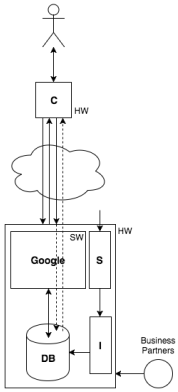
\includegraphics[scale=1]{figures/cs.png}
\caption{Architettura Client-Server} 
\end{figure}
\end{center}

La nuvola rappresenta Internet, un insieme dinamico di connessioni, mentre il Client è una macchina (HW) al cui interno risiede il SW. Tramite l’inserimento dell’url nel browser viene generato un round-trip. Una volta stabilita la connessione con il DBMS sarà possibile accedere alle informazioni che risiedono nel DB. Ad esempio la ricerca delle parole: “Cinema Lecce” restituirà tutte le occorrenze dell’intersezione degli insiemi costituiti dai risultati di ricerca delle due singole parole. Sui computer di proprietà di Google oltre al DBMS esistono altri software: \textbf{Spider} o \textbf{Crawler} e \textbf{Indexer}. 

Supponiamo che il web sia un grafo connesso, ovvero che ogni pagina web che risponde ad un url contenga i riferimenti (url) ad altre pagine web e così via, fornendo un url allo Spider esso ricorsivamente percorre tutto il grafo passando ciascuna pagina visitata all’Indexer. L’Indexer ha il compito di effettuare lo stamming delle parole ovvero la loro estrazione ed il mantenimento dei riferimenti alle pagine cui sono state trovate. L’idea pertanto consiste nel mantenere un indice analitico delle parole e i riferimenti a tutte le pagine web che le contengono. Questo consente di riuscire ad immagazzinare tantissimi riferimenti utilizzando pochi gigabytes. Quindi quando vogliamo effettuare una ricerca nel web ricorrendo ad un motore di ricerca le ricerche in realtà sono state già effettuate e l’unica cosa che fa il software è incrociare le informazioni. Google viene pagata da altre grosse società per far salire in cima i risultati delle ricerche per i contenuti che le riguardano. Osserviamo che l’ipotesi di rappresentazione del web attraverso un grafo connesso non è rappresentativa di alcune realtà come quella del deep web. Il deep web è costituito da isole cioè porzioni di grafo non connesse a quelle del web pertanto non raggiungibili sebbene nelle isole vengano utilizzati gli stessi protocolli del web (HTTP, ecc.).   

\subsection{Organizzazioni}

Per quanto concerne le persone che hanno a che fare con un sistema SW, possiamo distinguere tre tipologie principali: \{\textbf{User}, \textbf{Consumer}, \textbf{ Customer}\}. Per quanto riguarda le modalità di interazione e comunicazione con un sistema SW, troviamo la tipica architettura \textbf{\textit{Client-Server (C/S)}} e la \textbf{\textit{Peer-to-peer (P2P)}}. Nel P2P le entità in gioco sono tutte alla pari, nel senso che avvengono degli scambi alla pari di informazioni. Internet è oggigiorno dominata da questi due meccanismi. Abbiamo cominciato a vedere una prima tipologia, gli user, che sono però una parte di tutto il resto: gli \textbf{stakeholders} che letteralmente sono dei portatori di interesse, qualcuno interessato ad un sistema. Gli \textbf{UT} (\textit{User Types}) sono un sottoinsieme degli Stakeholders. Ad esempio, il rettore è uno stakeholder, ma non un utente. A volte sono proprio loro che comandano il tutto! Egli potrebbe pure non interagire con il SW, decide però le regole in gioco. Per parlare di uno stakeholder bisogna necessariamente precisare il sistema: per Google ad esempio, Ferrari è uno stakeholder particolare, denominato \textbf{business partner}. 
Parliamo ora di \textbf{Sistema} ed \textbf{Organizzazione}. Cos'è un'organizzazione? Esistono le persone e poi le organizzazioni. L'Università è un tipico esempio di organizzazione: struttura di persone che svolgono dei compiti ed hanno delle responsabilità, esse si occupano tipicamente di prodotti e di servizi. All'interno di un'azienda non vi può essere soltanto il singolo venditore, tipicamente vi è anche una fitta rete di assistenza. Noi abbiamo sempre a che fare con bundle di prodotti e servizi, ad esempio il comune telefono è un prodotto ed un servizio allo stesso tempo pertanto oggi quasi tutto è quindi un bundle di prodotti e servizi.  
Per schematizzare una tipica organizzazione possiamo avvalerci del modello di Anthony, che prevede una suddivisione piramidale dell'organizzazione in tre parti o livelli: Direzione, Management ed Operativa. Nell'Università ad esempio abbiamo il rettore, i presidi ed i professori e tecnici, stesso discorso per banche, ospedali, etc. La direzione è costituita da uno o pochi individui o da un consiglio di amministrazione, poi c'è il manager, il quale non è il capo dell'azienda: è il vice-capo ma risponde al direttore. I manager sono, nell’esempio dell’università, i direttori di dipartimento. Il personale operativo è chiamato anche \textbf{Front Office}. Svolgere i compiti operativi all'interno dell'università. Non bisogna però confondere Ruolo e Persona. L'organizzazione può essere rappresentata da un \textbf{organigramma}, la carta che rappresenta gli organi che compongono l'azienda e che rappresentano, tipicamente, una struttura gerarchica. Le organizzazioni, per essere ben guidate, a meno che non presentino strutture di tipo rete, devono essere strutturate in modo gerarchico, in alcuni casi vi potrebbe addirittura essere una replicazione del modello gerarchico. Nel caso delle holding ad esempio la struttura è di tipo gerarchico ed ogni organizzazione costituente è a sua volta una struttura gerarchica. Il \underline{sistema informativo} esiste da sempre e non è costituito da bit! Esso è costituito da informazioni. Il \underline{sistema informatico} è rappresentato da computer e dalle reti. 
 
Sebbene le informazioni esistano da sempre il sistema informatico è piuttosto recente, infatti nel tempo può cambiare il processo di elaborazione delle informazioni, il quale insieme alle informazioni stesse costituisce il sistema informativo. Attualmente il sistema informativo esiste su sistemi informatici ma prima dell’avvento dei computer “viveva” sulla carta.  
Come si crea un sistema informativo per un particolare ruolo? Ad esempio, per un direttore, preside o professore. Il ruolo è svincolato dal soggetto fisico! Lo stesso Anthony, con la sua piramide, ci fornisce un grande supporto per l'attività di Analisi dei Requisiti. Sempre riferendoci alla struttura piramidale, possiamo individuare altri tre livelli che meglio identificano e raggruppano i differenti tipi di dati che vengono trattati dai ruoli che appartengono ai tre differenti livelli gerarchici: La \textbf {BI} (\textit{Business Intelligence}), l'\textbf{ERP} (\textit{Enterprise Resource Planning}), ed il \textbf{CRM} (\textit{Customer Relationship Management}). Nel primo livello troviamo tipicamente sistemi DSS (\textit{Decision Support Systems}). Invece nello strato intermedio troviamo sistemi per la gestione e pianificazione delle risorse all'interno di un'azienda. SAP ad esempio, nato inizialmente in seno ad IBM, produce software ERP per le aziende.  
Le risorse di un sistema si suddividono in: \textbf{RI} (\textit{risorse immateriali}), \textbf{RM} (\textit{risorse materiali}) e \textbf{RU} o \textbf{HR} (\textit{risorse umane, human resources}). L'Università, gestisce solo le informazioni dello studente! Le RM sono tangibili. Le RU sono il professore, i tecnici, gli amministrativi. Questi software, o sistemi più in generale, sono molto importanti e complessi allo stesso tempo. L’acronimo CRM sta per Customer Relationship Management, a questo livello sono immagazzinati i dati degli acquisti dei clienti e si possono attuare delle tecniche MBA, ovvero di Market Basket Analysis. Nei vari sistemi superiori al CRM, per aggregare i dati in informazioni di livello superiore, si sfruttano delle potenti tecniche di clustering, Business Intelligence e Machine Learning. Con questi sistemi possiamo digerire quantità potenzialmente grandi di dati. Le informazioni possono essere di tipo analitico e di tipo sintetico. A livello CRM abbiamo ad esempio solo informazioni analitiche, più dettagliate. Tali informazioni vengono via via aggregate nei livelli superiori, mediante tecniche di cui sopra. Ci siamo serviti quindi del triangolo DMO di Anthony per capire come funzionano le organizzazioni, le persone ed i processi che elaborano le informazioni. 
 
Un \textbf{database} è una raccolta di informazioni, il cui ciclo di vita può essere sintetizzato nell’acronimo \textbf{CRUD} (\textit{Create, Read, Update, Delete}). Le informazioni sono straordinariamente importanti. Sapere delle informazioni ci consente di procedere operativamente in determinate direzioni piuttosto che in altre. Imparare a progettare i sistemi informativi serve a risolvere concretamente vari problemi delle persone. Abbiamo quindi a che fare con un mondo di informazioni ed organizzazioni, le quali giacciono in complesse reti. Servono tecniche di modellazione e di soluzione del problema complessivo.  
Un'impresa consiste in delle risorse: RI, RM, RH. Qual è il valore associato a questi oggetti? Le risorse umane, dal punto di vista dell'organizzazione, hanno un enorme valore; costituiscono il valore stesso dell'azienda, sono delle risorse non alienabili la cui sostituzione può avere effetti negativi sull’azienda stessa. Anche le RM sono delle risorse importanti, possono essere vendute per creare valore. Tuttavia, rivestono una grande importanza le risorse immateriali, ovvero le informazioni. Basti pensare a cosa accadrebbe se venissero cancellati tutti i dati dal database dell'università!!! Le informazioni all'interno delle organizzazioni hanno un valore direttamente rapportabile a quello che l'organizzazione fa. Oggi il mercato è strutturato in: Primario, Secondario, Terziario e Terziario Avanzato. Noi ingegneri informatici ci collochiamo nel settore terziario. Facendo dei conti, considerando ad esempio il mercato telefonico, esso vale circa, a livello mondiale, un migliaio di miliardi di dollari. Questi soldi fanno girare un mercato enorme, ed in gioco vi sono degli interessi pazzeschi! Grandi aziende come Apple, Samsung, o Microsoft decidono del guadagno e della perdita di queste enorme moli di denaro. Oggi quando parliamo di Google o di Facebook, parliamo di tutto il mondo che c'è dietro. Trattano il settore della Comunicazione, ma lo mutano profondamente: "\textit{Bisogna creare il bisogno}", dicono gli esperti di marketing e dinanzi a una apparente frase banale, si celano queste importanti dinamiche, che un progettista informatico deve assolutamente sapere. Non si tratta più di questioni legate all'ottimizzazione del codice ad esempio! Le informazioni sono quindi le risorse fondamentali delle organizzazioni: è una dimensione molto importante da conoscere.  
 
Vediamo ora l'organizzazione come un Sistema Dinamico, che viene attraversato da input e produce in uscita degli output. Il direttore ha bisogno di conoscere i cosiddetti \textbf{KPI} dell'organizzazione (\textit{Key Performance Indicator}), per sapere se l'azienda sta andando bene o meno. Queste informazioni vengono interpretate attraverso il cosiddetto \textbf{cruscotto aziendale}. Alla stregua di una macchina, le aziende si guidano e chi le guida ha necessariamente bisogno di questo cruscotto. Le informazioni devono quindi essere sempre presenti. Un’organizzazione può essere vista come una black box, che riceve in ingresso Materie Prime ed informazioni, queste vengono elaborate mediante rispettivamente sistemi operativi ed informatici, e produce alla fine in output dei prodotti o servizi, ed altre informazioni. Troviamo i cosiddetti \textbf{EIS} (\textit{Enterprise Information System}) a tal proposito. 


\subsection{Lo scenario della progettazione - Progetto e realizzazione}

Come si colloca il concetto di modello nell’ambito dell’ingegneria? Consideriamo l’esempio dello scaldabagno: quando accendiamo il termostato la temperatura aumenta nel tempo con un andamento esponenziale fino a quando ad un certo punto non inizia a decrescere e così via. Una rappresentazione analitica di questo problema ci porterebbe intuitivamente a considerare la temperatura come una variabile rilevante mentre il colore della spia del termostato come una variabile irrilevante. Un \underline{\textbf{modello di analisi}}, quindi, è una rappresentazione minimale di un sistema fisico depurato dagli effetti secondari in cui possiamo identificare una relazione I/O utile ai nostri scopi. I \underline{\textbf{modelli di sintesi}} sono la concettualizzazione di un oggetto che sto creando.  Il \textbf{requisito} è il modo in cui si traduce la fattibilità tecnica del sistema che si sta progettando, i requisiti costituiscono le possibili soluzioni del problema. I Goal sono i motivi per cui mi rivolgo al progettista, essi vengono risolti dai requisiti. Il progettista ha l’obbligo di rendere al cliente dopo qualche giorno dall’intervista un modello concettuale (MC), un’astrazione del \textbf{modello fisico} del problema. Il \textbf{modello concettuale} deve rendere l’idea di come il progettista ha pensato di risolvere il problema, il tutto ricorrendo ad un linguaggio comprensibile per il committente e facendo uso di illustrazioni grafiche, i Mockups. Il progettista ha a disposizione pochissimi minuti per illustrare la sua idea al committente e a convincerlo della buona riuscita del suo lavoro. 
 
Dal momento che il committente in generale può essere incerto sulle richieste e potrebbe cambiarle in corso d’opera si redige un documento formale in cui si fissano i requisiti e si fanno firmare dal committente. Questa fase non è remunerativa pertanto è consigliabile non sprecare risorse economiche. Qualora il modello concettuale dovesse andar bene si firma un contratto tra le parti ed il committente è tenuto a dare un acconto. Il \textbf{modello logico} (ML) è un documento tecnico interpretabile da professionisti e tecnici esperti del dominio in cui sono contenute informazioni dettagliate circa lo sviluppo del progetto. Occorre definire uno standard di interfaccia tra il team e il progettista. Il team prende visione anche del modello concettuale ed infine produce il \textbf{modello fisico} (MF). Nella fase di progettazione iniziale è fondamentale predisporre anche tutti i casi di test nonché le possibili eccezioni per poi verificarle man mano che blocchi del software vengono costruiti. Il consulente è un professionista, generalmente un analista, che viene pagato dal committente per supervisionare esternamente tutto il processo di sviluppo del software e per curare i suoi interessi. Il suo compito consiste nel controllo del progettista, del team, supervisiona le release intermedie del SW e si occupa anche di collaudarlo. 

\begin{center}
\begin{figure}[H]
\centering
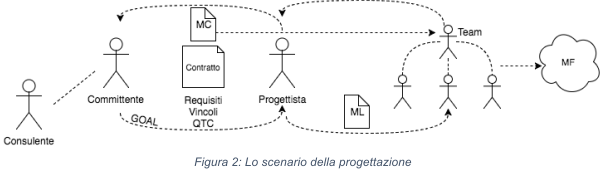
\includegraphics[scale=0.8]{figures/mdlng.png}
\caption{Scenario della Progettazione} 
\end{figure}
\end{center}

\begin{flushright}Marco Chiarelli\\Gabriele Accarino\\28/09/2016\end{flushright}

\subsection{Scenario Ingegneristico della Progettazione}

Goal + requisiti + vincoli + test = contratto

\begin{center}
\begin{figure}[H]
\centering
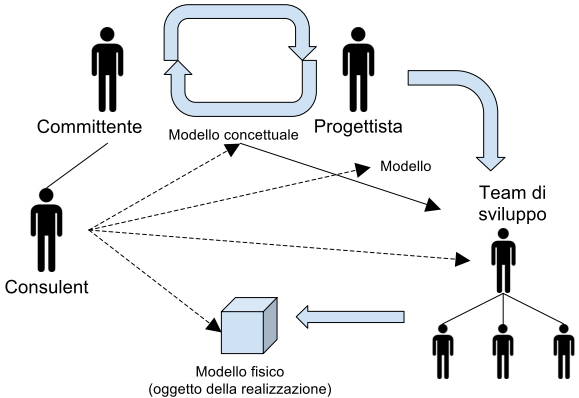
\includegraphics[scale=1]{figures/mdlng2.png}
\caption{Scenario della Progettazione} 
\end{figure}
\end{center}

Lo scenario tipico del progetto ingegneristico è il seguente: abbiamo un \textbf{committente} che richiede un \textbf{prodotto} (nel caso dell’ingegneria informatica, un’applicazione), un \textbf{progettista} che, parlando col cliente, estrae i goal del progetto, i requisiti, i vincoli di qualità, tempo e costo e i test da effettuare e dà al committente un documento, chiamato \textbf{modello concettuale} che conterrà le stime dei costi e del risultato finale del prodotto (nel caso di progetti legati al mondo dell’informatica, spesso corrispondono ai mockup) che si assocerà, alla fine, al \textbf{contratto}. Il progettista raffina il suo modello concettuale creando un altro documento che si chiama \textbf{modello logico} (che contiene i calcoli e specifiche tecniche maggiori di quelle presenti nel modello concettuale) e, insieme al modello concettuale, sarà la base da cui partiranno i \textbf{membri del team di sviluppo} (composta generalmente da un team leader e dagli sviluppatori) e si occupa di trasformare i modelli logico e concettuale, nell’\textbf{oggetto della realizzazione} (nell’ingegneria informatica corrisponde col \textbf{modello fisico}). Il committente, per assicurarsi che il lavoro sia corretto e con un buon rapporto qualità prezzo, si affida ad una terza figura, il \textbf{consulente} che, grazie alla sua esperienza pregressa, affianca il committente per verificare ogni fase del progetto.   
Le risorse materiali costano poco nella fase di sviluppo di un progetto dell’ingegneria informatica, il costo maggiore in un progetto lo si ha nelle risorse umane e immateriali. Avendo questa importante informazione, questo modello ci permette di fare una stima dei costi molto precisa: si utilizzano i \textbf{\textit{function points}} che, data una serie di specifiche, permettono di capire quanto tempo ci vuole per realizzarle. Dato il tempo di sviluppo in anni uomo, si può semplicemente moltiplicare questo valore per il costo annuo di uno sviluppatore per avere il costo totale del progetto. A questa documentazione bisogna aggiungere anche la \textbf{matrice RACI} che serve per dire “chi ha fatto una determinata parte del progetto” in modo da dare all’azienda produttrice la possibilità di tracciare la qualità di un ingegnere o di uno sviluppatore. Ricapitolando, un modello può essere fatto per il committente o per i membri del team ma, indipendentemente, è un insieme di regole e simboli noti (per esempio, in un modello dell’architettura di una casa, un segmento con un arco di circonferenza di 90 gradi indica una porta). Nel mondo dell’ingegneria informatica, i modelli statici e dinamici sono tipicamente logici, ma possono anche essere usati nel modello concettuale da mostrare al committente. Per esempio, se volessimo creare un gioco di scacchi, dovremmo creare nel diagramma delle classi una classe “casella”, una classe “scacchiera” (aggregazione di caselle), dopodiché si crea una classe generica “pezzo” che verrà implementata diversamente per ogni pezzo (pedoni, cavalli, alfieri, ecc…). Questo tipo di progettazione, dove il modello guida la progettazione, si chiama \textit{\textbf{model driven engineering}}. Si usano le tecniche di modellazione come quelle di \textit{\textbf{forward e reverse engineering}}. La prima permette, guardando il modello, di creare il software; viceversa la seconda. Ogni tipo di progettazione ha un limite. Nel caso della progettazione \textit{model driven} si ha che il \textit{reverse engineering} ha un costo e non è del tutto automatico, quindi ciò porta ad avere casi in cui si inizia creando il modello, si crea il codice e si modifica la struttura senza modificare il modello. Se si cambiano parti di un progetto senza modificare il modello a lungo andare si dimenticherà il motivo di tale modifica. Per questo motivo sono nati i processi di \textbf{BPR} (\textit{business process re-engineering}). Tale processo, chiamato anche “prato verde”, permette ai nuovi team di evolversi autonomamente, senza l’obbligo di seguire metodi precedentemente utilizzati.


\section{Architettura di un Progetto Software}

\subsection{L'hardware}

Ogni calcolatore è basato sul modello della macchina di Von Neumann che presenta una parte logica (CPU), una o più memorie, uno o più dispositivi di input/output e un bus che collega il tutto. 

\begin{center}
\begin{figure}[H]
\centering
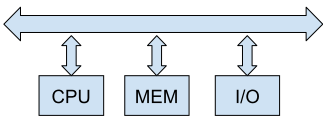
\includegraphics[scale=1]{figures/vonmn.png}
\caption{Modello della macchina di von Neumann} 
\end{figure}
\end{center}

La CPU contiene le unità ALU (\textit{Arithmetic and Logic Unit}), FPU (\textit{Floating-Point Unit}), CU (\textit{Control Unit}) e dei registri. La memoria contiene i programmi (la sequenza di istruzioni) e i dati. In questo modello, il calcolatore, al suo avvio, esegue l’istruzione alla posizione numero 0, poi la sua successiva e così via in \textbf{sequenza}. Il modello di Von Neumann permette anche di variare il flusso di esecuzione, attraverso la comparazione e il salto. Possiamo dividere un’architettura software in diversi livelli. Il primo livello che si può trovare è il \textbf{livello hardware}, che si basa sul modello della macchina di Von Neumann. Il livello successivo è il \textbf{livello macchina} che implementa le istruzioni di esecuzione (DO), di comparazione (CMP) e di salto (JMP) nel linguaggio macchina. Questo tipo di programmazione è di tipo \textbf{imperativo sequenziale}. La sequenza può essere variata tramite CMP e JMP. Il linguaggio macchina è composto da un alfabeto di 2 caratteri (0 e 1) quindi troppo di basso livello per l’essere umano. I linguaggi che implementano queste istruzioni si chiamano \textbf{linguaggi assemblativi} (Assembly è il più famoso), nel corrispettivo livello (\textbf{livello assemblativo}). Un comando a livello assemblativo corrisponde a una serie di istruzioni a livello macchina. Il risultato di questo tipo di programmazione è anche chiamato \textbf{codice spaghetti}, dato dal grande numero di salti tra le varie righe di codice. Il \textbf{linguaggio strutturato} viene introdotto per ridurre gli errori causati dal livello assemblativo, ancora di livello troppo basso e per l’eccessiva libertà che si ha nel programmare. I linguaggi che fanno parte di questa categoria sono il C, il FORTRAN, il Pascal, e il Basic. La caratteristica di questi linguaggi è quella di avere le strutture di controllo (if, while, for, ecc…), che sono una unione di più comandi di livello assemblativo. 
   
Il livello successivo è il \textbf{livello a oggetti}, o OODP (object oriented design and programming) che contiene i linguaggi Java, C++, Eiffel, Ruby, Python e molti altri. Questo tipo di linguaggi ha 3 particolari caratteristiche: ereditarietà, polimorfismo e incapsulamento. L’\textbf{ereditarietà} è quella caratteristica che permette il riuso e l’estensione delle classi e del codice (utilizzando le librerie di classe). Il \textbf{polimorfismo} si applica ai metodi delle classi. Permette di avere uno stesso metodo che agisce in modo diverso a seconda del tipo di classe che gli viene passato (per esempio, la somma di 1 e 2 è diversa se queste variabili sono interi o stringhe). Il principio dell’\textbf{incapsulamento} impedisce di modificare degli attributi o richiamare metodi “privati” dall’esterno della classe stessa. Questo principio permette di non avere dei \textit{side effect} che si avrebbero invece nei linguaggi strutturati. Il problema di questo livello è che non c’è un mapping diretto tra i modelli e gli oggetti (ci sono algoritmi chiamati ORM che cercano di risolvere questo problema, ma non sempre ci riescono perfettamente). 

\begin{center}
\begin{figure}[H]
\centering
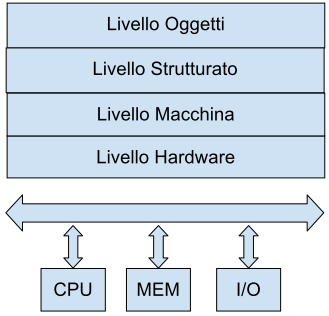
\includegraphics[scale=1]{figures/hwsw.png}
\caption{Architettura hardware-software} 
\end{figure}
\end{center}

\subsection{Il software - Architettura a tre livelli}

Un software che utilizza una base di dati (data-centric application) può essere decomposto in tre parti: il \textbf{data layer} è il livello dove vengono salvati i dati (il database), il \textbf{business rule layer} è il livello logico del progetto, il \textbf{presentation layer} è il livello che permette di far interagire l’utente con l’applicazione (può essere un messaggio su schermo, un comando vocale, un’interfaccia a gesture, ecc…).  
Nella storia, il presentation layer si è evoluto con l’avanzare della tecnologia:

\begin{itemize}

\item quando si programmava utilizzando il linguaggio macchina, gli input erano le schede perforate e i nastri magnetici;
\item con il linguaggio assemblativo sono stati introdotti i primi comandi a riga di comando (con l’introduzione dei monitor);
\item con l’evoluzione a livello strutturato si è arrivati al concetto di WIMP (windows, icons, menus, pointers) che ha rivoluzionato l’utilizzo dei calcolatori;
\item infine si ha l’evoluzione della WIMP in GUI (Graphic User Interface), l’introduzione delle gesture, delle interfacce vocali e delle percezioni aptiche. 

\end{itemize}

\begin{center}
\begin{figure}[H]
\centering
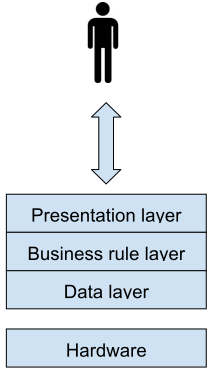
\includegraphics[scale=1]{figures/tla.png}
\caption{Architettura software a tre livelli} 
\end{figure}
\end{center}

\begin{flushright}Emanuele Costa Cesari\\Paolo Panarese\\29/09/2016\end{flushright}

\section{Modellazione dei dati}

Argomento centrale della lezione: \textbf{MODELLAZIONE DEI DATI}. Ripartiamo brevemente da ciò che nelle scorse lezioni abbiamo chiamato scenario ingegneristico della progettazione. Impareremo a costruire tre tipi di modelli: modello concettuale, modello logico e modello fisico. Ricordiamo qual è il ruolo di ognuno di essi.  

\begin{center}
\begin{figure}[H]
\centering
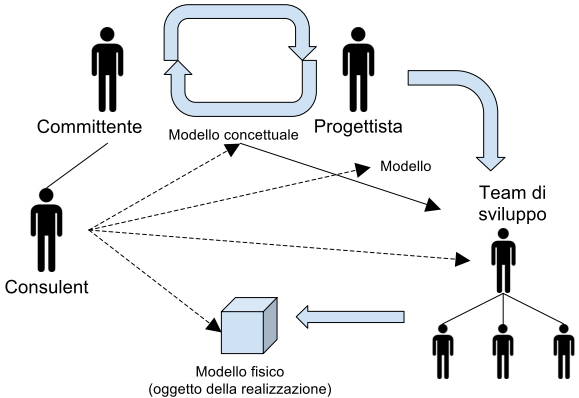
\includegraphics[scale=1]{figures/mdlng2.png}
\caption{Scenario della Progettazione} 
\end{figure}
\end{center}

Lo scenario tipico del progetto ingegneristico è il seguente: un \textbf{committente} che richiede un \textbf{prodotto} (nel caso dell’ingegneria informatica, un’applicazione), si rivolge ad un \textbf{progettista} che estrae i goal del progetto, i requisiti, i vincoli di qualità, tempo e costo e i test da effettuare. Il progettista produce per il committente un documento, chiamato \textbf{modello concettuale} che conterrà la stima dei costi e del risultato finale del prodotto (nel caso di progetti legati al mondo dell’informatica, spesso corrisponde al mockup). Il progettista raffina il modello concettuale creando un altro documento, il \textbf{modello logico} (che ha finalità più tecniche, contiene calcoli e specifiche tecniche). Modello concettuale e modello logico saranno la base da cui partiranno i membri del \textbf{team di sviluppo} (organizzato tipicamente in forma gerarchica, composta da un team leader e dagli sviluppatori) per trasformare queste informazioni nell’\textbf{oggetto della realizzazione} (nell’ingegneria informatica corrisponde con il modello fisico). Il committente, per assicurarsi che il lavoro sia corretto e con un buon rapporto qualità-prezzo, si affida ad una terza figura, il \textbf{consulente} che ha la responsabilità di supervisionare e verificare ogni fase del progetto.  È importante tenere presente che il progettista deve essere abile a presentare e mettere a confronto diverse soluzioni per il medesimo problema. Ogni soluzione deve specializzare un aspetto in particolare, perché committenti diversi potrebbero essere interessati a diversi aspetti dello stesso problema e magari vorranno porre enfasi su uno di questi. Un buon progettista deve saper dare una direzione alle idee, impostare una strategia di risoluzione. In qualità di ingegneri, dobbiamo essere in grado di creare modelli, di progettare una soluzione sia dal punto di vista visuale, che tecnico, che quantitativo. Per disegnare e particolareggiare ogni aspetto della modellazione ci si avvale di un insieme di strumenti. Un esempio nel caso di modellazione di software è UML, che è una raccolta di diversi tipi di diagrammi, ognuno dei quali aiuta il progettista a descrivere un particolare aspetto di ciò che deve realizzare. Per progettare sono quindi necessarie diverse abilità, perché bisogna modellare diversi aspetti. Nell’ambito dell’ICT distinguiamo tre aspetti principali:

\begin{itemize}

\item Hardware (ex. processor, display, elementi di networking, ecc.);
\item Software (ex. sistema operativo, software applicativo, driver, ecc.);
\item Dati: Un progetto non è ben progettato se non vengono considerati tutti e tre gli aspetti sopra elencati.

\end{itemize}

Un progetto non è ben progettato se non vengono considerati tutti e tre gli aspetti sopra elencati. 

\subsection{ESEMPIO – APPLICAZIONE CLIENT-SERVER}

Nella figura sottostante è rappresentata la struttura hardware di un’applicazione Client-Server: c’è un client connesso a Internet attraverso un ISP e un dispositivo chiamato Google Server. Queste due macchine sono collegate dal punto di vista hardware da una rete, basata su tecnologie come TCP/IP. Quello hardware non è l’unico livello da considerare, bisogna occuparsi anche della parte software. Infatti un dispositivo avrà bisogno di un sistema operativo e di applicazioni. 

\newpage
\begin{center}
\begin{figure}[H]
\centering
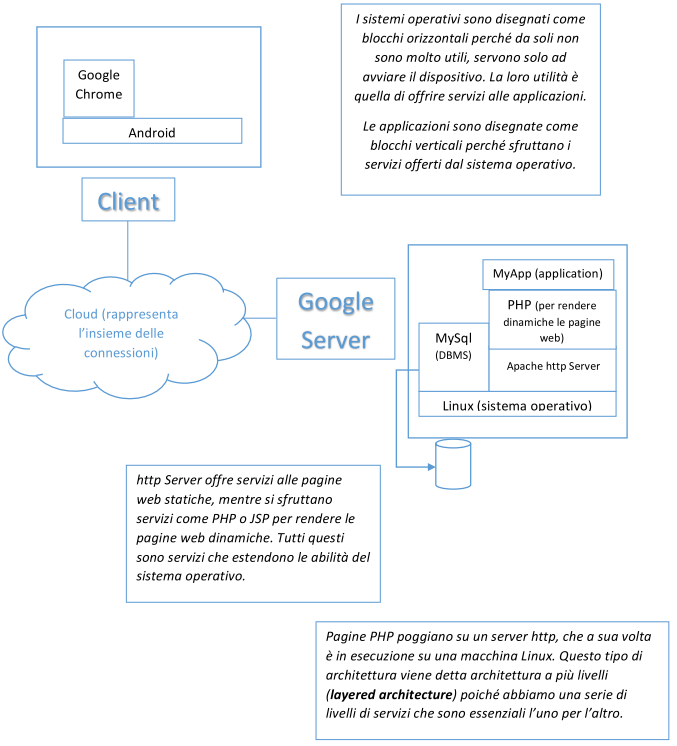
\includegraphics[scale=0.8]{figures/google_cs.png}
\caption{Scenario Google Client-Server} 
\end{figure}
\end{center}
\newpage

Il Server Hardware è una macchina destinata a soddisfare richieste. Quando si disegna l’architettura software si progetta il tipo di software da inserire nella macchina hardware e le richieste che potranno essere realizzate. Infine, bisogna progettare anche un’architettura dati.  
Oggi disegneremo la nostra prima Data Architecture. Come fare?  In generale quando parliamo di Software Engineering, le architetture sono disegnate in termini di classi. Ogni classe è specificata da un nome, degli attributi e dei metodi. Le classi possono interagire tra loro ed esistono diversi tipi di relazioni tra di esse: una classe può utilizzare un’altra classe, aggregarla, specializzarla, ecc.  Il problema sorge quando bisogna mappare queste classi in Data Structures per gestire la persistenza e la serializzazione dei dati.  Si dice che un’applicazione è in grado di gestire la persistenza dei dati se questi sopravvivono a diverse sessioni di utilizzo dell’applicazione.  Dare alle classi la possibilità di realizzare la persistenza dei dati non è sufficiente, poiché si ha anche la necessità di lavorare con essi. Normalmente facciamo utilizzo di database non solo per memorizzare dati, ma anche per recuperarli in un ordine differente da quello utilizzato per memorizzarli.  Abbiamo bisogno di eseguire diverse operazioni sui dati: crearli, cancellarli, modificarli, trasformarli, ecc. Per fare questo utilizziamo delle funzioni di alto livello, come le Associative Functions.  Riscrivere queste funzioni ogni volta che scriviamo un programma è molto dispendioso e poco pratico. Perciò si utilizza un \textbf{DBMS} (\textbf{DataBase Management System}) come MySql, un software orientato al data processing, che rappresenta i dati in maniera differente. Un DBMS organizza in “librerie” le funzioni di cui abbiamo bisogno per l’elaborazione dei dati. Utilizzare le funzioni di alto livello fornite da un DBMS rende il nostro codice più efficiente e la programmazione più veloce e meno costosa. Quindi non è necessario che le nostre classi gestiscano direttamente la persistenza e implementino funzioni di ricerca, perché abbiamo a disposizione del software specifico che si occupa della gestione dei dati. Non scriveremo codice in termini di Object Oriented code, ma faremo quello che è chiamato \textbf{ORM} (\textbf{Object Relational Mapping}). Un esempio di Object Relational Mapper è Hibernate. Per esempio, possiamo scrivere un programma Java che richiede dati ad un database relazionale. Un ORM come Hibernate si occupa di trasformare le richieste delle classi Java in richieste al database, traducendo le operazioni sugli Oggetti in operazioni su Tabelle del database. La progettazione di un’applicazione richiede la realizzazione di questi passi:

\begin{itemize}

\item Goal;
\item Requisiti;
\item Architettura Sw, Architettura Hw, Architettura dati;
\item Test e deployment;
\item Operation

\end{itemize}


\subsection{ESEMPIO}

Iniziamo	a	vedere	come	modellare	concettualmente	i	dati.	Data	una	situazione	come	quella	descritta	dall’Entity	Relationship	Diagram	in	figura,	un	ingegnere	deve	essere	in	grado	di	immaginare	come	sarà	il	software.	

\begin{comment}
\centering
%\scalebox{.87}{
\begin{tikzpicture}[node distance=5cm, every edge/.style={link}]

\node[entity] (cus) {Customer};
\node[attribute] (name) [below of=cus] {Name} edge (cus);
\node[attribute] (addr) [below right of=cus] {Address} edge (cus);
\node[attribute] (bdat) [below left of=cus] {B\_Date} edge (cus);
\node[attribute] (fdat) [left of=bdat] {F\_Date} edge (cus);

\node[relationship] (buys) [right of=cus] {Buys} edge(cus);
\node[attribute] (dat) [below of=buys] {Date} edge(buys);
\node[attribute] (qnt) [below right of=buys] {Quantity} edge(buys);
\node[attribute] (spr) [below left of=buys] {Selling price} edge(buys);

\node[entity] (prod) [right of=buys] {Product} edge(buys);
\node[attribute] (pc) [below of=prod] {PC} edge(prod);
\node[attribute] (pnam) [below right of=pc] {Name} edge(prod);
\node[attribute] (ppic) [below left of=prod] {Picture} edge(prod);
\node[attribute] (desc) [right of=pnam] {Description} edge(prod);
\node[attribute] (lprc) [left of=ppic] {List price} edge(prod);

\end{tikzpicture}
%}
\end{comment}

\begin{center}
\begin{figure}[H]
\centering
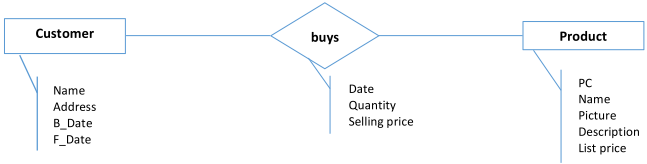
\includegraphics[scale=0.8]{figures/ERD.png}
\caption{Entity Relationship Diagram} 
\end{figure}
\end{center}

\textbf{Customer} e	\textbf{Product} prendono	il	nome	di	entità,	poiché	possono	esistere	anche	da	sole,	sono	definite	senza	dipendere	dagli	altri	elementi	del	database. \textbf{Buys} è	una	\underline{\textit{\textbf{relazione}}}	e	non	può	esistere	da	sola,	dal	momento	che	non	avrebbe	alcun	significato	se	posta	fuori	da	un	contesto	(esempio:	non	posso	definire	un	acquisto	senza	indicare	l’acquirente	e	il	prodotto	acquistato).	Possiamo	rappresentare	un	database	come	un	grafo,	in	cui	ogni	\textbf{Entità}	è	un	nodo	e	ogni	\textbf{Relazione}	è	un	arco.	Su	questo	grafo	possiamo	individuare	diversi	percorsi,	che	corrispondono	a	interrogazioni	al	database	(query).

\subsection{ESEMPIO - THE COMPANY DATABASE}

Facciamo	un	passo	in	avanti	analizzando	qualcosa	di	più	complesso.	Consideriamo	l’esempio	\textit{The	Company	Database} del	libro	di	testo.	

\begin{center}
\begin{figure}[H]
\centering
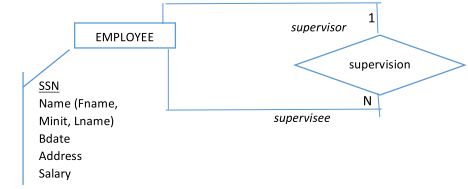
\includegraphics[scale=1]{figures/tcd.png}
\caption{The Company Database} 
\end{figure}
\end{center}

Notiamo	che:

\begin{itemize}

\item L’attributo	SSN	dell’entità	employee	è	sottolineato.	Con	la	sottolineatura	si	indica	la	\textbf{chiave	primaria},	ovvero	l’attributo	(o	l’insieme	di	attributi)	che	identifica	univocamente	un’istanza	di	una	certa	entità.	Non	potranno	esistere	due	employees	aventi	attributo	SSN	con	lo	stesso	valore;
\item I	numeri	indicano	la	\textbf{cardinalità}	della	relazione.	Nell’esempio	abbiamo	che	un	employee	può	supervisionare	N	employees	ed	un	employee	può	essere	supervisionato	da	un	solo	employee	(relazione	uno-a-molti).

\end{itemize}

Espandiamo	lo	schema	precedente,	aggiungendo	altre entità...

\newpage
\begin{center}
\begin{figure}[H]
\centering
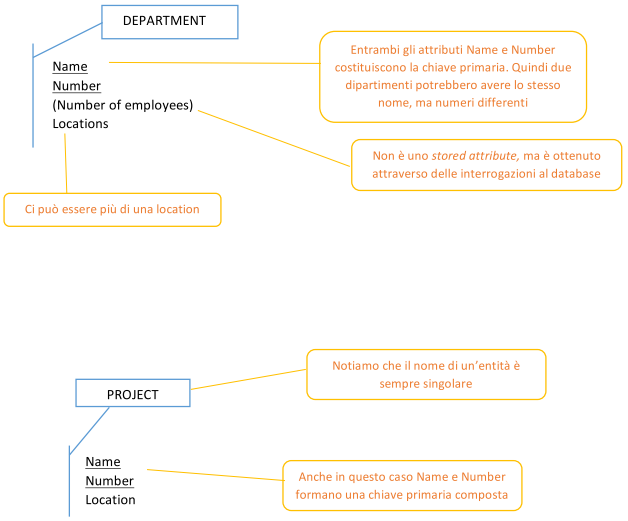
\includegraphics[scale=0.8]{figures/tcdBIG.png}
\caption{The Company Database} 
\end{figure}
\end{center}
\newpage

... e	le	relazioni	che	intercorrono	tra	di	esse:

\begin{center}
\begin{figure}[H]
\centering
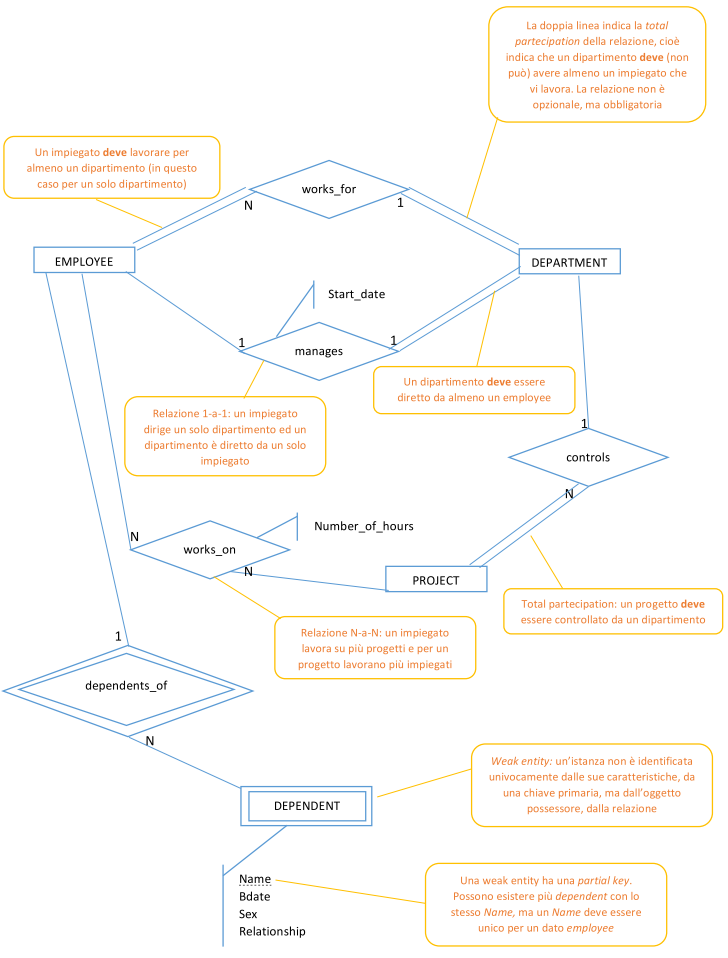
\includegraphics[scale=0.8]{figures/tcdBIG2.png}
\caption{The Company Database 2} 
\end{figure}
\end{center}

\begin{flushright}Floriana Accoto\\Emanuele Trono\\05/10/2016\end{flushright}


\section{Conceptual Model}

Nella lezione precedente abbiamo visto come realizzare il data modeling, composto da CM (Conceptual model), LM (Logical model), FM (Physical model). 
Gli elementi principali del CM sono tre: Entity type, Relation type, Attributes.

\begin{center}
\begin{figure}[H]
\centering
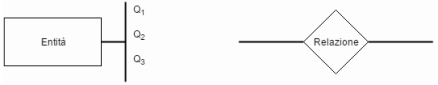
\includegraphics[scale=1]{figures/ER.png}
\caption{Elementi CM} 
\end{figure}
\end{center}

Combinando questi elementi si crea il CM. Naturalmente esistono delle regole e dei vincoli da rispettare, in quanto si sta parlando di un linguaggio formale. Ad esempio non sono consentite operazioni del genere:

\begin{center}
\begin{figure}[H]
\centering
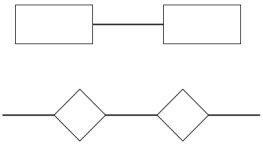
\includegraphics[scale=1]{figures/ERcomb.png}
\caption{Operazioni proibite in un ER} 
\end{figure}
\end{center}

vale a dire non è possibile collegare direttamente due entità o due relazioni. 

La logica da seguire è la seguente,

\begin{center}
\begin{figure}[H]
\centering
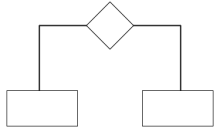
\includegraphics[scale=1]{figures/correctER.png}
\caption{ER corretto} 
\end{figure}
\end{center}

tenendo conto che le entità devono avere necessariamente degli attributi, mentre le relazioni possono anche non averne. 

Il modello concettuale fornisce anche i seguenti vincoli:

\begin{itemize}

\item Cardinalità;
\item Total Participation;
\item Primary Key.

\end{itemize}

Per ogni entità partecipante ad una relazione viene specificata una cardinalità di relazione. Essa è una coppia di numeri naturali che specifica il numero minimo e massimo di istanze di relazione a cui un’istanza dell'entità può partecipare. Esistono tre tipi di cardinalità: 

\begin{itemize}

\item 1 a 1;
\item 1 a molti;
\item Molti a molti.

\end{itemize}

Nell’ultimo caso conviene mettere due lettere differenti perché riportare la stessa lettera (ad esempio n to n) fa capire che le entità possiedono lo stesso numero di partecipanti, ma questo è errato. Infatti non si è in 
grado di prevedere a priori il numero esatto dei partecipanti, portando il progettista a fornire un’informazione errata del modello. 

Vediamo degli esempi, per comprendere meglio come differenziare i vari tipi di cardinalità: 

\begin{itemize}

\item

\begin{center}
\begin{figure}[H]
\centering
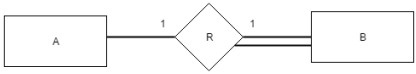
\includegraphics[scale=1]{figures/ER11.png}
\caption{Relazione 1 a 1 $\rightarrow$ A (person) - R(has) – B (Driving license)} 
\end{figure}
\end{center}

La patente è un’entità che esiste anche se non ha un possessore, così come la persona, ed ha come attributi numero, ente, data di rilascio, ecc. In questo caso ha senso parlare di totally partecipation solo nel caso della patente, che non può non essere associata ad una persona. Mentre la persona non deve necessariamente avere una patente e potrebbe avere come attributi il nome, cognome, codice fiscale. 
N.B. Un esempio errato è quello di definire come entità il codice fiscale di una persona. Infatti ogni individuo possiede un codice fiscale che lo caratterizza, ma il codice fiscale è un’attributo dell’entità persona, in quanto è una caratteristica della persona. Inoltre possiamo affermare che il codice fiscale è un autonomous entity type.

\item{}

\begin{center}
\begin{figure}[H]
\centering
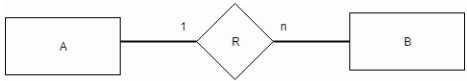
\includegraphics[scale=1]{figures/ER1n.png}
\caption{Relazione 1 a molti $\rightarrow$ A (Person) – R (Own) – B (Car)} 
\end{figure}
\end{center}

È una relazione uno a molti poiché una persona può possedere più macchine, al contrario una macchina non può essere posseduta da più persone. Di conseguenza, in questo caso, non si può parlare di total participation, perché una persona può non avere un’auto e un’auto può non avere un proprietario.

\item{}

\begin{center}
\begin{figure}[H]
\centering
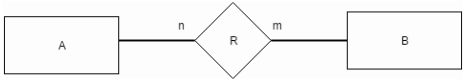
\includegraphics[scale=1]{figures/ERnm.png}
\caption{Relazione molti a molti $\rightarrow$ A (Car) – R (Has) – B (Optional)} 
\end{figure}
\end{center}

Questo tipo di relazione ci permette di introdurre il concetto di pattern, di cui si parla nell’appendice. 

\end{itemize}

\subsection{Il valore NULL}

Il valore NULL è un valore speciale in un DB, infatti la PK (chiave primaria), cioè un singolo raggruppamento di attributi dell’entità che ci permette di identificare univocamente un’istanza dell’entità stessa, deve essere necessariamente di tipo NOT NULL, vediamo il perché.  
È buona norma evitare di inserire valori di tipo NULL all’interno del DB, in quanto sono indice di mancanza di informazioni e al momento dell’estrazione dei dati, non si potrà comprendere se il dato non è stato inserito, se non se ne conosce il valore, se c’è stato un errore in fase di inserimento ecc. 
Pertanto la presenza di valori di tipo NULL significa che non solo non si conosce il valore di un determinato attributo, ma non si sa neanche il motivo per cui quel valore non è presente.  
La maniera corretta di inserire in un DB devi valori nulli è quella di inserire delle stringhe vuote. Ad esempio se si vuole inserire in un record una persona che non ha un secondo nome, mentre tra gli attributi dell’entità persona compare, il modo corretto di procedere è quello di inserire una stringa vuota, cioè “”. 
ESEMPIO: Se si volesse calcolare l’età media di un gruppo di persone inserite in un DB, è sufficiente che ci sia un unico campo in cui compaia un valore di tipo NULL per fare non essere in grado di calcolarla. In quel caso si potrà avere solo una stima dell’età media, ma non l’età media esatta.

\[
	3 + 2 + NULL = NULL
\]

\subsection{ANALIST}

\begin{center}
\begin{figure}[H]
\centering
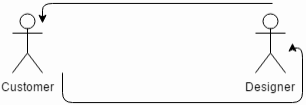
\includegraphics[scale=1]{figures/custdes.png}
\caption{Customer \& Designer} 
\end{figure}
\end{center}

\subsection{SCHEMA}

\begin{center}
\begin{figure}[H]
\centering
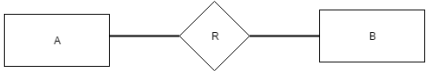
\includegraphics[scale=1]{figures/ERschema.png}
\caption{Schema ER} 
\end{figure}
\end{center}

È importante capire che gli schemi di database usati nei precedenti esempi forniscono una INTENTIONAL DESCRIPTION OF DATABASE, cioè, mediante l’uso di un linguaggio formale si è in grado di fornire una descrizione logica del database. Si useranno ora nuovi elementi che portano a fornire una EXTENSIONAL DESCRIPTION OF DATABASE. Rientrano in questa categoria: 

\begin{itemize}

\item Tabelle;
\item Entity Set.

\end{itemize}

Le tabelle in un database relazionale sono un insieme di elementi che sfruttano un modello in cui ci sono colonne verticali (ogni colonna è identificata con il nome di un attributo) e righe orizzontali, dove la cella del database rappresenta il punto in cui colonna e riga si intersecano. Ogni tabella del database coincide con l’entità presa in analisi, dove le colonne rappresentano gli attributi. Se la quantità degli attributi ha un valore fissato, le righe invece hanno un valore variabile in quanto rappresentano il numero di istanze contenute 
nell’entità. La riga di una tabella prende il nome di record della tabella. Le tabelle sono alla base delle relazioni. 
Un altro tipo di EXTENSIONAL DESCRIPTION OF DATABASE non si basa sull’uso delle tabelle ma sulla SET THEORY. Per poter fornire la definizione di entity set, bisogna definire che cos’è un entity type. Un entity type definisce una collezione (o set) di entità che hanno gli stessi attributi. Ogni entity type è descritto dal nome e dai suoi attributi. La collezione di tutte le entità di un particolare entity type nel database in qualsiasi punto nel tempo è chiamato entity set o entity collection.

\begin{center}
\begin{figure}[H]
\centering
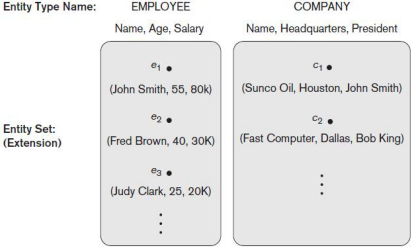
\includegraphics[scale=1]{figures/entity_set.png}
\caption{Entity Set} 
\end{figure}
\end{center}

L’obiettivo che ci si pone è quello di usare uno stesso DB per soddisfare più bisogni.  
ES. Una catena di negozi, che ha sedi diverse, utilizza copie dello stesso DB per registrare gli acquisti degli utenti. Naturalmente viene usata una copia dello stesso DB in ogni sede e ovviamente gli acquisti registrati saranno differenti in ogni sede.

\begin{center}
\begin{figure}[H]
\centering
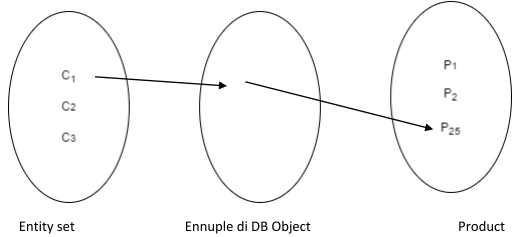
\includegraphics[scale=1]{figures/entity_setEV.png}
\caption{Entity Set Eulero-Venn} 
\end{figure}
\end{center}

La precedente descrizione del modello è stata estrapolata dal libro “Fundamentals of database systems”, mentre a lezione l’esempio si basava sulle entità Venditore e Prodotto. Il legame tra un’istanza di product e una di customer mi permette di ottenere una relazione che prende il nome di Tuple o ennupla. La tupla è una lista finita ordinata di elementi. Gli elementi di una tupla sono contenuti all’interno di “()”, ed ogni elemento 
è separata da una ”,”. Si comprende facilmente che gli elementi di una tupla sono gli attributi dell’entità presa in considerazione. Quindi, una relazione è un set di tuple degli oggetti del database. 
Gli attributi che hanno il ruolo di caratterizzare le entità e le relazioni possono essere definiti concettualmente:

\begin{itemize}

\item semplici;
\item composti;
\item multipli;
\item multipli \& composti.

\end{itemize}

Un attributo è semplice quando fornisce una singola informazione di base che caratterizza l’entità, assumendo un singolo valore (professione di una persona). Un attributo è composto quando è creato tramite l’uso di attributi semplici (l’indirizzo è composto dal tipo di via, nome della via, indirizzo civico, paese). Un attributo si dice multiplo quando a esso possono essere associati più valori dello stesso tipo contemporaneamente (locazione nel caso di un dipartimento universitario). Un esempio di attributo multiplo e composto è il numero di telefono, il quale è composto dal prefisso e dal numero. Durante la creazione di un database, tutti gli attributi composti e multipli devono essere convertiti in attributi semplici perché nei database relazionali sono accettati solo gli attributi semplici. 


\subsection{Come iniziare la progettazione di un DB}

Si parte con carta e penna, realizzando uno schema, non necessariamente corretto, in base alle richieste del committente. Solitamente non si riesce a creare un DB corretto subito. Vediamo un esempio.  
Il modello in figura evolve dinamicamente per ogni soluzione migliore che si riesce a trovare. 
Si è notato, in questo caso, che era più opportuno non considerare il nome del manager e la data di inizio del suo lavoro come attributo dell’entità department, ma creare una nuova entità di tipo impiegato che è in relazione con department.

\begin{center}
\begin{figure}[H]
\centering
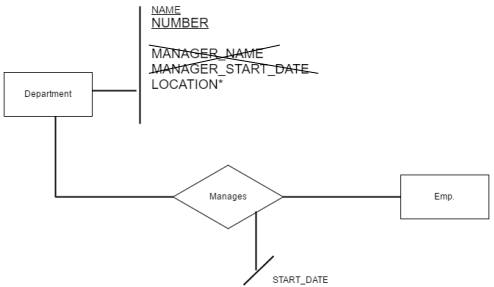
\includegraphics[scale=1]{figures/incER.png}
\caption{Incremental ER} 
\end{figure}
\end{center}

\subsection{Ternary relation type}

\begin{center}
\begin{figure}[H]
\centering
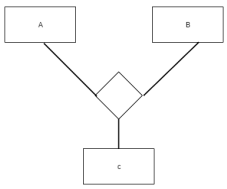
\includegraphics[scale=1]{figures/tER.png}
\caption{Ternary Relationship} 
\end{figure}
\end{center}

Nel caso in cui si ha la presenza di tre entità, in funzione della relazione usata, siamo in grado di estrapolare delle informazioni più precise. Per farlo si sfrutta una relazione ternaria, che diversamente da quella binaria, mette in collegamento attraverso una singola relazione tre entità. Le informazioni ottenute da una relazione ternaria contengono informazioni più precise rispetto a quando vengono usate delle relazioni binarie. Possiamo esprimere la precedente affermazione tramite disuguaglianza matematica: 

\[
	TernaryRelationship > BinaryRelationship
\]

\begin{center}
\begin{figure}[H]
\centering
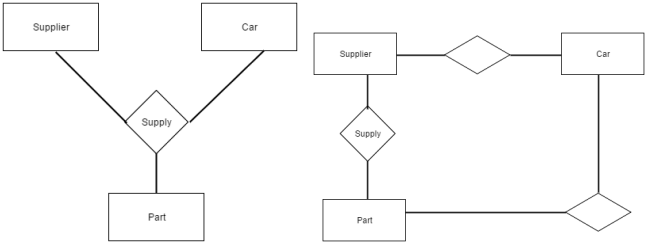
\includegraphics[scale=0.8]{figures/tER2.png}
\caption{Ternary Relationship and Three Binary Relationship} 
\end{figure}
\end{center}

Gli schemi rappresentati in figura sono equivalenti. Solo che, come già detto, 3 relazioni binarie contengono meno informazioni di una relazione ternaria. 
Per mantenere la stessa quantità di informazioni si fa uso della REIFICAZIONE, che consiste nel trasformare una relazione in un’entità. In questo modo si ha la presenza delle tre entità, un’entità reificata e tre relazioni binarie che collegano le entità all’entità reificata.  
Quindi continuo ad usare relazioni binarie anziché utilizzare relazioni ternarie, senza perdere informazione. 
In questo modo l’informazione estrapolata dalla relazione ternaria e l’informazione estrapolata dalla procedura di reieficazione è equivalente: 

\[
	TernaryRelationship := 3\ BinaryRelationShip + 1\ Entity Type
\]

L’uso di questa procedura è a discrezione esclusivamente del dal progettista. 

\begin{center}
\begin{figure}[H]
\centering
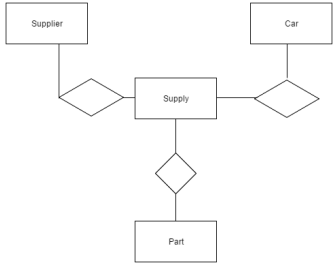
\includegraphics[scale=1]{figures/reification.png}
\caption{Reification of a Ternary Relationship} 
\end{figure}
\end{center}


\section{APPENDICE}

\subsection{DESIGN PATTERN}

Anche per i db esistono dei design pattern.

\begin{itemize}

\item{\textbf{\underline{X toX (es. Object type of object)}}} $\rightarrow$ Consiste nella distinzione tra oggetti unici, cioè rappresentati da un codice identificativo (automobile, armi, ...), e oggetti che sono istanze dello stesso tipo assolutamente identiche (capi di abbigliamento, generi alimentari, ...). Quindi la differenza consiste nel fatto che, si può acquistare, ad esempio, un’istanza di un oggetto (pacco di pasta) e non il singolo oggetto oppure il singolo oggetto se identificabile univocamente con qualche criterio. 
Questo pattern è utile in quanto è un tipico errore quello di inserire, all’interno del db, un oggetto al posto del tipo di oggetto.

\item{\textbf{\underline{Temporal Dimension}}} $\rightarrow$ Prima di dire lo scopo dell’utilizzo di questo pattern, è di fondamentale importanza rimarcare un concetto da tenere a mente quando si ha a che fare con il mondo dei DB, cioè che i dati sono fondamentali, sono importanti, sono una risorsa preziosa e a meno di casi eccezionali non vanno eliminati dal DB perché potrebbero ritornare utili in qualsiasi momento. Si sta facendo riferimento al concetto di Data Mining. ES. Se si dovessero perdere i dati (risorse immateriali) di una DB di una banca, che è un ente composto da risorse umane, materiali e immateriali, comporterebbe la perdita di tutte le informazioni relative ai correntisti o ai titoli bancari, di conseguenza le risorse materiali non avrebbero un possessore.  
Detto ciò, passiamo ad un esempio pratico per comprendere l’utilizzo di questo pattern.  Come si può vedere nella figura sottostante, il pattern Temporal Dimension esprime il fatto che alcuni attributi possano variare nel tempo, pertanto alle volte si ritiene opportuno avere uno storico delle informazioni, nel nostro caso variazioni di dati riguardanti il proprietario o 
l’automobile. In altre parole, sto aggiungendo la dimensione temporale al mio DB, per avere traccia delle varie versioni di un dato oggetto.   

\end{itemize}

\begin{center}
\begin{figure}[H]
\centering
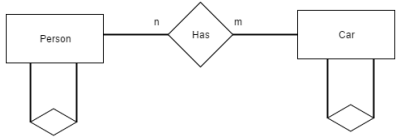
\includegraphics[scale=1]{figures/tdim.png}
\caption{Temporal Dimension} 
\end{figure}
\end{center}

\begin{flushright}Cristian Annicchiarico\\Mattia Marzano\\06/10/2016\end{flushright}


\section{Esercizio - Fermate Autobus}

I diagrammi Entità-Relazione (ER) sono stati estesi e migliorati con lo scopo di includere tecniche di modellazione tipiche del design object-oriented. Il risultato è una nuova classe di diagrammi definiti EER (Extended Entity-Relationship), che si avvicinano di più al concetto di diagramma delle classi UML. 

\textbf{Esercizio}: Siamo una compagnia di bus e vogliamo un’architettura del DB che ci aiuti a gestire il nostro business. Dobbiamo prendere in considerazione i seguenti punti:

\begin{itemize}

\item Bus;
\item Linee (fermate, collegamenti);
\item Impiegati;
\item Viaggiatori;
\item Biglietti (settimanali, mensili, annuali).

\end{itemize}

Gli aspetti precedenti sono ciò che chiamiamo \textbf{requisiti}, che il nostro progetto deve soddisfare. Alcune assunzioni aggiuntive verranno considerate nel prosieguo dell’esercizio in modo da ridurre la complessità del progetto. Senza perdita di generalità, considereremo solamente biglietti che sono validi in un lasso di tempo maggiore di 1 giorno (ovvero, settimanali/mensili/annuali), poiché i biglietti giornalieri non ci permettono di avere dettagli su chi stia usando quel biglietto, mentre, ad esempio, i biglietti settimanali richiedono una sorta di tessera che contiene i dati personali del viaggiatore. 

\textbf{Importante}: dobbiamo sempre ricordare che vogliamo un’architettura dei dati che soddisfi le esigenze di tutti i nostri stakeholder. In altre parole, il nostro design pattern è: Un database, multiple applicazioni (ovvero, interfacce e presentazioni differenti per gli stessi dati: vedi Figura 1). Anche se il database è lo stesso, utenti diversi usufruiscono di viste differenti degli stessi dati. Per spiegarlo attraverso un esempio, prendete un qualsiasi gioco di carte da tavolo: il database è “tutte le carte sul tavolo”, mentre ogni utente percepisce una diversa presentazione (infatti, lui o lei può solo sapere quali carte scoperte sono poste sul tavolo, quali carte sono nella sua mano, e quali carte erano nella sua mano).   

\begin{center}
\begin{figure}[H]
\centering
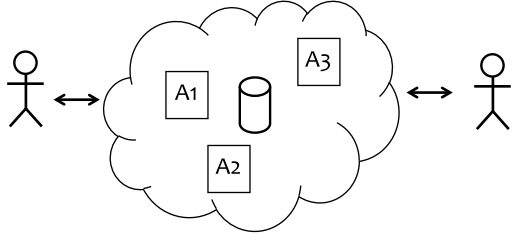
\includegraphics[scale=1]{figures/1DBmAPP.png}
\caption{Un database, multiple applicazioni} 
\end{figure}
\end{center}

Al fine di svolgere l’esercizio, consideriamo separatamente I requisiti. Prima di tutto, consideriamo le entità “Traveller” ed “Employee”. Al momento, modelliamole entrambe come un’unica entità “Person” con gli attributi appropriati:

\begin{center}
\begin{figure}[H]
\centering
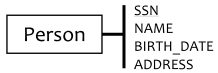
\includegraphics[scale=1]{figures/person_entity.png}
\caption{Entità "Person"} 
\end{figure}
\end{center}

Consideriamo ora linee con fermate e collegamenti. Questo ci porta alla creazione dell’entità “Line” (Figura 3).

\begin{itemize}

\item{\textbf{Domanda}}: dovremmo modellare le fermate di una certa linea come un attributo multiplo?
\item{\textbf{Risposta}}: No, poiché se consideriamo una fermata interposta tra due linee, dovremmo dichiararla due volte nel nostro database (ovvero, come un attributo sia della prima che della seconda linea). Questo violerebbe la terza regola dei database.

\end{itemize}

\textbf{Terza regola dei database}: Mai aggiungere ridondanza al vostro database! 

\textbf{Anticipazione}: In un diagramma E-R, la chiave primaria è solo concettuale (dobbiamo scegliere un campo che sia unico). Nella pratica, quando traduciamo un diagramma E-R nel suo corrispondente modello relazionale (modello logico), aggiungeremo un campo ID, responsabile dell’unicità di ciascuna entry nelle nostre tabelle. Esso sarà la nostra chiave primaria, ma non è visibile agli utenti. 

\begin{center}
\begin{figure}[H]
\centering
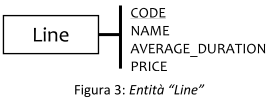
\includegraphics[scale=1]{figures/line_entity.png}
\caption{Entità "Line"} 
\end{figure}
\end{center}

Come specificare quali fermate attraversa una linea? Prima di tutto, dobbiamo modellare le fermate. Lo facciamo tramite un’entità “Stop”. 

\begin{center}
\begin{figure}[H]
\centering
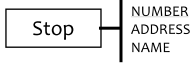
\includegraphics[scale=1]{figures/stop_entity.png}
\caption{Entità "Line"} 
\end{figure}
\end{center}

Come modellare i collegamenti tra le fermate? Abbiamo considerato varie alternative. Esaminiamole in ordine. 

\begin{itemize}

\item{\textbf{Prima alternativa per modellare le fermate}}

Poiché una linea è una sequenza di fermate, può essere considerata come una coda. Nei database, una coda può essere modellata creando una relazione ricorsiva (Figura 5). Comunque, questo approccio ha un problema. Prendete come esempio la Figura 6, in cui consideriamo due linee (rossa e verde). Nella linea rossa, la fermata blu è la numero 2, mentre nella linea verde, la fermata blu è la numero 3. Dovremmo modellare la fermata blu come la seconda o la terza fermata della coda? La risposta è: nessuna delle due, poiché la fermata blu deve comportarsi come terza fermata della coda per la linea rossa e come seconda fermata della coda per la linea verde. Con una simile architettura del database, come possiamo tenere traccia di quale fermata è situata a un certo punto di una certa linea? 

\begin{center}
\begin{figure}[H]
\centering
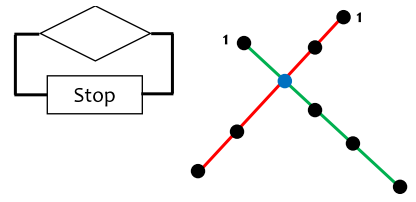
\includegraphics[scale=1]{figures/queue_stop.png}
\caption{A sx: Modellare una coda (prima alternativa), dx: Due line che condividono la stessa fermata} 
\end{figure}
\end{center}

\item{\textbf{Seconda alternative per modellare le fermate}}

Poiché il problema con la precedente soluzione era la mancanza di un collegamento tra la coda di fermate e le linee, un’idea sarebbe rimodellare lo scenario come mostrato in figura successiva. Comunque, questa architettura evidenzia due problemi: 

\begin{itemize}

\item E’ troppo complessa. Un requisito banale (una coda) non dovrebbe creare una grande complessità nel diagramma;
\item La relazione 1-1 tra “Queue” e “Line”, insieme con la totale partecipazione su entrambi i lati della relazione 1-1, suggerisce che di fatto “Queue” e “Line” siano lo stesso oggetto. Quindi, potremmo comprimerle in un’unica entità.   

\end{itemize}

\begin{center}
\begin{figure}[H]
\centering
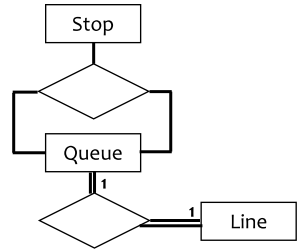
\includegraphics[scale=1]{figures/queue.png}
\caption{Modellare una coda (seconda alternativa)} 
\end{figure}
\end{center}

\item{\textbf{Terza alternative per modellare le fermate (la migliore)}}

Dopo tali considerazioni, abbiamo finito per semplificare la nostra architettura. La migliore alternativa (finora) è avere una semplice relazione N a M tra “Line” e “Stop” con un attributo \#Step che consente la creazione di una lista ordinata. E’ stato aggiunto un attributo addizionale Minutes, per modellare il tempo necessario, a partire dall’inizio di una corsa, per attraversare quella fermata. Inoltre, è un attributo multiplo, che dunque consente varie tempistiche per diverse ore della giornata. Lo scenario è riassunto nella successiva figura. Questa soluzione ha vari benefici:

\begin{itemize}

\item La complessità della ridefinizione della lista è spostata dentro all’applicazione. Quando una fermata è rimossa da una linea, deve essere eseguito da parte dell’applicazione il controllo di coerenza della lista;
\item Ha il giusto livello di complessità in paragone ai requisiti specificati;
\item Consente a un utente interessato di conoscere in che momento una linea attraversa una fermata: è sufficiente aggiungere il numero di minuti a partire dalla partenza del bus. 

\end{itemize}

\begin{center}
\begin{figure}[H]
\centering
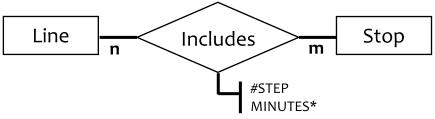
\includegraphics[scale=1]{figures/queue_final.png}
\caption{Modellare una coda (terza alternativa)} 
\end{figure}
\end{center}

\end{itemize}

Consideriamo ora il requisito dei biglietti. Non andremo a modellarlo come un’entità poiché significherebbe dire che i biglietti mensili esistono a prescindere dalla persona che li usa o a prescindere della linea per cui il biglietto è stato erogato. Questo ovviamente non è ciò che accade nella realtà. Motivo per cui modelleremo un biglietto come una relazione tra le entità interessate, come si può vedere dalla successiva figura. Questo è di fatto il modo più naturale di aggiungerlo nel nostro diagramma: un biglietto è un contratto, un pezzo di carta in cui sono scritte sia la persona che lo utilizza che la linea per cui può essere usato.

\begin{center}
\begin{figure}[H]
\centering
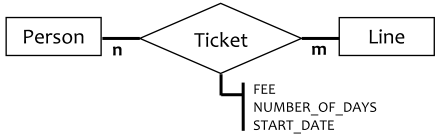
\includegraphics[scale=1]{figures/ticket_bus.png}
\caption{La relazione "Ticket"} 
\end{figure}
\end{center}

Infine, aggiungiamo il restante requisito al nostro diagramma: i bus. Prima di tutto, creiamo una nuova entità “Bus” (Prossima Figura). Abbiamo aggiunto alcuni attributi basilari, ma possiamo aggiungerne altri del tipo: numero di posti, se ha o meno supporto per persone disabili, se ha alcune utili agevolazioni per gli autisti, ecc..

\begin{center}
\begin{figure}[H]
\centering
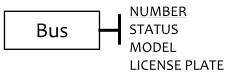
\includegraphics[scale=1]{figures/bus.png}
\caption{Entità "Bus"} 
\end{figure}
\end{center}

Ora dobbiamo analizzare due aspetti:

\begin{itemize}

\item Come modellare la tabella oraria per le linee?
\item Come tener traccia di quale bus ha servito una certa linea in un certo giorno a una certa ora?  

\end{itemize}

Per rispondere alla prima domanda, abbiamo introdotto l’entità “Race” (Successiva figura). Questa nuova entità debole modella una particolare istanza di una linea (con una tabella oraria). Mentre “Line” indica un percorso teorico attraverso alcune fermate, “Race” è una particolare istanza di “Line” che ha un orario di partenza formale per ogni giorno della settimana. 

\begin{center}
\begin{figure}[H]
\centering
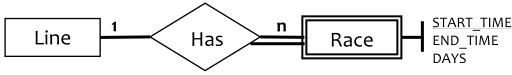
\includegraphics[scale=1]{figures/race_line.png}
\caption{Entità “Race” e suo collegamento all’entità “Line”} 
\end{figure}
\end{center}

Con questa nuova entità, la seconda domanda può essere riformulata nel seguente modo: come tener traccia di quale bus ha servito una certa corsa? Questo può essere banalmente ottenuto aggiungendo una relazione tra “Race” e “Bus” (Successiva figura). Il diagramma ER finale è riportato in Figura 13. Comunque, questa impostazione non considera chi ha guidato in una certa corsa. Non abbiamo esplorato questo punto nella lezione, ma può essere ottenuto in vari modi:

\begin{itemize}

\item Modificando la relazione “Served” in successiva figura in una relazione ternaria, in cui il terzo collegamento è attaccato all’entità “Person”;
\item Aggiungendo una relazione tra “Person” e “Race” (ma questo obbliga gli impiegati a guidare sempre nella stessa corsa e non permette modifiche negli assegnamenti).

\end{itemize}

\begin{center}
\begin{figure}[H]
\centering
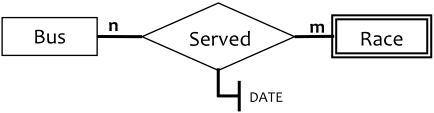
\includegraphics[scale=1]{figures/served.png}
\caption{La relazione “Served”} 
\end{figure}
\end{center}

\newpage
\begin{center}
\begin{figure}[H]
\centering
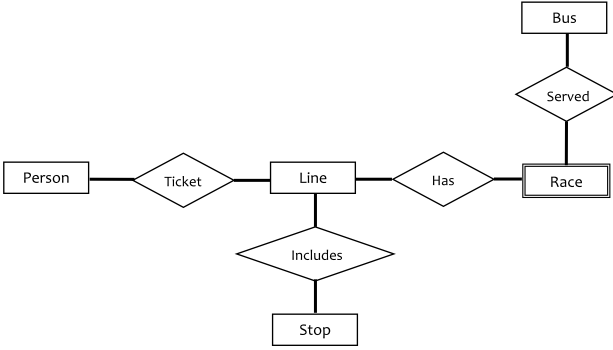
\includegraphics[scale=0.8]{figures/finalbusER.png}
\caption{Diagramma ER finale per l’esercizio sulla compagnia di bus} 
\end{figure}
\end{center}
\newpage

Le fermate dovrebbero essere collegate alle corse? Introduciamo un altro design pattern che risolve questo problema: il Preventivo Consuntivo. Questo ci consentirà di salvare l’informazione circa il tempo effettivo in cui una corsa ha attraversato una certa fermata in un certo giorno (permettendoci, ad esempio, di ricalcolare periodicamente il tempo di arrivo stimato sulla base delle statistiche).

\subsection{Design Pattern: Preventivo-Consuntivo}

Questo pattern gestisce la previsione di un evento e la sua effettiva realizzazione. Introduciamolo tramite un esempio: la prenotazione in un hotel. La previsione è la prenotazione di una camera, mentre la realizzazione è ciò che accade effettivamente (ovvero, se la camera viene occupata o meno al tempo previsto). In questo caso, possono accadere tre situazioni: 

\begin{itemize}

\item Qualcuno prenota la camera e la usa (prenotazione + uso);
\item Qualcuno prenota la camera ma non la usa (prenotazione + non uso);
\item Nessuno prenota la camera ma qualcuno la usa (no prenotazione + uso).

\end{itemize}

Di fatto possono accadere più situazioni (per esempio, vi potrebbero essere multiple prenotazioni e cancellazioni, o una prenotazione per N persone e $N \neq M$ persone che la usano, ecc…) Se il diagramma originario contiene una relazione tra due entità A e B (ad esempio “Person” e “Room”) che è di tipo Preventivo-Consuntivo (ad esempio “Books” e “Uses”), questo pattern richiede di dividere la relazione in due relazioni: prevenire (Books) e consumare (Uses). Questa situazione è illustrata nella successiva figura:

\begin{center}
\begin{figure}[H]
\centering
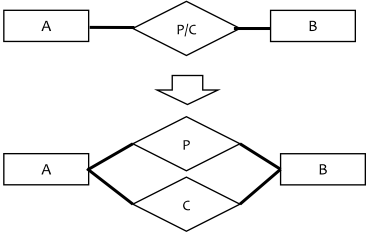
\includegraphics[scale=1]{figures/prevcon.png}
\caption{ Divisione della relazione. P e C stanno rispettivamente per Prevenire e Consumare} 
\end{figure}
\end{center}

Nell’esempio di prenotazione di un hotel, con tale architettura è possibile avere informazioni separate circa la prenotazione di camera e l’utilizzo di camera. Comunque, c’è ancora un tassello mancante: la relazione tra Preventivo e Consumazione (ovvero, quale consumazione ha seguito quale preventivo). Nondimeno, nel nostro esempio ciò non è un problema, poiché può esistere solo un utilizzo alla volta per una specifica camera: la relazione tra P e C può essere facilmente ricostruita. Se è richiesta una specifica relazione tra P e C, la si può ottenere ridefinendo le relazioni P e C (Successiva figura). Questa struttura è più forte ma davvero complessa. Nel nostro esempio di prenotazione, ciò ci consentirebbe di conoscere quale prenotazione è stata seguita da un effettivo utilizzo. In altre parole, ci permetterebbe di sapere che una certa prenotazione è quella che ha di fatto consentito a una persona di entrare e utilizzare la camera prenotata. Consumazione = un’attuazione di un’azione preventiva. 

\subsection{Conclusione}

 Abbiamo specificato molti requisiti. Ciascuno di essi ha avuto impatto sulla soluzione finale. Dovremmo controllare costantemente se essi sono soddisfatti e coperti dalla nostra soluzione. Inoltre, dobbiamo sempre essere pronti a suggerire altre soluzioni quando sono richieste. L’Informazione è un’ecosistema di Produttori, Consumatori e Trasformatori.
 
\textbf{N.B.}: Non dobbiamo ottimizzare il nostro database per le query, ma per gli stakeholder (deve soddisfare appropriatamente ciascuno di essi). 

\begin{center}
\begin{figure}[H]
\centering
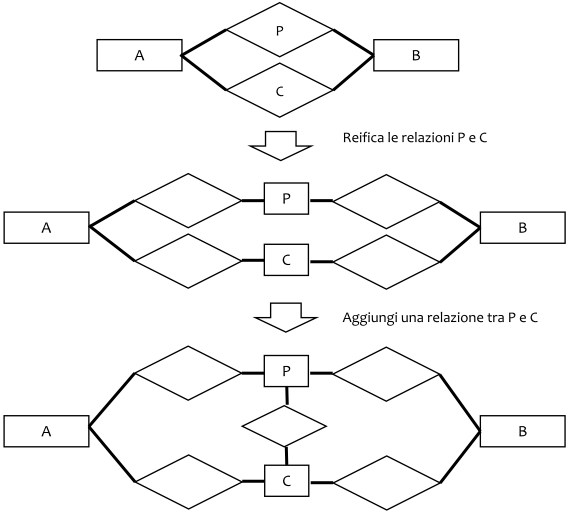
\includegraphics[scale=1]{figures/prevconEXP.png}
\caption{ Divisione della relazione. P e C stanno rispettivamente per Prevenire e Consumare} 
\end{figure}
\end{center}

\begin{flushright}Andrea Camisa\\Gioele Sforza\\6/10/2016\end{flushright}

\section{DATA CENTRIC APPLICATION}

La lezione di oggi ha lo scopo di analizzare il ciclo di creazione e modellazione di applicazioni che si occupano di database. Per l’ingegneria delle applicazioni Data Centric si utilizza un approccio differente: 

\underline{MAPPING ALGORITHM} Trasforma i diagrammi E.R. in tabelle relazionali:

\begin{itemize}

\item{\underline{CONCEPTUAL MODEL}} (ER DIAGRAM);
\item{\underline{LOGICAL MODEL}} – RELATIONAL MODEL (Concetti Astratti);   
\item{\underline{PHYSICAL MODEL}} (REAL DATABASE – MySQL).

\end{itemize}

Un database è un insieme di relazioni $R_i$ e vincoli $C_j$:

\[
	DB = \{R_i,\ C_j\}
\]

Le relazioni sono le tabelle, i vincoli sono le regole che gestiscono le tabelle. Ci sono dei livelli per la costruzione di un database: 

\begin{itemize}

\item{\textbf{PRESENTATION LAYER – P.L.}};
\item{\textbf{BUSINESS RULE LAYER – B.R.L.}};
\item{\textbf{DATABASE LAYER – D.L.}};

\end{itemize}

\subsection{USER TYPES}

Gli User Types sono gli agenti che estraggono le informazioni da Database in modo differente utilizzando il medesimo software. Per ognuno di essi bisogna progettare quindi diverse interfacce e diverse regole di accesso al DB:

\begin{center}
\begin{figure}[H]
\centering
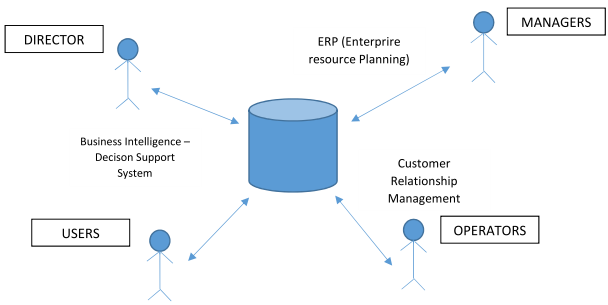
\includegraphics[scale=0.8]{figures/ut.png}
\caption{User Types} 
\end{figure}
\end{center}

\subsection{ESEMPIO}

Usiamo un’applicazione esempio per analizzare lo schema appena spiegato (DL, BRL, PL):

\begin{center}
\begin{figure}[H]
\centering
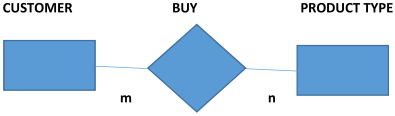
\includegraphics[scale=1]{figures/cbuypt.png}
\caption{Customer Buys Product Type} 
\end{figure}
\end{center}

In questo esempio gli UserTypes sono i Customers e i Sellers e sono per lo più statici, cioè non cambiano. Mentre i Product Type sono più dinamici in quanto rapprensentano le transazioni economiche. 

\begin{center}
\begin{figure}[H]
\centering
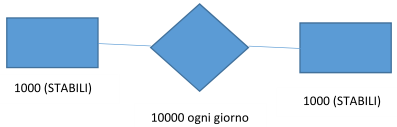
\includegraphics[scale=1]{figures/cbuypt_alim.png}
\caption{Customer Buys Product Type - Dinamicità} 
\end{figure}
\end{center}

$\leftarrow$ La dinamicità della relazione è molto più alta rispetto alle altre due entità. Come facciamo a estrarre differenti info per le diverse tipologie di users? Si userà una forma semplificata del \textbf{Mapping Algorithm}.

\subsection{SIMPLIFIED MAPPING ALGORITHM}

\begin{itemize}

\item \textbf{Ogni Entity Type diventa una tabella e i loro attributi diventano i nomi delle colonne}. Customer, products diventano tabelle, con i relativi attributi. Ogni customer diventerà un record della tabella Customer:

\begin{center}
\begin{figure}[H]
\centering
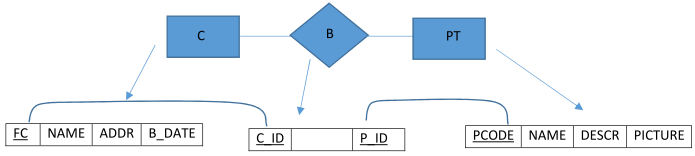
\includegraphics[scale=0.8]{figures/cbuypt_mapping.png}
\caption{Customer Buys Product Type - Mapping} 
\end{figure}
\end{center}

\item \textbf{Ogni Relation Types diventa una tabella}. E’ sempre vero in un solo caso, ovvero quando la relazione è “molti a molti” (n:m):

\begin{itemize}

\item \textbf{Collegare la chiave esterna (F.K.) a ogni entità};
\item \textbf{Completare la tabella con tutti gli attributi presenti della Relation Type}.

\end{itemize}

\begin{itemize}

\item Nel caso \textbf{n:m} si crea quello che si chiama \textbf{Relational Schema of DB};

\item Nel caso della relazione \textbf{1:n}, bisogna includere la tabella della relazione nella tabella finale  dell’entità “\textbf{n}” 

\begin{center}
\begin{figure}[H]
\centering
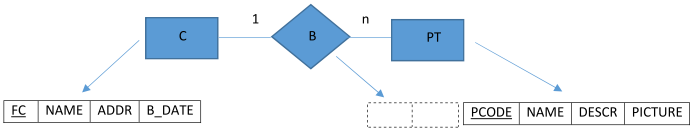
\includegraphics[scale=0.8]{figures/cbuypt1n_mapping.png}
\caption{Customer Buys Product Type - 1:n Mapping} 
\end{figure}
\end{center}

\item Nel caso della relazione \textbf{1:1} si può includere la tabella della relazione in una delle due entità oppure creare una sola tabella:

\begin{center}
\begin{figure}[H]
\centering
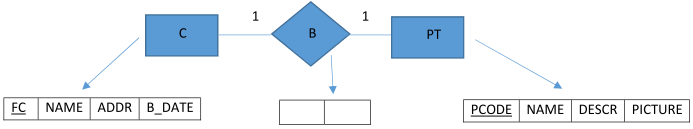
\includegraphics[scale=0.8]{figures/cbuypt11_mapping.png}
\caption{Customer Buys Product Type - 1:1 Mapping} 
\end{figure}
\end{center}

\end{itemize}

\end{itemize}

Se cancello un record da una tabella entità, verrà cancellato ogni record relativo presente nella tabella relazione. Il discorso non vale tra tabelle entità diverse, poiché indipendenti tra loro. Riferendoci all’esempio precedente se ad esempio viene cancellato un customer, ogni transazione riferita a lui viene cancellata, lo stesso vale per i prodotti.  

\subsection{PRESENTATION LAYER FOR CUSTOMER OR DIRECTOR}

Avremo differenti livelli di presentazione, uno per il customer e uno per il direttore del negozio. Per il Customer la Web Application si vedrà come:

\begin{center}
\begin{figure}[H]
\centering
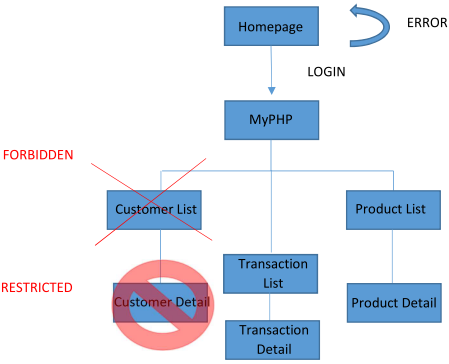
\includegraphics[scale=1]{figures/plcd.png}
\caption{\textbf{Navigation Model of a Website For Customer}}
\end{figure}
\end{center}

Un’altra soluzione potrebbe essere: 

\begin{center}
\begin{figure}[H]
\centering
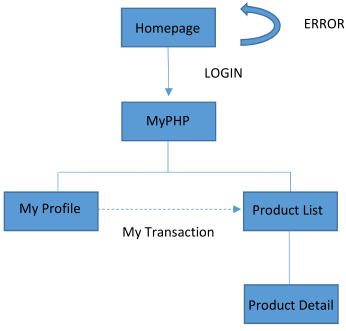
\includegraphics[scale=1]{figures/plcd2.png}
\caption{\textbf{Navigation Model of a Website For Customer} - Another solution}
\end{figure}
\end{center}

Per il Director invece, la Web Application si vedrà come: 

\begin{center}
\begin{figure}[H]
\centering
\includegraphics[scale=1]{figures/pld.png}
\caption{\textbf{Navigation Model of a Website For Director}}
\end{figure}
\end{center}

Il direttore ha la possibilità di creare o cancellare i prodotti e di modificare gli attributi di essi. Inoltre può ottenere informazioni sui Customers e quindi potrà poi effettuare delle scelte strategiche per migliorare le vendite con pubblicità o sconti mirati. 

\subsection{BUSINESS RULE LAYER}

Man mano che si sale nella piramide abbiamo bisogno di aggregare le informazioni fino ad avere delle info sempre più riassuntive.

Quando si realizza un progetto c’è bisogno di definire: 

\begin{itemize}

\item CONTEXT \& PROBLEM DEFINITION (2 PAGINE);
\item GOAL \& STAKEHOLDERS;
\item REQUIREMENTS \& CONSTRAINTS;  
\item DATA MODEL:

\begin{itemize}

\item ER DIAGRAM;
\item RELATIONAL MODEL;
\item PHYSICAL MODEL.

\end{itemize}

\item SYSTEM MODELS;
\item SOFTWARE MODELS (MODEL VIEW CONTROLLER):

\begin{itemize}

\item STATE MODEL;
\item PRESENTATION MODEL:

\begin{itemize}

\item IN THE LARGE NAVIGATION (Modello per mostrare le pagine e le connessioni fra di esse);
\item IN THE SMALL NAVIGATION (Modello per analizzare ogni aspetto singolarmente);
\end{itemize}
\end{itemize}
  
\item TEST MODEL;
\item DEPLOYMENT STRATEGY.

\end{itemize}

\section{LIST VIEW and DETAIL VIEW}

Questi due concetti provengono dai sistemi operativi (WINDOWS, MACOS, XWINDOWS/UNIX) e nascono dall’idea comune detta WIMP INTERFACE:

\begin{itemize}

\item WINDOWS = Diversi spazi di lavoro per diverse operazioni (MULTITASKING);
\item ICONS = Oggetti Interattivi;
\item MENUS = Metodi associati ai propri oggetti;
\item POINTERS = Selezionare un oggetto specifico.

\end{itemize}

Da questa metafora nasce l’idea di LIST VIEW e DETAIL VIEW. Se ad esempio apro il Desktop ottengo una lista di oggetti, se invece interagisco con uno di essi ottengo informazioni dettagliate. 

\begin{itemize}

\item{\textbf{LIST VIEW}}

List View può essere una tabella nella quale sono presenti dei metodi well-known come:

\begin{itemize}

\item DELETE OBJECT;
\item SORT;
\item (MOVE);
\item COPY (DUPLICATE OBJECT);
\item INSERT EMPTY OBJECT;
\item FILTER;
\item RENAME;
\item SEARCH (FIND).

\end{itemize}

Altri esempi di List View possono essere una Cartina Geografica, il Desktop o una cartella, un Sets o un Tree. 

\item{\textbf{DETAIL VIEW}}

I metodi well-known della Detail View possono essere:

\begin{itemize}

\item CHANGE (UPDATE);
\item CREATE;
\item DELETE;
\item READ.

\end{itemize}

\end{itemize}

\begin{flushright}Angelo Cotardo\\Francesco Filieri\\12/10/2016\end{flushright}

\begin{center}
\begin{figure}[H]
\centering
\includegraphics[scale=1]{figures/dbut.png}
\caption{Database and User Types}
\end{figure}
\end{center}

Continuiamo con una discussione più dettagliata riguardo i design patterns. Nella scorsa lezione abbiamo esplorato l’intera catena che inizia dal modello e termina con le applicazioni. Il database è un luogo in cui differenti tipi di utente possono svolgere molteplici azioni, ognuno di essi è collegato a qualche processo, descritto tramite un linguaggio grafico chiamato BPML (Business Process Modeling Language) che descrive i processi in un’organizzazione. 
Parleremo di BUSINESS MODEL, molto importante per i nostri scopi, di DATA MODEL, usato per il database e infine di PRESENTATION MODEL e SYSTEM MODEL. 
Quando parliamo di CONCEPTUAL MODEL, ci riferiamo a tutti i modelli che sono molto usati per raccogliere requisiti e informazioni riguardo a ciò che è necessario fare e per trasformare poi questi in software. Approfondiremo gli aspetti di data modeling. 
Abbiamo già introdotto il concetto di ER che andremo ad espandere con i design patterns e con il concetto di EER (ENHANCED ENTITY RELATIONSHIP). Aggiungeremo poi anche qualche concetto riguardo la modellazione di oggetti (ereditarietà ecc.). 

\subsection{DATA PATTERN}

\textbf{Introduciamo il concetto di DATA PATTERN}

Consideriamo il seguente schema:

\begin{center}
\begin{figure}[H]
\centering
\includegraphics[scale=1]{figures/cbuyp.png}
\caption{Customer Buys Product Provided By Provider}
\end{figure}
\end{center}

Stiamo considerando lo scenario in cui un consumatore compra dei prodotti, i quali sono forniti da più fornitori. Osservando gli attributi delle relazioni e delle entità descritte, oltre alla quantità, al tipo di prodotto acquistato e alla data di acquisto, si è definito l’attributo “price” che compare per ben tre volte come attributo delle due relazioni e dell’entità PRODUCT. 

Il significato che assume tale attributo cambia: 

\begin{itemize}

\item{\textit{Selling cost}};
\item{\textit{Catalog cost}};
\item{\textit{Payed cost}}.

\end{itemize}

Nel primo caso esprime il costo del prodotto appena comprato, nel secondo si riferisce al prezzo specificato nel catalogo dei prodotti (non necessariamente selling price deve essere uguale al catalog price ) e nel terzo caso ci si riferisce al prezzo pagato al fornitore riguardo quel prodotto, il quale ovviamente è diverso dal prezzo specificato nel catalogo. 
Il pattern che si è applicato in questo caso (cioè trovare lo stesso attributo in entità o relazioni differenti) prende il nome di PRICE CHAIN (o più in generale ATTRIBUTE CHAIN). 
Un altro tipo di pattern che presentiamo è il PRESENTATION PATTERN che non si focalizza sui dati, bensì sulla loro rappresentazione: l’ARCHIVE PATTERN. È collegato al concetto che quando memorizziamo delle informazioni, esse possono diventare col tempo poco usate.

\begin{center}
\begin{figure}[H]
\centering
\includegraphics[scale=1]{figures/interest_lvl.png}
\caption{Interest Level for Objects}
\end{figure}
\end{center}

Dallo schema si può notare i vari livelli di interesse (LI) per ogni elemento inserito in una list view (cioè le informazioni contenute in tali elementi). In alcuni sistemi quindi, più di un elemento può avere lo stesso livello di interesse, in altri invece, come quelli usati da Google per le ricerche, le informazioni in cima alla lista avranno un livello di interesse elevato rispetto ai successivi elementi. 
Per gestire ciò, viene assegnato ad ogni query un ranking, cioè un indicatore in base al quale ordinare i risultati. Quindi le “risposte” con informazioni più recenti alle “domande” effettuate avranno un ranking più elevato rispetto alle altre. Tali indicatori possono essere assegnati ad esempio sulla base del numero di persone interessate ad un determinato argomento. Un altro esempio del genere, non più basato sul concetto di ranking, può essere quello di una email software, in cui le email più vecchie sono meno importanti delle ultime ricevute, pertanto ci si basa sul tempo.  
Un esempio in cui tutti gli elementi possono avere lo stesso livello di interesse può essere quello dei contatti Whatsapp, in cui ad ognuno di essi viene data la stessa importanza:

\begin{center}
\begin{figure}[H]
\centering
\includegraphics[scale=1]{figures/whatsapp_rd.png}
\caption{Whatsapp: Receiving Date attribute}
\end{figure}
\end{center}

Possiamo aggiungere a tale entity type un \textbf{ranking attribute} (o altri tipi di attributi che collegano il livello di attenzione ai dati). In questo caso consideriamo l’attributo RECEIVING DATE per produrre un archivio gerarchico: 

\begin{center}
\begin{figure}[H]
\centering
\includegraphics[scale=1]{figures/hierarchical_rd.png}
\caption{Whatsapp: Schema gerarchico costruito sulla base dell'attributo Receiving Date}
\end{figure}
\end{center}

Considerando il caso di una email software, si possono organizzare le email ricevute per categorie: anni, mesi, settimane, giorni ecc. Si mette quindi più attenzione alle email ricevute di recente rispetto alle più vecchie (viene assegnato un ranking basato sul tempo). 

\subsubsection{EXAMPLE}

consideriamo il seguente scenario 

\begin{center}
\begin{figure}[H]
\centering
\includegraphics[scale=1]{figures/pppbuy.png}
\caption{Relazione ternaria con PART, PROJECT, PROVIDER}
\end{figure}
\end{center}

Possiamo decidere di usare una relazione ternaria perché tre relazioni binarie non sono sufficienti per dire che una parte specifica è stata fornita da uno specifico fornitore ad uno specifico team (o project).  
Una relazione ternaria quindi collega i tre oggetti nello stesso tempo, cosa che non succederebbe se usassimo tre relazioni binarie. Per dimostrare che la quantità di informazioni è variata possiamo usare il concetto di reificazione. Per trasformare una relazione abbiamo infatti bisogno di un nuovo schema in cui compaiono tre relazioni binarie più una nuova entità (PROVISIONING): 

\begin{center}
\begin{figure}[H]
\centering
\includegraphics[scale=1]{figures/ppp_extended.png}
\caption{Reificazione della Relazione ternaria con PART, PROJECT, PROVIDER}
\end{figure}
\end{center}

Per verificare la cardinalità delle partecipazioni di ogni entità alla relazione ternaria, focalizziamo il nostro punto di vista su ciascuna di esse, vedendo le parti rimanenti del DB come una coppia. 
Ad esempio, concentrandoci sull’entità PART la relazione con la coppia (PROJECT, PROVIDER) è di tipo a molti (n), in quanto ci sono più parti che possono essere fornite da differenti fornitori per differenti progetti. Nello stesso modo, concentrandoci sull’entità PROJECT e osservando la relazione con la coppia (PART, PROVIDER), si nota che in un progetto si possono utilizzare più parti diverse da diversi fornitori, pertanto si assegna una relazione a molti (m). Nel caso del PROVIDER la relazione è di tipo a molti (p), perché si possono vedere una o più coppie del tipo (PART, PROJECT). 
Bisogna tener presente che una volta effettuata la reificazione la cardinalità non varia.                           

Supponiamo di avere due entity type con la seguente cardinalità:  

\begin{center}
\begin{figure}[H]
\centering
\includegraphics[scale=1]{figures/cbuyp2.png}
\caption{Customer Buys Product}
\end{figure}
\end{center}

Trasformando tale schema si ricaveranno tre tabelle, due per le entità e un’altra per la relazione (in quanto si ha una cardinalità n:m). Considerando la seguente variante derivata dalla reificazione:

\begin{center}
\begin{figure}[H]
\centering
\includegraphics[scale=1]{figures/cbuyp_checkout.png}
\caption{Enhanced Customer Buys Product}
\end{figure}
\end{center}

si è trasformato la relazione BUY nell’entità SHOPPING SESSION che può essere effettuata da un cliente e che può includere più prodotti. Dal punto di vista delle informazioni potremmo anche chiamare tale entità con il nome di BILL O TICKET, ma non è propriamente corretto in quanto non è un oggetto esistente, ma solo una collezione di informazioni di altri oggetti. 
Tale entità è il risultato della reificazione e non dall’analisi del problema, per tale motivo questa entità si può considerare come una “entity type di seconda classe” perché non è realmente una classe autonoma dalle altre. Una buona modellazione è considerare tale entity type come una weak entity con un proprio customer. 
Il concetto generale di weak entity type è un po’ differente da quello adottato in questo caso, perché un’entità del genere non può essere identificata in modo univoco dai suoi soli attributi, ma dalla primary key dell’entità collegata ad essa, cioè quella del customer (esempio: due notebook identici sono perfettamente uguali nei loro attributi, ciò che li distingue è il proprietario a cui appartengono). 
In questo caso la SHOPPING SESSION differisce in parte dal concetto di entity type dal momento che possiede anche attributi riguardanti il ticket number e la data del ticket, pertanto ha già delle sue informazioni caratteristiche (la sua primary key che la identifica). 
Infine un CUSTOMER può avere più SHOPPING SESSION, ma ciascuna di esse può avere solo un CUSTOMER e pertanto la relazione a molti (n) dello schema di partenza diventa 1:n. D’altra parte una SHOPPING SESSION può includere più prodotti come anche più prodotti possono essere inclusi in più SHOPPING SESSION facendo diventare la relazione a molti (m) una relazione n:m. Quindi la cardinalità dello schema ER di partenza è legata a quella specificata dopo la reificazione. Gli attributi della relazione di partenza diventeranno gli attributi dell’entità derivata dalla reificazione.  

\subsubsection{EXERCISE: PHR (EHR)}

\begin{center}
\begin{figure}[H]
\centering
\includegraphics[scale=1]{figures/phr.png}
\caption{Personal Health Record (PHR)}
\end{figure}
\end{center}

(proviamo ad usare PRICE CHAIN e ARCHIVE PATTERN) 
Questo problema è chiamato PHR (Personal Health Record) (Cartella Sanitaria Elettronica): il paziente si reca dal medico di famiglia, viene informato circa la sua situazione clinica e gli vengono prescritti alcuni test da fare. Il paziente si reca al centro dei test clinici (CTL), oppure in ospedale (H, PH) per radiografie o per altri test. Successivamente i risultati verranno consegnati al medico di famiglia. Questo è uno scenario classico.  
Perché non creare un database online di pazienti, così da mettere tutti i loro report e accedere alle informazioni usando solo username e password? Il problema è abbastanza semplice da descrivere, ma è abbastanza complesso da risolvere. Google creò alcuni anni fa Google Health e Microsoft presentò Microsoft Healthvault, due applicazioni che permettevano di inserire tutte le nostre informazioni nel database. Google e Microsoft hanno realizzato questi database e hanno fallito. Adesso non ci sono soluzioni disponibili in questo ambito.   

Possibili problemi in cui si può incorrere sono:

\begin{itemize}

\item persone anziane;
\item no standard;
\item benefits misunderstanding (i pazienti non comprendono i benefici);
\item i dottori non vogliono l’automazione (power knowledge);
\item aspetti legati alla privacy.

\end{itemize}

Il fallimento di tali sistemi sta anche nel fatto che potremmo essere “bombardati” da tanti annunci riguardanti alcuni specifici rimedi. Se qualcuno pagasse, potrebbe forzare Google a dare informazioni false riguardo la nostra salute. Inoltre le preoccupazioni relative alla privacy sono estremamente importanti e l’interesse economico del mondo dei dati personali della salute è di decine di miliardi di euro. 

\textbf{Analizziamo i requisiti del database di una clinica}.

Quando il paziente arriva in clinica, la receptionist lo ammette e informa il dottore che è arrivato un paziente (è una ammissione tecnica, gli permette l’ingresso). Il dottore a sua volta ammette il paziente che sta aspettando, questa è un’ammissione clinica, perché dal punto di vista medico un dottore dice al paziente che può iniziare una cura/terapia. Il paziente quindi descrive il problema e il dottore fa l’anamnesi (scrive le note e mette tutte le informazioni nella cartella del paziente, nel sistema). I dottori sottoscrivono la prescrizione, i test e invitano i pazienti a sottoporsi ad essi (anche nella stessa clinica). Successivamente delle infermiere effettuano i test e i risultati sono poi inseriti nel sistema. I pazienti potranno visualizzare i risultati dei test a casa sul loro computer.  
Elenchiamo i tipi di utente presenti nello scenario descritto:

\begin{itemize}

\item DOCTOR;
\item RECEPTIONISTS;
\item PATIENTS;
\item NURSES.

\end{itemize}

Descriviamo lo scenario mediante questo semplice schema: 

\begin{center}
\begin{figure}[H]
\centering
\includegraphics[scale=1]{figures/clinics_req.png}
\caption{Clinics - Requirements}
\end{figure}
\end{center}

Possiamo vedere quanto facile e immediato è descrivere un problema in termini di dati scambiati tra i tipi di utente. Il framework che abbiamo visto è molto efficace perché iniziamo a vedere ciò che ci circonda in modo differente. Ci sono: tipi di utente, azioni, informazioni (che sono scambiate tra i vari utenti), tipi di relazioni tra entità. Abbiamo così una buona e immediata descrizione di un problema reale. 

Iniziamo una prima fase di modellazione considerando tre relazioni binarie tra le seguenti entità: 

\begin{center}
\begin{figure}[H]
\centering
\includegraphics[scale=1]{figures/clinics_ER.png}
\caption{Clinics - ER Draft}
\end{figure}
\end{center}


\begin{flushright}Andrea Cuna\\Giuseppe Levantaci\\13/10/2016\end{flushright}

Riprendiamo la modellazione del problema della clinica. Sono sicuramente necessarie le seguenti entity type:

\begin{itemize}

\item PATIENT;
\item DOCTOR;
\item RECEPTIONIST. 

\end{itemize}

Dobbiamo tener conto del fatto che un paziente prenota in anticipo una visita. Quando egli si presenta in ambulatorio, dovrà essere “ammesso” alla visita dal receptionist, il quale ovviamente “informerà” il medico: 

\begin{center}
\begin{figure}[H]
\centering
\includegraphics[scale=1]{figures/clinics_incER.png}
\caption{Clinics - Incremental ER}
\end{figure}
\end{center}

Vediamo ora come specificare l’intervista del dottore al paziente:

\begin{center}
\begin{figure}[H]
\centering
\includegraphics[scale=0.8]{figures/pid.png}
\caption{Doctor Interviews Patient}
\end{figure}
\end{center}

Va ricordato, ora, che le interviste riguardano la storia clinica del paziente, lo stile di vita e il problema medico attuale, e l’assunzione o meno di farmaci, per cui avremo le seguenti relazioni:

\begin{itemize}

\item Il paziente è connesso ad altri pazienti da una relazione (ricorsiva) di parentela (informazione utile per considerare l'eventuale ereditarietà delle malattie): 

\begin{center}
\begin{figure}[H]
\centering
\includegraphics[scale=1]{figures/pirof.png}
\caption{Patient Is Relative Of Patient}
\end{figure}
\end{center}

\item Il paziente è malato:

\begin{center}
\begin{figure}[H]
\centering
\includegraphics[scale=1]{figures/patient_has_disease.png}
\caption{Patient Has Disease}
\end{figure}
\end{center}

\item Il paziente assume medicinali:

\begin{center}
\begin{figure}[H]
\centering
\includegraphics[scale=1]{figures/patient_assume_drug.png}
\caption{Patient Assume Drug}
\end{figure}
\end{center}

\item Ora inseriamo il concetto di stile di vita del paziente (ad esempio se è un fumatore) modellando una nuova entity type: 

\begin{center}
\begin{figure}[H]
\centering
\includegraphics[scale=1]{figures/patient_has_lb.png}
\caption{Patient Has Lifestyle Behavior}
\end{figure}
\end{center}

\end{itemize}

Come si può vedere, queste ultime quattro relazioni tengono traccia delle informazioni che scaturiscono dall’intervista.	

Vediamo ora come si può modellare la prescrizione di medicine, esami, test e indagini cliniche al paziente da parte del dottore:

\begin{itemize}

\item Si potrebbe modellare in questo modo:

\begin{center}
\begin{figure}[H]
\centering
\includegraphics[scale=1]{figures/doctor_prescribe_drug.png}
\caption{Patient Has Lifestyle Behavior}
\end{figure}
\end{center}

\item Potremmo considerare anche: 

\begin{center}
\begin{figure}[H]
\centering
\includegraphics[scale=1]{figures/patient_rpa_drug.png}
\caption{Patient Receives Prescription About Drug}
\end{figure}
\end{center}

\end{itemize}

Ora sappiamo che durante la visita il dottore prescrive le medicine al paziente, inoltre l’intervista è qualcosa che avviene durante la visita. Per questo è possibile applicare la reificazione a VISIT e assumere che durante la visita il paziente dichiari di usare medicine e di avere un certo stile di vita; in questo modo non sarà più necessario specificare la data dell’intervista come attributi delle due relazioni HAS, e si terrà anche conto del dottore.   

\begin{center}
\begin{figure}[H]
\centering
\includegraphics[scale=0.8]{figures/clinics_incER2.png}
\caption{Clinics - Incremental ER 2}
\end{figure}
\end{center}

In precedenza abbiamo detto che durante l'intervista (e quindi durante la visita), il paziente comunica al dottore le medicine che assume, il dottore prescrive al paziente delle medicine e gli diagnostica una malattia. Queste considerazioni ci permettono di associare DISEASE e DRUG a VISIT, invece che a PATIENT.	

In questo modo le relazioni precedenti diventano: 

\begin{center}
\begin{figure}[H]
\centering
\includegraphics[scale=0.8]{figures/clinics_incER3.png}
\caption{Clinics - Incremental ER 3}
\end{figure}
\end{center}

In seguito ad una visita, il medico potrebbe anche prescrivere al paziente un “esame”, il quale verrà effettuato da un “infermiere”, quindi possiamo modellare in questo modo:   

\begin{center}
\begin{figure}[H]
\centering
\includegraphics[scale=1]{figures/clinics_incER4.png}
\caption{Clinics - Incremental ER 4}
\end{figure}
\end{center}

In particolare, NURSE effettua un TEST (nel senso di un esame specifico di un determinato paziente) di tipo TYPE OF TEST (inteso come esame in senso generico, ad esempio “analisi del sangue”), il quale è prescritto da un medico (stiamo utilizzando il pattern Object-Type of object). 
Abbiamo bisogno dunque delle seguenti relation types:

\begin{itemize}

\item DOES (NURSE-DOES-TEST);
\item INSTANCE OF (TEST-INSTANCE OF-TYPE OF TEST);
\item PRESCRIBES (VISIT-PRESCRIBES-TYPE OF TEST).

\end{itemize}
	
La prescrizione del test si può modellare, dunque, in questo modo:

\begin{center}
\begin{figure}[H]
\centering
\includegraphics[scale=0.8]{figures/clinics_incER5.png}
\caption{Clinics - Incremental ER 5}
\end{figure}
\end{center}

\newpage
Il modello ER finale per il nostro problema è il seguente: 

\begin{center}
\begin{figure}[H]
\centering
\includegraphics[scale=0.8]{figures/clinics_finalER.png}
\caption{Clinics - Final ER}
\end{figure}
\end{center}


\section{DBMS}

\subsection{Descrizione dei principali DBMS}

\begin{center}
\begin{figure}[H]
\centering
\includegraphics[scale=0.8]{figures/DBMS.png}
\caption{DBMS}
\end{figure}
\end{center}

Tra i DBMS più conosciuti troviamo:  

\begin{itemize}

\item MySQL;
\item MongoDB;
\item SQLite;
\item PostgreSQL;
\item Oracle;
\item Microsoft SQL Server;
\item Microsoft Access (e il suo competitor OpenOffice Base);
\item Couchbase.

\end{itemize}

Analizziamone alcuni più in dettaglio. 

\begin{itemize}

\item{\textbf{Oracle, Microsoft SQL Server} e \textbf{MySQL}} sono RDBMS, ovvero DBMS “\textbf{relazionali}” (che coprono circa il 90 \% del mercato dei DBMS). Oracle ha un prezzo di circa 60.000 €, SQL Server 10.000 €, mentre MySQL è gratuito, pur essendo in qualche modo paragonabile agli altri due. Oracle e SQL Server sono di fascia “enterprise”, impiegati quindi nell’ambito di grandi aziende (es. banche), mentre MySQL è perfetto per gli studenti universitari che si affacciano al mondo dei database;

\item{\textbf{MongoDB} e \textbf{Couchbase}} sono DBMS “NoSQL”, ovvero NON relazionali, idonei per particolari applicazioni;

\item{\textbf{PostgreSQL}} è un Object Relational DBMS, ovvero presenta alcune caratteristiche tipiche della programmazione orientata agli oggetti. Questo consente un Object-Relational Mapping più preciso;

\item Infine, \textbf{Microsoft Access} e il suo diretto competitor open source \textbf{OpenOffice Base} sono semplici DBMS utilizzati principalmente per la costruzione veloce di prototipi di database.

\end{itemize}


\subsection{Installazione e configurazione di MySQL} 

\begin{itemize}

\item{\textit{Installazione su Microsoft Windows}}

Recarsi al seguente indirizzo: \url{http://dev.mysql.com/downloads/mysql/}; Selezionare il proprio Sistema Operativo ed eseguire il Download.

\begin{center}
\begin{figure}[H]
\centering
\includegraphics[scale=0.8]{figures/mySQLinstaller.png}
\caption{MySQL Installer Download}
\end{figure}
\end{center}

Prima di effettuare l’installazione eseguire il seguente download:

\begin{center}
\begin{figure}[H]
\centering
\includegraphics[scale=0.8]{figures/visualc++.png}
\caption{Visual C++ Redistributable Packages download}
\end{figure}
\end{center}

Dopo il download selezionare ed avviare l’installazione, il file avrà nome: \newline “ mysql-installercommunity-x.x.x.x-dmr.msi “ dove x.x.x.x sarà il numero di versione, verrà poi visualizzata la seguente schermata:

\begin{center}
\begin{figure}[H]
\centering
\includegraphics[scale=1]{figures/mySQLinstaller_splash.png}
\caption{MySQL Installer Splash-Screen}
\end{figure}
\end{center}

Verrà visualizzata la seguente schermata: 

\begin{center}
\begin{figure}[H]
\centering
\includegraphics[scale=0.8]{figures/mySQLinstaller_wizard.png}
\caption{MySQL Installer Wizard}
\end{figure}
\end{center}

Accettare i termini di licenza e poi proseguire nell’installazione. 

Nella schermata successiva selezionare quanto evidenziato: 

\begin{center}
\begin{figure}[H]
\centering
\includegraphics[scale=1]{figures/mySQLinstaller_wizard2.png}
\caption{MySQL Installer Wizard 2}
\end{figure}
\end{center}

E nella schermata successiva configurare i pacchetti come riportati in figura: 

\begin{center}
\begin{figure}[H]
\centering
\includegraphics[scale=1]{figures/mySQLinstaller_wizard3.png}
\caption{MySQL Installer Wizard 3}
\end{figure}
\end{center}

e quindi proseguire nell’installazione cliccando due volte sul tasto “ Next $>$ “. Si raggiungerà la seguente schermata:

\begin{center}
\begin{figure}[H]
\centering
\includegraphics[scale=0.8]{figures/mySQLinstaller_wizard4.png}
\caption{MySQL Installer Wizard 4}
\end{figure}
\end{center}

Al termine dell’installazione verrà installato, oltre al server, il software “MySQL WorkBench” il quale è utile per creare e gestire le tabelle dei database contenuti nel server. Al primo avvio del server verrà richiesto di inserire una password di amministratore: qui si può inserire una password a scelta che dovrà essere ricordata per eseguire l’accesso negli usi successivi. 

\item{\textit{INSTALLAZIONE SU MACOS}}

Recarsi allo stesso URL indicato in precedenza, selezionare il sistema operativo MacOS ed eseguire il download del pack dmg. In seguito, una volta aperto il pack dmg ed avviata l’installazione del pack pkg al suo interno, si otterrà questa schermata:

\begin{center}
\begin{figure}[H]
\centering
\includegraphics[scale=1]{figures/mySQLinstaller_macOS_wizard.png}
\caption{MySQL Installer MacOS Wizard}
\end{figure}
\end{center}

cliccando su continua si dovrà poi accettare la licenza:

\begin{center}
\begin{figure}[H]
\centering
\includegraphics[scale=1]{figures/mySQLinstaller_macOS_wizard2.png}
\caption{MySQL Installer MacOS Wizard 2}
\end{figure}
\end{center}

Successivamente nella schermata successiva basterà cliccare su “Installa” e verrà avviata l’installazione durante la quale sarà richiesta la password di amministratore: 

\begin{center}
\begin{figure}[H]
\centering
\includegraphics[scale=1]{figures/mySQLinstaller_macOS_wizard3.png}
\caption{MySQL Installer MacOS Wizard 3}
\end{figure}
\end{center}

Alla fine dell’installazione verrà visualizzata una finestrella contenente la password di amministratore generata automaticamente: 

\begin{center}
\begin{figure}[H]
\centering
\includegraphics[scale=1]{figures/mySQLinstaller_macOS_wizard4.png}
\caption{MySQL Installer MacOS Wizard 4}
\end{figure}
\end{center}

Dopo di che sarà possibile avviare il Server tramite le impostazioni:

\newpage

\begin{center}
\begin{figure}[H]
\centering
\includegraphics[scale=1]{figures/macOS_mySQL_settings.png}
\caption{Mac OS Settings MySQL}
\end{figure}
\end{center}

\begin{center}
\begin{figure}[H]
\centering
\includegraphics[scale=1]{figures/mySQL_serverstatus.png}
\caption{MySQL Server Status}
\end{figure}
\end{center}
\newpage

Ora bisogna installare “MySQL WorkBench”: Eseguire il download da questo link: \url{http://dev.mysql.com/downloads/workbench/}. Seguendo i passaggi riportati sopra per la selezione del sistema operativo. Una volta eseguito il download aprire il pack dmg ottenendo: 

\begin{center}
\begin{figure}[H]
\centering
\includegraphics[scale=1]{figures/mySQL_workbench_splash.png}
\caption{MySQL Workbench Splash-Screen}
\end{figure}
\end{center}

E come suggerisce l’immagine, spostare l’applicazione nella cartella per eseguire l’installazione.

\end{itemize}

\subsection{PRIMO CONTATTO CON MYSQL WORKBENCH}

Aprire il programma. Si troverà la seguente schermata:

\begin{center}
\begin{figure}[H]
\centering
\includegraphics[scale=0.8]{figures/mySQL_workbench_home.png}
\caption{MySQL Workbench Home Screen}
\end{figure}
\end{center}

Cliccando sul “+” accanto a MySQL Connections si potrà aggiungere una nuova connessione ad un database SQL già avviato ( vedi passaggi precedenti ) visualizzando una schermata che chiederà di inserire la password da amministratore:  

\begin{center}
\begin{figure}[H]
\centering
\includegraphics[scale=1]{figures/mySQL_login.png}
\caption{MySQL Login Screen}
\end{figure}
\end{center}

Una volta eseguito l’accesso, si avrà la seguente schermata: 

\begin{center}
\begin{figure}[H]
\centering
\includegraphics[scale=0.8]{figures/mySQL_workbench_initial.png}
\caption{MySQL Workbench Initial Screen}
\end{figure}
\end{center}

Tramite il tasto “ Server Status“ è possibile visionare lo stato del server e “Avviare/Fermare” l’istanza del server SQL:

\begin{center}
\begin{figure}[H]
\centering
\includegraphics[scale=0.8]{figures/mySQL_workbench_serverstatus.png}
\caption{MySQL Workbench Server Status}
\end{figure}
\end{center}

Tramite il tasto “+” posizionato a destra della scritta Models in basso a sinistra:  
si potrà creare un nuovo modello, visualizzando la seguente schermata:  

\begin{center}
\begin{figure}[H]
\centering
\includegraphics[scale=0.8]{figures/mySQL_workbench_model.png}
\caption{MySQL Workbench - Model}
\end{figure}
\end{center}

Cliccando su “Add Table” ( evidenziato nella figura precedente ) si potrà inserire una nuova tabella nel nostro modello e la schermata diventerà: 

\begin{center}
\begin{figure}[H]
\centering
\includegraphics[scale=0.8]{figures/mySQL_workbench_addtable.png}
\caption{MySQL Workbench - Add Table}
\end{figure}
\end{center}

In basso al centro verrà visualizzata la struttura della nuova tabella. Tramite “Name” sarà possibile rinominarla. Costruire una tabella come quella riportata in figura:  

\begin{center}
\begin{figure}[H]
\centering
\includegraphics[scale=0.8]{figures/mySQL_workbench_newtable.png}
\caption{MySQL Workbench - New Table}
\end{figure}
\end{center}

in cui:

\begin{itemize}

\item{\textbf{id}} è la CHIAVE PRIMARIA (PK) NON NULLA (NN) e AUTO INCREMENTANTE (AI) identificata come un intero;
\item{\textbf{first\_name} e \textbf{last\_name}} sono Nome e Cognome della persona identificati come un insieme di stringhe di massimo 45 caratteri;
\item{\textbf{birth\_date}} è la data di nascita della persona ed è identificato come un oggetto DATE (ossia una data in formato internazionale AAAA-MM-GG);
\item{\textbf{picture}} è invece l’immagine di una persona identificata nel database con un oggetto BLOB ossia un Binary Long OBject;

\end{itemize}

Ora in alto nei menù si dovrà selezionare : “ Database $\rightarrow$ Forward Engineering ” per eseguire il salvataggio del nostro modello sul server a cui siamo collegati, tramite questo semplice wizard: 

\begin{center}
\begin{figure}[H]
\centering
\includegraphics[scale=1]{figures/mySQL_workbench_FE.png}
\caption{MySQL Workbench - Forward Engineering}
\end{figure}
\end{center}

qui va selezionato il server di destinazione, in seguito selezionare le opzioni necessarie (per ora lasciamo tutto invariato) 

\begin{center}
\begin{figure}[H]
\centering
\includegraphics[scale=0.8]{figures/mySQL_workbench_FE2.png}
\caption{MySQL Workbench - Forward Engineering step 2}
\end{figure}
\end{center}

Poi bisognerà selezionare gli oggetti che si vogliono ottenere da questa esportazione:

\begin{center}
\begin{figure}[H]
\centering
\includegraphics[scale=1]{figures/mySQL_workbench_FE3.png}
\caption{MySQL Workbench - Forward Engineering step 3}
\end{figure}
\end{center}

Verrà mostrato il codice SQL di creazione del modello prima di essere esportato sul server: 

\begin{center}
\begin{figure}[H]
\centering
\includegraphics[scale=0.8]{figures/mySQL_workbench_FE4.png}
\caption{MySQL Workbench - Forward Engineering step 4}
\end{figure}
\end{center}

Infine si esegue il salvataggio:

\begin{center}
\begin{figure}[H]
\centering
\includegraphics[scale=1]{figures/mySQL_workbench_FEfinal.png}
\caption{MySQL Workbench - Forward Engineering - Save}
\end{figure}
\end{center}

Andando ora a rivedere il contenuto del server (sempre tramite il Workbench) troveremo un nuovo database chiamato \textbf{mydb}:

\begin{center}
\begin{figure}[H]
\centering
\includegraphics[scale=0.8]{figures/mySQL_workbench_mydb.png}
\caption{MySQL Workbench - mydb RECAP}
\end{figure}
\end{center}

cliccando col tasto destro sulla tabella \textbf{person} e selezionando: “ Select Row – Limit 1000 ” verrà visualizzato il contenuto della tabella caricata sul server con la seguente schermata: 

\begin{center}
\begin{figure}[H]
\centering
\includegraphics[scale=0.8]{figures/mySQL_workbench_person.png}
\caption{MySQL Workbench - person set on server}
\end{figure}
\end{center}

dove nella parte in alto viene visualizzata la “QUERY”, e in basso il risultato (ovviamente ora viene visualizzata una tabella vuota). A questo punto fare doppio click nella selezione rossa nell’immagine, in corrispondenza di first\_name, e inserire il nome. Continuare così per il resto dei campi e poi premere invio, in questo modo si inseriranno i dati all’interno della tabella. Bisognerà ottenere un risultato come il seguente: 

\begin{center}
\begin{figure}[H]
\centering
\includegraphics[scale=1]{figures/mySQL_workbench_personinsert.png}
\caption{MySQL Workbench - Insert new people}
\end{figure}
\end{center}

In seguito in basso a sinistra si troverà il tasto “Apply”:

\begin{center}
\begin{figure}[H]
\centering
\includegraphics[scale=0.8]{figures/mySQL_workbench_apply.png}
\caption{MySQL Workbench - Apply}
\end{figure}
\end{center}

Si aprirà il seguente wizard in cui sarà visualizzata la QUERY da eseguire sul database:

\begin{center}
\begin{figure}[H]
\centering
\includegraphics[scale=0.8]{figures/mySQL_workbench_prequerywizard.png}
\caption{MySQL Workbench - Pre-query wizard}
\end{figure}
\end{center}

Cliccando su “Apply” verrà eseguita la query ottenendo il seguente risultato: 

\begin{center}
\begin{figure}[H]
\centering
\includegraphics[scale=1]{figures/mySQL_workbench_postscriptwizard.png}
\caption{MySQL Workbench - Post-query wizard}
\end{figure}
\end{center}

Provare ora ad eseguire le QUERY:

\begin{itemize}

\item{}

\begin{lstlisting}[language=SQL]
SELECT * FROM mydb.person WHERE first_name = 'Mario'
\end{lstlisting}

\item{}

\begin{lstlisting}[language=SQL]
SELECT * FROM mydb.person WHERE first_name = 'M'
\end{lstlisting}

\item{}

\begin{lstlisting}[language=SQL]
SELECT * FROM mydb.person WHERE first_name = 'mario'
\end{lstlisting}

\end{itemize}

e proseguire facendo varie prove, modificando le QUERY. 

\begin{flushright}Marco D'Amato\\Marco Mameli\\13/10/2016\end{flushright}


\section{IMPORTANZA MODELLI}

\subsection{IMPORTANZA MODELLO DATI}

Tra i vari modelli dell’ingegneria del software, il modello dati ha una rilevanza particolare in quanto influisce in maniera determinante sulle funzionalità dell’applicazione. Tuttavia, i vari schemi di un sistema software sono:

\begin{itemize}

\item{DATABASE MODEL}: come già accennato, il più importante;
\item{BUSINESS MODEL}: vagamente simile al diagramma dei casi d’uso, ha il compito di esplicare le ragioni presenti dietro lo sviluppo di un sistema software. Consiste nella creazione di scenari, nei quali i prodotti applicativi servono a creare delle soluzioni a problemi specifici. Questi schemi mostrano lo scambio di valore intorno all’applicazione (E3 VALUE);
\item{MODELLO DI SISTEMA}: importante per la scalabilità e la realizzabilità dell’applicazione;

\item{PRESENTATION MODEL}: in questo caso si parla di visibility design, dove i vari attori sono inseriti in un diagramma in cui sono riportate le varie funzioni relative ad ognuno di essi.

\begin{center}
\begin{figure}[H]
\centering
\includegraphics[scale=1]{figures/cbuyp3.png}
\caption{Customer Buys Product}
\end{figure}
\end{center}

Ultimamente quello dei disappearing computer è uno dei più interessanti ambiti di ricerca, dove per computer si intendono smart devices e smart processes: l’obiettivo è quello di rendere smart la parte relativa all’inserimento e al rilevamento dati;

\item{TEST}: relativamente meno importante degli altri, ma validi da un punto di vista economico in quanto spesso è il collaudo a sbloccare i finanziamenti per il software. 
 
\end{itemize}

\subsection{IMPORTANZA INFORMAZIONE}

\begin{center}
\begin{figure}[H]
\centering
\includegraphics[scale=1]{figures/dmo.png}
\caption{Anthony's DMO Pyramid}
\end{figure}
\end{center}

Nella progettazione di un sistema software è importante progettare interfacce diverse per tipo di utente, creando diagrammi di comunicazione on the large per ogni utente. 

\begin{center}
\begin{figure}[H]
\centering
\includegraphics[scale=1]{figures/otl.png}
\caption{On the Large Communication Diagram}
\end{figure}
\end{center}

Esempio sui canali di comunicazione:

\begin{itemize}

\item Lettori leggono prodotto Autori;
\item Autori leggono feedback dei Lettori;
\item Lettori leggono feedback degli altri Lettori (casi generici Booking.com, TripAdvisor);
\item Community di Autori. 

\end{itemize}

\section{DIAGRAMMI EER}

Le tre caratteristiche della progettazione ad oggetti sono: Ereditarietà, Polimorfismo, Incapsulamento. Quest’ultimo non è presente nei Database, in quanto le entità non sono trasparenti; il polimorfismo è una componente essenziale per la programmazione, mentre non lo è per i dati. Per aggiungere l’Ereditarietà ai diagrammi E-R (Entity-Relationship) sono stati introdotti i diagrammi EER (Enhanced Entity Relationship).

\begin{center}
\begin{figure}[H]
\centering
\includegraphics[scale=1]{figures/EER.png}
\caption{Diagramma EER}
\end{figure}
\end{center}

La modifica apportata allo schema di riferimento Cliente - Acquista - Prodotto rappresenta la specializzazione dell’entità cliente (si noti il simbolo di inclusione insiemistica). A questo punto si presentano due possibili situazioni:

\begin{itemize}

\item

\begin{center}
\begin{figure}[H]
\centering
\includegraphics[scale=1]{figures/EERset1.png}
\caption{Diagramma di Eulero-Venn per EER disjoint entities}
\end{figure}
\end{center}

Le due entità pur essendo incluse nell’entità parent, non hanno elementi in comune. In questo caso si dicono disgiunte, e nel cerchio presente nel simbolo di specializzazione del diagramma EER si inserisce la lettera “d” (disjoint):

\begin{center}
\begin{figure}[H]
\centering
\includegraphics[scale=1]{figures/disjoint.png}
\caption{Disjoint Inheritance for EER}
\end{figure}
\end{center}

\item

\begin{center}
\begin{figure}[H]
\centering
\includegraphics[scale=1]{figures/EERset2.png}
\caption{Diagramma di Eulero-Venn per EER overlapping entities}
\end{figure}
\end{center}

Le due entità potrebbero avere elementi in comune, come nel caso sotto riportato. In tal caso si inserisce la lettera “o” (overlap):

\begin{center}
\begin{figure}[H]
\centering
\includegraphics[scale=1]{figures/overlapping.png}
\caption{Overlapping Inheritance for EER}
\end{figure}
\end{center}

\end{itemize}

Esiste un importante differenza tra specializzazione e generalizzazione: La prima, effettuata a priori è sempre possibile, mentre la seconda non sempre. Nell’ultimo caso si può scoprire a posteriori che oggetti diversi appartengono alla stessa classe rendendo difficile per il software aggiornare la struttura dati. Un modo fattibile di implementare la generalizzazione è attraverso la UNION. Tale elemento di modellazione concettuale è rappresentato come sotto, dove in tal caso si inserisce il simbolo di “u” (union):

\begin{center}
\begin{figure}[H]
\centering
\includegraphics[scale=0.8]{figures/union.png}
\caption{Union for EER}
\end{figure}
\end{center}

A differenza dell’Overlap, in questo caso le entità child mantengono i loro attributi ma sono unite sotto l’entità parent risolvendo parzialmente il problema: infatti nel caso della union si ha che fare con insiemi di oggetti diversi aventi attributi diversi. Si noti che l’entità Vehicle non contiene niente tranne che l’ID che però non è presente a livello concettuale ma solo a livello logico (dove sono presenti le tabelle). 

\subsection{SCHEMA EER CAPITOLO 4} 

\begin{center}
\begin{figure}[H]
\centering
\includegraphics[scale=0.7]{figures/EERschema_cpt4.png}
\caption{\textbf{SCHEMA EER CAPITOLO 4}}
\end{figure}
\end{center}

Nel diagramma sopra riportato la doppia linea rappresenta una specializzazione esclusiva, a indicare una partecipazione totale.  Le due diverse specializzazioni disgiunte sono entrambe ortogonali, in quanto le entità child sono indipendenti l’una dall’altra. Nel caso di ereditarietà multipla non sempre le speciali portano ad alberi aperti: come si evince dal precedente diagramma possono esserci maglie chiuse. Il caso peggiore di queste situazioni si presenta quando gli attributi vengono gestiti due volte, anche se si tratta di un evento abbastanza raro.


\subsection{ESERCIZIO SVOLTO IN CLASSE}

\begin{center}
\begin{figure}[H]
\centering
\includegraphics[scale=0.7]{figures/museum.png}
\caption{\textbf{Museum Exercise ER}}
\end{figure}
\end{center}


\begin{flushright}Ippazio Alessio\\Simone Dongiovanni\\19/10/2016\end{flushright}

%************************************************
% Chapter 2: MODELLO LOGICO
%************************************************
% !TEX encoding = UTF-8
% !TEX TS-program = pdflatex
% !TEX root = ../nt.tex
% !TEX spellcheck = it-IT

%************************************************
\chapter{MODELLO LOGICO}
\label{cap:logical}
%************************************************\\

\section{SQL QUERY: Le interrogazioni del database}

Per effettuare un'interrogazione del database bisogna avere una procedura sistematica che, dato un problema, ci consente di trovare una soluzione e verificarla in diversi casi di test in modo da appurare che sia una soluzione generale e non particolare.  

\underline{Esempio}: Una lista di clienti è una query sull'entità di tipo di cliente, ma non ci basta una sola query perché avremmo bisogno di vedere i clienti in ordine di nome, di luogo, di residenza, di data di nascita, ecc.   

\begin{center}
\begin{figure}[H]
\centering
\includegraphics[scale=0.8]{figures/cliente_acquista_prodotto.png}
\caption{Cliente Acquista Prodotto} 
\end{figure}
\end{center}

Le query devono rispondere ottimamente qualunque sia il criterio di filtraggio e devono essere robuste: ad esempio esiste la possibilità di, non conoscendo username e password, ma inserendo righe di codice in modo opportuno, poter entrare in un database (SQL INJECTION). Bisogna quindi fare attenzione nel momento in cui si scrive una query perché qualcuno potrebbe iniettarvi dei pezzi aggiuntivi. La connessione tra le pagine e il database avviene attraverso un certo numero di query: questo codice deve essere robusto, verificato, sviluppato attraverso procedure precise e rigorose basate sul concetto dell'algebra relazionale. 

Le query sono formule matematiche scritte in algebra relazionale. Il modo migliore per scrivere  una query è capire l'algebra che c'è dietro. 

\begin{center}
\begin{figure}[H]
\centering
\includegraphics[scale=0.8]{figures/cap_logical.png}
\caption{Cliente Acquista Prodotto - Mapping} 
\end{figure}
\end{center}

Uno schema viene trasformato in tabella in base al tipo di cardinalità della relazione. Queste tabelle d'ora in poi saranno chiamate relazioni. L'algebra relazionale è un'algebra insiemistica in cui  gli insiemi sono rappresentati non da diagrammi di Venn, ma da tabelle, in questo senso si dice  che un database è un insieme di relazioni $(R_i)$ e vincoli o constraints $(C_j)$:

\[
	DB = \{R_i,\ C_j\}
\]

I vincoli sono una serie di regole che utilizzeremo per far sì che i nostri dati restino coerenti,  cioè che il database resti un database. Le caratteristiche principali sono: assenza di ridondanza, minima quantità di NULL, unicità di rappresentazione dell'informazione, ecc.  
L'oggetto di base dell'algebra relazionale, come detto, è la relazione o tabella. Oltre alle relazioni abbiamo un certo numero di operatori: come nell'algebra ci sono i numeri $\{1,2,3,\ \dots\}$ e li combiniamo attraverso operatori $\{+,*,\ \dots\}$, così in quella relazionale esistono operatori unari e binari. Un ulteriore modello è quello dell'algebra booleana dove  esistono operatori unari e binari (ad esempio l'operatore \textit{not} applicato ad un bit 0 fornisce  come risultato 1, mentre \textit{and} applicato a 1 fornisce 0).  


\subsection{ALGEBRA RELAZIONALE}

Tutte le tabelle che vengono fuori dall'algebra relazionale sono calcolate, cioè vengono  create come il risultato di un'espressione, pertanto sono solo viste, non vengono memorizzate  e non occupano spazio. 

\begin{itemize}

\item{\textbf{Operatori Unari}}:

Per quanto riguarda gli operatori unari dell'algebra relazionale: 

\begin{itemize}

\item Il primo tra tutti gli operatori che ci interessano è quello di “\textit{select}”. Si scrive come: 

\[
	\sigma_{<c>}(R)
\]

Questo operatore estrae o seleziona dalla tabella R una nuova tabella fatta dalle stesse colonne della tabella R e dalle sole righe che soddisfano la condizione C (fare riferimento cap. 4 e cap. 8 del libro).

\underline{Esempio} Seleziona $\sigma_{<CLIENT.CITY="LECCE">}(CLIENT)$. Cosa viene fuori da questa espressione? Avremo una nuova tabella chiamata R avente le stesse colonne della tabella clienti e un sottoinsieme delle righe;


\item Il secondo operatore è “project”, così come la select riduce il numero di righe, la project riduce il numero di colonne estraendone solo alcune. Si scrive come:

\[
	\pi_{<col1,\ col2,\ \dots>}(R)
\]

Questo operatore prende un numero selezionato o ridotto delle colonne della tabelle di  partenza;

\item Il terzo operatore è “\textit{rename}”, serve a rinominare determinati attributi. Questo produce una nuova tabella in cui le colonne si chiamano in un altro modo. Si scrive come: 

\[
	\rho_{col1\ as\ new1,\ col2\ as\ new2,\ \dots}(R)
\]

\end{itemize}

\item{\textbf{Operatori Binari}}:

Il secondo gruppo di operatori sono di tipo insiemistico. Questi richiedono che gli oggetti siano  union-compatible, cioè che abbiano le stesse colonne o che si chiamino nella stessa maniera.  Le operazioni che conosciamo sono: 

\begin{itemize}

\item{Unione}: denotata con $R \cup S$. Posso fare quest'operazione solo se la prima e la seconda tabella hanno le stesse colonne, ciò è garantito dalla union-compatible. Lo loro unione è una nuova tabella virtuale in cui ci sono tutte le righe della prima tabella e tutte quelle della seconda;

\item{Intersezione}: denotata con $R \cap S$. Se ho due righe con gli stessi nomi di colonna,  fare l'intersezione degli elementi presenti sia in R che in S significa selezionare gli elementi comuni. La chiave primaria deve garantire che ogni riga sia univocamente definita dato che la teoria dell'algebra relazionale dice che tutti i dati devono essere diversi;

\item{Differenza}: denotata con $R-S = R-(R\cap S)$. È il set di tutti gli elementi che sono inclusi in R ma non in S;

\item{Prodotto cartesiano}: $R \times S$.  Questa operazione genera l'insieme di tutte le possibili coppie $T\{(r_i,s_j)\}$ Immaginiamo che R ed S siano dei concetti o idee, la capacità di creare corrispondenze tra queste genera dei nuovi concetti applicativi. Si intuisce, però, che l'insieme di tutte le coppie possibili è troppo grande (alcune non hanno senso e non servono), perciò eliminiamo le connessioni inutili utilizzando l'operazione di join;

\item{Join}:

\[
	R \Join S := \sigma_{<c>}(R \times C)
\]

Essa è l'operazione chiave dei database. È ciò che facciamo quando scriviamo \textit{SELECT FROM WHERE}. La selezione è la possibilità di estrarre solo alcune colonne da una tabella potendo esprimere la condizione. In altre parole fare la join di due tabelle dal punto di vista dell'algebra relazionale significa attaccare tutti gli elementi corrispondenti. 

\end{itemize}

\underline{Esempio}: Join di due tabelle:

\begin{center}
\begin{figure}[H]
\centering
\includegraphics[scale=0.8]{figures/join.png}
\caption{Join di due tabelle} 
\end{figure}
\end{center}

Questa notazione senza righe è ciò che d'ora in poi chiameremo \underline{modello relazionale} (insieme di tabelle più insieme di vincoli), in cui specifichiamo i vincoli di chiave primaria (sottolineata), di chiave esterna $(ID\_c)$ e vincoli di integrità referenziale (freccia).

\end{itemize}

\subsection{Operatore Join}

Analizziamo l'operatore join attraverso uno scenario: supponiamo di avere Mario Rossi  con indirizzo Lecce e Giorgio Bianchi con indirizzo Milano, nel nostro autosalone abbiamo  la macchina 1 che è una Fiat Tipo che ha il prezzo di € 10mila. Inizialmente nel DB non c'è scritto nulla ma nel momento in cui viene venduta ci aggiungiamo le informazioni riguardanti Mario Rossi con la data di acquisto. Fare il prodotto cartesiano delle due tabelle significa avere tutte  le combinazioni o coppie possibili. Se adesso ci facciamo sopra una selezione sulla condizione di join, cioè vogliamo selezionare solo le righe $Prodotto.ID_c = Cliente.ID_c$ vedremo solo le coppie che soddisfano la corrispondenza.   

\begin{center}
\begin{figure}[H]
\centering
\includegraphics[scale=0.8]{figures/cliente_prodotto_logical.png}
\caption{Scenario logico Cliente/Prodotto} 
\end{figure}
\end{center}

La join è una nuova tabella, che per il momento indichiamo come Cliente-Prodotto, contenente tutte le colonne del cliente $\{c_1, c_2, c_3,\ \dots\}$ e tutte le colonne del prodotto $\{p_1, p_2, p_3,\ \dots\}$ che soddisfano  la condizione di join, ovvero che la chiave esterna di una tabella deve essere uguale alla corrispondente chiave primaria dell'altra tabella (se non ho venduto nessuna macchina la tabella di join sarà vuota).  

\begin{center}
\begin{figure}[H]
\centering
\includegraphics[scale=0.8]{figures/cliente_join_prodotto.png}
\caption{Cliente JOIN Prodotto} 
\end{figure}
\end{center}

In algebra relazionale l'operazione di join è scritta in questo modo: 

\[
	Cliente \Join_{<Prodotto.ID=Cliente.ID_c>}(Prodotto)
\]

Unire le tabelle significa prendere le coppie degli elementi corrispondenti. Come si scrive questa cosa all'interno di una select? Possiamo ad esempio scrivere: 

\begin{lstlisting}[language=SQL]
SELECT  Cliente.nome, Prodotto.nome 
FROM  Cliente JOIN Prodotto ON Prodotto.ID_c = Cliente.ID_c 
WHERE 1 -- (significa prendili tutti)
-- WHERE Prodotto.nome = "Fiat Tipo"
\end{lstlisting}

ove l'ultima \textit{WHERE} commentata è un'ulteriore condizione per cercare tutti i clienti che hanno comperato una Fiat Tipo.

Vediamo ora la join dal punto di vista insiemistico:

\begin{center}
\begin{figure}[H]
\centering
\includegraphics[scale=1]{figures/join_set.png}
\caption{Diagramma Eulero-Venn per una JOIN} 
\end{figure}
\end{center}


\subsubsection{Tipi di Join}

Grazie a questi concetti di base dell'algebra relazionale (più altri che aggiungeremo nelle lezioni successive) possiamo effettuare qualunque tipo di query. Tramite l'algebra relazionale se l'informazione è nel database possiamo estrarla grazie a questi operatori. Potremo aggiungere, inoltre, alcune varianti dell'operazione di join che non sono strettamente necessarie ma sono utili: 

\begin{itemize}

\item{Natural join $\{*\}$}: è l'operazione che si fa quando all'interno di una condizione si specifica esattamente cosa è scritto nel vincolo di integrità referenziale, cioè è la join tra due tabelle quando esiste solo una colonna con lo stesso nome;

\item{Theta join $\{\theta\}$}: è l'operazione che generalizza il concetto di operatore relazionale, cioè quelli che mettono in relazione due termini $\{<,\leq,==,\geq,>\}$. Quest'operazione non si limita alla join (o equi-join) che verifica solo l'uguaglianza tra gli elementi, ma usa un operatore relazionale diverso per ottenere criteri di ordinamento più ampi (mette in confronto due tabelle per vedere tutti gli elementi a seconda della particolare relazione considerata);

\end{itemize}

Ulteriori varianti interessanti dell'operatore join, dal punto di vista insiemistico, sono:

\begin{itemize}

\item{Left outer join $\{=\Join\}$}: è l'operazione che prende tutti gli elementi dell'insieme R e solo i corrispondenti dell'insieme S;
\item{Right outer join $\{\Join=\}$}: è l'operazione che prende tutti gli elementi dell'insieme S e solo i corrispondenti dell'insieme R;
\item{Full outer join $\{=\Join=\}$}:  è l'operazione che prende tutti gli elementi di entrambi gli insiemi, se ci sono delle corrispondenze le mette sulla stessa riga, altrimenti troveremo un NULL (a destra o a sinistra, mai da entrambe le parti).

\end{itemize}

\underline{Ricapitolazione}:

\begin{itemize}

\item Select considera solo alcune righe;
\item Project considera solo alcune colonne;
\item Unione, intersezione e differenza sono i medesimi concetti elementari di teoria degli insiemi;
\item Join mette in relazioni oggetti che stanno in tabelle diverse, crea una nuova tabella con tutte le colonne di entrambe le tabelle inziali ma solo le righe dove è presente una corrispondenza. Questa è l'operazione principe dell'algebra relazionale. 

\end{itemize}


\begin{flushright}Giuseppe D'Amuri\\Federico De Luca\\20/10/2016\end{flushright}


\section{Sviluppo di una Web Application}

Lo scopo di questa lezione è quello di introdurre gli strumenti necessari allo sviluppo di una Web Application per l'analisi di un possibile scenario.

\subsection{XAMPP}

Per poter sviluppare delle applicazioni web si sfruttano delle piattaforme software che si differenziano tra loro in base alle componenti di base che le caratterizzano: 

\begin{itemize}

\item sistema operativo;
\item web server;
\item DBMS;
\item linguaggi di sviluppo per la programmazione web.

\end{itemize}

Durante l'esercitazione è stata usata XAMPP, una piattaforma software multipiattaforma e libera caratterizzata da un approccio user friendly. Le componenti di base che la caratterizzano sono: 

\begin{itemize}

\item web server: Apache HTTP Server; 
\item DBMS (o database server): MySQL e MariaDB;
\item server FTP: ProFTPD;
\item mail server: Mercury Mail Transport System (solo per utenti Microsoft);
\item linguaggi di programmazione: Perl, PHP e/o Python. 

\end{itemize}

Il nome dell'applicazione XAMPP è un acronimo che sta ad indicare i software che la compongono (Apache, MariaDB, PHP e Perl); la “x” iniziale sta per “\textit{x-cross platform}” e indica che il software è multipiattaforma. Inoltre è possibile scaricare le seguenti versioni create ad hoc per i diversi sistemi operativi:

\begin{itemize}

\item WAMPP (Windows);
\item MAMPP (MacOs);
\item LAMPP (Linux). 

\end{itemize}

Una volta completata la procedura d'installazione si accede al pannello di controllo di XAMPP, il quale permette l'avvio dei vari server semplicemente con un click. 

\begin{center}
\begin{figure}[H]
\centering
\includegraphics[scale=1]{figures/XAMPP.png}
\caption{Pannello di controllo XAMPP} 
\end{figure}
\end{center}

Avviati i server di Apache e MySQL (gli utenti Windows dovranno avviare anche Tomcat), è sufficiente collegarsi alla pagina: \url{http://localhost/dashboard/} e accedere alla pagina relativa alla voce \textit{\textbf{phpMyAdmin}} per gestire il proprio database. 

\begin{center}
\begin{figure}[H]
\centering
\includegraphics[scale=0.8]{figures/phpmyAdmin.png}
\caption{phpmyAdmin} 
\end{figure}
\end{center}

Si prende in considerazione lo scenario in cui uno o più clienti acquistano uno o più prodotti.

\begin{center}
\begin{figure}[H]
\centering
\includegraphics[scale=1]{figures/cbuyp4.png}
\caption{Cliente Acquista Prodotto} 
\end{figure}
\end{center}

Il precedente modello ER presenta due entità (Cliente e Prodotto) legate dalla relazione Acquista (cardinalità N:M). Entità e relazione sono caratterizzate dalla presenza di alcuni attributi; per poter identificare in modo univoco le entità si useranno le chiavi primarie (id\_cliente e id\_prodotto). Su tale scenario si crea il database su \textit{\textbf{phpMyAdmin}} direttamente cliccando sulla voce \textit{\textbf{Nuovo}} nella pagina iniziale e andando a specificare il nome e la codifica caratteri del database (si consiglia \textit{\textbf{utf8.general.ci}}, la quale permette l'uso di caratteri speciali ed è case insensitive). Fatto ciò vengono create le tabelle per le entità e la relazione. Ogni tabella sarà caratterizzata da un certo numero di colonne corrispondenti agli attributi, nelle quali si ha la possibilità di specificare informazioni quali il tipo, la lunghezza, la codifica e altro. 

\begin{center}
\begin{figure}[H]
\centering
\includegraphics[scale=0.8]{figures/phpmyAdmin_table.png}
\caption{phpmyAdmin - Creazione tabella} 
\end{figure}
\end{center}

Una di queste prevede la specifica della chiave primaria per identificare univocamente ogni record della tabella; per farlo bisogna inserire il valore \textit{\textbf{primary}} nella sezione \textit{\textbf{Indice}} relativa all'attributo che si vuole usare come chiave.

\begin{center}
\begin{figure}[H]
\centering
\includegraphics[scale=1]{figures/phpmyAdmin_addindex.png}
\caption{phpmyAdmin - Aggiungi indice} 
\end{figure}
\end{center}

Diversamente dall'entità, la relazione è priva di chiavi primarie in quanto è univocamente identificata dalle chiavi esterne. Per specificare le chiavi esterne bisogna selezionare la tabella relativa alla relazione e cliccare sulla voce \textit{\textbf{Relazione Vista}} per poi apportare le modifiche mostrate in figura indicando quale colonna usare come chiave esterna e in quale tabella è collocata.

\begin{center}
\begin{figure}[H]
\centering
\includegraphics[scale=0.8]{figures/phpmyAdmin_foreignkey.png}
\caption{phpmyAdmin - Vincoli foreign key} 
\end{figure}
\end{center}

Una volta completate, le tabelle possono essere riempite cliccando sulla voce \textit{\textbf{Inserisci}} e compilando la seguente sezione.

\begin{center}
\begin{figure}[H]
\centering
\includegraphics[scale=1]{figures/phpmyAdmin_addrecord.png}
\caption{phpmyAdmin - Aggiunta record} 
\end{figure}
\end{center}

Popolato il database, possiamo estrapolare il modello ER direttamente da \textit{\textbf{phpMyAdmin}} cliccando sulla voce \textit{\textbf{Designer}} nella barra degli strumenti dell'applicazione.

\begin{center}
\begin{figure}[H]
\centering
\includegraphics[scale=0.8]{figures/phpmyAdmin_designer.png}
\caption{phpmyAdmin - Modalità designer} 
\end{figure}
\end{center}

Si ha inoltre la possibilità di esportare tale modello in due modi:

\begin{itemize}

\item veloce, dove è possibile scegliere solo il formato (*.sql, *.csv, ...); \item personalizzato, dove oltre al formato, è possibile scegliere quali tabelle esportare, la codifica dei caratteri e altre opzioni aggiuntive.

\end{itemize}

Un'altra importante funzionalità di \textit{\textbf{phpMyAdmin}} è la realizzazione di query tramite la schermata messa a disposizione dall'applicazione o per mezzo della \textit{\textbf{visual builder}} che permette di costruire la query andando a scegliere graficamente gli attributi desiderati direttamente dal modello.

\begin{center}
\begin{figure}[H]
\centering
\includegraphics[scale=1]{figures/phpmyAdmin_visualbuilder.png}
\caption{phpmyAdmin - Visual Builder} 
\end{figure}
\end{center}

\begin{center}
\begin{figure}[H]
\centering
\includegraphics[scale=0.8]{figures/phpmyAdmin_query.png}
\caption{phpmyAdmin - Schermata query} 
\end{figure}
\end{center}

L'applicazione presenta altre funzionalità quali la scelta dei privilegi da attribuire ai diversi account oppure la possibilità di apportare modifiche al database o anche l'opportunità  di ottenere il dizionario dei dati in formato pdf.

\begin{center}
\begin{figure}[H]
\centering
\includegraphics[scale=0.8]{figures/phpmyAdmin_tablerecap.png}
\caption{phpmyAdmin - Ricapitolazione tabella} 
\end{figure}
\end{center}


\subsection{MySQL Workbench}

MySQL Workbench è uno strumento visuale di progettazione per database che integra sviluppo SQL, gestione, modellazione dati, creazione e manutenzione di database MySQL all'interno di un unico ambiente. Il primo passo consiste nella creazione di una nuova connessione, specificandone il nome, il metodo di connessione e gli altri parametri richiesti.

\begin{center}
\begin{figure}[H]
\centering
\includegraphics[scale=0.8]{figures/mySQL_workbench_newcon.png}
\caption{MySQL Workbench - New Connection} 
\end{figure}
\end{center}

Creata e aperta la connessione si ha la possibilità di ottenere informazioni su:

\begin{itemize}

\item management;
\item instance;
\item performance;
\item schemas. 

\end{itemize}

Dalla sezione \textit{\textbf{management}}, ad esempio, si può importare e/o esportare un database. Nella sezione \textit{\textbf{schemas}} troveremo tutti gli schemi creati, tra cui quello realizzato precedentemente con \textit{\textbf{phpMyAdmin}}. Selezionandolo è possibile gestire il proprio database, apportare delle modifiche, creare nuove tabelle o inserire dei record nelle tabelle presenti. 

\begin{center}
\begin{figure}[H]
\centering
\includegraphics[scale=0.8]{figures/mySQL_workbench_query.png}
\caption{MySQL Workbench - Query} 
\end{figure}
\end{center}

Una funzionalità importante consiste nel creare il diagramma EER a partire dallo schema; per farlo è sufficiente selezionare lo schema desiderato e cliccare sulla voce \textit{\textbf{Reverse Engineering}} presente nel menu \textit{\textbf{Database}}.

\begin{center}
\begin{figure}[H]
\centering
\includegraphics[scale=0.8]{figures/mySQL_workbench_reveng.png}
\caption{MySQL Workbench - Reverse Engineering} 
\end{figure}
\end{center}

Ottenuto il diagramma è possibile apportare delle modifiche  alle entità e agli attributi direttamente. Una volta modificato si ha la possibilità di sincronizzarlo con lo schema presente nel database tramite la voce \textit{\textbf{Synchronize Model}} nel menu \textit{\textbf{Database}}. Tramite questa funzionalità si modifica direttamente lo schema in modo da non avere difformità tra il diagramma EER e il database; l'applicazione notifica quale entità è stata modificata in modo da evitare errori e poi visualizza le query necessarie alle modifiche desiderate.

\begin{center}
\begin{figure}[H]
\centering
\includegraphics[scale=0.8]{figures/mySQL_workbench_synchmodel.png}
\caption{MySQL Workbench - Synchronize Model} 
\end{figure}
\end{center}


\subsection{DataGrip}

DataGrip è un IDE sviluppato da JetBrains che permette di:

\begin{itemize}

\item accedere ai principali DBMS;
\item modificare gli oggetti del database;
\item scrivere in modo facilitato del codice SQL;
\item eseguire query in modo facilitato. 

\end{itemize}

Una delle caratteristiche interessanti, rispetto ai DBMS precedenti, è la possibilità del confronto tra una specifica sottoquery ed una tabella per vedere le eventuali righe aggiuntive rispetto ad una query selezionata. Diversamente dagli altri editor, DATAGRIP permette l'autocompletamento ed eventuali suggerimenti nella trascrizione dei comandi SQL. A parte alcune funzionalità aggiuntive, presenta le stesse caratteristiche già viste in phpMyAdmin e MySQL Workbench.

\begin{center}
\begin{figure}[H]
\centering
\includegraphics[scale=0.8]{figures/datagrip.png}
\caption{DataGrip} 
\end{figure}
\end{center}


\begin{flushright}Luca Signore\\Cristian Annicchiarico\\20/10/2016\end{flushright}


\section{Algebra Relazionale}

\subsection{INTRODUZIONE}

L’algebra relazionale è l’algebra su cui si basa il linguaggio SQL, cioè il linguaggio utilizzato per interrogare (to query) i databases. L’algebra relazionale opera su oggetti chiamati relazioni o tabelle, le quali sono sempre il risultato di un espressione, quindi di un insieme di oggetti e operatori. 

\begin{center}
\begin{figure}[H]
\centering
\includegraphics[scale=0.8]{figures/relalg.png}
\caption{Operatori Unari Algebra Relazionale} 
\end{figure}
\end{center}

Gli operatori binari, sono operatori che operano su insiemi, detti appunto \textit{SET THEORETICAL}; operano su oggetti \textit{Union-Compatible}, cioè su relazioni o tabelle con colonne dello stesso tipo (non necessariamente con colonne dello stesso nome).

\begin{center}
\begin{figure}[H]
\centering
\includegraphics[scale=0.8]{figures/relalg2.png}
\caption{Operatori Binari Algebra Relazionale} 
\end{figure}
\end{center}

Il grado di selettività di una Join è un parametro importante di cui bisogna tener conto per migliorare ad esempio l’efficienza di un motore di ricerca. 

\subsection{ALTRI OPERATORI}

\begin{itemize}

\item{\textbf{Le funzioni di aggregazione}}

E’ una famiglia di operatori utilizzati per effettuare analisi statistiche sui dati:

\[
	<grouping\ attribute>\mathbf{F}<function\ list>(\mathbf{R})
\]

Questo operatore, raggruppa i records secondo il criterio di raggruppamento specificato nel \textit{grouping attribute} ed applica le funzioni specificate in \textit{function list}. Possibili scelte di \textit{function list} sono:

\begin{itemize}

\item{\textbf{Count}}: Conteggio;
\item{\textbf{Avg}}: Media;
\item{\textbf{Sum}}: Somma;
\item{\textbf{Max}}: Valore massimo;
\item{\textbf{Min}}: Valore minimo;
\item{\textbf{Var}}: Varianza;
\item{\textbf{Std Dev}}: Deviazione standard.

\end{itemize}

In linguaggio SQL: 

\begin{lstlisting}[language=SQL]
SELECT function list
FROM ...
WHERE ...
GROUP BY grouping attribute
HAVING ... -- condizioni sul risultato delle funzioni in function list 
\end{lstlisting}

\item{\textbf{Operatore di Divisione}}

Può essere considerato anch’esso un operatore di aggregazione, poiché, come per le funzioni di aggregazione, opera su più righe contemporaneamente. 

\[
	\mathbf{R} / \mathbf{S}
\]

Per spiegare bene come funziona, è utile osservare il seguente esempio: 

Consideriamo R come la composizione di due gruppi distinti di campi $(A,B)$, ed S come la composizione di uno solo dei due gruppi di R: $\implies R/S := T$:

\begin{center}
\begin{figure}[H]
\centering
\includegraphics[scale=0.8]{figures/division.png}
\caption{Operatore Divisione} 
\end{figure}
\end{center}

In altre parole, come visto nell’esempio di prima, l’operatore diviso restituisce una tabella con solo le colonne di \textit{\textbf{R}} che non sono in \textit{\textbf{S}}.

\end{itemize}

L’insieme degli operatori visti finora  è completo, poiché con esso si può interrogare il database in qualsiasi modo possibile, allo scopo di reperire tutte le informazioni di cui necessitiamo, se presenti. Il caso senz’altro più difficile da gestire è quello della chiusura ricorsiva, poiché gli operatori di cui abbiamo discusso consentono di interrogare il Database in tutti i modi finiti possibili, cioè solo nei casi in cui si ha una conoscenza a priori del numero di iterazioni di una data struttura. 
A titolo di esempio, supponiamo di dover creare un database contenente un albero genealogico: 

\begin{center}
\begin{figure}[H]
\centering
\includegraphics[scale=1]{figures/gen_tree.png}
\caption{Albero genealogico} 
\end{figure}
\end{center}

Il corrispondente modello ER e relativo modello relazionale, sono i seguenti:  

\begin{center}
\begin{figure}[H]
\centering
\includegraphics[scale=1]{figures/parent_of.png}
\caption{ER della relazione Parent Of} 
\end{figure}
\end{center}

\begin{center}
\begin{figure}[H]
\centering
\includegraphics[scale=1]{figures/parent_of_relational.png}
\caption{Modello relazionale della relazione Parent Of} 
\end{figure}
\end{center}

E’ possibile vedere gli zii? Basta trovare il genitore di x e vedere i suoi fratelli. 
Applicando il prodotto cartesiano e poi applicando il vincolo di integrità referenziale nella join $(<PARENT\_ID=ID>)$, ottengo: 

\begin{center}
\begin{figure}[H]
\centering
\includegraphics[scale=0.8]{figures/genitore_join_figlio.png}
\caption{Genitore JOIN Figlio} 
\end{figure}
\end{center}
	
Successivamente, per controllare se il genitore di x ha fratelli, applico nuovamente l’operatore di Join. 
Questo esempio, spiega allora come non sia possibile trovare tutti i figli di un progenitore in “un colpo solo” a meno che non si conosca il numero di livelli di un albero.  


\subsection{ESEMPI DI QUERY}

\begin{center}
\begin{figure}[H]
\centering
\includegraphics[scale=0.7]{figures/tcd2.png}
\caption{The Company Database} 
\end{figure}
\end{center}

\begin{itemize}

\item{\underline{\textbf{QUERY 1}}}: \textit{Nome e indirizzo di tutti gli impiegati che lavorano per il dipartimento di nome “Research”}:

\[
	\pi_{<Name,Address>}(\sigma_{DEPARTMENT.Name='Research'}(
\]
\[
	DEPARTMENT \Join_{<DEPARTMENT.number=EMPLOYEE.DEP\_no>} EMPLOYEE))
\]

È necessario effettare un’\textbf{inner join} tra Department ed Employee, selezionare con una \textbf{select} le righe in cui l’attributo Name vale “Research”, e fare una \textbf{project} per ottenere soltanto le colonne Name ed Address. 

\textbf{n.b.} sul testo la query è suddivisa in tre passaggi, per una maggiore chiarezza. Essi, però, non sono eseguiti in momenti distinti, ma in un unico blocco, come riportato sopra. 
La versione SQL della stessa query è:

\begin{lstlisting}[language=SQL]
SELECT Employee.Name, Employee.Address 
FROM Employee JOIN Department ON Department.number=Employee.Dep_no 
WHERE Department.Name="Research"
\end{lstlisting}

\item{\underline{\textbf{QUERY 2}}}: \textit{Per ogni progetto situato a Lecce, elencare il project number, il controlling department number e il nome del direttore che controlla il dipartimento}.

Le tabelle coinvolte sono Department, Employee e Project. Nel modello relazionale, il numero di dipartimento diventa attributo chiave esterna nella tabella Project (perché CONTROLS è una relazione 1:N nel modello ER). Assumiamo, inoltre, che la relazione Employee-MANAGES Department sia inclusa lato Department (l’ssn del direttore del dipartimento diventa attributo chiave esterna nella tabella Department). La query in SQL risulta essere la seguente: 

\begin{lstlisting}[language=SQL]
SELECT Project.Number, Project.Dep_Number, Employee.Name 
FROM (Project JOIN Department ON Department.Number=Project.Dep_Number)
			  JOIN Employee ON Department.employee_ssn=Employee.Ssn 
WHERE Project.Location="Lecce"
\end{lstlisting}

\end{itemize}


\begin{flushright}Marco D'Amato\\Adriano Luigi Piscopello\\26/10/2016\end{flushright}


\section{Queries}

L’insieme degli operatori fondamentali dell’algebra relazionale è composto da operatori associativi e non associativi, quest’ultimi agiscono su una singola entità, (selezione di determinate tuple, di particolari attributi ecc) mentre i primi operano su più entità diverse.  

Le \textbf{operazioni associative} sono alla base della nostra stessa memoria, infatti queste hanno il compito di mettere insieme diverse entità, in modo da cercare degli elementi in base a dei criteri prestabiliti. Un esempio potrebbe essere quello di cercare tutti i frequentanti di un corso che hanno i capelli lunghi. 
 
Gli \textbf{operatori associativi} li possiamo associare alle funzioni di aggregazione e la divisione.  

Le \textbf{funzioni di aggregazione} permettono, come dice il nome stesso, di aggregare più informazioni in una sola, ad esempio possiamo vedere quanti impiegati ci sono in un’azienda, senza voler prendere il nome di ognuno. Questi operatori ci permettono di effettuare qualsiasi query sul database (possiamo estrarre qualsiasi informazione dal database, se presente, escluso il caso di recursive closure). Facciamo un esempio pratico, partendo da un database studiato precedentemente: Il “Company” Database.   

\begin{center}
\begin{figure}[H]
\centering
\includegraphics[scale=0.7]{figures/tcd2.png}
\caption{The Company Database} 
\end{figure}
\end{center}

Attraverso le conoscenze pregresse, riusciamo a estrarre mentalmente quali saranno le tabelle che avremo sul database guardando direttamente il modello concettuale.  
L’entità \textit{department} ha un attributo multiplo \textit{locations}. Questo attributo, che nel modello logico diverrà una \textbf{weak entity type}, avrà una relazione \textit{department has location} con cardinalità 1 a n. Questa trasformazione si può effettuare per qualsiasi attributo multiplo o composto del modello ER. Nella trasformazione tra modello ER a modello logico si ha un problema comune:  Qual è la primary key?  Nella tabella \textit{department}, nel caso di diagramma ER, le primary keys saranno \textit{name} e \textit{number}. Queste a livello logico dovranno essere sostituite da una primary key numerica per ottimizzare le \textbf{join}, mentre, sempre a questo livello, gli attributi name e number dovranno essere inseriti come normali attributi imponendo, se necessario, le condizioni di \textbf{NOT NULL} e \textbf{UNIQUE}. Queste particolari trasformazioni permettono di sfruttare la \textit{\textbf{gestione dei sospesi}}: possiamo inserire tutti i dati senza la chiave primaria concettuale, per poi rimanere in sospeso fino a quando non decidiamo di chiuderla e salvarla sul database.  

Tornando al nostro esempio, dal diagramma ER possiamo vedere che la relazione \textit{employee-manages-department} ha cardinalità 1 a 1, quindi possiamo mettere la chiave primaria di “\textit{employee}” come chiave esterna a \textit{department} (director\_id). Per la relazione \textit{employee-works\_for-department}, possiamo notare che ha cardinalità n a 1, quindi dobbiamo inserire la chiave primaria di department come chiave esterna in \textit{employee} (department\_id). Come detto precedentemente, dobbiamo creare la tabella \textit{location} e, avendo la relazione n a 1 con \textit{department}, dobbiamo aggiungere la chiave esterna \textit{department\_id} alla tabella \textit{location}. L’entità \textit{project} diventa una tabella con id, tutti gli altri attributi e la chiave esterna al dipartimento associato (department\_id). La relazione \textit{employee-works\_on-project} è n a m, quindi si crea una nuova tabella con le chiavi esterne (primarie) che puntano alle tabelle a cui è associata (employee\_id, project\_id) e gli attributi aggiuntivi (hours). Per la relazione \textit{employee-supervisions-employee}, aggiungiamo un attributo chiave esterna alla tabella \textit{employee} (supervisioner\_id) in riferimento alla tabella \textit{employee} stessa. 
 
Proviamo a risolvere i seguenti esercizi tramite l’utilizzo di queries. Si noti che l’utilizzo di più queries per la risoluzione di un singolo problema è puramente per motivi di spazio e leggibilità. 

\begin{center}
\begin{figure}[H]
\centering
\includegraphics[scale=0.8]{figures/tcdmod.png}
\caption{The Company Database - Logical Mapping Inclusions} 
\end{figure}
\end{center}

\begin{center}
\begin{figure}[H]
\centering
\includegraphics[scale=1]{figures/tcd_logical.png}
\caption{The Company Database - Logical} 
\end{figure}
\end{center}


\begin{itemize}

\item{\textbf{Query 1}}: \textit{Restituire il nome e l’indirizzo di ogni impiegato che lavora per il dipartimento “ricerca”}.

\[	
	\pi_{<name,address>}(employees \Join_{<e.depId=d.id>}\sigma_{<name="research">}(department))
\]

\begin{itemize}

\item Estraiamo tramite l’operazione di \textbf{select}, i dipartimenti che hanno nome “ricerca”;
\item Il risultato ottenuto verrà unito, tramite comando \textbf{join}, alla tabella \textit{employee} col vincolo di chiave esterna (employee.dep\_id = department.id);
\item A quest’ultimo risultato verrà applicata una \textbf{projection} sui campi \textit{name} e \textit{address}, per estrarre solo questi attributi.

\end{itemize}

\item{\textbf{Query 2}}: \textit{Trovare i nomi degli impiegati che lavorano per tutti i progetti controllati dal dipartimento numero 5}.

\[	
	\left\{
	\begin{aligned}
	&DEPT5\_PROJS \leftarrow \rho_{(Pno)}(\pi_{<Pnumber>}(\sigma_{<Dnum=5>}(project)))\\
	&EMP\_PROJ \leftarrow \rho_{(Ssn,Pno)}(\pi_{<Essn,Pno>}(works\_on))\\
	&RESULT\_EMP\_SSNS \leftarrow EMP\_PROJ / DEPT5\_PROJS\\
	&RESULT \leftarrow \pi_{<Lname,Fname>}(RESULT\_EMP\_SSNS * employee)
	\end{aligned}
	\right.
\]

\begin{itemize}

\item Estraiamo i progetti con numero di dipartimento = 5 e rinominiamo l’attributo project\_number in \textit{Pno};
\item Estraiamo l’ssn e il project\_number dalla tabella \textit{works\_on};
\item Dividiamo il risultato della seconda query per il risultato della prima per avere l’ssn dei dipendenti che lavorano su TUTTI i progetti del dipartimento 5;
\item Facciamo una \textbf{join} con la tabella \textit{employee} per restituire nome e cognome dei dipendenti richiesti.  

\end{itemize}


\item{\textbf{Query 4}}: \textit{Creare una lista di progetti che hanno almeno un impiegato di cognome “Smith”, o come lavoratore o come manager del dipartimento che controlla il progetto}.

\[
	\left\{
	\begin{aligned}
	&SMITHS(Essn) \leftarrow \pi_{<Essn>}(\sigma_{<Lname="Smith">}(employee))\\
	&SMITH\_WORKER\_PROJS \leftarrow \pi_{<Pno>}(works\_on * SMITHS)\\
	&MGRS \leftarrow \pi_{<Lname,Dnumber>}(employee \Join_{<ssn=mgrSsn>}department)\\
	&SMITH\_MANAGED\_DEPTS(Dnum) \leftarrow \pi_{<Dnumber>}(\sigma_{<Lname="Smith">}(MGRS))\\
	&\left[
	\begin{aligned}
	&SMITH\_MGR\_PROJS(Pno) \leftarrow\\
	&\leftarrow \pi_{<Pnumber>}(SMITH\_MANAGED\_DEPTS * project)
	\end{aligned}
	\right.\\
	&RESULT \leftarrow (SMITH\_WORKER\_PROJS \cup SMITH\_MGR\_PROJS)
	\end{aligned}
	\right.
\]

\begin{itemize}

\item Restituiamo il valore degli ssn dei dipendenti di cognome “Smith” tramite select e \textbf{projection};
\item Troviamo gli id dei progetti in cui lavorano impiegati di nome “Smith” (trovato dalla query precedente);
\item Restituiamo il nome dei manager dei vari dipartimenti con il corrispettivo numero di dipartimento;
\item Selezioniamo gli ssn degli impiegati col cognome “Smith” dalla query precedente;
\item Troviamo il numero dei progetti associati ai dipartimenti restituiti dalla query precedente;
\item Uniamo i risultati della seconda e della quinta query. 

\end{itemize}

\item{\textbf{Query 5}}: \textit{Lista dei nomi di tutti gli impiegati con 2 o più parenti a carico}.

\[
	\pi_{<Lname,Fname>}(\sigma_{<count\geq 2>}(_{ssn}F_{COUNT\ name}(dependent))*employee)
\]

\begin{itemize}

\item Contiamo il numero di familiari a carico presenti per ogni ssn degli impiegati (utilizzando l’apposita funzione di aggregazione \textit{\textbf{COUNT}});
\item Selezioniamo tramite \textbf{select} gli ssn che hanno $count\geq 2$;
\item Il risultato verrà unito tramite \textbf{join} alla tabella \textit{employee} per restituire il nome e il cognome degli impiegati richiesti.

\end{itemize}

\item{\textbf{Query 6}}: \textit{Restituire i nomi dei dipendenti che non hanno parenti a carico}.

\[
	\left\{
	\begin{aligned}
	&ALL\_EMPS \leftarrow \pi_{Ssn}(employee)\\
	&EMPS\_WITH\_DEPS(Ssn) \leftarrow \pi_{Essn}(dependent)\\
	&EMPS\_WITHOUT\_DEPS(Ssn) \leftarrow (ALL\_EMPS - EMPS\_WITH\_DEPS)\\
	&RESULT \leftarrow \pi_{Lname,Fname}(EMPS\_WITHOUT\_DEPS * employee)
	\end{aligned}
	\right.
\]

\begin{itemize}

\item Estraiamo la lista di ssn degli impiegati;
\item Estraiamo la lista di ssn degli impiegati con familiari a carico;
\item Sottraiamo il primo risultato col secondo;
\item Restituiamo, tramite \textbf{join} con la tabella \textit{employee}, il nome e il cognome dei dipendenti rimasti. 

\end{itemize}

\item{\textbf{Query 7}}: \textit{Restituire il nome dei manager che hanno un familiare a carico}.

\[
	\left\{
	\begin{aligned}
	&MGRS(Ssn) \leftarrow \pi_{MgrSsn}(department)\\
	&EMPS\_WITH\_DEPS(Ssn) \leftarrow \pi_{Essn}(dependent)\\
	&MGRS\_WITH\_DEPS \leftarrow (MGRS \cap EMPS\_WITH\_DEPS)\\
	&RESULT \leftarrow \pi_{Lname,Fname}(MGRS\_WITH\_DEPS * employee)
	\end{aligned}
	\right.
\]

\begin{itemize}

\item Estraiamo l’elenco degli ssn dei managers dei dipartimenti;
\item Estraiamo l’elenco degli ssn degli impiegati con familiari a carico;
\item Intersechiamo i due risultati precedenti per restituire gli ssn dei manager con familiari a carico;
\item Troviamo il nome e il cognome dei managers calcolati precedentemente tramite join alla tabella employee. 

\end{itemize}

\end{itemize}


\begin{flushright}Emanuele Costa Cesari\\Paolo Panarese\\27/10/2016\end{flushright}


\section{Popolazione casuale DB}

Lo scopo della lezione è quello di andare a riempiere un database con dei dati casuali. 
I database sono principalmente di due categorie: 

\begin{itemize}
\item MYISAM 
\item INNODB
\end{itemize}

\begin{itemize}

\item{\textbf{MyISAM}} non utilizza le chiavi esterne nelle sue relazioni e non esistono le transazioni ma ha il vantaggio di essere molto veloce, inoltre, ogni tipo di dato viene rappresentato attraverso 3 diversi file: 

\begin{itemize}

\item{.frm} $\rightarrow$ dove viene rappresentata la parte strutturale;
\item{.myd} $\rightarrow$ dove vengono salvati i dati;
\item{.myi} $\rightarrow$ dove vengono salvati gli indici relativi alla tabella  
INNODB.

\end{itemize}

\item{\textbf{INNODB}} utilizza delle tabelle più complete ma allo stesso tempo più lente, però al contrario di MyISAM permette l’utilizzo di chiavi esterne e transazioni (commit e rollback).

\end{itemize}

Le Transazioni sono delle operazioni  atomiche che vengono eseguite sul DB come per esempio un bonifico, l’acquisto di un biglietto ecc. per default tutti gli aggiornamenti sono istantanei durante le transazioni, per evitare l’aggiornamento automatico bisogna cambiare il valore di AUTOCOMMIT. 

Nella creazione del DB ci troveremo ad avere delle tabelle in cui saranno presenti delle chiavi esterne, ciò che succede quando una tupla relativa ad una chiave esterna viene cancellata deve essere impostato durante la creazione del database utilizzando la clausola ON DELETE seguita da uno dei seguenti valori: 

\begin{itemize}

\item{CASCADE}: viene cancellata anche la tupla della tabella in cui è presente la chiave esterna;
\item{SET NULL} viene impostato il valore della chiave esterna a NULL;
\item{SET DEFAULT}: viene impostato il valore della chiave esterna al valore di default impostato;
\item{RESTRICT/NO ACTION}: si verifica prima o dopo aver tentato di aggiornare la casella.

\end{itemize}

\subsection{Tipi di dato in MySQL}

\begin{itemize}

\item{Numerici}: 

\begin{itemize}

\item BIT[(M)];
\item TINYINT[(M)] [UNSIGNED] [ZEROFILL];
\item SMALLINT[(M)] [UNSIGNED] [ZEROFILL];
\item MEDIUMINT[(M)] [UNSIGNED] [ZEROFILL];
\item INT[(M)] [UNSIGNED] [ZEROFILL];
\item BIGINT[(M)] [UNSIGNED] [ZEROFILL];
\item FLOAT[(M,D)] [UNSIGNED] [ZEROFILL];
\item DOUBLE[(M,D)] [UNSIGNED] [ZEROFILL];
\item DECIMAL[(M[,D])] [UNSIGNED] [ZEROFILL]

\end{itemize}

\item{Alfanumerici}:

\begin{itemize}

\item{} [NATIONAL] CHAR(M) [BINARY | ASCII | UNICODE];
\item{} [NATIONAL] VARCHAR(M) [BINARY];
\item BINARY(M);
\item VARBINARY(M);
\item TINYBLOB;
\item TINYTEXT;
\item BLOB[(M)];
\item TEXT[(M)];
\item MEDIUMBLOB;
\item MEDIUMTEXT;
\item LONGBLOB;
\item LONGTEXT;
\item ENUM('valore1','valore2', \dots);
\item SET('valore1','valore2', \dots)

\end{itemize}

\item{Date e tempo}:

\begin{itemize}

\item DATE;
\item DATETIME;
\item TIMESTAMP[(M)];
\item TIME - YEAR[(2|4)] 

\end{itemize}

\end{itemize}

\subsection{Attributi}

Oltre ad impostare il valore di ogni colonna possiamo impostare altri valori tra cui:

\begin{itemize}

\item{Primary Key}: rappresenta quale campo viene usato come chiave primaria nella tabella, deve essere necessariamente unica e usando l’attributo AUTOINCREMENT viene incrementata automaticamente ad ogni inserimento usando il primo valore libero;
\item{UNIQUE}: può essere impostato anche se il campo non è una chiave primaria e richiede che ogni valore sia diverso dagli altri;
\item{INDEX}: velocizza l’accesso ai dati generando degli indici, a differenza della PRIMARY KEY non è un valore unico.

\end{itemize}

\subsection{Funzioni di Aggregazione}

La clausola GROUP BY serve a specificare quali sono i campi sui cui effettuare i raggruppamenti: il motore di query, per ogni riga esaminerà tali campi e la classificherà nel gruppo corrispondente. Si possono specificare calcoli da effettuare per ogni gruppo. Esempi di operazioni sono:

\begin{itemize}

\item{DISTINCT}: visualizza solo valori distinti nel raggruppamento;
\item{COUNT(*)}: conta il numero di occorrenze nel raggruppamento;
\item{AVG}: calcola la media dei valori;
\item{SUM}: somma i valori del raggruppamento. 

\end{itemize}

Con la clausola HAVING possiamo imporre delle condizioni ai soli raggruppamenti e ai soli campi per cui è stata utilizzata la clausola GROUP BY.

\subsection{Popolazione del DataBase}

\begin{itemize}

\item Creare nel DB la tabella che si vuole riempire. Nel nostro caso, usiamo una tabella di esempio, Persona, con gli attributi che si vedono nella figura. 

\begin{center}
\begin{figure}[H]
\centering
\includegraphics[scale=0.8]{figures/example_table.png}
\caption{phpmyAdmin - Tabella di esempio} 
\end{figure}
\end{center}

\item Creare un novo foglio, in Excel, in cui andremo a generare i valori casuali da inserire nel DB. 

\begin{center}
\begin{figure}[H]
\centering
\includegraphics[scale=1]{figures/excel.png}
\caption{Microsoft Excel - Foglio di lavoro} 
\end{figure}
\end{center}

\item  Fare il download delle seguenti liste:

\begin{itemize}

\item Lista nomi italiani: \url{https://gist.github.com/pdesterlich/2562329};
\item Lista cognomi italiani: \url{https://gist.github.com/pdesterlich/2562407};
\item Lista comuni italiani, con relativi CAP, province e regioni: \newline\url{http://lab.comuni-italiani.it/download/comuni.html} (Quest’ultimo file è in formato CSV, quindi si può aprire con Excel).

\end{itemize}

\item Importare nel nostro file Excel, le liste sopraelencate:

\begin{center}
\begin{figure}[H]
\centering
\includegraphics[scale=0.8]{figures/list_import_excel.png}
\caption{Microsoft Excel - Importazione liste} 
\end{figure}
\end{center}

Nelle celle A, D, G, K, N, c’è il numero totale di elementi delle liste che si trovano nelle colonne successive a quelle indicate.

\item Premere Alt + F11 per aprire la finestra che permette di implementare le nostre funzioni per generare i dati casuali.  

\item Cliccare con il tasto destro nella sezione indicata e selezionare inserisci modulo:

\begin{center}
\begin{figure}[H]
\centering
\includegraphics[scale=1]{figures/excel_VBA.png}
\caption{Microsoft Excel - Visual Basic for Applications} 
\end{figure}
\end{center}

\item Una volta creato il nuovo modulo, è possibile implementare le nostre funzioni per la generazione di dati casuali:

\begin{center}
\begin{figure}[H]
\centering
\includegraphics[scale=0.8]{figures/VBA.png}
\caption{Visual Basic for Applications - Nuovo Modulo} 
\end{figure}
\end{center}

Nel nostro caso abbiamo bisogno delle seguenti funzioni: 

\begin{lstlisting}[language={[Visual]Basic}]
Function random_name()  
	a = Rnd()
	b = Range("a50").Value
	x = 50 + Int(a * b)
	r = Range("B" & CStr(x))
	random_name = r  
End Function  

Function random_surname()  
    a = Rnd()    
    b = Range("d50").Value    
    x = 50 + Int(a * b)   
    r = Range("E" & CStr(x))    
    random_surname = r  
End Function  

Function random_date_between(x, y) As Date         
	a = Rnd()    
	b = DateDiff("d", x, y)    
	r = CDate(x) + CDate(Int(a * b))   
	random_date_between = r     
End Function  

Function cap(x)
	i = 50 For Each c In [i50:i8141]    
		If c.Value = x.Value Then
			y = i
	i = i + 1
	Next
	cap = Range("h" & CStr(y)).Value  
End Function 
     
Function random_city()  
    a = Rnd()    
    b = Range("g50").Value    
    x = 50 + Int(a * b)    
    r = Range("i" & CStr(x))    
    random_city = r  
End Function  

Function random_region()  
    a = Rnd()    
    b = Range("n50").Value   
    x = 50 + Int(a * b)    
    r = Range("o" & CStr(x))    
    random_region = r  
End Function 
 
Function random_province()  
    a = Rnd()    
    b = Range("k50").Value    
    x = 50 + Int(a * b)    
    r = Range("l" & CStr(x))    
    random_province = r  
End Function

\end{lstlisting}

\textbf{Bisogna fare attenzione agli indici delle celle utilizzati, se le liste sono state inserite in una posizione differente, è necessario aggiornare gli indici nelle funzioni che sono scritte sopra}.

\item  A questo punto è sufficiente utilizzare in Excel, le funzioni appena implementate per generare i dati.  

\begin{center}
\begin{figure}[H]
\centering
\includegraphics[scale=1]{figures/excel_populated.png}
\caption{Microsoft Excel - Tabella popolata} 
\end{figure}
\end{center}

\begin{itemize}

\item In B $\rightarrow F(x) =random\_name()$;
\item In C $\rightarrow F(x) =random\_surname()$;
\item In D $\rightarrow F(x) =random\_region()$;
\item In E $\rightarrow F(x) =random\_province()$;
\item In F $\rightarrow F(x) =random\_city()$;
\item In G $\rightarrow F(x) =cap(x)$;
\item In H $\rightarrow F(x) =random\_surname()$;
\item In I $\rightarrow F(x) =CASUALE.TRA(1;50)$;
\item In J $\rightarrow F(x) =random\_date\_between("01/01/1950";"01/01/2016")$. 

\end{itemize}

\end{itemize}


\begin{flushright}Lorenzo Caputo\\Mattia Marzano\\27/10/2016\end{flushright}


\section{MySQL}

\begin{itemize}

\item Tipi di tabelle (motori MyISAM e InnoDB);
\item Tipi di dati (numerici, alfanumerici, temporali):

\begin{itemize}
\item Con particolare attenzione alla gestione delle date;
\end{itemize}

\item Funzioni di aggregazione:

\begin{itemize}

\item MIN;
\item MAX;
\item AVG;
\item SUM;
\item \dots.

\end{itemize}

\item Indici.

\end{itemize}

In un DBMS in generale e in MySQL in particolare, i dati sono organizzati in:

\begin{itemize}

\item Database;
\item Tabelle.

\end{itemize}

\subsection{Tipi di tabelle}

I tipi di tabelle (o \textit{storage engine}) sono dei moduli software che si occupano della memorizzazione e del recupero delle informazioni.
 
\begin{itemize}

\item{\textbf{MyISAM}} (motore di default dalla versione 3.23 fino alla 5.1);
\item{\textbf{InnoDB}} (motore di default a partire dalla versione 5.0).

\end{itemize}

\subsubsection{MyISAM}

\begin{itemize}

\item Tabelle storiche di MySQL;
\item Garantiscono un’ottima affidabilità e velocità;
\item Vantaggio: la possibilità di poter utilizzare indici FULLTEXT per ricerche con ranking stile Google;
\item Mancano però di alcune caratteristiche molto importanti nelle basi di dati:

\begin{itemize}
\item Supporto alle chiavi esterne per garantire l’integrità referenziale;
\item Supporto alle transazioni;
\end{itemize}

\item Non sono adatte per realizzare sistemi di commercio elettronico o altre applicazioni enterprise;
\item Il metodo di salvataggio dei dati è basato sulla costruzione e lavorazione di 3 file binari per ogni tabella:

\begin{itemize}
\item nome\_tabella.frm: struttura della tabella (dimensioni e tipo di ogni colonna, indici, ...);
\item nome\_tabella.MYD: file che contiene tutti i dati della tabella;
\item nome\_tabella.MYI: file che contiene i dati relativi agli indici del database;
\end{itemize}

\item Per trasferire/copiare una o più tabelle da una macchina all’altra o da un database a un altro è sufficiente spostare questi 3 file $\rightarrow$ backup semplice;
\item Si affida al sistema operativo per il caching di letture e scritture sulle tabelle.

\end{itemize}

Le tabelle possono avere un formato:

\begin{itemize}

\item{\textbf{Statico}}: (quando la tabella non contiene colonne a lunghezza variabile es. varchar; offre maggiore sicurezza e velocità ma richiede più spazio sul disco);
\item{\textbf{Dinamico}}: (quando la tabella contiene colonne a lunghezza variabile; può però portare a una frammentazione della tabella) $\rightarrow$ è bene effettuare periodicamente un’ottimizzazione con il comando \textit{OPTIMIZE TABLE};
\item{\textbf{Compresso}}:  (utile per generare tabella a sola lettura che minimizzano l’occupazione di spazio; compressione con l’utility \textit{myisampack} e decompressione con l’utility \textit{myisamchk})

\end{itemize}

\subsubsection{InnoDB}

\begin{itemize}

\item Tabelle molto più complete delle MyISAM ma più lente a causa delle funzionalità aggiuntive di cui dispongono;
\item Vantaggi:

\begin{itemize}

\item Supporto per le chiavi esterne (\textit{foreign key}):
\begin{itemize}
\item Le tabelle sono in grado di gestire l’integrità referenziale tra le chiavi esterne del database;
\end{itemize}
\item Supporto per la transazionalità (fondamentale per le applicazioni di commercio elettronico in cui, finché non arriva conferma da parte della banca o di chi valida la carta di credito, le query non devono essere “eseguite realmente”):

\begin{itemize}

\item Supportano commit e rollback;
\item Sono in grado di conservare i dati dopo un eventuale crash;
\item Supportano il lock delle colonne $\rightarrow$ aumento della produttività e dell’efficienza nel caso di utilizzo simultaneo dei database da parte di più utenti;

\end{itemize}
\end{itemize}

\item Per trasferire una o più tabelle da un server all’altro non è sufficiente spostare i file $\rightarrow$ procedura di backup più complicata (si usa l’utility \textit{mysqldump});
\item Gestione propria della cache $\rightarrow$ modifiche dei dati più rapide (i dati modificati non vengono inviati al sistema).

\end{itemize}

\begin{center}
\begin{figure}[H]
\centering
\includegraphics[scale=1]{figures/innoDB_settings.png}
\caption{InnoDB - Opzioni di configurazione} 
\end{figure}
\end{center}

Se nulla viene specificato di default MySQL crea nella directory dei dati:

\begin{itemize}

\item Un file dati di 10MB;
\item Due file di log da 5MB.

\end{itemize}

\subsubsection{InnoDB - Le Transazioni}

\begin{itemize}

\item Una transazione è una sequenza di operazioni sul DB cui si vogliono associare particolari caratteristiche di correttezza, robustezza, isolamento (es. bonifico bancario, acquisto biglietto, prenotazione aerea, ...);
\item Ogni connessione a MySQL inizia in autocommit mode e cioè tutte le istruzioni di aggiornamento vengono rese effettive immediatamente;
\item Disattivando l’autocommit con \textit{SET AUTOCOMMIT = 0}:

\begin{itemize}

\item Le modifiche diventeranno operative solo all’esecuzione dell’istruzione\newline \textit{COMMIT} (conferma l’operazione);
\item Eseguendo una \textit{ROLLBACK} invece (aborto operazione), verranno annullate tutte le modifiche fatte fino alla \textit{COMMIT} precedente;
\end{itemize}

\item Invece di disattivare l’autocommit, si possono utilizzare le transazioni iniziandole con \textit{START TRANSACTION} o \textit{BEGIN} e terminandole con \textit{COMMIT} o \textit{ROLLBACK}.

\end{itemize}

\subsubsection{InnoDB - le chiavi esterne}

\begin{itemize}

\item È possibile definire le foreign key, cioè collegare i valori delle colonne che contengono chiavi di altre tabelle alle tabelle stesse;
\item In questo modo è possibile verificare automaticamente quando i valori della tabella madre vengono modificati o eliminati in modo da:

\begin{itemize}

\item impedire queste modifiche;
\item o modificare di conseguenza anche i valori sulla tabella figlia
\end{itemize}

\end{itemize}

\begin{center}
\begin{figure}[H]
\centering
\includegraphics[scale=1]{figures/innoDB_fk.png}
\caption{InnoDB - Foreign Keys} 
\end{figure}
\end{center}

\begin{center}
\begin{figure}[H]
\centering
\includegraphics[scale=1]{figures/innoDB_fk_code.png}
\caption{InnoDB - Foreign Keys - Codice} 
\end{figure}
\end{center}

\begin{itemize}

\item Definizione di due tabelle (madre e figlia);
\item La figlia ha una chiave esterna sulla tabella madre;
\item Quando viene cancellata una riga dalla tabella madre, se il valore di id è presente in un campo madre\_id della tabella figlia, la riga corrispondente verrà eliminata.

\end{itemize}



ON DELETE / ON UPDATE:

\begin{itemize}
\item{\textbf{CASCADE}}: la cancellazione o modifica di un record nella tabella madre genererà la cancellazione o la modifica dei record collegati nella tabella figlia;
\item{\textbf{SET NULL}}: in caso di eliminazione o modifica di un record nella tabella madre i record collegati della tabella figlia verranno modificati impostando il campo NULL (opzione attivabile solo se il campo interessato della tabella figlia non è impostato a NOT NULL);
\item{\textbf{SET DEFAULT}}: in caso di eliminazione o modifica di un record nella tabella madre i record collegati della tabella figlia verranno impostati al valore di default;
\item{\textbf{RESTRICT}}: non permette cancellazioni sulla tabella madre se ci sono valori presenti nella tabella figlia;
\item{\textbf{NO ACTION}}: non permette cancellazioni sulla tabella madre se ci sono valori presenti nella tabella figlia.

\end{itemize}

Le opzioni NO ACTION e RESTRICT sono tra loro molto simili: in entrambi i casi, se la verifica del vincolo fallisce, l'operazione porta ad un errore.

La principale differenza tra le due è che con l'opzione NO ACTION, la verifica del vincolo di integrità è fatta \textit{dopo} aver tentato di modificare la tabella esterna, mentre con l'opzione RESTRICT la verifica è fatta \textbf{prima} di tentare l'esecuzione del DELETE.


\subsection{AUTO-INCREMENT}

\begin{itemize}

\item MyISAM gestisce una colonna di tipo auto-increment per ogni tabella:

\begin{itemize}

\item incrementa automaticamente il suo valore per ogni riga scritta;
\item i valori eliminati non vengono riutilizzati nemmeno se sono gli ultimi della sequenza;

\end{itemize}

\item InnoDB gestisce il valore auto-increment in modo particolare:

\begin{itemize}

\item calcola il valore la prima volta che si rende necessario dopo l’avvio del server selezionando il valore massimo esistente sulla tabella e incrementandolo di 1;
\item il valore viene conservato in memoria ma non scritto sul disco per cui al riavvio successivo sarà ricalcolato $\rightarrow$ se fossero cancellati ad esempio gli ultimi valori della tabella e non venissero effettuati nuovi inserimenti, al successivo riavvio il server utilizzerà quei valori.

\end{itemize}

\end{itemize}

Quale motore utilizzare? DIPENDE! 

\begin{itemize}

\item{InnoDB}: ideale per applicazioni dove il data integrity è importante e dove ci sono molteplici inserimenti e update;
\item{MyISAM} è veloce e ideale per applicazioni dove vengono effettuate molteplici select e poco dipendenti dal data integrity.

\end{itemize}

Qual'è il motore di default? 

\begin{itemize}

\item Comando SQL:

\begin{lstlisting}[language=SQL]
SHOW ENGINES
\end{lstlisting}

\item File di configurazione \textit{my.ini}:

\begin{lstlisting}[language=Ini]
default-storage-engine = MyISAM # o InnoDB
\end{lstlisting}

Che può essere usato anche per impostare il default storage engine
(oppure default-table-type)

\item Alla creazione della tabella:

\begin{itemize}
\item
\begin{lstlisting}[language=SQL]
CREATE TABLE tabella (a INT) ENGINE = INNODB;
\end{lstlisting}
\end{itemize}

\item Modifica del motore:

\begin{itemize}
\item
\begin{lstlisting}[language=SQL]
ALTER TABLE tabella ENGINE = INNODB;
\end{lstlisting}
\end{itemize}
\end{itemize}

\subsection{Tipi di dato in SQL}

\begin{itemize}

\item Tipo numerico:

\begin{center}
\begin{figure}[H]
\centering
\includegraphics[scale=1]{figures/mySQL_numeric.png}
\caption{MySQL - Tipo di dato Numerico} 
\end{figure}
\end{center}

\item Tipo alfanumerico:

\begin{center}
\begin{figure}[H]
\centering
\includegraphics[scale=1]{figures/mySQL_alphanumeric.png}
\caption{MySQL - Tipo di dato Alfanumerico} 
\end{figure}
\end{center}

\item Tipo temporale:

\begin{center}
\begin{figure}[H]
\centering
\includegraphics[scale=1]{figures/mySQL_time.png}
\caption{MySQL - Tipo di dato Temporale} 
\end{figure}
\end{center}

\begin{itemize}

\item Esiste pochissima coerenza nelle funzioni di data e ora tra i diversi produttori di DBMS;
\item In gran parte questo dipende dal fatto che molti produttori hanno sviluppato i tipi di dati per data e ora prima dello sviluppo degli standard.

\end{itemize}

\end{itemize}

Funzioni data/ora:

\begin{itemize}

\item{SQL Server}:

\begin{center}
\begin{figure}[H]
\centering
\includegraphics[scale=1]{figures/SQLserver_time.png}
\caption{SQL Server - Funzioni data/ora} 
\end{figure}
\end{center}

\item{Oracle}:

\begin{center}
\begin{figure}[H]
\centering
\includegraphics[scale=1]{figures/oracle_time.png}
\caption{Oracle DB - Funzioni data/ora} 
\end{figure}
\end{center}

\item{MySQL} dispone di oltre 30 funzioni di data e ora. Le più utilizzate:

\begin{center}
\begin{figure}[H]
\centering
\includegraphics[scale=1]{figures/mySQL_data_ora.png}
\caption{MySQL - Funzioni data/ora} 
\end{figure}
\end{center}

\end{itemize}

\begin{itemize}

\item Le seguenti funzioni mostrano a video la data e l’ora attuale:

\begin{lstlisting}[language=SQL]
SELECT CURDATE()
SELECT CURTIME()
SELECT NOW()
\end{lstlisting}

che ritornano rispettivamente:

\begin{itemize}

\item 2013-10-02 (aaaa/mm/gg);
\item 13:02:57 (hh:mm:ss);
\item 2013-10-02 13:02:57 (aaaa/mm/gg hh:mm:ss).

\end{itemize}

\end{itemize}

Formattazione delle date:

\begin{center}
\begin{figure}[H]
\centering
\includegraphics[scale=1]{figures/mySQL_dateformat.png}
\caption{MySQL - Formato date} 
\end{figure}
\end{center}

\begin{center}
\begin{figure}[H]
\centering
\includegraphics[scale=1]{figures/mySQL_dateformat2.png}
\caption{MySQL - Formato date} 
\end{figure}
\end{center}

Per la formattazione del tempo si può usare la funzione \textbf{TIME\_FORMAT()}, del tutto analoga a DATE\_FORMAT, ma che utilizza solo gli specificatori di formato che manipolano ore, minuti e secondi. 

\begin{itemize}

\item Dalla versione 4.1.1 di MySQL è disponibile la funzione \textbf{STR\_TO\_DATE()}, inversa di DATE\_FORMAT;
\item Essa riceve come argomenti la stringa contenente la data e la corrispondente stringa di formattazione e restituisce un valore DATETIME, DATE o TIME a seconda delle circostanze.

\end{itemize}

\begin{center}
\begin{figure}[H]
\centering
\includegraphics[scale=1]{figures/mySQL_strtodate.png}
\caption{MySQL - Funzione STR\_TO\_DATE()} 
\end{figure}
\end{center}

Timestamp:

\begin{itemize}

\item Campo utile per determinare automaticamente l’istante in cui un certo record è stato inserito o modificato;
\item\textbf{Nota}: se la tabella contiene più campi TIMESTAMP solo il primo sarà automaticamente aggiornato (dalla versione 4.1.2 di MySQL si può specificare quale colonna aggiornare).
\item Per ottenere tale automatismo sarà sufficiente non specificare nelle istruzioni di INSERT o UPDATE il valore per la colonna in oggetto oppure impostarla a NULL;
\item Il formato di visualizzazione del TIMESTAMP varia a seconda del valore specificato per “dimensione”;
\item Es. considerando la data del 20 maggio 2005 19:11:02.

\end{itemize}

\begin{center}
\begin{figure}[H]
\centering
\includegraphics[scale=1]{figures/mySQL_timestamp.png}
\caption{MySQL - TIMESTAMP()} 
\end{figure}
\end{center}

Funzioni per la somma e la sottrazione del tempo:

\begin{center}
\begin{figure}[H]
\centering
\includegraphics[scale=1]{figures/mySQL_addsubdate.png}
\caption{MySQL - Somma e Sottrazione temporale} 
\end{figure}
\end{center}

\begin{itemize}

\item Sommare 10 giorni alla data corrente:

\begin{lstlisting}[language=SQL]
SELECT DATE_ADD(CURDATE(),INTERVAL 10 DAYS);
\end{lstlisting}

\item Sottrarre 2 mesi da una data specifica:

\begin{lstlisting}[language=SQL]
SELECT DATE_SUB('2005-01-23',INTERVAL 2 MONTHS);
\end{lstlisting}
\item Aggiungere 7 mesi al mese di gennaio 2005:

\begin{lstlisting}[language=SQL]
SELECT PERIOD_ADD(200501,7);
\end{lstlisting}
\item Sottrarre 3 mesi al mese di gennaio 2005:
\begin{lstlisting}[language=SQL]
SELECT PERIOD_ADD(200501,-3);
\end{lstlisting}
\item Trovare la differenza (espressa in mesi) tra il gennaio 2005 ed ottobre 2002:
\begin{lstlisting}[language=SQL]
SELECT PERIOD_SUB(200501,200210);
\end{lstlisting}
\end{itemize}


\subsection{Funzioni di aggregazione}

\begin{itemize}

\item Le funzioni di aggregazione non lavorano su un solo dato ma su insiemi di dati $\rightarrow$ restituiscono un unico valore come “sintesi” di n valori;
\item Le funzioni principali:
\begin{itemize}

\item COUNT restituisce un intero che indica il numero di record trovati;
\item AVG restituisce la media;
\item MIN e MAX restituiscono il minore e il maggiore rispettivamente;
\item SUM restituisce la somma tra più record dello stesso campo.

\end{itemize}

\begin{center}
\begin{figure}[H]
\centering
\includegraphics[scale=1]{figures/mySQL_aggregation.png}
\caption{MySQL - Fuzioni di aggregazione} 
\end{figure}
\end{center}
\item Nell'utilizzo di una funzione di aggregazione è importante (consigliato, anche se non obbligatorio) specificare un alias per il risultato, con l'utilizzo della clausola \textbf{AS}.

\item Le funzioni di aggregazione vengono usate spesso in combinazione con la clausola \textbf{GROUP BY} $\rightarrow$ funzioni svolte non su tutte le righe estratte dalla WHERE, ma singolarmente su ogni gruppo di righe formato dalla GROUP BY;
\item Lo standard SQL vuole che in una SELECT che contiene funzioni di aggregazione tutte le colonne su cui tali funzioni non lavorano siano comprese nella GROUP BY;
\item Es. questa query non sarebbe valida: manca la GROUP BY sul campo nome:

\begin{center}
\begin{figure}[H]
\centering
\includegraphics[scale=1]{figures/mySQL_invalidquery.png}
\caption{MySQL - Query invalida per via della mancanza del campo nome in GROUP BY} 
\end{figure}
\end{center}

\item La query ha tuttavia un senso logico, perché il valore di nome, dipendendo dalla join, sarà sempre lo stesso in ogni gruppo di righe con lo stesso ‘idCliente’: di conseguenza è superfluo inserirlo nella GROUP BY;
\item MySQL quindi ci consente di usare questa sintassi: bisogna però fare attenzione a non mettere la GROUP BY su un campo che non ha un valore unico, in quanto ne otterremmo un risultato non prevedibile.

\end{itemize}

\begin{itemize}

\item{\textit{COUNT}}:

\begin{itemize}

\item Viene utilizzata per recuperare il numero di righe di una colonna;
\item Può essere utilizzata su qualunque tipo di dato.

\begin{center}
\begin{figure}[H]
\centering
\includegraphics[scale=1]{figures/mySQL_count.png}
\caption{MySQL - Funzione COUNT} 
\end{figure}
\end{center}

\textbf{Variante: COUNT(DISTINCT)};
\item Restituisce il numero delle diverse combinazioni che non contengono il valore NULL;
\item Es. in una colonna abbiamo 10 righe: 5 contenenti la parola "calcio", 3 contenenti "tennis" e le ultime 2 con "golf”. Effettuando un COUNT(DISTINCT) avremo il numero di combinazioni diverse, ovvero 3 (calcio, tennis, golf).

\begin{lstlisting}[language=SQL] 
SELECT COUNT(DISTINCT nomeCampo) FROM nomeTabella; 
\end{lstlisting}
\end{itemize}


\item{\textit{MAX/MIN}}:

\begin{itemize}

\item{\textbf{MAX}}: restituisce il valore più alto contenuto all'interno di una colonna;
\item Per i campi numerici, restituisce il numero più alto, per quelli testuali (nei nuovi MySQL questa operazione è permessa) seleziona il campo che secondo l'ordine alfabetico è più avanti:

\begin{lstlisting}[language=SQL]
SELECT MAX(nomeCampo) FROM nomeTabella;
\end{lstlisting}

\item{\textbf{MIN}}: fa esattamente l'opposto della precedente: prende il valore più basso:

\begin{lstlisting}[language=SQL]
SELECT MIN(nomeCampo) FROM nomeTabella;
\end{lstlisting}
\end{itemize}

\begin{center}
\begin{figure}[H]
\centering
\includegraphics[scale=1]{figures/mySQL_maxmin.png}
\caption{MySQL - MIN/MAX} 
\end{figure}
\end{center}


\item{\textit{AVG/SUM}}:

\begin{itemize}

\item{\textbf{AVG}}: restituisce una media dei valori presenti in un campo (va applicata ai soli campi numerici):

\begin{center}
\begin{figure}[H]
\centering
\includegraphics[scale=1]{figures/mySQL_avg.png}
\caption{MySQL - Funzione AVG} 
\end{figure}
\end{center}

\item{\textbf{SUM}}: somma i valori contenuti nel campo (va applicata ai soli campi numerici);

\begin{center}
\begin{figure}[H]
\centering
\includegraphics[scale=1]{figures/mySQL_sum.png}
\caption{MySQL - Funzione SUM} 
\end{figure}
\end{center}

\end{itemize}


\item{\textit{GROUP BY}}:

\begin{center}
\begin{figure}[H]
\centering
\includegraphics[scale=1]{figures/mySQL_groupby.png}
\caption{MySQL - Clausola GROUP BY} 
\end{figure}
\end{center}

\begin{center}
\begin{figure}[H]
\centering
\includegraphics[scale=1]{figures/mySQL_groupby2.png}
\caption{MySQL - Clausola GROUP BY 2} 
\end{figure}
\end{center}


\item{\textit{HAVING}}:

\begin{itemize}

\item Usando la clausola GROUP BY, generalmente non si è interessati a tutti i risultati della selezione, ma solo ad alcuni gruppi che possiedono determinati requisiti:

\begin{center}
\begin{figure}[H]
\centering
\includegraphics[scale=1]{figures/mySQL_having.png}
\caption{MySQL - Clausola WHERE} 
\end{figure}
\end{center}

\item WHERE identifica un set iniziale di record che poi vengono selezionati dalla tabella:

\begin{center}
\begin{figure}[H]
\centering
\includegraphics[scale=1]{figures/mySQL_having2.png}
\caption{MySQL - Clausola WHERE + GROUP BY} 
\end{figure}
\end{center}

\item Aggiungendo alla query la clausola GROUP BY e qualche funzione di aggregazione, i record vengono raggruppati e per ogni gruppo vengono eseguiti i calcoli richiesti;

\item Aggiungendo una clausola HAVING, viene ristretto il numero di record mostrati:

\begin{center}
\begin{figure}[H]
\centering
\includegraphics[scale=1]{figures/mySQL_having3.png}
\caption{MySQL - Clausola HAVING} 
\end{figure}
\end{center}

\item WHERE: riduce il numero di record da processare fin dall’inizio e quindi rende la query più efficiente;
\item Scegliere i valori da mostrare usando HAVING senza prima aver limitato i record da processare con WHERE, può rendere la query più pesante, perché verrebbero eseguiti raggruppamenti e calcoli effettuati dalle funzioni di aggregazione su record che non interessano;

\end{itemize}

\end{itemize}


\subsection{phpMyAdmin – indici}

\begin{itemize}

\item In MySQL è possibile creare diversi tipi di indice:

\begin{center}
\begin{figure}[H]
\centering
\includegraphics[scale=1]{figures/mySQL_index.png}
\caption{MySQL - Tipi di indici} 
\end{figure}
\end{center}

\item{\textbf{Primary Key}}: indice associato alla chiave primaria, non può contenere valori NULL né valori duplicati. Usato spesso in associazione con la direttiva auto\_increment in caso di valori numerici unici;
\item{\textbf{Index}} utilizzato per velocizzare l'accesso ai dati. A differenza della chiave primaria l’indice non è unico e può essere creato per accelerare l'elaborazione delle query. Ci possono essere valori duplicati e valori NULL;
\item{\textbf{Unique}} come index, solo che tutti i valori del campo indicizzato univoco devono comparire solo una volta (non ci possono essere valori duplicati), sono consentiti valori NULL;
\item{\textbf{Fulltext}} indice specializzato per la ricerca di parole nei testi. È supportato per i campi di tipo VARCHAR e TEXT.

\end{itemize}


\subsection{Popolare database}

\begin{itemize}

\item Supponiamo di avere un’entità Person e di volerla popolare con tanti dati random ma \textbf{validi} in base al tipo di attributo considerato:

\begin{center}
\begin{figure}[H]
\centering
\includegraphics[scale=1]{figures/person_entity_pop.png}
\caption{Entità Person} 
\end{figure}
\end{center}

\item Sul web esistono diverse sorgenti dati utili ai fini del popolamento di database per poter eseguire querye fare test;
\item Supponiamo di voler utilizzare Excel “come appoggio”

\end{itemize}

Considerando la nostra entità ci occorre:

\begin{itemize}

\item Elenco di nomi \url{https://gist.github.com/pdesterlich/2562329};
\item Elenco di cognomi \url{https://gist.github.com/pdesterlich/2562407};
\item Elenco delle regioni italiane (piccolo elenco: copia e incolla dal web; ma anche con sql \url{https://gist.github.com/TheHiddenHaku/7103443});
\item Elenco delle province italiane \newline\url{https://gist.github.com/iamlucamilan/0727b08c2ab9a4e83cc3};
\item Elenco province e regioni \newline\url{http://www.mandile.it/wp-content/uploads/provinciaregione-sigla.csv};
\item Elenco città italiane con CAP \url{http://lab.comuni-italiani.it/download/comuni.html};
\item Per gli altri attributi (es. civico) usiamo funzioni di Excel $=CASUALE.TRA(1; 50)$

\end{itemize}

Per la generazione di dati random è necessario scrivere qualche funzione VBA (\textbf{Visual Basic Editor}):

\begin{itemize}

\item{\underline{Windows}}: Alt + F11;
\item{\underline{MAC Os}}: Fn + Alt + F11 oppure menu Strumenti $\rightarrow$ Macro $\rightarrow$ Visual Basic Editor.

\end{itemize}

\begin{lstlisting}[language={[Visual]Basic}]
Function random_name()
	a = Rnd()
	b = range("a50").Value
	x = 50 + Int(a * b)
	r = range("B" & CStr(x))
	random_name = r
End Function
\end{lstlisting}

La funzione \textbf{Rnd()} restituisce un numero reale fra 0 e 1 (estremi esclusi) In generale, come trasformare il numero casuale in un numero intero compreso fra min e max? \textbf{Int(Rnd()*(max-min+1))+min}.

Per generare date di nascita random: 

\begin{lstlisting}[language={[Visual]Basic}]
Function random_date_between(x, y) As Date
	a = Rnd()
	b = DateDiff("d", x, y)
	r = CDate(x) + CDate(Int(a * b))
	random_date_between = r
End Function
\end{lstlisting}


\begin{center}
\begin{figure}[H]
\centering
\includegraphics[scale=1]{figures/excel_populated2.png}
\caption{Microsoft Excel - Popolamento completato} 
\end{figure}
\end{center}

Una volta ottenuta la sorgente dati, si può salvare il file in formato csv per poi importarlo sul DB.


\begin{flushright}Lucia Vaira\\27/10/2016\end{flushright}


\section{SQL Recap}

SQL non è un vero linguaggio di programmazione perché ogni cosa può essere rappresentata come una singola espressione. Anche operazioni molto complesse possono essere ricondotte essenzialmente a un’unica espressione. Questo linguaggio si fonda quindi su un paradigma dichiarativo,  come avviene in linguaggi come HTML, in cui abbiamo vari tag che specificano ciò che deve essere visualizzato sullo schermo. In SQL dobbiamo dire ciò di cui abbiamo bisogno, non come fare per ottenerlo. Eventuali ottimizzazioni delle query e le decisioni su come eseguirle sono prese in carico dal DBMS. Abbiamo solo insiemi e operatori che ci permettono di combinare tali insiemi. \textbf{Regola Fondamentale: Non scrivete algoritmi basati su SQL}. La gestione dei dati si fa in SQL.  Non usate Java per il data layer. Java, piuttosto che C++ o PHP, va bene per il presentation layer, e in parte per la business logic, ma i dati deve gestirli il DBMS. Tranne casi rarissimi, non si scrivono algoritmi di manipolazione dati per la gestione dei database.   

SQL sta per Structured Query Language. Ultimo standard è  SQL99. Se vi sembra obsoleto, sappiate che dentro ci sono cose così avanzate che ancora devono essere implementate tutte. La base però sta in ciò che abbiamo detto per l’algebra relazionale. Per comprendere meglio cosa è SQL,  dobbiamo avere chiaro in mente il ciclo di vita dei database e il ciclo di vita dei dati. Un database è una collezione di dati e vincoli. Quando progettiamo un database lo traduciamo in tabelle e vincoli e poi lo spostiamo su una macchina fisica.  Le operazioni che si possono fare sono:  

\textbf{Schema creation}: il primo comando che impariamo è CREATE SCHEMA. Nello schema possiamo creare tabelle, con dei vincoli, delle viste (tabelle virtuali ottenute da tabelle reali attraverso operatori, come quando facciamo una join). Possiamo creare funzioni, modificarle ecc… Infine abbiamo \textit{stored procedures} (create in un linguaggio presente nel DBMS). Sono programmi in grado di estrarre informazioni dalle tabelle, scritti in un linguaggio specifico. Tali funzioni vivono nel DBMS. Possiamo anche utilizzare linguaggi esterni tramite appositi plugin. È importante dire che oltre ai database che creiamo noi per memorizzare informazioni, esiste anche un meta-database, o \textbf{catalogo}, presente nel DBMS, che si può pensare come la collezione di tutti gli schemi che abbiamo creato, con i relativi oggetti, tabelle, funzioni, viste, ecc. Mysql è basato su un catalogo di sistema, che è un database, contenente informazioni sugli altri database. Ci sarà il tipo di entità  'entità ', un altro 'vincoli di chiave esterna', ecc… Quando vogliamo informazioni sul database,  interroghiamo il system catalog.  

CREATE SCHEMA crea una cartella vuota in cui mettiamo tutte le nostre tabelle. Ogni schema corrisponde a un database separato. Non andiamo a mischiare informazioni non appartenenti allo specifico database. Normalmente le tabelle usano la notazione puntata. Ad esempio se vogliamo la tabella ‘persona’ dallo schema ‘amici’, scriviamo SELECT from amici.persona.  

I DBMS non solo hanno tabelle, ma sono in grado di gestire utenti e gruppi,  ciascuno col suo set di autorizzazioni. Se ad esempio scriviamo:

\begin{lstlisting}[language=SQL]
CREATE SCHEMA COMPANY AUTHORIZATION 'Jsmith'
\end{lstlisting}

allora Jsmith sarà il proprietario dello schema creato e avrà privilegi esclusivi di accesso e modifica. Se non si specifica l’autorizzazione, tipicamente l’owner del database è autorizzato a far tutto.   
Quando lo schema è pronto, possiamo creare e modificare le tabelle. CREATE TABLE COMPANY.EMPLOYEE crea la tabella EMPLOYEE nel database COMPANY.  Quando le tabelle sono create, allora operiamo con un set differente di comandi. Inizia il ciclo di vita dei dati. Abbiamo a disposizione differenti tipi di dati:

\begin{itemize}

\item{Numerici}: SMALLINT corrisponde a 1 o 2 byte, int 2 o 4 byte, LONGINT fino a 8 byte. Quando facciamo funzioni di aggregazione possiamo ottenere overflow se non dimensioniamo bene i tipi di dato. Si specifica anche la cifra di precisione. Vi sono poi i numeri in virgola mobile,  tipo FLOAT o REAL o DOUBLE. Nel passaggio di dati da una macchina all'altra bisogna stare attenti alla compatibilità delle due macchine;
\item{Stringhe}: I gigabyte costano niente per cui è abbastanza facile avere memoria. Un singolo byte può fare la differenza quando è moltiplicato per milioni di volte. VARCHAR (1000) vuol dire che se mettiamo un nome di 10 lettere, non consumiamo 1000, perché VARCHAR si adatta alle dimensioni. Ma è anche time-consuming. Se il database deve essere veloce usiamo CHARACTER. Con CLOB ogni cella può memorizzare miliardi di caratteri. È utile per grandi documenti tipo pdf;
\item{Bit string}: usate essenzialmente per dati provenienti da apparecchiature.
\item{Boolean}: TRUE o FALSE;
\item{DATE}: la data ha dieci posizioni distinte. Timestamp contiene la data e ora completa e consente anche di specificare la time zone.  

\end{itemize}

Esiste anche un meccanismo di estensione CREATE DOMAIN, che è solo un modo diverso di assegnare valori predefiniti a certi tipi di dato,  come si fa con typedef in C. 

\subsection{VINCOLI}


\begin{itemize}

\item{\textbf{Default value}}: valore che assume il dato se non viene specificato;

\item Un vincolo interessante è il \textbf{CHECK}: quando inseriamo un dato viene sempre verificato che sia rispettato quel check. Ad esempio, tutte le volte che si inserisce un nuovo dipendente, verifica che abbia più di 18 anni, altrimenti non lo assumi.  Tale controllo può essere esteso tramite i trigger, che agiscono sull’intera tabella, ad esempio si può dire ‘non inserire questo dipendente se l'età media supera un certo valore’;

\item{\textbf{Integrità referenziale}}:

Prima di tutto, posso dire che un certo attributo è unico; il concetto di unicità  è associato alla chiave primaria. Si può anche introdurre una chiave secondaria che sia unica. Per quanto riguarda le chiavi esterne, si possono specificare vari tipi di azioni: ON UPDATE CASCADE, SET DEFAULT, SET NULL. Se cancello una merce, cancella tutte le vendite. Questo è il \textbf{cascade}. Potrei anche dire on delete set null, oppure set default, ovvero tutte le volte che cancello un cliente, assegna le vendite a un cliente generico. Si tratta di operazioni fatte in automatico quando si cancella o modifica un dato con vincoli di integrità referenziale.  

\end{itemize}
 
I vincoli possono essere messi alla fine di ogni tabella. Oppure posso dargli un nome in modo che posso richiamarlo in un ALTER CONSTRAINT per modificarlo in seguito. È buona norma dare un nome per evitare di riscrivere tutto. 

\subsection{Meccanismo base Query}

Il meccanismo di base delle query è basato sul costrutto: 

\begin{lstlisting}[language=SQL]
SELECT <attribute list>
FROM <table list>
WHERE <condition> 
\end{lstlisting}

Ad esempio,

\begin{lstlisting}[language=SQL]
SELECT Fname, Lname, Address
FROM EMPLOYEE, DEPARTMENT
WHERE Dname = 'Research' AND Dnumber = Dno; 
\end{lstlisting}

Restituisce nome e indirizzo di tutti gli impiegati che lavorano nel dipartimento “Ricerca”. Si dice che Dname = ‘Research’ è una selection condition, mentre Dnumber = Dno è una join condition. Per evitare ambiguità con gli attributi, si può preporre un attributo con il nome della relazione, avvalendosi della notazione puntata. Per abbreviare, si può rinominare la relazione con un \textbf{alias}.
  
Infine, alle tabelle si possono applicare le normali funzioni insiemistiche come UNION o INTERSECT, con la possibilità di specificare se si vogliono elementi tutti distinti, o si permettono i duplicati.   


\subsection{ESERCIZIO}

Si vuole progettare una base di dati per la raccolta e la gestione di informazioni relative al contesto di una specifica stagione di Formula 1. A tale scopo sono stati ricavati i seguenti requisiti:

\begin{itemize}

\item Calendario Competizione;
\item Piloti;
\item Veicoli;
\item Classifica Piloti;
\item Classifica Marche;
\item Circuiti $\rightarrow$ Posti disponibili $\rightarrow$ Clienti;
\item Meteo;
\item Team  

\end{itemize}

Essendo il primo requisito equivoco sotto certi aspetti (accorpamento dei propri attributi in altri requisiti), si è passati alla trattazione del secondo, identificandolo come un’entità e ricavandone i relativi attributi. 

\begin{center}
\begin{figure}[H]
\centering
\includegraphics[scale=1]{figures/pilot_entity.png}
\caption{Entità PILOTA} 
\end{figure}
\end{center}

In seguito si è associata l’entità \textit{PILOTA} all’entità \textit{VEICOLO} (derivante dal requisito 3) tramite la relazione \textit{GUIDA}, contenente informazioni su data, ora e setup del veicolo, che sarà soggetto a variazioni durante lo svolgimento delle varie corse.   

\begin{center}
\begin{figure}[H]
\centering
\includegraphics[scale=0.8]{figures/pilota_guida_veicolo.png}
\caption{Relazione Pilota-Guida-Veicolo} 
\end{figure}
\end{center}

Dalla discussione dei requisiti successivi è emerso che:

\begin{itemize}

\item I requisiti Team, Corsa e Circuito sono stati identificati come entità;
\item Il requisito meteo è stato considerato attributo dell’entità \textit{CORSA};
\item Allo stesso modo il requisito Posti disponibili è stato trattato come attributo composto (Categoria + Numero) dell’entità \textit{CIRCUITO};
\item I requisiti sulla Classifica sono stati ritenuti calcolabili a partire dalle informazioni già contenute nel database;
\item Tra \textit{PILOTA} e \textit{CORSA} una doppia relazione (\textit{PARTECIPA} e \textit{SI QUALIFICA}), derivante dall’implementazione del pattern Preventivo-Consuntivo.   

\end{itemize}

\begin{center}
\begin{figure}[H]
\centering
\includegraphics[scale=0.8]{figures/formula1_incER.png}
\caption{Formula 1 - Incremental ER} 
\end{figure}
\end{center}

Ulteriori osservazioni hanno portato alla creazione di un’entità \textit{EVENTO} che tiene conto di accadimenti talvolta sporadici che possono coinvolgere piloti e veicoli in una corsa.   

\begin{center}
\begin{figure}[H]
\centering
\includegraphics[scale=0.8]{figures/formula1_incER2.png}
\caption{Formula 1 - Ultime modifiche} 
\end{figure}
\end{center}

Infine il requisito Cliente è stato identificato come entità e associato a \textit{CORSA} tramite il pattern Preventivo-Consuntivo. In conclusione si noti che la relazione tra CORSA e CIRCUITO è unaria in quanto ogni singola corsa si svolge su un singolo circuito, pervenendo alla seguente soluzione finale: 

\newpage
\begin{center}
\begin{figure}[H]
\centering
\includegraphics[scale=0.7]{figures/formula1_ER.png}
\caption{Formula 1 - ER finale} 
\end{figure}
\end{center}


\begin{flushright}Gioele Sforza\\Simone Dongiovanni\\02/11/2016\end{flushright}


\section{SQL per manipolare i dati}

In SQL esistono 3 comandi che possono essere usati per modificare i dati contenuti all’interno di una tabella: INSERT, DELETE, e UPDATE.

\begin{itemize}

\item{\textbf{Query di tipo INSERT}}

Nella sua forma più semplice, INSERT è usato per aggiungere una singola tupla (riga) in una relazione (tabella). È necessario specificare il nome della relazione e una lista di valori per la tupla. I valori devono essere specificati nello stesso ordine con cui sono stati specificati i relativi attributi nella query CREATE TABLE.

\begin{center}
\begin{figure}[H]
\centering
\includegraphics[scale=1]{figures/insert.png}
\caption{SQL INSERT} 
\end{figure}
\end{center}

Una seconda formulazione per INSERT consente di specificare esplicitamente gli attributi che corrispondono ai valori che si vogliono inserire:

\begin{center}
\begin{figure}[H]
\centering
\includegraphics[scale=1]{figures/insert2.png}
\caption{SQL INSERT con specifica esplicita degli attributi da inserire} 
\end{figure}
\end{center}

Gli attributi che non sono specificati in questa variante vengono settati al loro valore di default o a NULL. È importante che vengano sempre incluse le chiavi primarie e i campi che non possono assumere valore nullo. \textbf{ATTENZIONE}! Se si vuole modificare il valore contenuto all’interno di una riga, non si deve usare la INSERT specificando gli argomenti, ma bisogna usare una query di tipo UPDATE. Infatti, le INSERT creano sempre una nuova riga ogni volta che vengono eseguite.  

\item{\textbf{Query di tipo DELETE}}

Il comando DELETE rimuove tuple da una relazione. Specificando la condizione WHERE (che funziona come nelle query SELECT) è possibile selezionare quali tuple eliminare. Se invece non viene specificata, la DELETE procederà alla cancellazione di tutte le tuple contenute all’interno della relazione. 

\begin{center}
\begin{figure}[H]
\centering
\includegraphics[scale=1]{figures/delete.png}
\caption{SQL DELETE} 
\end{figure}
\end{center}

Spiegazione delle 4 queries:

\begin{itemize}

\item{U4A}: Elimina dalla relazione EMPLOYEE le tuple aventi l’attributo Lname impostato a ‘Brown’;
\item{U4B}: Elimina dalla relazione EMPLOYEE le tuple aventi l’attributo Ssn impostato a ‘123456789’;
\item{U4C}: Elimina dalla relazione EMPLOYEE le tuple aventi l’attributo Dno impostato a 5;
\item{U4D}: Elimina dalla relazione EMPLOYEE tutte le tuple.

\end{itemize}

Nonostante questo comando consenta di effettuare delle cancellazioni all’interno del database è importante notare che la legge italiana impone che i dati storici non debbano mai essere cancellati. Tali dati possono risultare importanti, ad esempio, per successive analisi statistiche di varia natura. In effetti, dato il basso costo che lo storage ha oggi, questo non rappresenta un problema. In ambito bancario, ad esempio, una persona potrebbe chiedere di essere cancellata: in tal caso, l’ente in questione è obbligato a farlo, conservando solo i dati rilevanti (come nome, cognome e il fatto che questa persona ha chiesto di essere cancellata). Ciò permette, in futuro, di non includere nuovamente questa persona all’interno di campagne promozionali. Gestire queste ed altre necessità è compito del responsabile dei dati (che è una figura necessaria quando le dimensioni del business sono importanti). Inoltre, è opportuno notare che quando si effettua una query DELETE, il DBMS adotta delle strategie che permettono di migliorare le performance. Infatti, le tuple eliminate dalla relazione non sono fisicamente rimosse dal filesystem, ma vengono solo rimosse dall’indice e lasciate sul disco. Questo produce un overhead della tabella che cresce man mano che si eliminano tuple dalla relazione. Solo successivamente è possibile ottimizzare la tabella usando alcuni comandi di amministrazione: nell’esecuzione di questi comandi, la tabella verrà distrutta e immediatamente ripopolata (eliminando dunque l’overhead su disco). È importante infine osservare che, generalmente, viene effettuato un backup dell’intero database ogni giorno (solitamente nelle ore notturne, quando non ci sono molti accessi al DB). Lo schema più usato prevede di effettuare un backup completo la domenica (poco traffico) e dei backup incrementali durante la settimana (molto traffico). Ciò significa che per ripristinare ad esempio il backup del mercoledì, sarà necessario applicare in sequenza i backup di domenica, lunedì, martedì, mercoledì. \textbf{File di log / journal }: tengono traccia di tutti gli I/O di un software. Nei database sono usati, tra l’altro, per ricostruire transazioni interrotte.  


\item{\textbf{Query di tipo UPDATE}}

Il comando UPDATE consente di modificare il valore degli attributi di una o più tuple selezionate. Come nel comando DELETE, anche qui è possibile inserire la clausola WHERE che permette di selezionare quali tuple modificare. \textbf{Nota bene}: Come nel caso della DELETE, non specificare la clausola WHERE equivale a modificare \textbf{tutte} le tuple di una tabella.   

\begin{center}
\begin{figure}[H]
\centering
\includegraphics[scale=1]{figures/update.png}
\caption{SQL UPDATE} 
\end{figure}
\end{center}

Spiegazione delle due query:

\begin{itemize}

\item{U5}: Modifica le tuple della relazione PROJECT aventi Pnumber pari a 10 impostando l’attributo Plocation a ‘Bellaire’ e l’attributo Dnum a 5;
\item{U6}: Modifica le tuple della relazione EMPLOYEE aventi Dno pari a 5 aumentando del 10\% l’attributo Salary.

\end{itemize}

\end{itemize}


\subsection{Transazioni e concorrenza (accenno)}

Due feature fondamentali dei database sono le \textbf{transazioni} e la \textbf{concorrenza}. Le accenniamo brevemente e le riprenderemo in seguito. Partiamo ad un breve esempio. Supponiamo che 10 utenti debbano effettuare un acquisto online di un dato prodotto e che siano disponibili solo 5 esemplari di quel prodotto. Supponiamo che solo 5 utenti su 10 abbiano la reale intenzione di acquistare il prodotto e che gli altri 5 decidano di rinunciare all’acquisto nella 
fase finale della procedura. Un classico problema posto da questo esempio che ricorre quando si modellano database per l’acquisto online è il seguente: come gestire il blocco del prodotto?  Se si opta per bloccare il prodotto una volta iniziata la procedura d’acquisto potrebbe accadere che i 5 utenti realmente interessati non possano acquistarlo a causa dei 5 utenti non interessati che rinunceranno al prodotto solo al termine della loro procedura. Questo arrecherebbe danno al venditore poiché 5 persone realmente intenzionate all’acquisto non trovano disponibilità per il prodotto, mentre altre 5 vi rinunciano all’ultimo momento, e la merce resterebbe invenduta.  Se si opta per bloccare il prodotto nell’ultima fase della procedura d’acquisto, la merce potrebbe essere stata acquistata da un altro utente pochi istanti prima di terminare l’acquisto e in tal caso non sarebbe possibile completare l’acquisto. Questo porterebbe l’utente a non essere soddisfatto del sito e quindi anche in questo caso ci sarebbe un danno per il venditore. In situazioni come questa la scelta migliore è quella di usare tecniche statistiche, con le quali si blocca ogni minuto il numero medio di prodotti acquistati al minuto. Se ad esempio un’attività vende un certo prodotto 5 volte al minuto, il software deciderà di bloccare ogni minuto una quantità pari a 5 per quel prodotto. Chiaramente, questo tipo di approccio è possibile solo nel caso in cui il business è sufficientemente grande da poter usare la statistica. Caratteristiche importanti che un database deve possedere sono riassunte nell’acronimo \textbf{ACID} (Atomicità, Consistenza, Isolamento e Durabilità). Per arrivare ad ottenere un database con queste caratteristiche si sfruttano tecniche matematiche. I database relazionali hanno il vantaggio di godere della proprietà ACID, e hanno quindi la caratteristica di non essere penetrabili. Tale pregio lo si paga in termini di scalabilità e velocità: usando architetture parallele e tracciando lo speedup in funzione dei processori, ad un certo punto la velocità di aumento dello speedup diventa sublineare. I database NoSQL (Not only SQL) non godono generalmente della proprietà ACID e sono invece più performanti su larga scala, ma accettano come ipotesi di perdere qualche informazione. Pertanto questi database perdono in coerenza. La bravura del progettista deve essere quella di conoscere tutte le soluzioni possibili e di adattarle in base alle necessità poste dal problema. In una applicazione bancaria, ad esempio, potrebbe essere un grosso errore quello di adottare una soluzione NoSQL.  


\subsection{Algebra a tre livelli}

Nell’ambito del linguaggio SQL è stato necessario ridefinire l’algebra booleana, che generalmente consta di 2 valori (vero e falso), rendendola a tre livelli (vero, falso, null). Sono stati attribuiti 12 possibili significati differenti a NULL, tre dei quali sono:

\begin{itemize}

\item{\textit{Valore sconosciuto}} (ad esempio quando non si conosce la data di nascita di una persona);
\item{\textit{Valore non applicabile}} (ad esempio un attributo LivelloLaurea è NULL per chi non è laureato);
\item{\textit{Valore non disponibile/trattenuto}} (ad esempio se una persona non vuole fornire il proprio indirizzo).

\end{itemize}

A causa della presenza del valore NULL, le operazioni booleane sono state estese in modo naturale come riassunto in figura:   

\begin{center}
\begin{figure}[H]
\centering
\includegraphics[scale=1]{figures/three_level_algebra.png}
\caption{Algebra a tre livelli} 
\end{figure}
\end{center}

Se in una query ci fosse la necessità di fare confronti contenenti NULL, non è possibile utilizzare le operazioni di confronto classiche come $\{=,\ <>,\ >,\ <,\ \geq,\ \leq\}$, ma si possono usare gli operatori \textbf{IS / IS NOT}, poiché l’uguaglianza tra NULL non esiste. Ad esempio, la query seguente seleziona i nomi degli impiegati senza supervisori: 

\begin{center}
\begin{figure}[H]
\centering
\includegraphics[scale=1]{figures/ISNULL.png}
\caption{Esempio di utilizzo della clausola IS in SQL} 
\end{figure}
\end{center}

\subsection{Query più complesse}

\begin{itemize}

\item{\textbf{Query annidate}}

Le \textbf{query annidate} sono delle query di tipo select-from-where all’interno di una \textbf{query esterna}. Le query annidate possono comparire in qualunque clausola si renda necessario inserirle: possono essere contenute nel blocco FROM, o in quello WHERE, o anche in quello SELECT. Nella seguente query introduciamo l’operatore di confronto \textbf{IN}, che confronta un valore v con un insieme e restituisce TRUE se v è contenuto nell’insieme. 

\begin{center}
\begin{figure}[H]
\centering
\includegraphics[scale=1]{figures/IN.png}
\caption{Query annidata con clausola IN} 
\end{figure}
\end{center}

La query Q4A seleziona i numeri di progetto (distinti) il cui manager o gli impiegati che ci lavorano hanno cognome Smith. Le due query annidate selezionano rispettivamente i numeri di progetto il cui manager ha cognome Smith e i numeri di progetto su cui lavorano impiegati aventi il cognome Smith. Successivamente, la query esterna mette insieme i risultati delle due query interne e restituisce solo i valori distinti (DISTINCT). Se una query annidata restituisce un singolo attributo e un singolo valore (cioè una tabella con una sola riga e una sola colonna), il risultato della query è uno \textbf{scalare}. In tal caso, è possibile usare l’operatore = per il confronto. In generale, il risultato di una query annidata è una \textbf{tabella} (una relazione con in generale più di una riga e più di una colonna). SQL permette di usare dei confronti tra \textbf{tuple} di valori, mettendole tra parentesi. I confronti tra tuple funzionano come i confronti tra vettori. Due tuple si considerano uguali se e solo se tutti gli elementi corrispondenti delle due tuple sono uguali (ad esempio $[1,2,3] = [1,2,3]$). Due tuple si considerano diverse se e solo se c’è almeno un elemento corrispondente tra le due tuple che è diverso (ad esempio $[1,2,3] <> [1,1,3]$). 

\begin{center}
\begin{figure}[H]
\centering
\includegraphics[scale=1]{figures/IN2.png}
\caption{Query annidata} 
\end{figure}
\end{center}

La query riportata sopra seleziona gli Essn degli impiegati che lavorano allo stesso progetto e per lo stesso numero di ore dell’impiegato con Essn 123456789. È opportuno notare che quando si vogliono fare i confronti tra tuple è necessario che la tuple da confrontare abbiano lo stesso numero di elementi (ovvero che il numero di elementi tra parentesi a sinistra dell’operatore IN coincida col numero di attributi indicati nella SELECT della query annidata). 
Ci sono altri operatori che si possono usare per confrontare un valore v con un insieme (che è il caso delle query annidate). Query operatori sono ANY, SOME, ALL (SOME è sinonimo di ANY) e si applicano insieme ad un operatore di confronto come quelli visti finora $\{=,\ \leq,\ <,\ >,\ \geq\}$. Ad esempio, = ANY (o = SOME) verifica che l’elemento v sia uguale \textbf{ad almeno un elemento} dell’insieme (e quindi è equivalente a IN). Invece, $> ANY$ verifica che l’elemento v sia maggiore di almeno un elemento dell’insieme. Invece, $> ALL$ verifica che l’elemento v sia maggiore \textbf{di tutti gli elementi} dell’insieme. La seguente query restituisce il nome degli impiegati con salario maggiore di tutti gli impiegati del dipartimento 5: 

\begin{center}
\begin{figure}[H]
\centering
\includegraphics[scale=1]{figures/INALL.png}
\caption{Query annidata con clausola ALL} 
\end{figure}
\end{center}

\item{\textbf{Query annidate correlate}}


È possibile che una query annidata contenga un riferimento ad un attributo gestito dalla query esterna. In questo caso si dice che le due query sono \textbf{correlate}:

\begin{itemize}

\item Le query annidate standard vengono valutate una volta. Il risultato è usato poi dalla query esterna;
\item Le query annidate correlate vengono valutate una volta per ogni tupla (o combinazione di tuple) nella query esterna. Ad esempio, se voglio trovare le persone che guadagnano più dei loro parenti, non posso calcolare l’insieme dei parenti una volta per tutte, ma devo rifarlo per ogni persona.  

\end{itemize}

Questa query restituisce i nomi degli impiegati che hanno dei dipendenti con il loro stesso nome e sesso: 

\begin{center}
\begin{figure}[H]
\centering
\includegraphics[scale=1]{figures/complexIN.png}
\caption{Query annidata correlata} 
\end{figure}
\end{center}

Spiegazione: Per ogni tupla di EMPLOYEE, viene valutata la query interna, che trova il Ssn dei dipendenti con il loro stesso nome e sesso. Successivamente, per ognuno di questi Ssn viene restituito il nome e il cognome. Il ragionamento viene ripetuto su ogni tupla di EMPLOYEE. È importante quando ci sono query annidate correlate che non ci sia ambiguità negli attributi, cioè non ci possono essere attributi aventi lo stesso nome nella query interna e in quella esterna. Per risolvere queste situazioni, si rende necessario l’uso degli alias come già visto in precedenza per identificare univocamente ogni oggetto presente nella query. Per quanto riguarda le prestazioni, è immediato comprendere che nel caso di query annidate correlate le performance si degradano molto più velocemente che nelle query annidate standard. Infatti, nelle query annidate standard il tempo di esecuzione è lineare nella dimensione della tabella, mentre nelle query annidate correlate il tempo di esecuzione è quadratico nella dimensione della tabella. Fortunatamente, molte delle query annidate correlate sono riscrivibili come una query non annidata con dei JOIN. Il DBMS ha un ottimizzatore incorporato che provvede ad effettuare questa operazione ogni volta che è possibile (riportando la complessità da quadratica a lineare).  


\item{\textbf{Funzioni EXISTS e UNIQUE}}

Le funzioni \textbf{EXISTS} e \textbf{UNIQUE} sono funzioni booleane (restituiscono VERO o FALSO) da usare nelle clausole WHERE. La funzione EXISTS restituisce TRUE quando un insieme è non vuoto (cioè contiene tuple; per verificare invece che un insieme non contenga alcuna tupla è sufficiente anteporre un NOT). La funzione UNIQUE restituisce TRUE quando all’interno di un insieme non ci sono tuple ripetute (per verificare invece che un insieme contenga almeno una tupla ripetuta è sufficiente anteporre un NOT). 

\begin{center}
\begin{figure}[H]
\centering
\includegraphics[scale=1]{figures/not_exists.png}
\caption{Query con clausola EXISTS} 
\end{figure}
\end{center}

La precedente query (che contiene una query annidata correlata) seleziona gli impiegati che non hanno dipendenti. Spiegazione: per ogni riga di EMPLOYEE, viene eseguita la query interna che seleziona i dipendenti dell’impiegato corrente. Se il risultato è vuoto, l’impiegato corrente viene aggiunto al risultato. 


\item{\textbf{Query con JOIN}}

In SQL è possibile effettuare il join tra due o più tabelle nella clausola FROM, specificando eventualmente la condizione di join e un alias per le tabelle. In SQL ci sono i seguenti tipi di join (che di default sono INNER JOIN):

\begin{itemize}

\item{A \textbf{JOIN} B ON A.att1 = B.att2}: effettua l’EQUIJOIN tra le tabelle A e B, con condizione di join A.att1 = B.att2. Se si vuole effettuare un THETA JOIN, basta usare un operatore di confronto diverso da =;
\item{A \textbf{NATURAL JOIN} B}: effettua il NATURAL JOIN tra le tabelle A e B con condizione di join implicita, ovvero un EQUIJOIN per ogni coppia di attributi delle due tabelle aventi lo stesso nome.

\end{itemize}

È poi possibile effettuare degli OUTER JOIN specificando il tipo di join esterno da applicare (LEFT, RIGHT, FULL) e la keyword OUTER (opzionale). Questi join possono anche essere di tipo NATURAL:

\begin{itemize}

\item{A \textbf{(NATURAL) LEFT (OUTER) JOIN B (ON A.att1 = B.att2)}}: effettua il join esterno sinistro tra A e B, eventualmente specificando la condizione di join o la keyword NATURAL;
\item{A \textbf{(NATURAL) RIGHT (OUTER) JOIN B (ON A.att1 = B.att2)}}: effettua il join esterno destro tra A e B, eventualmente specificando la condizione di join o la keyword NATURAL;
\item{A \textbf{(NATURAL) FULL (OUTER) JOIN B (ON A.att1 = B.att2)}}: effettua il join esterno completo tra A e B, eventualmente specificando la condizione di join o la keyword NATURAL.  

\end{itemize}


\item{\textbf{Funzioni di aggregazione}}

Le funzioni aggregazione riassumono le informazioni di molte tuple \textbf{in una singola tupla}. È possibile raggruppare le tuple prima di applicare le funzioni di aggregazione usando le keyword apposite. Esempi di funzioni di aggregazione: COUNT (conta il numero di tuple), SUM (somma i valori di tuple diverse), MAX (estrae il massimo da più tuple), MIN (estrae il minimo da più tuple), AVG (calcola la media di valori di tuple diverse), etc. Queste funzioni si possono usare nelle clausole SELECT e HAVING (più avanti). Si può usare la clausola WHERE per prefiltrare le tuple prima di applicare le funzioni (filtraggio a priori). 

\begin{itemize}

\item
\begin{center}
\begin{figure}[H]
\centering
\includegraphics[scale=1]{figures/sum_maxmin_avg.png}
\caption{Query 19: trova la somma, il massimo, il minimo e la media degli stipendi dei dipendenti} 
\end{figure}
\end{center}

\item
\begin{center}
\begin{figure}[H]
\centering
\includegraphics[scale=1]{figures/sum_maxmin_avg2.png}
\caption{Query 20: query 1 ristretta al dipartimento “Research”:} 
\end{figure}
\end{center}

\item
\begin{center}
\begin{figure}[H]
\centering
\includegraphics[scale=1]{figures/COUNT.png}
\caption{Query 21 e 22: restituisce il numero di impiegati (Q21) e il numero di impiegati nel dipartimento Research (Q22)} 
\end{figure}
\end{center}

\end{itemize}


\item{\textbf{\textit{Raggruppamento e filtraggio nelle funzioni di aggregazione}}}

Come già accennato, è possibile suddividere le tuple in sottogruppi prima di applicare le funzioni di aggregazione. Se ad esempio un certo raggruppamento produce 3 gruppi, dopo l’applicazione di una funzione di aggregazione si otterranno 3 tuple. La keyword che permette di fare i raggruppamenti è \textbf{GROUP BY}, seguita dall’attributo secondo il quale effettuare il raggruppamento. Nella seguente query vengono calcolati il numero di impiegati e il salario medio di ogni dipartimento. 


\begin{center}
\begin{figure}[H]
\centering
\includegraphics[scale=1]{figures/count_avg_groupby.png}
\caption{Raggruppamento su funzioni di aggregazione mediante GROUP BY} 
\end{figure}
\end{center}

Per filtrare i risultati ottenuti \textbf{dopo} l’applicazione di una funzione di aggregazione, bisogna usare la keyword \textbf{HAVING} dopo la clausola GROUP BY (se presente). La clausola HAVING permette di specificare delle condizioni sugli attributi aggregati per selezionare alcune tuple. È come il WHERE, ma contiene al suo interno condizioni sugli attributi ottenuti tramite funzioni di aggregazione, e inoltre viene applicato dopo che sono stati calcolati i valori delle funzioni di aggregazione (filtraggio a posteriori). Nella seguente query, per ogni progetto su cui lavorano più di 2 impiegati vengono selezionati il nome del progetto e il numero di impiegati. 

\begin{center}
\begin{figure}[H]
\centering
\includegraphics[scale=1]{figures/having_count.png}
\caption{Filtraggio post funzioni di aggregazione mediante HAVING} 
\end{figure}
\end{center}

Riassumendo: mentre la WHERE consente di selezionare le \textit{tuple} su cui vengono applicate le funzioni di aggregazione, la HAVING permette di scegliere \textit{interi gruppi}.


\item{\textbf{Struttura generale di una query SELECT}}

\begin{center}
\begin{figure}[H]
\centering
\includegraphics[scale=1]{figures/SELECT.png}
\caption{Struttura generale SELECT} 
\end{figure}
\end{center}


\end{itemize}


\subsection{Vincoli in SQL}

In SQL esistono diversi tipi di vincoli che è possibile specificare (programmazione event-driven nei database). Abbiamo già analizzato la clausola CHECK all’interno di una CREATE TABLE. Ora analizziamo le asserzioni e i trigger, che sono degli strumenti che permettono di imporre dei vincoli sul contenuto di un database. 


\subsection{Asserzioni}

Le asserzioni sono dei vincoli generici dichiarabili con lo statement CREATE ASSERTION. Ogni asserzione ha un nome ed è specificata in modo simile a come si specifica la clausola WHERE di una query di tipo SELECT. La seguente query impone che lo stipendio di un impiegato non può essere più alto di quello del manager del dipartimento per cui lavora.

\begin{center}
\begin{figure}[H]
\centering
\includegraphics[scale=1]{figures/assertion.png}
\caption{Statement CREATE ASSERTION e CHECK} 
\end{figure}
\end{center}

Quando verrà inserita una nuova riga nel database, verrà effettuato questo controllo, e verrà restituito un errore in caso di violazione.


\subsection{Trigger}

I trigger sono una generalizzazione dei check e delle asserzioni. Sono dei vincoli semantici di qualunque natura su qualunque oggetto del database. Un trigger è completamente definito da 3 elementi:

\begin{itemize}

\item Evento;
\item Condizione;
\item Azione  

\end{itemize}

Quando, in seguito all’evento, la condizione risulta verificata, viene eseguita l’azione specificata. 


\subsection{Viste (Views)}

Le \textbf{Views} sono delle tabelle virtuali che è possibile creare all’interno del proprio database. Quando effettuiamo una SELECT, in effetti il DBMS ci restituisce una tabella virtuale, risultato di una serie di operazioni effettuate sulle tabelle realmente memorizzate nel database. Le Views (chiamate anche \textbf{prepared statements}) permettono di dare un nome ad una query SELECT che si intende effettuare spesso. A seguito della definizione di una view, ci sarà nel database una nuova tabella virtuale con il nome specificato il cui contenuto è dato dal risultato della query associata. Questa tabella virtuale può essere a sua volta usata nelle altre query che si possono eseguire sul database. \textbf{Vantaggi}: una volta che la view viene dichiarata, la query viene immediatamente compilata dal DBMS, in modo tale che la sua esecuzione risulti più veloce quando questa sarà richiamata. Infatti, le query che si eseguono normalmente sul database devono essere tutte preventivamente compilate.  
Per creare una view, è sufficiente eseguire il comando \textbf{CREATE VIEW AS} [QUERY]. La seguente query crea una view chiamata WORKS\_ON1, ottenuta mediante una query SELECT che preleva la lista degli impiegati, con i progetti a cui essi lavorano e il numero di ore.

\begin{center}
\begin{figure}[H]
\centering
\includegraphics[scale=1]{figures/create_view.png}
\caption{Creazione di una VIEW} 
\end{figure}
\end{center}


\subsection{Esercizio}

Consideriamo il database più semplice che esista: una entità e una relazione:

\begin{center}
\begin{figure}[H]
\centering
\includegraphics[scale=1]{figures/persona_genera_persona.png}
\caption{Persona Genera Persona} 
\end{figure}
\end{center}

L’algoritmo di mapping genera le seguenti tabelle:

\begin{center}
\begin{figure}[H]
\centering
\includegraphics[scale=1]{figures/pgp_logical.png}
\caption{Persona Genera Persona - Logical} 
\end{figure}
\end{center}

\begin{itemize}

\item Dato il nome del genitore, trovare i nomi dei figli:

\begin{lstlisting}[language=SQL]
SELECT F.Nome
FROM   Persona G JOIN Genera G1 ON G.CF = G1.CF_GEN JOIN Persona F        ON F.CF = G1.CF_DISC
WHERE  G.Nome = "Nome"
\end{lstlisting}

\item Data una persona, trovare i cugini:

\begin{lstlisting}[language=SQL]
SELECT C.Nome
FROM   Persona F, Genera G1, Persona P, Genera G2, Persona N, Genera G3,        Persona Z, Genera G4, Persona C
WHERE  F.CF = G1.CF_DISC AND G1.CF_GEN = P.CF AND P.CF = G2.CF_DISC AND        G2.CF_GEN = N.CF AND N.CF = G3.CF_GEN AND G3.CF_DISC = Z.CF AND        Z.CF = G4.CF_GEN AND G4.CF_DISC = C.CF        AND Z.CF <> P.CF AND F.Nome = "Nome"
\end{lstlisting}

La clausola aggiuntiva Z.CF $<>$ P.CF permette di ottenere i figli dei figli del nonno o nonna, escluso il padre o madre (ovvero i figli degli zii, cioè i cugini). È possibile riscrivere la query precedenti come una query esterna con una query annidata (non correlata):

\begin{lstlisting}[language=SQL]
SELECT C.Nome
FROM   Persona Z        JOIN Genera G4 ON Z.CF = G4.CF_GEN        JOIN Persona C ON G4.CF_DISC = C.CF
WHERE  Z.CF IN
			(SELECT G3.CF 
			FROM   Persona F, Genera C1, Persona P, Genera G2, Persona N,         Genera G3  
			WHERE  F.CF = G1.CF_DISC AND G1.CF_GEN = P.CF AND         P.CF = G2.CF_DISC AND G2.CF_GEN = N.CF AND         N.CF = G3.CF_GEN AND Z.CF <> P.CF AND F.Nome = "Nome")
\end{lstlisting}

\end{itemize}


\begin{flushright}Andrea Camisa\\Emanuele Trono\\03/11/2016\end{flushright} 


\section{Continuazione Popolamento DB}

[\dots continuazione dell’esercizio della lezione precedente] 

\begin{center}
\begin{figure}[H]
\centering
\includegraphics[scale=1]{figures/excel_pasteval.png}
\caption{Microsoft Excel - Incolla speciale: Valori} 
\end{figure}
\end{center}

Creiamo un file excel e incolliamo (incolla speciale: incolla valori) i valori copiati dal vecchio file excel e salviamo in formato \textit{.csv} (valori separati da virgola).

Ci sono due metodi per importarlo: o si usa la tabella esistente o si importano i dati dal database, creando una tabella avente come intestazioni la prima riga del file \textit{.csv}.

Quindi andiamo sul nostro database \textit{clienteacquistaprodotto}, “importa” e selezioniamo il file \textit{.csv}:

\begin{center}
\begin{figure}[H]
\centering
\includegraphics[scale=1]{figures/clienteacquistaprodotto_import.png}
\caption{phpmyAdmin - Importazione DB clienteacquistaprodotto} 
\end{figure}
\end{center}

Successivamente selezioniamo il formato \textit{.csv} e osserviamo, con un editor di testo, il modo in cui sono terminati i campi: se con “,” o “;” modificando  di conseguenza. 

\begin{center}
\begin{figure}[H]
\centering
\includegraphics[scale=1]{figures/verifica_csv.png}
\caption{Verifica CSV} 
\end{figure}
\end{center}  

\begin{center}
\begin{figure}[H]
\centering
\includegraphics[scale=1]{figures/import_csv.png}
\caption{Importazione CSV} 
\end{figure}
\end{center} 

In questo modo abbiamo creato una tabella “TABLE 5”:

\begin{center}
\begin{figure}[H]
\centering
\includegraphics[scale=1]{figures/import_completed.png}
\caption{Importazione completata con successo} 
\end{figure}
\end{center} 

Per cambiare il nome possiamo andare su “Operazioni“, e in “Rinomina tabella” scrivere, ad esempio, “\textit{Person}”. 

\begin{center}
\begin{figure}[H]
\centering
\includegraphics[scale=1]{figures/rename_table.png}
\caption{Rinominazione tabella} 
\end{figure}
\end{center} 


\subsection{CRUD (Create, Read, Update, Delete)}

\subsubsection{ARCHITETTURA}

\begin{center}
\begin{figure}[H]
\centering
\includegraphics[scale=1]{figures/architecture.png}
\caption{Architettura DB - Web Server - Web Browser} 
\end{figure}
\end{center} 

Il web browser invia la richiesta di una pagina (un file PHP) al server, che è diviso in Web Server e DBMS, quest’ultimo la crea dinamicamente e la restituisce al client che ne aveva fatto richiesta. Se la pagina è già presente nella cache la prende direttamente dal server, altrimenti comunica con il server MySQL per recuperare i dati e restituirla. 


\subsubsection{CONNESSIONE AL DB}

Comunemente, per effettuare la connessione al DB, viene utilizzata una classe o una libreria, PDO (PHP DATA OBJECTS), un’interfaccia che mette a disposizione i metodi utilizzabili indipendentemente dal DBMS di riferimento. Fornisce un Data-Access Abstraction Layer, cioè un livello di astrazione per l’accesso ai dati.  
Se PDO non è abilitato: aprire il file di configurazione php.ini e decommentare:

\begin{itemize}
\item $\rightarrow$ exstension=php\_pdo.dll
\end{itemize}

Per tutti gli altri tipi di DBMS si va a decommentare le righe relative: 

\begin{itemize}
\item extension=php\_pdo\_sqlite.dll
\item extension=php\_pdo\_firebird.dll
\item extension=php\_mssql.dll
\item extension=php\_pdo\_mysql.dll
\item extension=php\_pdo\_oci.dll
\item extension=php\_pdo\_ibm.dll
\item extension=php\_pdo\_informix.dll
\item extension=php\_pdo\_oci8.dll
\item extension=php\_pdo\_odbc.dll
\item extension=php\_pdo\_pysql.dll 
\end{itemize}


\subsubsection{CLASSE PHP PER LA CONNESSIONE AL DB}


\begin{itemize}

\item{}

\begin{lstlisting}[language=PHP]
class Database {
	private static $dbName = 'ClienteAcquistaProdotto';  
	private static $dbHost = 'localhost';
	private static $dbUsername = 'crud'; 
	private static $dbUserPassword = 'crud'; 
	...
}
\end{lstlisting}

Gli attributi della classe saranno: il nome, l’host, l’username e password.

\item{}

\begin{lstlisting}[language=PHP]
public function __construct() {
	die('Init function is not allowed');
} 
\end{lstlisting}

Questo è il costruttore della classe, che nel nostro caso non lo utilizzeremo. Però visto che è una classe statica, lo dobbiamo inizializzare. Per fare in modo che l’utente non vada ad utilizzare questo nome per un’altra classe ci mettiamo un \textit{die}.

\item{}

\begin{lstlisting}[language=PHP] 
public static function connect() {       
	if ( null == self::$cont ) {               
		try {                   
			self::$cont =  new PDO( "mysql:host=".self::$dbHost.";"."dbname=".self::$dbName,                    self::$dbUsername, self::$dbUserPassword);           
		} 
		catch(PDOException $e) {                    
			die($e->getMessage());           
		}       
	}        
	return self::$cont; 
}
\end{lstlisting}

La \textit{funzione di connessione} è la funzione principale: usa il pattern Singleton per dire che ci deve essere soltanto la connessione PDO per tutta l’intera connessione. Il blocco \textit{try catch} controlla se l’oggetto di tipo PDO è istanziato (va avanti), altrimenti \textit{die} (restituisce un messaggio di errore). 

\item{}

\begin{lstlisting}[language=PHP]
public static function disconnect() {      
	self::$cont = null;
} 
\end{lstlisting}

La funzione \textit{disconnect} chiude semplicemente la connessione. Bisogna farlo ogni qualvolta si effettua una query.  

\end{itemize}


\subsubsection{GRID PER LE OPERAZIONI CRUD}

Per creare la nostra applicazione web possiamo usare uno dei tanti strumenti liberi già a disposizione, che ci consentono la creazione di siti e applicazioni, come \textit{\textbf{Bootstrap}}. Questo contiene modelli di progettazione basati su HTML e CSS, sia per la tipografia, che per le varie componenti dell'interfaccia, come moduli, pulsanti e navigazione, così come alcune estensioni opzionali di JavaScript.  
Una caratteristica molto importante di \textit{\textbf{Bootstrap}} è il fatto che sia \textit{responsivo} con tutti i tipi di dispositivi, inoltre include le \textit{grid table}, che sono molto utilizzate.  
Per il nostro progetto:   

\begin{itemize}

\item creiamo il progetto PHP utilizzando uno tra Eclipse, NetBeans, PhpStorm ecc. e lo chiamiamo \textbf{MYCRUD};
\item scarichiamo \textit{\textbf{Bootstrap}} \textbf{ver 3.3.7} dal sito ufficiale:\newline\url{http://getbootstrap.com/gettingstarted/#download};
\item creiamo 4 pagine PHP, ognuna per un’operazione CRUD che lasceremo per il momento vuote: \{\textbf{create.php, read.php, update.php, delete.php}\};
\item creiamo un file \textbf{database.php} per la connessione al database;
\item creiamo il file \textbf{index.php} che contiene la griglia \textit{Bootstrap};
\item copiamo le cartelle \textbf{css}, \textbf{fonts} e \textbf{js} presenti nel \textit{Bootstrap} scaricato, nel nostro progetto.

\end{itemize} 

\begin{center}
\begin{figure}[H]
\centering
\includegraphics[scale=1]{figures/MyCRUD.png}
\caption{Configurazione file/cartelle di Bootstrap per il nostro progetto} 
\end{figure}
\end{center} 

\underline{È importante che il progetto si trovi nella cartella htdocs di xampp}

Scriviamo \textbf{index.php}:

\begin{center}
\begin{figure}[H]
\centering
\includegraphics[scale=1]{figures/indexphp.png}
\caption{Configurazione file/cartelle di Bootstrap per il nostro progetto} 
\end{figure}
\end{center} 

Contiene un titolo e la \textit{grid} di \textit{Bootstrap} che per adesso è vuota. Ricordiamo di inserire il tag per l’aggiunta dei fogli di stile (\textbf{css}) e il link per il \textbf{js}.

\begin{center}
\begin{figure}[H]
\centering
\includegraphics[scale=1]{figures/tagcssjs.png}
\caption{TAG per CSS ed il JS} 
\end{figure}
\end{center}

Il \textbf{body} avrà un \textbf{container} al cui interno è presente il codice php che effettua la connessione al db, la query per leggere le informazioni dalla tabella \textit{Person} e la chiusura della connessione. Il risultato sarà, per il momento, una tabella vuota perché ancora non è popolata.   

\begin{center}
\begin{figure}[H]
\centering
\includegraphics[scale=1]{figures/MyPHP_CRUD.png}
\caption{MyPHP CRUD} 
\end{figure}
\end{center}

Aggiungiamo il bottone \textbf{Create} in \textbf{index.php}, con il quale potremmo iniziare a popolare la tabella \textit{Person}.

\begin{center}
\begin{figure}[H]
\centering
\includegraphics[scale=1]{figures/divcreate.png}
\caption{Aggiunta bottone Create} 
\end{figure}
\end{center}

\begin{center}
\begin{figure}[H]
\centering
\includegraphics[scale=1]{figures/MyPHP_CRUD_CREATE.png}
\caption{MyPHP CRUD - Pulsante CREATE} 
\end{figure}
\end{center}

E tutti gli altri bottoni, \textbf{Read}, \textbf{Update} e \textbf{Delete} che effettueranno le altre operazioni CRUD. 

\begin{center}
\begin{figure}[H]
\centering
\includegraphics[scale=1]{figures/other_buttons.png}
\caption{Aggiunta altri bottoni (C)RUD} 
\end{figure}
\end{center}

I bottoni inseriti \textit{Create}, \textit{Read}, \textit{Update}, \textit{Delete}, fanno riferimento alle quattro pagine php, rispettivamente \textbf{create.php}, \textbf{read.php}, \textbf{update.php} e \textbf{delete.php}. Pertanto per effettuare le operazioni CRUD dobbiamo definire in ciascuno di essi le chiamate da effettuare sul database e quindi le rispettive queries che interrogheranno il database. 


\begin{itemize}

\item{\textbf{create.php}}:

\begin{center}
\begin{figure}[H]
\centering
\includegraphics[scale=0.8]{figures/createphp.png}
\caption{create.php} 
\end{figure}
\end{center}

\begin{center}
\begin{figure}[H]
\centering
\includegraphics[scale=0.8]{figures/createphp2.png}
\caption{create.php - Continuazione} 
\end{figure}
\end{center}

\item{\textbf{update.php}}:


\begin{center}
\begin{figure}[H]
\centering
\includegraphics[scale=0.8]{figures/updatephp.png}
\caption{update.php} 
\end{figure}
\end{center}

\begin{center}
\begin{figure}[H]
\centering
\includegraphics[scale=0.8]{figures/updatephp2.png}
\caption{update.php - Continuazione} 
\end{figure}
\end{center}

\item{\textbf{read.php}}:

\begin{center}
\begin{figure}[H]
\centering
\includegraphics[scale=0.8]{figures/readphp.png}
\caption{read.php} 
\end{figure}
\end{center}


\begin{center}
\begin{figure}[H]
\centering
\includegraphics[scale=0.8]{figures/readphp2.png}
\caption{read.php - Continuazione} 
\end{figure}
\end{center}

\item{\textbf{delete.php}}:

\begin{center}
\begin{figure}[H]
\centering
\includegraphics[scale=0.8]{figures/deletephp.png}
\caption{delete.php} 
\end{figure}
\end{center}

\end{itemize}

Ora per creare un nuovo utente e accedere con le sue credenziali, in PhPMyAdmin: 

\begin{itemize}

\item \textbf{clienteacquistaprodotto} $\rightarrow$ \textbf{Privilegi} $\rightarrow$ \textbf{aggiungi account utente}; 
\item inserire nome utente, il localhost e la password;
\item selezionare “Garantisci tutti i privilegi per il database "clienteacquistaprodotto"”;
\item selezionare “privilegi globali”;

\end{itemize}

\begin{center}
\begin{figure}[H]
\centering
\includegraphics[scale=0.8]{figures/adduseraccount.png}
\caption{phpmyAdmin - Aggiunta nuovo Account} 
\end{figure}
\end{center}

Per vedere gli utenti associati al database, in PhpMyAdmin:

\begin{itemize}
\item server:127.0.0.1 $\rightarrow$ account utenti.
\end{itemize}

\begin{center}
\begin{figure}[H]
\centering
\includegraphics[scale=0.8]{figures/useraccountoverview.png}
\caption{phpmyAdmin - Riepilogo Utenti} 
\end{figure}
\end{center}

In “\textbf{modifica privilegi}” o (“\textbf{Edit privileges}”) si possono assegnare o togliere alcuni privilegi ad un utente o aggiungere anche altri database su cui l’utente ha quei privilegi, cambiare la password e avere informazioni sul login. 

\begin{center}
\begin{figure}[H]
\centering
\includegraphics[scale=0.8]{figures/editprivileges.png}
\caption{phpmyAdmin - Modifica privilegi Utente} 
\end{figure}
\end{center}

Nel file \textbf{database.php} modificare la \textbf{UserPassword} e lo \textbf{Username} con quelli dell’utente appena creato, per connetterci a database con quelle credenziali e avere i privilegi associati a tale utente.

Se le operazioni CRUD non funzionano bisogna rendere l’attributo \textbf{id} (della tabella \textit{Person}) autoincrementante, in quanto con l’importazione statica da excel si è posto l’\textbf{id} solo come chiave primaria, ma non incrementante. In PhpMyAdmin:  

\begin{itemize}

\item \textbf{Database $\rightarrow$ cliccare su “struttura” sulla riga relativa alla tabella \textit{Person} $\rightarrow$ cliccare su “change” relativo all’id $\rightarrow$ spuntare “A\_I”}

\end{itemize}

\begin{center}
\begin{figure}[H]
\centering
\includegraphics[scale=0.8]{figures/AI.png}
\caption{phpmyAdmin - Rendere autoincrementante un indice} 
\end{figure}
\end{center}

A questo punto le operazioni CRUD sul database funzionano correttamente:

\begin{itemize}

\item Per creare un utente e popolare la tabella \textit{\textbf{Person}}:

\begin{center}
\begin{figure}[H]
\centering
\includegraphics[scale=1]{figures/createnewperson.png}
\caption{PHP CRUD - Creare nuova Persona} 
\end{figure}
\end{center}

\item Per modificare un utente 

\begin{center}
\begin{figure}[H]
\centering
\includegraphics[scale=1]{figures/updateperson.png}
\caption{PHP CRUD - Modificare una Persona} 
\end{figure}
\end{center}

\item Per leggere le informazioni relative di un utente: 

\begin{center}
\begin{figure}[H]
\centering
\includegraphics[scale=1]{figures/readperson.png}
\caption{PHP CRUD - Leggere informazioni su una Persona} 
\end{figure}
\end{center}

\item Per cancellare un utente:

\begin{center}
\begin{figure}[H]
\centering
\includegraphics[scale=1]{figures/deleteperson.png}
\caption{PHP CRUD - Cancellare una Persona} 
\end{figure}
\end{center}


\end{itemize}

\begin{flushright}Andrea Cuna\\Giuseppe Levantaci\\03/11/2016\end{flushright}


\section{CRUD cycle}

\begin{center}
\begin{figure}[H]
\centering
\includegraphics[scale=1]{figures/architecture.png}
\caption{Architettura tipica} 
\end{figure}
\end{center}

\begin{itemize}

\item Tipicamente i dati sono memorizzati in un DB MySQL;
\item PHP è il linguaggio server-side che manipola le tabelle MySQL per consentire all’utente nel front-end di eseguire azioni (CRUD) sui dati.

\end{itemize}

\begin{center}
\begin{figure}[H]
\centering
\includegraphics[scale=1]{figures/person_entity2.png}
\caption{Entità Persona} 
\end{figure}
\end{center}

\begin{lstlisting}[language=SQL]
CREATE TABLE `Person` (
`ID` INT NOT NULL AUTO_INCREMENT PRIMARY KEY ,
`Name` VARCHAR(45) NOT NULL ,
`Surname` VARCHAR(45) NOT NULL ,
`City` VARCHAR(45) NOT NULL,
`Birthdate`DATE,
) ENGINE = INNODB;
\end{lstlisting}

Classe PHP per la connessione al DB:

\begin{lstlisting}[language=PHP]
<?php class Database {
	private static $dbName= 'ClienteAcquistaProdotto';
	private static $dbHost= 'localhost';
	private static $dbUsername = 'root';
	private static $dbUserPassword = 'root';
	private static $cont= null;
	
	public function __construct() {
		die('Initfunction isnot allowed');
	}
	
	public static function connect() {
		if( null == self::$cont){
			try { self::$cont= newPDO("mysql:host=".self::$dbHost.";"."dbname=".self::$dbName,  self::$dbUsername, self::$dbUserPassword);
			}
			catch(PDOException $e) {
				die($e->getMessage());
			}
		}
		return self::$cont; 
	}
	
	public static function disconnect() {
		self::$cont= null;
	} 
} 
?>
\end{lstlisting}


\subsection{PDO (PhpData Objects)}

\begin{itemize}

\item PDO è un’estensione (introdotta nell'implementazione della versione 5 di PHP) che definisce un’interfaccia unica, leggera e consistente per accedere alle basi di dati e che offre allo sviluppatore una classe in grado di fornire metodi utilizzabili indipendentemente dal DBMS di riferimento;
\item PDO fornisce un data-access abstraction layer, cioè un livello di astrazione per l'accesso ai dati; si tratta infatti di una classe, definita forse impropriamente anche come "libreria", che mette a disposizione un insieme di sotto-classi derivate che agiscono in modo trasparente rispetto all'utente
\item Se PDO non è abilitato: aprire il file di configurazione php.ini e decommentare:

\begin{center}
\begin{figure}[H]
\centering
\includegraphics[scale=1]{figures/extensionphppdo.png}
\caption{Estensione PDO per PHP} 
\end{figure}
\end{center}

\item Decommentare poi le righe relative alle DLL di supporto per i DBMS che si desidera utilizzare:

\begin{center}
\begin{figure}[H]
\centering
\includegraphics[scale=1]{figures/extensionsphppdo.png}
\caption{Estensioni PDO per PHP} 
\end{figure}
\end{center}

\end{itemize}

\begin{itemize}

\item{}

\begin{lstlisting}[language=PHP]
public function __construct() {
	die('Initfunction is not allowed');
}
\end{lstlisting}

Costruttore della classe Database Essendo una classe statica, l’inizializzazione della classe non è consentita. Per impedire l’abuso della classe, inseriamo un die() per ricordarlo all’utente;

\item{}

\begin{lstlisting}[language=PHP]
public static function connect() {
	if( null == self::$cont) {
		try {
			self::$cont= newPDO("mysql:host=".self::$dbHost.";"."dbname=".self::$dbName,  self::$dbUsername, self::$dbUserPassword);
		} 
		catch(PDOException $e) {
			die($e->getMessage());
		} 
	} 
	return self::$cont; 
} 
\end{lstlisting}

Funzione principale della classe. Usa il pattern Singleton per assicurarsi che esista una sola connessione PDO per l’intera applicazione;

\item{}

\begin{lstlisting}[language=PHP]
public static function disconnect() {
	self::$cont= null; 
}
\end{lstlisting}

\end{itemize}


\subsection{Grid per le operazioni CRUD}


\begin{center}
\begin{figure}[H]
\centering
\includegraphics[scale=1]{figures/bootstrap.png}
\caption{Bootstrap from Twitter} 
\end{figure}
\end{center}

\begin{itemize}

\item \textbf{Bootstrap}: una raccolta di strumenti liberi per la creazione di siti e applicazioni per il Web;
\item Contiene modelli di progettazione basati su HTML e CSS, sia per la tipografia, che per le varie componenti dell'interfaccia, come moduli, pulsanti e navigazione, così come alcune estensioni opzionali di JavaScript;
\item È compatibile con le ultime versioni di tutti i principali browser;
\item Dalla versione 2.0 supporta anche il responsive web design: il layout delle pagine web si regola dinamicamente, tenendo conto delle caratteristiche del dispositivo utilizzato,sia esso desktop, tablet o smartphone;
\item A partire dalla versione 3.0, Bootstrap ha adottato il responsive design come impostazione predefinita, sottolineando il suo essere nata come libreria multi dispositivo e multipiattaforma.

\end{itemize}


\subsubsection{Bootstrap}

Scarichiamo Bootstrap dalsito ufficiale: \newline\url{http://getbootstrap.com/getting-started/#download}

\begin{center}
\begin{figure}[H]
\centering
\includegraphics[scale=1]{figures/bootstrap_howto.png}
\caption{Bootstrap - Link ufficiale di download} 
\end{figure}
\end{center}

Nuovo progetto PHP:

\begin{center}
\begin{figure}[H]
\centering
\includegraphics[scale=1]{figures/newPHP.png}
\caption{Nuovo progetto PHP} 
\end{figure}
\end{center}

Oltre ai file di Bootstrap necessitiamo di:

\begin{itemize}

\item 4 file php per le operazioni CRUD (\textbf{create.php}, \textbf{read.php}, \textbf{update.php}, \textbf{delete.php});
\item 1 classe \textbf{database.php} per la connessione al database (classe Database vista prima);
\item 1 file \textbf{index.php} che contiene la griglia Bootstrap.

\end{itemize}

Listiamo l'index.php:

\begin{lstlisting}[language=PHP]
<!DOCTYPE html>
<htmllang="en">
	<head>
        <meta charset="utf-8">
        <link href="css/bootstrap.min.css" rel="stylesheet">
        <scriptsrc="js/bootstrap.min.js"></script>
    </head> 
    <body>
        <div class="container">
            <div class="row">
                <h3>My PHPCRUD</h3>
            </div>
            <div class="row">
                <tableclass="table table-stripedtable-bordered">
                    <thead
                        <tr>
                            <th>Name</th>
                            <th>Surname</th> 
                            <th>City</th>
                            <th>Birthdate</th>
                            <th>Action</th>
                        </tr>
                    </thead> 
                    <tbody>
                        <?php
                            include'database .php';
                            $pdo= Database::connect();
                            $sql= 'SELECT * FROM PersonORDER BYIDDESC';
                            foreach($pdo->query($sql) as $row) {
                                echo '<tr>';
                                echo '<td>'.$row['Name'] .'</td>';
                                echo '<td>'. $row['Surname'] . '</td>';
                                echo '<td>'. $row['City'] . '</td>';
                                echo '<td>'. $row['Birthdate'] . '</td>';
                                echo '</tr>';
                            } 
                            Database::disconnect();
                        ?> 
                    </tbody>
                </table> 
            </div> 
        </div> 
    </body> 
</html> 
\end{lstlisting}

\begin{center}
\begin{figure}[H]
\centering
\includegraphics[scale=1]{figures/indexphp2.png}
\caption{index.php} 
\end{figure}
\end{center}

Aggiungiamo alla index il bottone Create...

\begin{lstlisting}[language=PHP]
...
<div class="row">
    <p>
        <ahref="create.php" class="btn btn-success">Create</a>
    </p> 
...
\end{lstlisting}

\begin{center}
\begin{figure}[H]
\centering
\includegraphics[scale=1]{figures/indexphp3.png}
\caption{index.php con bottone aggiunto} 
\end{figure}
\end{center}

\begin{lstlisting}[language=PHP]
...
foreach($pdo->query($sql) as $row) {
	...
	echo'<tdwidth=250>';
    echo'<a class="btn" href="read.php?id='.$row['ID'].'">Read</a>';
    echo'&nbsp;';
    echo'<a class="btnbtn-success" href="update.php?id='.$row['ID'].'">Update</a>';
    echo'&nbsp;';
    echo'<a class="btnbtn-danger" href="delete .php?id='.$row['ID'].'">Delete</a>';
    echo'</td>';
    echo '</tr>';
}
...
\end{lstlisting}

\begin{itemize}

\item{\textit{create.php}}:

\begin{center}
\begin{figure}[H]
\centering
\includegraphics[scale=1]{figures/createphp.png}
\caption{create.php} 
\end{figure}
\end{center}

\begin{center}
\begin{figure}[H]
\centering
\includegraphics[scale=0.8]{figures/createphp2.png}
\caption{create.php} 
\end{figure}
\end{center}

\item{\textit{read.php}}:

\begin{center}
\begin{figure}[H]
\centering
\includegraphics[scale=1]{figures/readphp.png}
\caption{read.php} 
\end{figure}
\end{center}

\begin{center}
\begin{figure}[H]
\centering
\includegraphics[scale=0.8]{figures/readphp2.png}
\caption{read.php} 
\end{figure}
\end{center}

\item{\textit{update.php}}:

\begin{center}
\begin{figure}[H]
\centering
\includegraphics[scale=1]{figures/updatephp.png}
\caption{update.php} 
\end{figure}
\end{center}

\begin{center}
\begin{figure}[H]
\centering
\includegraphics[scale=0.8]{figures/updatephp2.png}
\caption{update.php} 
\end{figure}
\end{center}

\item{\textit{delete.php}}:

\begin{center}
\begin{figure}[H]
\centering
\includegraphics[scale=1]{figures/deletephp.png}
\caption{delete.php} 
\end{figure}
\end{center}

\end{itemize}

Navighiamo ora nell'applicazione:

\begin{center}
\begin{figure}[H]
\centering
\includegraphics[scale=1]{figures/nav1.png}
\caption{MyCRUD - Create new Person} 
\end{figure}
\end{center}

\begin{center}
\begin{figure}[H]
\centering
\includegraphics[scale=1]{figures/nav2.png}
\caption{MyCRUD - Create new Person 2} 
\end{figure}
\end{center}

\begin{center}
\begin{figure}[H]
\centering
\includegraphics[scale=1]{figures/nav3.png}
\caption{MyPHP CRUD - Read, Update and Delete a Person} 
\end{figure}
\end{center}


\begin{flushright}Lucia Vaira\\03/11/2016\end{flushright}


\section{Enhanced Mapping}

Quando ci si addentra più a fondo nei dettagli del modello concettuale, sfruttando il paradigma EER anziché il classico ER, si ha bisogno di conoscere una versione estesa del noto Algoritmo di Mapping che permette il passaggio dal Modello Concettuale al Modello Logico. Esistono diverse tipologie di DB, quelli da cui siamo partiti sono i database relazionali ma ne esistono di diversi tipi. I \textbf{​database Key-Value}​ sono una naturale generalizzazione dei costrutti Key-Value implementati da vari linguaggi di programmazione, come ad esempio il PHP, che utilizza lo stesso paradigma per implementare i suoi array associativi. Questi meccanismi di storage sono caratterizzati dall'indicizzazione degli elementi tramite una chiave; e viceversa, dato un oggetto campione, si può risalire alle chiavi corrispondenti. Questa particolare tecnica di indicizzazione è ancora in realtà molto vicina al concetto di JOIN tradizionale. Per i ​\textbf{database Document-based}​ ogni oggetto non è rappresentato come una semplice tupla, ma è visto come un documento, proprio nel senso informatico del termine (documento XML o JSON ad esempio). Questi database hanno caratteristiche comuni con i database Object-Oriented, un'altra categoria di DB basata sulle astrazioni del paradigma OOP, soltanto che per questa classe di database ogni colonna è in realtà un oggetto più complicato, ed a differenza dei DB-OO non ci sono metodi. Troviamo anche i \textbf{database colonnari}​, anche detti schemaless DB, per i quali i dati sono organizzati per colonne anziché per righe o tuple come nei relazionali. Eventuali proprietà o attributi possono essere aggiunti dinamicamente. Infine, abbiamo i \textbf{​database a grafi}​, ove i principali elementi costitutivi sono nodi ed archi, e ragionevolmente le relazioni possono essere intese come archi che collegano nodi. Questi ultimi database sono utili per modellare i dati di molti problemi scientifici, oppure alcune interazioni all'interno delle reti nei Social Network. Esistono quindi differenti tipi di database, e per ognuno abbiamo differenti strumenti per rappresentare il modello concettuale (UML, ER, etc.). \`E pertanto naturale considerare una versione estesa e completa dell'algoritmo di mapping.  

\subsection{ALGORITMO DI MAPPING}
  
Fondamentalmente, come abbiamo già visto, il mapping è una sequenza di regole che consentono di passare dal modello concettuale al modello logico. I tipi di entità diventano sempre tabelle, per i tipi di relazione invece bisogna considerare altri fattori (tipicamente la loro molteplicità). La versione completa dell’algoritmo di mapping si compone di nove differenti passi, che prendono in esame anche situazioni più specifiche e particolari, come ad esempio relazioni deboli, di possesso, attributi multipli etc.  

\begin{itemize}

\item{\textbf{Regola 1}}: Tutti gli Entity Type diventano delle tabelle. Per ogni entità costruiamo quindi una tabella. Questo è generalmente vero se abbiamo solo degli attributi semplici all'interno del tipo di entità;  

\item{\textbf{Regola 2}}: Trasformare i tipi di entità deboli (Weak Entity Type) in tabelle. Dobbiamo creare una nuova tabella, la cui chiave primaria sarà costituita dalla coppia Primary Key dell'Owner e Partial Key della entità debole. Eventualmente dovremmo metterci anche degli attributi aggiuntivi riguardanti la relazione; 
 
\item{\textbf{Regola 3, \textit{Relazione binaria: \{1:1\}}}}: Ci sono tre possibili soluzioni:

\begin{itemize}

\item{(External Key Approach)}: Includere la relazione dal lato destro o dal lato sinistro;
\item{(Merged Relationship Approach)}: Accoppiare le due tabelle formando un'unica tabella;
\item{(Cross Reference o Relationship Relation Approach)}: Anche se la relazione è 1:1, potremo comunque voler decidere di avere una tabella separata per la relazione, bisogna ovviamente tenere conto delle entità in gioco, e soprattutto tenere sempre a mente che bisogna minimizzare il numero di NULL. Potrebbe essere conveniente, ad esempio, unificare le due tabelle in un’unica tabella quando abbiamo una PARTECIPAZIONE TOTALE sia a destra che a sinistra.

\end{itemize}

In generale il fatto che si possa semplificare, non è detto che alla fine implichi che lo si debba fare: bisogna sempre rispettare dei principi base, come la minimizzazione del numero di NULL appena richiamata;  

\item{\textbf{Regola 4, \textit{Relazione binaria: \{1:N\}}}}: In questo caso, si avranno in generale 2 tabelle e si include nella tabella sul lato N dell’associazione la chiave primaria della entity type che contribuisce con molteplicità 1 all’associazione. Ma ancora una volta, possiamo in maniera lecita decidere di mantenere separate le due tabelle ed aggiungerne un'altra per la relazione. Non dobbiamo dimenticare che, qualora optassimo per la prima scelta infatti, comunque gli attributi della relazione verrebbero inclusi nel lato N dell’associazione, e qualora ci possano essere essere molti NULL, forse potrebbe esser meglio considerare il secondo approccio;

\item{\textbf{Regola 5, \textit{Relazione binaria: \{M:N\}}}}: Avremo 3 tabelle, 2 relative alle entità che partecipano alla relazione e la terza relativa alla relazione stessa. Nella tabella relativa alla relazione, saranno presenti gli attributi semplici della relazione;  

\item{\textbf{Regola 6, \textit{Composed and MultiValued Attributes}}}: Nel caso di attributi composti, dobbiamo dividerli in attributi semplici. Nel caso di attributo MultiValued, dobbiamo trasformare questo attributo in una tabella separata e modellarlo come un Weak Entity Type, pertanto la chiave primaria della nuova tabella sarà la coppia della chiave primaria della entity type owner e della chiave parziale. Chiaramente la relazione che si verrà a creare sarà 1:N; 

\item{\textbf{Regola 7, \textit{Relazioni N-arie}}}: Qui dobbiamo prestare particolare attenzione: potremmo avere una "semplice" relazione ternaria, ma anche delle relazioni che coinvolgono, per l'appunto N entità. In tal caso questa relazione diviene sempre una nuova tabella che include TUTTE le chiavi primarie delle entità coinvolte nella relazione. Queste PK assieme formano la chiave primaria della tabella. 
 
Naturalmente se la relazione ha degli attributi semplici sono inclusi sempre nella nuova tabella. Un'alternativa alle relazioni N-arie è la \underline{reificazione}, come già sappiamo. In tal caso la relazione diviene un tipo di entità e quindi mappata in tabella, che è collegata alle N entità in gioco, rispettivamente con N relazioni 1:N.   
A questo punto possiamo capire quale è uno dei problemi del mapping dal mondo relazionale al mondo Object Oriented. Sostanzialmente, quando creiamo delle relazioni, abbiamo bisogno degli identificativi delle entità in gioco. Porre questi identificativi, prendendo in esame, ad esempio, una relazione 1:N in una classe che rappresenta un tipo di entità, costituirebbe una violazione del principio di INCAPSULAMENTO, che a questo punto capiamo non essere contemplato dal modello ER. Non solo, ma alle volte in una relazione M:N per la quale abbiamo bisogno anche di attributi aggiuntivi, bisognerebbe creare un'altra classe separata soltanto per modellare la relazione, violando nuovamente l'incapsulamento. D'altro canto, è lo stesso paradigma OOP che ha presentato dei limiti nel corso del tempo, tanto è vero che si è tentati di colmare le sue lacune introducendo nuovi concetti come il Contract Oriented Programming, Subject Oriented Programming, oppure paradigmi più complessi che trattano i Soft Objects o Clubject come oggetti fondamentali, potendo essere trattati come classi ed entità allo stesso tempo; 

\item{\textbf{Regola 8, \textit{Oggetti}}}:

\begin{itemize} 
\item{\textbf{\textit{Regola 8A, \textit{Superclassi e sottoclassi (specializzazioni)}}}}: Abbiamo diverse possibilità. La prima è mantenere la superclasse e le sottoclassi in tabelle separate. Si deve avere l'accortezza di avere la stessa chiave primaria della superclasse nelle sottoclassi;  

\item{\textbf{\textit{Regola 8B}}}: Possiamo spostare tutti gli attributi della superclasse nelle sottoclassi. In questo modo avremo soltanto le tabelle relative alle classi specializzate, ovvero alle sottoclassi. La PK della superclasse viene preservata ma si introduce ridondanza e potrebbe insorgere il problema della presenza di NULL nelle sottoclassi;

\underline{\textbf{OSSERVAZIONE​}}: è importante osservare che gli attributi che costituiscono una PK concettuale non sono MAI generati automaticamente.  

Ci sono quindi differenti opzioni. Qual è la scelta giusta? In questo caso, le differenti opzioni da vagliare sono anche più complesse. Bisogna sempre salvaguardare il rispetto dei principi di base, uno dei quali consiste nella minimizzazione del numero di NULL;  

\item{\textbf{Regola 8C}}: Si possono eventualmente eliminare sottoclassi e spostare i relativi attributi nella superclasse. In questo caso si aggiunge un nuovo attributo TIPO nella superclasse (esempio: tipo $\rightarrow$ ingegnere o tecnico);  

\item{\textbf{Regola 8D}}: Come la regola 8C ma si inseriscono più attributi TIPO; (esempio: tipo\_mestiere $\rightarrow$ ingegnere, tipo\_specializzazione $\rightarrow$ civile)

\end{itemize}
  
Con l'opzione 8A dobbiamo mantenere le tabelle della superclasse e delle sottoclassi. Le query richiederanno obbligatoriamente l'utilizzo delle JOIN, e quindi risulteranno più dispendiose. Mentre negli altri casi, sebbene disponiamo subito del tipo di specializzazione, abbiamo un eventuale problema di sparsità di attributi, dovuto alla presenza di possibili NULL. Sta a noi scegliere il giusto compromesso. \`E importante osservare che nell'opzione 8B si dovranno eventualmente duplicare le relazioni che prima erano collegate con la superclasse.

\textbf{Ereditarietà Multipla​}: concetto assolutamente legittimo che si verifica quando dobbiamo ereditare da più superclassi. Ci possono addirittura essere delle situazioni ove abbiamo due percorsi distinti per arrivare allo stesso genitore, in tal caso si erediterà due o più volte dallo stesso genitore. Questi casi non sono gestiti a livello relazionale e a livello OOP. La gestione di questi casi è dipendente dal contesto e va eventualmente gestita nel livello applicativo;  

\item{\textbf{Regola 9, \textit{Mapping delle CATEGORIE (o UNIONI)}}}: Abbiamo già detto che non possiamo implementare le generalizzazioni, ma possiamo utilizzare un loro surrogato. Questo è il concetto di UNION. Ad esempio possiamo avere il concetto di proprietario di un determinato prodotto. Tale proprietario può essere una Banca, un'Impresa od una singola Persona. Notiamo che queste entità non hanno attributi comuni però possiamo ugualmente assimilarli ad un concetto comune di proprietario utilizzando una \underline{Surrogate Key}​. Avremo una chiave Owner\_Id che sarà presente come ulteriore colonna per ogni tipo di entità coinvolto nella unione, e sarà utilizzata come chiave esterna per referenziare queste entità in una apposita relazione. 

\end{itemize}


\section{Overview}

Overview sul programma svolto finora:

\begin{center}
\begin{figure}[H]
\centering
\includegraphics[scale=1]{figures/overview.png}
\caption{Overview generale} 
\end{figure}
\end{center}

Parlando in ottica generale, noi siamo partiti dal concetto di Database. I nostri studi che abbiamo fatto e faremo si basano su quattro possibili macro-aspetti:

\begin{itemize}

\item{\textbf{Tipo di database​}}: come abbiamo detto ci sono differenti tipi di database, ad esempio i relazionali ed i NoSQL. \`E da citare il CAP-THEOREM, che riguarda, nell’ambito dei DB NoSQL il trade-off che sussiste tra COERENZA e SCALABILIT\`A. Non si possono avere entrambi gli aspetti contemporaneamente, e diversi tipi di database preferiscono favorire l'una o l'altra proprietà. I database non relazionali ad esempio, possono accettare una perdita di coerenza, ma al contempo consentono un'elevata scalabilità. Tra i DB NoSQL si possono citare ad esempio MongoDB e Spark;
\item{\textbf{Transazioni e Concorrenza}}: in particolare è importante ricordare il set di proprietà ACID;
\item{\textbf{Architettura Enterprise}}: nelle applicazioni in cui è necessario dover gestire una rete di computer interconnessi, si parla di System of Systems;
\item{\textbf{Sistemi multidimensionali, oppure Data Warehouses​}}: che riguardano come suggerisce il nome stesso, dei veri e propri database di database.  

\end{itemize}

\subsection{Modellazione di dati}

\begin{center}
\begin{figure}[H]
\centering
\includegraphics[scale=1]{figures/cliente_acquista_prodotto2.png}
\caption{Cliente Acquista Prodotto} 
\end{figure}
\end{center}

Il più semplice database Cliente-Acquista-Prodotto, nella sua semplicità, riveste una elevatissima importanza. Guardando lo schema del genere ci si può accorgere di che particolare modello di sistema, di business, di presentazione abbiamo bisogno. Per quanto riguarda il modello di sistema è importante considerare il carico di lavoro che il nostro sistema dovrà sopportare, dimensionalmente espresso in [query/s]. Sulla base del carico di lavoro e dell'ordine di grandezza della quantità di dati in gioco bisogna tener in conto di aspetti come la ridondanza dei dati o di sistemi di backup incrementali o differenziali.  

Un altro aspetto molto importante da tenere in conto è la struttura che viene ancor prima della modellazione dei nostri DB. Esiste un sistema sovrastante che si compone essenzialmente di tre blocchi principali: {VE = Value Exchange, G = Goals, R = Requirements}. I Requisiti nell'ingegneria del SW sono una rappresentazione dei desideri dei clienti in determinato momento ma questi possono cambiare nel tempo. I GOAL sono invece gli obiettivi da raggiungere, le motivazioni, gli obiettivi ultimi che stanno dietro all'espressione di un desiderio da parte di un cliente. I GOAL sono robusti, ovvero invarianti rispetto al contesto. Finché un’azienda rimane un'azienda di vendite, il GOAL primario sarà sempre quello di vendere!  

\textbf{I \underline{GOAL} esprimono un problema, laddove i \underline{REQUISITI} esprimono una specifica soluzione ad una specifica istanza del problema}!
  
Si può identificare uno spazio di problemi definiti dai GOAL. Per ogni problema esistono molteplici soluzioni, ognuna delle quali è basata sull'utilizzo di una specifica tecnologia. Progettare in fin dei conti, significa capire quali sono i goal e qual è il problema. Per capire bene l'interazione che avviene tra Goal e Requisiti bisogna seguire due regole fondamentali, tenendo sempre presente la libertà strategica del committente, ovviamente.  Queste regole o modus operandi sono: 

\begin{itemize}

\item{\textbf{Raffinamento}}:

Abbiamo un certo numero di stakeholders, ognuno dei quali ha un determinato goal da soddisfare, alcuni dei quali eventualmente condivisi tra più stakeholders differenti. Per raffinamento i goal vengono via via espressi in sottogoal, fino ad arrivare ad una rappresentazione granulare dei goal dalla quale l’estrazione dei requisiti è molto semplice. I requisiti rappresentano una possibile risoluzione ad uno o più goal. Si parte quindi da un concetto astratto e si arriva ad un concetto concreto.   
A tal proposito è utile la costruzione di due diagrammi:

\begin{itemize}

\item{\textbf{Diagramma Goal-Stakeholders}}: ove abbiamo la rappresentazione di tutti gli stakeholders e di tutti i goal ad essi relativi e per ogni stakeholder tracciamo degli 
archi orientati verso i goal che intendono soddisfare/raggiungere. Esiste una sottile analogia con i diagrammi UseCases UML:

\begin{center}
\begin{figure}[H]
\centering
\includegraphics[scale=1]{figures/goal_stakeholders.png}
\caption{Diagramma Goal-Stakeholders} 
\end{figure}
\end{center}

\item  Il raffinamento può essere eseguito utilizzando una struttura tabellare per la quale come attributi troviamo: stakeholder, goal (numerati, in modo tale da poter indicizzarli di nuovo con lo stesso identificativo in caso di overlapping) e subgoal che da essi si dipartono. Allo stesso modo si dovrà poi creare una tabella dimensionalmente uguale ma che tratta invece semanticamente i requisiti come soluzione ad ogni goal espresso. Quando copriamo tutti i GOAL dobbiamo poter cominciare l'implementazione. I requisiti rappresentano quindi le foglie di questa struttura ad albero generica prima descritta:

\begin{center}
\begin{figure}[H]
\centering
\includegraphics[scale=1]{figures/goal_stakeholders_table.png}
\caption{Tabella Goal-Stakeholders} 
\end{figure}
\end{center}

\end{itemize}


\item{\textbf{Diagramma dello scambio di valore (E3Value)}}:

Abbiamo citato prima il VE = Value Exchange. \`E sostanzialmente un modello di business. Significa letteralmente scambio di valore, e rappresenta per l'appunto le entità ed i flussi di valore che intercorrono tra esse. Un diagramma rappresentante uno scambio di valore può considerarsi completo quando tutti i cicli di scambio di valore vengono chiusi. Vedasi il modello di Google ad esempio. Apparentemente è un "innocuo" motore di ricerca, ma un'analisi dettagliata di business porta alla luce come in realtà esso rappresenti un ecosistema molto esteso ed intricato, dal punto di vista dello scambio di valore. Gli utenti prendono da Google delle informazioni effettuando delle ricerche, e Google prende a sua volta i dati di queste richieste, ottenendo dei PROFILI degli utenti. I siti web pagano Google per avere un rank più alto. Aderendo al programma AdSense inoltre, i siti Web ricevono del denaro per ogni visualizzazione dei banner pubblicitari ospitati sui siti aderenti. Questa pubblicità è opportunamente targettizzata, ed in ultima analisi va a beneficio di alcune Business Partner di Google, che pagano quest'ultimo per esporre la loro pubblicità. Esiste inoltre un'altra serie di Business Partner che pagano Google per ottenere i profili che esso ha raccolto nelle ricerche degli utenti e li utilizzano per effettuare delle ricerche di mercato.   

Di seguito è riportato il diagramma E3V per il caso di studio di Google.  

\begin{center}
\begin{figure}[H]
\centering
\includegraphics[scale=1]{figures/e3value.png}
\caption{Diagramma E3VALUE} 
\end{figure}
\end{center}

\end{itemize}


\begin{flushright}Gabriele Accarino\\Marco Chiarelli\\09/11/2016\end{flushright}


\section{Mapping RECAP}

Ricapitoliamo l’ALGORITMO DI MAPPING:  

\begin{itemize}

\item Ogni entità regolare si trasforma in una tabella, che include tutti gli attributi dell’entità;
\item Gli attributi composti vengono scomposti in attributi semplici;
\item Gli attributi multi-valore diventano una tabella, in cui c’è un attributo corrispondente all’attributo multi-valore e la chiave primaria dell’entità (come chiave esterna):

\begin{center}
\begin{figure}[H]
\centering
\includegraphics[scale=1]{figures/carplate.png}
\caption{\underline{ESEMPIO}} 
\end{figure}
\end{center}

\item Ogni entità debole diventa una tabella in cui è inclusa la chiave primaria dell’owner come chiave esterna:

\begin{center}
\begin{figure}[H]
\centering
\includegraphics[scale=1]{figures/treno_possiede_vagone.png}
\caption{\underline{ESEMPIO}: TRENO possiede VAGONE} 
\end{figure}
\end{center}

\item Con una relazione m:n si hanno 3 tabelle: una per ciascuna entità e una per la relazione, che contiene le chiavi primarie delle entità come chiavi esterne;
\item Con una relazione 1:n si hanno 2 tabelle, una per ciascuna entità. La tabella dell’entità sul lato n contiene anche gli attributi della relazione e la chiave primaria dell’altra entità come chiave esterna;
\item Con una relazione ricorsiva si hanno due alternative: 

\begin{itemize}

\item Nel caso di relazione 1:n si ha un’unica tabella con una chiave esterna che punta alla chiave primaria:

\begin{center}
\begin{figure}[H]
\centering
\includegraphics[scale=1]{figures/impiegato_supervisiona_impiegato.png}
\caption{\underline{ESEMPIO}: IMPIEGATO supervisiona IMPIEGATO} 
\end{figure}
\end{center}

\item Nel caso di relazione m:n si ha una tabella per l’entità e una per la relazione, in cui le due chiavi esterne puntano alla chiave primaria dell’entità:

\begin{center}
\begin{figure}[H]
\centering
\includegraphics[scale=1]{figures/regione_confinacon_regione.png}
\caption{\underline{ESEMPIO}: REGIONE confina con REGIONE} 
\end{figure}
\end{center}

\end{itemize}

\item Con una relazione 1:1, si hanno 3 possibilità:

\begin{itemize}

\item{\textbf{Approccio basato su chiavi esterne}}: si include la relazione nell’entità in cui è presente la partecipazione totale (per ridurre il numero di NULL)  

\begin{center}
\begin{figure}[H]
\centering
\includegraphics[scale=0.8]{figures/impiegato_dirige_dipartimento.png}
\caption{\underline{ESEMPIO}: IMPIEGATO dirige DIPARTIMENTO} 
\end{figure}
\end{center}

\item{\textbf{Approccio basato su relazione fusione}}: quando si ha partecipazione totale da entrambi i lati si può scegliere di:

\begin{itemize}

\item Unire le entità in un’unica tabella, contenente gli attributi di entrambe le entità e della relazione:

\begin{center}
\begin{figure}[H]
\centering
\includegraphics[scale=0.8]{figures/presidente_presiede_stato.png}
\caption{\underline{ESEMPIO}: PRESIDENTE presiede STATO} 
\end{figure}
\end{center}

\item Comportarsi come con una relazione m:n (3 tabelle distinte);

\end{itemize}

\item{\textbf{Approccio basato su relazione associazione}}: ci si comporta come per una relazione m:n (3 tabelle distinte).

\end{itemize}

\item  Con una relazione ternaria si hanno 4 tabelle, una per ogni entità e una per la relazione.   

\end{itemize}

\subsection{Svolgimento traccia d'esame}

\begin{center}
\begin{figure}[H]
\centering
\includegraphics[scale=0.8]{figures/10112016.png}
\caption{Esercitazione Database - 10 Novembre 2016} 
\end{figure}
\end{center}

Cominciamo con l’analisi della traccia:

\begin{center}
\begin{figure}[H]
\centering
\includegraphics[scale=0.8]{figures/101120161.png}
\end{figure}
\end{center}

Abbiamo un’officina che vuole gestire:

\begin{itemize}

\item CLIENTELA;
\item AUTOMOBILI;
\item INTERVENTI 

\end{itemize}

Possiamo iniziare ad individuare le prime entità che vogliamo modellare:

\begin{center}
\begin{figure}[H]
\centering
\includegraphics[scale=0.8]{figures/101120162.png}
\end{figure}
\end{center}

Per gestire l’anagrafica dei clienti, distinti in privati e aziende, usiamo una specializzazione dell’entità \textbf{CLIENTE}. La specializzazione è disgiunta perché un cliente è un privato oppure un’azienda, non può essere entrambi. Notiamo che ci sono attributi comuni tra privati e aziende, come \textit{indirizzo} e \textit{contatti}, che sono entrambi attributi composti. 

\begin{center}
\begin{figure}[H]
\centering
\includegraphics[scale=1]{figures/cliente_spec.png}
\caption{Specializzazione entità CLIENTE}
\end{figure}
\end{center}

Creiamo l’entità \textbf{AUTO}. Verrebbe spontaneo usare la targa come chiave primaria, ma si tratta di una stringa, quindi è più comodo a livello di prestazioni usare un id auto incrementale, più facile da gestire. L’attributo \textit{colore} è un attributo multiplo.

\begin{center}
\begin{figure}[H]
\centering
\includegraphics[scale=1]{figures/auto_entity.png}
\caption{Entità AUTO}
\end{figure}
\end{center}

L’attributo \textit{cortesia} modella il concetto che ci sono automobili del concessionario che possono essere usate dai clienti come auto di cortesia.

Creiamo l’entità \textbf{CONCESSIONARIO}:

\begin{center}
\begin{figure}[H]
\centering
\includegraphics[scale=1]{figures/concessionario.png}
\caption{Entità CONCESSIONARIO}
\end{figure}
\end{center}

Creiamo l’entità \textbf{DIPENDENTE}:

\begin{center}
\begin{figure}[H]
\centering
\includegraphics[scale=1]{figures/concessionario.png}
\caption{Entità DIPENDENTE}
\end{figure}
\end{center}

Per modellare la merce in magazzino creiamo l’entità \textbf{PRODOTTO}:

\begin{center}
\begin{figure}[H]
\centering
\includegraphics[scale=1]{figures/prodotto.png}
\caption{Entità PRODOTTO}
\end{figure}
\end{center}

Un prodotto è fornito da un \textbf{FORNITORE}, che è meglio modellare come entità a sé:

\begin{center}
\begin{figure}[H]
\centering
\includegraphics[scale=1]{figures/fornitore.png}
\caption{Entità FORNITORE}
\end{figure}
\end{center}

\begin{center}
\begin{figure}[H]
\centering
\includegraphics[scale=1]{figures/101120163.png}
\end{figure}
\end{center}

Creiamo l’entità \textbf{TIPO INTERVENTO}, che specializziamo:

\begin{center}
\begin{figure}[H]
\centering
\includegraphics[scale=1]{figures/tipo_intervento.png}
\caption{Entità TIPO INTERVENTO}
\end{figure}
\end{center}

Occupiamoci ora di modellare le relazioni.  

Un cliente \textbf{POSSIEDE} un’auto oppure \textbf{RICHIEDE} un’auto come vettura di cortesia:

\begin{center}
\begin{figure}[H]
\centering
\includegraphics[scale=1]{figures/cliente_auto.png}
\caption{Relazione cliente POSSIEDE/RICHIEDE auto}
\end{figure}
\end{center}

L’auto può anche appartenere al concessionario:

\begin{center}
\begin{figure}[H]
\centering
\includegraphics[scale=1]{figures/auto_appartiene_concessionario.png}
\caption{Auto APPARTIENE a concessionario}
\end{figure}
\end{center}

Per tenere traccia del fatto che un cliente richiede un intervento per un’auto creiamo la relazione: 

\begin{center}
\begin{figure}[H]
\centering
\includegraphics[scale=1]{figures/tipointervento_richiestox_auto.png}
\caption{Tipo Intervento RICHIESTO PER auto}
\end{figure}
\end{center}

L’auto subisce un intervento (che può essere un insieme di diversi tipi di interventi). Distinguiamo tipo intervento dall’intervento specifico creando l’entità \textbf{INTERVENTO}:

\begin{center}
\begin{figure}[H]
\centering
\includegraphics[scale=1]{figures/intervento.png}
\caption{Entità INTERVENTO}
\end{figure}
\end{center}

\begin{center}
\begin{figure}[H]
\centering
\includegraphics[scale=1]{figures/auto_subisce_intervento.png}
\caption{Relazione Auto SUBISCE Intervento}
\end{figure}
\end{center}

Un intervento è costituito da diversi tipi di interventi, ciascuno eseguito da un dipendente (relazione ternaria):

\begin{center}
\begin{figure}[H]
\centering
\includegraphics[scale=1]{figures/intervento_eseguitoda.png}
\caption{Relazione ternaria ESEGUITO DA}
\end{figure}
\end{center}

Per un intervento sono usati dei prodotti, acquistati da un fornitore:

\begin{center}
\begin{figure}[H]
\centering
\includegraphics[scale=1]{figures/prodotto_acquistatoda_fornitore.png}
\caption{Relazione Prodotto ACQUISTATO DA Fornitore}
\end{figure}
\end{center}

Per tenere traccia del fatto che un cliente richiede una notifica per la manutenzione ordinaria su un’auto creiamo la relazione:

\begin{center}
\begin{figure}[H]
\centering
\includegraphics[scale=1]{figures/auto_richiedenotificax_manutenzioneordinaria.png}
\caption{Relazione Auto RICHIEDE NOTIFICA per Manutenzione Ordinaria}
\end{figure}
\end{center}

\newpage

Il diagramma EER finale è:
 
\begin{center}
\begin{figure}[H]
\centering
\includegraphics[scale=0.8]{figures/10112016_finale.png}
\caption{Schema ER finale per l'Esercitazione 28/11/2016}
\end{figure}
\end{center}



\begin{flushright}Floriana Accoto\\Marco Mameli\\10/11/2016\end{flushright}


\section{Qualità di un DB}

Lo scopo della lezione è quello di comprendere quando un DB è di qualità. Per fare ciò è necessario comprendere il concetto di \newline\underline{dipendenze funzionali, normalizzazione e denormalizzazione}.

La valutazione di un software/database può essere:

\begin{itemize}

\item Soggettiva (Ad esempio il software/DB è comodo da usare per l’utente che lo ha implementato o per un generico utente. In questo caso non si possono fare misure sulla qualità);
\item Oggettiva (Se il database deve essere di qualità, bisogna normalizzarlo, pertanto si ricorre al concetto di dipendenza funzionale, la quale è una misura di qualità oggettiva di progettazione, di cui si parlerà più in dettaglio in seguito). 

\end{itemize}

Le 3 regole fondamentali, viste fino ad ora, per una buona progettazione di un database sono:

\begin{itemize}

\item Minimizzare la presenza di attributi a cui viene assegnato il valore NULL;
\item Minimizzare la ridondanza di informazione;
\item Evitare, a meno di casi eccezionali, la cancellazione dei dati. 

\end{itemize}

Esiste un modo per eliminare del tutto la ridondanza all’interno di un database. 

Ad esempio partendo dall’entità Persona, si potrebbe pensare di realizzare una nuova relazione \underline{Persona possiede Nome}, per evitare che uno stesso nome si ripeta più volte all’interno del database. Lo stesso discorso si può fare con l’entità nome, a sua volta composta da lettere che si ripetono, quindi si crea una nuova relazione del tipo \underline{Nome è composta da Lettera}. Si può iterare questo procedimento fino ad avere un database composto da un’entità di bit, che assumerà come valori solo 0 e 1, e una lunga serie di relazioni, dato che tutta la conoscenza che abbiamo si può esprimere sotto forma di permutazioni di bit. 

E’ questo il modo di ridurre del tutto la ridondanza all’interno di un database, ma non è una strategia perseguibile in quanto la mente umana non ragiona in bit e per di più 
si dovrebbe fare una serie di join molto lunga. Pertanto è preferibile lavorare con i tipi di dati, l’SQL e non con i bit (anche se poi in realtà il funzionamento della macchina, che all’occhio umano è nascosto, è proprio di quel tipo descritto sopra).  

Ad esempio, oggi si parla spesso di database universali, cioè, detto in maniera informale, di database che non hanno bisogno di fare delle join per recuperare i dati, ma di semplici Select. Ciò è dovuto al fatto che si ha a che fare con un’unica tabella che al suo interno presenta molta ridondanza di informazioni. 
E’ proprio quello che accade con i BIG DATA, che sono dei schemaless DB, cioè le tabelle di questo tipo di DB vengono riempite con qualsiasi tipo di informazione memorizzabile. 

Il concetto di BIG DATA è caratterizzato dalla regola delle 3 V:

\begin{itemize}

\item Velocity (Si vogliono trattare delle informazioni in tempo reale e non a posteriori. Esempio: il problema dello streaming);
\item Variety (Non può esistere un modello informativo univoco in tutto il web, ognuno ha le sue regole. Si ha a che fare con una quantità di informazioni diverse tra loro);
\item Volume (Si vuole avere a disposizione quante più informazioni possibili o lavorare con delle informazioni così vaste a tal punto dal poter considerare di avere tutta l’informazione possibile). 

\end{itemize}

Uno dei problemi legati ai BIG DATA è proprio legato al fatto che si hanno delle tabelle universali. Potenzialmente potrei avere righe e colonne infinite, dato che la ridondanza è molto elevata. 
Google utilizza dei DB di questo genere per offrire il proprio servizio.  
Nel seguente schema è rappresentata, in maniera indicativa, la relazione tra il numero di join da effettuare in base alla ridondanza di dati all’interno del DB e anche il numero di join da effettuare in base alla quantità di informazioni che si hanno. 

\begin{center}
\begin{figure}[H]
\centering
\includegraphics[scale=1]{figures/ridondanza.png}
\caption{Diagramma Trade/Off $\cardinality{Join}$/Size}
\end{figure}
\end{center}

In corrispondenza di bassa ridondanza, il numero di join da effettuare aumenta e viceversa (retta blu). Allo stesso modo, all’aumentare della dimensione dei dati rappresentati in bit, aumentano il numero di join e viceversa (retta arancione). Quello che bisogna fare è trovare un giusto compromesso. Facendo così il prodotto tra le due rette, cioè tra la quantità di dati da gestire e la quantità di calcolo da effettuare, si ottiene una parabola che rappresenta la maneggevolezza del DB, il cui minimo rappresenta un DB di qualità. Naturalmente, in base alle esigenze del committente, non sempre si possono fare delle scelte che portano ad una soluzione di qualità (DB giusto). 
La velocità di calcolo dipende dalla quantità di memoria che voglio impiegare. La quantità di memoria (lo spazio) e la quantità di calcolo (il tempo) sono informazioni duali, se una diminuisce tende ad aumentare l’altra. Per trovare la soluzione ottima devo avere una quantità ragionevole sia di memoria che di calcolo.   

Per progettare un DB di qualità è necessario seguire delle linee guida. Gli step fondamentali da seguire sono 4: 

\begin{itemize}

\item Un DB deve essere facile da spiegare. La semantica utilizzata deve essere chiara e semplice.  
Chiariamo il concetto di entità/relazione $\rightarrow$ sono rappresentati da un insieme di attributi che hanno un ciclo di vita comune. 

Es. Gli attributi NOME, COGNOME, INDIRIZZO… associati ad un’entità studente hanno un ciclo di vita comune, cioè sono noti tutti allo stesso tempo in fase di inserimento. Mentre ESAME non è da considerare come attributo di uno studente poiché non si può sapere a priori se uno studente sosterrà un dato esame e quale sarà la sua votazione.  
Quello delle UPDATE ANOMALIES è un altro problema di cui tener conto. Devo fare in modo che nel mio DB non appaiano o scompaiano informazioni in maniera indesiderata. Quindi è sbagliato considerare come attributi alcuni valori che attraverso degli update potrebbero sparire dal DB.  
Es. Creare una tabella impiegato\_dipartimento potrebbe portare a delle UPDATE ANOMALIES. Le anomalie si verificano in fase di: 

\begin{itemize}

\item INSERT (si vuole aggiungere un impiegato, ma si è costretti a lasciare vuote le informazioni sul dipartimento);   
\item DELETE (per poter cancellare un dipartimento, si deve eseguire una cancellazione in verticale in modo che non si tocchino gli impiegati);   
\item UPDATE (anche se si possono eseguire update parziali, si avranno anomalie nel momento in cui il dipartimento resta senza impiegati sparendo dal database). 

\end{itemize}

\item Bisogna disegnare lo schema relazionale senza anomalie, che a volte devono esserci necessariamente a causa delle richieste del committente. 
In tal caso sarà necessario gestire queste anomalie a livello di codice (Business Rule). Es. Si deve gestire a livello software il fatto che alcune persone non hanno un codice fiscale che permette loro di essere identificate univocamente;

\item  Limitare/eliminare i valori di tipo NULL. Anche in questo caso, ci potrebbe essere la possibilità di non poterli eliminare, allora si dovrà giustificare dettagliatamente la loro presenza nel DB;

\item Disegnare schemi relazionali senza tuple spurie, cioè con delle join che non soddisfano nessun vincolo di chiave esterna. 
 Es. Se si fa una NATURAL JOIN tra due tabelle che hanno due colonne con lo stesso nome, queste verranno messe in join e il risultato conterrà dei valori errati.  
 
\end{itemize}


\subsection{DIPENDENZE FUNZIONALI}

\begin{center}
\begin{figure}[H]
\centering
\includegraphics[scale=1]{figures/department_funcdep.png}
\caption{Entità DIPARTIMENTO}
\end{figure}
\end{center}

La dipendenza funzionale non è altro che una relazione tra un gruppo di attributi e altri attributi. In riferimento alla figura sopra si ha che il \underline{Dnumber} è in relazione con Dname, Dmgr\_ssn, Dlocation. Un po’ come la PK, la quale essendo identificatore unico di una tupla, permette di risalire facilmente agli altri attributi ad essa associata. 
Es. SSN (PK) implica la conoscenza di nome, cognome, data di nascita...
E’ anche vero però che se si conoscono nome, cognome, data di nascita... si può risalire all’SSN.  

Sul concetto di dipendenze funzionali si basano i vari tipi di forme normali di un DB. 

\begin{itemize}


\item{\textbf{PRIMA FORMA NORMALE}}:

Un DB relazionale è in prima forma normale se non ha attributi multipli e attributi composti (gli attributi devono essere degli scalari e non dei vettori);

\item{\textbf{SECONDA FORMA NORMALE}}:

Un DB relazionale è in seconda forma normale se tutte le dipendenze funzionali sono totali. 
Le dipendenze funzionali possono essere anche parziali, cioè un gruppo di attributi può dipendere da un attributo e un altro gruppo può dipendere da un altro attributo diverso dal precedente. 
In tal caso è necessario “spezzare” tutte le dipendenze funzionali parziali in modo da ottenere solo dipendenze funzionali totali.   

\begin{center}
\begin{figure}[H]
\centering
\includegraphics[scale=0.8]{figures/2ndnormal.png}
\caption{Seconda FORMA NORMALE}
\end{figure}
\end{center}

\item{\textbf{TERZA FORMA NORMALE}}:

Un DB relazionale è in terza forma normale se non ci sono dipendenze funzionali transitive. 
Si parla di dipendenze funzionali transitive se dall’attributo A dipende un gruppo di attributi B e da uno degli attributi B dipende un gruppo di attributi C. 
Anche in questo caso di risolve “spezzando” la dipendenza funzionale transitiva in più dipendenze funzionali:

\begin{center}
\begin{figure}[H]
\centering
\includegraphics[scale=0.8]{figures/3rdnormal.png}
\caption{Terza FORMA NORMALE}
\end{figure}
\end{center}

\item{\textbf{TERZA FORMA NORMALE DI BOYCE-CODD}}:

Un DB relazionale è in terza forma normale di BOYCE E CODD se non ci sono dipendenze funzionali ricorsive del tipo $A\rightarrow B$ e $B\rightarrow A$. 
In questo caso di genera un loop che è difficile da spezzare, perché significherebbe perdere informazione. 
Si risolve, senza perdere informazioni, quando si implementa il codice, facendo dei controlli a livello di Business.  

\begin{center}
\begin{figure}[H]
\centering
\includegraphics[scale=0.8]{figures/3rdbc.png}
\caption{Terza FORMA NORMALE di BOYCE-CODD}
\end{figure}
\end{center}

\end{itemize}

Mediante relazione matematica si scrive che: 

\[
	3a\ FORMA\ NORMALE\ \rightarrow 2a\ FORMA\ NORMALE \rightarrow 1a\ FORMA\ NORMALE
\]


\begin{flushright}Cristian Annicchiarico\\Mattia Marzano\\10/11/2016\end{flushright}


\section{Transazioni e Concorrenza}

\subsection{Transazioni}

\subsubsection{Introduzione al Processing Transazionale} 

Uno dei criteri per classificare un Database è in base al numero di utenti che vi accedono in maniera concorrente. Si distingue tra:

\begin{itemize}

\item{Single-User System}: un solo utente utilizza il sistema (non attuale);
\item{Multi-User System}: più processi in esecuzione in parallelo, concorrentemente;
\item{Concorrenza}: le risorse condivise sono le tabelle. Questa situazione si divide a sua volta in:

\begin{itemize}

\item{Interleaved Processing}: il processore riserva diversi time-slots per ogni task attraverso un lavoro di scheduling (multitasking);
\item{Parallel Processing}: più processori lavorano in parallelo con un utilizzo oculato della cache.

\end{itemize}

\end{itemize}

Le operazioni CRUD sono atomiche ma, in determinate situazioni come ad esempio il trasferimento di somme di denaro, sono necessarie più operazioni indivisibili. 

A questo punto si introduce il concetto di \textit{Transazione}: unità logica di database processing che include una o più operazioni di accesso (read-retrieval, write-insert or update, delete).  Un fondamentale aspetto delle transazioni consiste nell’avere un unico risultato, Success or Failure, e di conseguenza vengono viste come un unico oggetto.  

I quattro oggetti fondamentali di un DBMS sono:

\begin{itemize}

\item Tabelle;
\item Viste;
\item Stored Routine:

\begin{itemize}

\item Stored Procedure;
\item Stored Function.

\end{itemize}

\end{itemize}
  
Le Stored Procedure sono un modo semplice, elegante e robusto da un punto di vista matematico per affrontare le transazioni. Proprio queste rappresentano il punto di forza dei Database relazionali. 


\subsubsection{Two Sample Transactions}

Osserviamo ora due transazioni di esempio:

\begin{center}
\begin{figure}[H]
\centering
\includegraphics[scale=1]{figures/two_trans.png}
\caption{Due transazioni di esempio}
\end{figure}
\end{center}

In questo caso il problema consiste nella mancanza di garanzia riguardo l’ordine delle operazioni. L’obiettivo è garantire il principio di conservazione che, nel caso di bonifico bancario o di un generico pagamento implica che non debbano esserci perdite di denaro.

Quando queste due transazioni sono eseguite si possono incontrare diversi tipi di problemi:

\begin{itemize}

\item Lost Update Problem:

\begin{center}
\begin{figure}[H]
\centering
\includegraphics[scale=1]{figures/lup.png}
\caption{Lost Update Problem}
\end{figure}
\end{center}

In questo caso il valore finale di X è incorretto in quanto è stato perso il write di T1 per un errato lavoro di scheduling da parte del processore;

\item Temporary Update (or Dirty Read) Problem:

\begin{center}
\begin{figure}[H]
\centering
\includegraphics[scale=1]{figures/tup.png}
\caption{Temporary Update Problem}
\end{figure}
\end{center}

In generale, questa situazione può verificarsi se T1 fallisce: ad esempio mentre il processore esegue le istruzioni di T2 il conto di Y può non esistere più e la read successiva può restare bloccata; quindi la transazione T1 va annullata, ma nel frattempo T2 ha lavorato basandosi su dati sbagliati. In questo caso non è possibile tornare allo stato iniziale in quanto T2 non conosce lo stato iniziale di T1.

\item Incorrect Summary Problem:

\begin{center}
\begin{figure}[H]
\centering
\includegraphics[scale=1]{figures/isp.png}
\caption{Incorrect Summary Problem}
\end{figure}
\end{center}

Se una transazione sta calcolando una funzione somma aggregata su dei dati mentre un'altra li sta aggiornando, la funzione aggregata può calcolare alcuni valori prima del loro aggiornamento e dopo che altri hanno subito l'update.

\end{itemize}


\subsubsection{State Transition Diagram}

Lo State Transition Diagram illustra gli stati per l’esecuzione di una generica transazione:

\begin{center}
\begin{figure}[H]
\centering
\includegraphics[scale=1]{figures/std.png}
\caption{State Transition Diagram}
\end{figure}
\end{center}

In questa situazione, viene preferita la semplicità del pensiero sequenziale all’efficienza del calcolo parallelo, immaginando che questo non esista.

Si ponga particolare attenzione allo stato Partially committed, dove, attraverso un processo automatizzato verificato internamente, viene verificato che non ci siano situazioni errate nel database. Se le operazioni sono corrette viene infine effettuato il Commit (SAVE).

Nel caso in cui ci si trovasse nello stato Failed, invece, viene effettuato un Rollback in modo tale da non cambiare lo stato del database evitando i salvataggi (UNDO).

Questo approccio presenta due problemi principali: impegna molto il processore a causa del non utilizzo del parallelismo (tale onerosità è dovuta alla crescita più che lineare in termini computazionali) e non permette al Database relazionale di essere scalabile. Tuttavia comporte un notevole vantaggio: tale approccio risulta robusto e semplice grazie all'approccio matematico sottostante e l'utilizzo del codice sequenziale.


\subsubsection{Proprietà Transazione}

\begin{itemize}

\item{Atomicità}: la transazione deve essere indivisibile;
\item{Consistenza}: il database passa da uno stato valido ad un altro stato valido;
\item{Isolamento}: ogni transazione agisce come se sia isolata dalle altre;
\item{Durabilità (o permanenza)}.

\end{itemize}

Le transazioni che rispettano tali principi sono dette ACID (dalle in proprietà).  

\begin{center}
\begin{figure}[H]
\centering
\includegraphics[scale=1]{figures/trans_types.png}
\caption{Tipi di Transazione}
\end{figure}
\end{center}

Riguardo alla tabella precedente, si noti come i livelli di acidità crescano verso il basso mentre le performance migliorino verso l’alto. Anche se più veloci, i primi tre Isolation Level non devono mai essere usati in scrittura per write precise.

\begin{center}
\begin{figure}[H]
\centering
\includegraphics[scale=1]{figures/trans_example.png}
\caption{Transazione di esempio}
\end{figure}
\end{center}


\subsection{Concurrency Control Techniques}

\subsubsection{Two Phases Locking Techniques}

Nei Database viene usato un lock particolare avente due modalità:

\begin{itemize}

\item Shared (read);
\item Exclusive (write). 

\end{itemize}

Più persone possono accedere in lettura ad una risorsa senza generare conflitti (shared lock): il lock è come se non esistesse. La fase più delicata è quella di scrittura, durante la quale chi sta eseguendo il write deve notificare la propria azione a chi accede in lettura a tale dato.  

Segue la Conflict Matrix relativa alla situazione appena descritta:

\begin{center}
\begin{figure}[H]
\centering
\includegraphics[scale=1]{figures/conflict_matrix.png}
\caption{Conflict Matrix}
\end{figure}
\end{center}

Il protocollo di locking a due fasi funziona in questo modo: inizialmente blocca tutto, successivamente utilizza le risorse e infine sblocca tutto. In tal caso il parallelismo dei processori viene sfruttato, e la coda gestita automaticamente grazie ai lock:

\begin{itemize}

\item Lock $\rightarrow$ Growing (accresciamo il lock set);
\item Unlocking $\rightarrow$ Shrinking.

\end{itemize}

In tal caso il vantaggio principale risulta essere la velocità di esecuzione, in quanto vengono impiegate meno risorse; lo svantaggio invece l’elevata complessità.   

\begin{center}
\begin{figure}[H]
\centering
\includegraphics[scale=1]{figures/lock_modes.png}
\caption{Vari tipi di lock}
\end{figure}
\end{center}


\subsubsection{Deadlock Detection e Resolution}

Un Deadlock rappresenta un loop dal quale non si esce: la transazione A aspetta B e viceversa. Un deadlock dinamico, o starvation, mette un timeout alla transazione: dopo tale intervallo di tempo di inattività, la transazione viene bloccata e riparte automaticamente. Il problema consiste nella possibilità che la transazione sia 
semplicemente troppo lunga, quindi rispetto al deadlock standard la macchina lavora all’infinito.

\subsubsection{Locking ottimistico e pessimistico}

Il locking ottimistico lavora sui dati ipotizzando che non ci siano altri oggetti che utilizzano le sue risorse. Successivamente vengono effettuate delle verifiche che, se valide, permettono di effettuare la write. In caso contrario si verifica se chi accede ai dati contesi lo fa in scrittura o in lettura, eventualmente effettuando un rollback.
In sintesi il funzionamento è il seguente:
 
\begin{itemize}
 
\item Read Phase;
\item Validation Phase;
\item Write Phase.  

\end{itemize}


\section{Indicizzazione e Indici}

Un albero rappresenta una partizione su un dataset in cui i nodi vengono suddivisi finché non si arriva alle “foglie”, ovvero gli elementi di minore granularità. Nel caso dei Database gli alberi rappresentano tutti i livelli di aggregazione su tutti i possibili livelli.

Le tabelle occupano un certo spazio in memoria in termini di byte: per ottimizzare le prestazioni vengono utilizzate tecniche di pooling, in cui si associano dei blocchi di id per ogni macchina che lavora sul database. In realtà gli id sono dei numeri pseudo casuali piuttosto che sequenziali, in quanto più onerosi; tale approccio è giustificato dal fatto che, nei database reali, la probabilità di trovare due id uguali è molto bassa. In tal caso la situazione viene gestita nella maniera opportuna rieseguendo le operazioni: ciò che è importante è che nonostante tale eventualità questa situazione risulta essere la più efficiente.

Si definisce quindi un indice per ogni criterio, indicizzando la tabella in modo che possa essere ordinata secondo tutti i criteri possibili. Automaticamente, tramite una linked list trasparente a chi gestisce i database, ad ogni nuovo inserimento viene ordinata una tabella aggiuntiva. Viene quindi fatta una join (complessità $O(n)$).

Posizionando il dato al posto giusto ad ogni inserimento, creando opportunamente nuovi id e shiftando i valori successivi, la complessità scende da $O(nlogn)$ a $O(n)$.
grazie alla struttura dati di tipo indice. Viene quindi spostata la ricerca da runtime a inserttime.

Con le indicizzazioni vengono create delle strutture invisibili a noi, automaticamente; ciò che viene deciso consiste in quali colonne debbano essere indicizzate. Si noti che la chiave primaria di una tabella è sempre indicizzata in quanto necessaria per le operazioni di join.

Tutto ciò comporta un grande vantaggio: ogni ricerca di una colonna indicizzata costa poca memoria in più sul disco, comportando un notevole guadagno di tempo. Si tratta, ovviamente, di un trade-off più che conveniente nella maggior parte delle applicazioni. 



\begin{flushright}Lorenzo Caputo\\Ippazio Alessio\\16/11/2016\end{flushright}



%************************************************
% Chapter 3: DATA WAREHOUSE
%************************************************
% !TEX encoding = UTF-8
% !TEX TS-program = pdflatex
% !TEX root = ../nt.tex
% !TEX spellcheck = it-IT

%************************************************
\chapter{DATA WAREHOUSE}
\label{cap:dw}
%************************************************\\


\section{Introduzione}

Finora abbiamo parlato dei database relazionali. I data warehouse non sono database fatti per il 
CRUD, ma sono adatti soprattutto per il calcolo o l’analisi dati (letteralmente data warehouse 
significa magazzino di dati) e differiscono dai database perché possono essere visti come una sorta 
di database di database. 

Esistono dei prodotti software per costruire data warehouse; nel mondo open source abbiamo: 

\begin{itemize}
\item Pentaho 
\end{itemize}

Invece nel mondo del business abbiamo delle estensioni che permettono di gestire il 
multidimensionale, quali: 

\begin{itemize}
\item Oracle;
\item Analisys Services (un’estensione di Microsoft SQL Server). 

\end{itemize}

Per certi versi il mondo dei data warehouse somiglia al mondo dei database relazionali: anche qui useremo la modellazione a tre livelli (concettuale, logica e fisica), tuttavia il mondo dei database analitici è diverso per altre ragioni.

\begin{center}
\begin{figure}[H]
\centering
\includegraphics[scale=1]{figures/dmo2.png}
\caption{Piramide DMO di Anthony}
\end{figure}
\end{center}

Alla base della piramide di Anthony vi è il livello del transazionale (On Line Transaction Processing) che può essere visto come un’operazione CRUD o un insieme di relazioni CRUD interpretate come un unico oggetto. Questo è il mondo delle transazioni, diverso da quello dell’analisi. Cominceremo a prendere dimestichezza con l’ambito dei data warehouse quando avremo a che fare non tanto con gli aspetti operativi delle aziende, quanto piuttosto con quelli manageriali o dirigenziali. Questi progetti sono molto costosi: a differenza di quelli transazionali che vanno da mille a un milione di euro, quelli di data warehouse hanno un costo da alcune decine di milioni di euro in su. Un progetto può arrivare a costare tanto poiché richiede lo sforzo di creare il contesto lavorativo giusto nel quale far funzionare l’informatica.  

In genere nella pubblica amministrazione si dispone delle informazioni, si aggregano, sintetizzano e le si inviano ai piani superiori. Questo insieme di operazioni hanno dei “Key Performance Indicator” e sono dei dati sintetici rivolti ai dirigenti. Solitamente nella pubblica amministrazione le idee su cosa debba essere un indicatore sono poche, confuse e gestite male. Calcolare un indicatore è sempre qualcosa molto meno banale di quello che sembra: generalmente abbiamo indicatori molto sofisticati e capirne il significato e le implicazioni è molto complicato. 


\section{Analisi multidimensionale}

La teoria che c’è dietro il data warehouse è di natura geometrica: parliamo di analisi 
multidimensionale, pattern recognition (i.e., concetto di causalità e correlazione o effetto), Business Intelligence e machine learning. 

Possiamo fare una proiezione per rappresentare un cubo su un piano, quindi avremo l’immagine 2D di un oggetto 3D. Uno spazio di dimensione n può contenere solo oggetti di dimensione $\leq n$. Il problema delle proiezioni è la perdita di informazioni, d’altra parte permette di continuare a rappresentare almeno una vista di un oggetto a n dimensioni su uno spazio a $k$ dimensioni con $n > k$. Se non volessimo perdere informazioni, dovremmo rappresentare tutte le viste (cioè un numero minimo che ci consenta di avere tutte le informazioni): così facendo potremmo ricostruirlo esattamente. 

\begin{center}
\begin{figure}[H]
\centering
\includegraphics[scale=1]{figures/dimensions.png}
\caption{Varie dimensioni}
\end{figure}
\end{center}

Chiarito il concetto di proiezione, possiamo anche fare proiezioni di ordine superiori, ad esempio un ipercubo sul piano della lavagna. Per farlo cominciamo a disegnare il cubo di partenza e poi, sapendo dalla fisica che lo spazio tempo è in 4 dimensioni, lo replicheremo tante volte quante ne occorrono per rappresentare la sua traiettoria. Rappresento quindi il cubo e tutte le sue posizioni temporali al tempo $t$.

\begin{center}
\begin{figure}[H]
\centering
\includegraphics[scale=1]{figures/hc1.png}
\includegraphics[scale=1]{figures/hc2.png}
\caption{Ipercubi multidimensionali}
\end{figure}
\end{center}

Allo stesso modo possiamo disegnare un ipercubo disegnando delle diagonali che si allontanano dai vertici del cubo: consideriamo uno spigolo solido e tracciamone un 
altro che si allontana dal centro dell’oggetto: replicando questa operazione per tutti gli spigoli, otterremo un cubo che si gonfia. Bisogna immaginarlo come un oggetto solido 
a 4 dimensioni pensando a n repliche del cubo di dimensione $\{x,\ x+\delta,\ x+2\delta\}$ e così via: lo spazio intermedio è pieno con una densità a 4 dimensioni, ci sono 
più copie del cubo contemporaneamente nello stesso posto.

A questo punto possiamo astrarre il concetto di rappresentazione di un punto geometrico e riferirlo non più allo spazio dei punti ma a quello dei dati. Ad esempio immaginiamo il solito database cliente-acquista-prodotto. Cosa significa dire cliente? Significa considerare uno spazio lineare di clienti dove i punti potenzialmente possono assumere qualsiasi valore possibile. Quindi immaginare uno spazio lineare in cui ordinare secondo un certo criterio i clienti significa rapportare un tipo di entità a uno 
spazio lineare su cui vale una relazione d’ordine definita tramite l’id. Ogni id identifica univocamente un cliente ed è un oggetto definito su uno spazio lineare dei numeri interi.

\begin{center}
\begin{figure}[H]
\centering
\includegraphics[scale=0.8]{figures/cap3.png}
\caption{Cliente Acquista Prodotto}
\end{figure}
\end{center}

Cosa significa dire cliente-acquista-prodotto? Se abbiamo lo spazio dei clienti e lo spazio dei prodotti, la relazione è una coppia cliente-prodotto: avremo quindi un punto all’interno di uno spazio ad n dimensioni che rappresenta i fatti di interesse del database. Così abbiamo trasformato la teoria dei diagrammi entità-relazione in una teoria di geometria sugli spazi astratti dei dati. Questa è la \underline{teoria multidimensionale dei dati}. È interessante perché riusciamo a trasformare operazioni di analisi sui dati in operazioni di analisi sulle figure. Il problema è che in un database dove ci sono 10 tipi di entità dobbiamo lavorare in uno spazio a 10 dimensioni e inoltre, se ci sono tante relazioni, 
non basterà un punto per rappresentare un fatto, ma molti tipi diversi di punti che legano queste dimensioni. Quando combiniamo i punti attraverso i tipi di relazione otteniamo delle n-ple che rappresentano i fatti di interesse all’interno dello spazio multidimensionale.  

$\rightarrow$ Fare una query su database significa estrarre un oggetto da uno spazio a n dimensioni. 

Consideriamo ora la relazione prodotto-negozio-data (relazione ternaria di vendita) in uno spazio a n dimensioni. Questi oggetti non sono dei tipi di entità, per il momento possiamo chiamarli database. In tal modo abbiamo un database con tutti i prodotti, uno con tutti i negozi e uno dove ci sono tutte le date in cui è stata effettuata una vendita.  

\begin{center}
\begin{figure}[H]
\centering
\includegraphics[scale=1]{figures/vendita.png}
\caption{Vendita FACT}
\end{figure}
\end{center}

All’interno di questo spazio consideriamo un cubo, questo rappresenta una data di inizio e una di fine, un prodotto di inizio e uno di fine, poi un negozio di inizio e uno di fine. Fare le query sul database significa tagliare a fette e poi a cubetti (slice and dice) il cubo di origine, dove ogni cubetto rappresenta un fatto elementare o un’istanza di questa relazione. Per ogni fatto andiamo a rappresentare sul diagramma entità relazione la quantità, il prezzo, il numero degli acquirenti (dato che il database è analitico e dobbiamo fare l’operazione di aggregazione ci serve contare gli utenti per n transazioni andando a mettere dei valori unitari per ogni occorrenza).  

\begin{center}
\begin{figure}[H]
\centering
\includegraphics[scale=1]{figures/cube_ops.png}
\caption{Operazioni sui cubi}
\end{figure}
\end{center}

Questi oggetti prendono il nome di misure all’interno dello spazio e possiamo utilizzarli per avere tanti tipi diversi di relazioni. La finalità è quella di fare operazioni sintetiche a livello alto della piramide di Anthony. 


\subsection{Operazioni concettuali}

Consideriamo ora uno spazio a n dimensioni. Le operazioni concettuali che posso effettuare su questo spazio sono: 

\begin{itemize}

\item La prima operazione che possiamo fare è quella di espandere lo spazio del punto prendendo una sfera o ridurre la stessa fino a farla diventare un punto. Se aggreghiamo tutti i fatti attorno ad una certa coordinata, sapremo, riferendoci all’esempio di prima, quanti pezzi sono stati venduti di tutti i prodotti, i pezzi usciti dalla cassa e il prezzo medio. Possiamo aggregare lungo una certa dimensione, non considerando il fatto elementare ma la somma, media o un qualunque operatore di natura statistica. A questo punto espandendo lungo una 
certa dimensione non consideriamo più il fatto elementare, ma il fatto aggregato. Questa 
operazione di espansione si chiama “drill down” (espressione che viene dal mondo del data mining: qui si immagina che il database sia una miniera mentre noi siamo i minatori che scopriamo diamanti corrispondenti alle informazioni). Nello specifico, abbiamo un prisma aggregato e lo spezzettiamo nei sotto cubi finché troviamo il fatto elementare. 

\begin{center}
\begin{figure}[H]
\centering
\includegraphics[scale=1]{figures/drill_down.png}
\caption{Operazione di DRILL-DOWN}
\end{figure}
\end{center}

Alternativamente abbiamo l’operazione di “roll up” o di aggregazione (invece di vedere tutti i valori analitici osserviamo il valore sintetico). Queste due sono le stesse operazioni percorse però nelle direzioni opposte. 

\begin{center}
\begin{figure}[H]
\centering
\includegraphics[scale=0.8]{figures/roll_up.png}
\caption{Operazione di ROLL-UP}
\end{figure}
\end{center}

\item La seconda operazione è lo “Slice and dice”, ossia prendiamo un cubo, lo tagliamo a fette e successivamente a dadini (eventualmente quei dadini li dividiamo in sottocubi): un cubo aggregato è tutta l’informazione, invece i dadini sono paragonabili ad una query;

\item La terza operazione è il “Pivot”, in cui invertiamo due assi cartesiani (scambiando la $x$ con la $y$) oppure in uno spazio a n dimensioni ruotiamo il sottospazio. Di solito abbiamo $y=f(x), x$ è la variabile indipendente e $y$ è dipendente. Quindi avremo $x=f^{-1}(y)$. Invertendo gli assi possiamo capire se rappresentare il fenomeno: in questo modo fornisce una relazione di causa effetto e potremmo ricondurci eventualmente ad un pattern ricorrente (lo strumento per effettuare pivot su Microsoft è Excel interfacciabile su Analisys Services, mentre su Pentaho è Mondrian). 

\begin{center}
\begin{figure}[H]
\centering
\includegraphics[scale=1]{figures/pivoting.png}
\caption{Operazione di PIVOTING}
\end{figure}
\end{center}

\end{itemize}



\begin{flushright}Giuseppe D'Amuri\\Federico De Luca\\17/11/2016\end{flushright}


\section{Analisi Multidimensionale e Data Warehousing}

In realtà nel multidimensionale si utilizzano molti concetti dei normali DB. Ritroviamo la metodologia tipica di progettazione di un DB, che viene suddivisa in: progettazione a livello concettuale, quella a livello logico e quella a livello fisico. Nei DW si utilizza un'architettura a tre livelli (Three-tier).  

\begin{center}
\begin{figure}[H]
\centering
\includegraphics[scale=0.8]{figures/DW_three_tier.png}
\caption{Architettura Three-Tier per i DW}
\end{figure}
\end{center}

In uno scenario classico le diverse organizzazioni o compartimenti dialogano effettivamente tra di loro, ma non hanno le stesse informazioni. Per questo nel mondo reale prima di tutto è necessario spendere nell'eseguire la cosiddetta operazione di Data Integration. Non vi è un mero problema di diversità fisica: il vero problema è che questi dati possono essere sia espressi che interpretati diversamente. Se combinati opportunamente però, questi dati alla fine possono risultare molto esplicativi ed utili, in grado di risolvere molti problemi di ambiguità o mancanza di informazione se visti isolatamente. All'interno di un DB isolato i dati sono tutti consistenti tra di loro. Noi invece abbiamo bisogno di effettuare una collezione di questi pezzi e renderli consistenti anche a valle della combinazione, risultando quindi alla fine sovrapponibili. Nel primo livello dell'architettura, denominato Source Layer abbiamo tutti i dati provenienti da differenti sorgenti, non necessariamente DB, in un unico DB che è chiamato Schema Riconciliato, facente parte del secondo strato dell'architettura denominato Reconcilied Layer. I dati che a monte giungono qui provengono quindi da differenti ambienti, e vengono diversificati in Dati Operazionali e Dati Esterni. I primi provengono tipicamente da DB visti sino ad ora, e concretizzano le operazioni transazionali CRUD. I dati esterni invece possono provenire da varie fonti. Un esempio di informazione interessante che si potrebbe ricavare consultando i Dati Riconciliati è la flessione delle vendite, che oltre a considerare soltanto le vendite di veicoli, questi dati devono essere incrociati magari anche con l'aumento del prezzo del petrolio, oppure con i cambi delle varie valute etc.. Quindi non abbiamo bisogno soltanto di informazioni Operazionali, ma anche di quelle Esterne. Inoltre troviamo qui anche i Metadati che devono essere presi in considerazione; essi servono a contestualizzare i dati che provengono da un certo ambiente. Ad esempio, in concomitanza con i dati sulla vendita, potrebbe essere utile riportare la procedura di ordinazione utilizzata dagli utenti in una determinata vendita. Sostanzialmente sono delle informazioni ausiliarie, di contesto, che però devono essere messe assieme alle precedenti per ottenere un maggiore comprensione del fenomeno. Nel passaggio dallo strato dei Dati Riconciliati al Data Warehouse vero e proprio, che fa parte dell'ultimo strato della Three-tier per i DW, avvengono le cosiddette operazioni ETL (Extraction, Transformation and Loading), ovvero di estrazione, di trasformazione e di caricamento. Nella descrizione di questa fase è bene tenere presente che a valle della procedura di Data Staging, ovvero di raccolta dei dati dalle varie fonti e nell'immissione nello strato dei Dati Riconciliati, i dati non sono puliti e non sono completi a volte. Tipicamente prima di essere immessi nel DW vero e proprio devono essere firmati da un responsabile e devono obbligatoriamente essere verificati. Una volta che i dati sono arrivati quindi, bisogna effettuare delle verifiche di consistenza e di validità/solidità, e solo dopo vengono immessi nel DW. Il DW può contenere tutta la storia della mia azienda. Mentre i Dati Riconciliati risiedono su un DB tipicamente relazionale, quelli nel DW sono immagazzinati in uno schema multidimensionale. Naturalmente la quantità dei dati presenti nel DW è molto più grande! In grandi aziende si scrivono GB di dati solo come LOG, è auspicabile aspettarsi quindi un paio di ordini di grandezza in più per i dati immagazzinati veri e propri. Il DW è quindi un oggetto che deve essere ottimizzato. Si tenga presente che nel multidimensionale non ci sono JOIN, ma sono molto prestanti le operazioni di aggregazione. Per raggiungere comunque delle performance ottimali, bisogna suddividere il DW, che di per sè è un vero e proprio ipercubo di dati, in sottocubi tematici denominati Data Mart. Ognuno rappresenta soltanto una parte dei dati racchiusi nel DW, diversificati per Area Tematica. In genere si progettano direttamente i Data Mart, anche se tecnicamente i dati alla fine devono comunque essere messi insieme. A questo punto abbiamo i quattro mondi più diffusi per effettuare Analisi Dati: abbiamo i Report che sono uno strumento cartaceo dettagliato di analisi. Un esempio potrebbe essere la Dichiarazione dei Redditi od il Bilancio Annuo che le aziende sono tenute a fare. Consistono sostanzialmente nella storicizzazione certificata del DB in un certo giorno. Esistono degli appositi framework, uno dei quali è BIRT (Business Intelligence Report Tool), che è open source e fornisce come output un documento in molti formati disponibili. Anche in Word esiste la possibilità di creare un report e collegarlo ad una o più tabelle del DB. Permette una formattazione più efficiente rispetto ad Access. Ma si tenga presente che questi documenti vanno alla fine stampati. Il mondo della reportistica è quindi un mondo su carta essenzialmente. Vi è una notevole differenza tra dati al computer e dati su carta: vi è tutto un discorso di responsabilità; Poi abbiamo gli strumenti OLAP (Online Analytics Processing), che permettono una navigazione sui vari cubi. Su di essi si può effettuare la ricerca di correlazioni e contemporaneamente navigarli alla stregua di normali pagine web. Sono sostanzialmente delle applicazioni navigazionali; Un altro strumento è il Data Mining, che si compone a sua volte di tecniche di Business Intelligence e Decisions Support Systems tipo il Pattern Recognition, Clustering, Expectation/Maximization (EM), etc. Grazie a questi strumenti oggi con i Big Data si va verso una prospettiva scientifica molto differente. Si possono acquisire i dati di tutto il mondo e capirne il funzionamento semplicemente attuando queste tecniche, ovviamente facendole eseguire da un calcolatore. Si citino anche come importanti tecniche il Pattern Matching ed il Machine Learning; poi abbiamo anche strumenti What-If, che permettono di estrarre un modello matematico rappresentativo del fenomeno, che può simulare ad esempio il funzionamento di un'azienda. \`E in realtà un mondo nato da Excel, tanto è vero che in Excel è possibile fare un'estrapolazione prendendo l'andamento in un intervallo proiettandolo in avanti. Si possono effettuare delle Analisi Variazionali di particolari fenomeni variandone i parametri. Oggi ci sono però degli scenari più complessi oltre al già citato cosiddetto Business Game. Ci possono essere delle reti di Business Game collegati alla previsione di andamenti di differenti aziende andando ad incrociare i vari andamenti, che magari si influenzano reciprocamente. Ma non si simula solo il business in realtà. Questi strumenti sono utilizzati anche nell'ambito dello studio dei Cambiamenti Climatici. Esistono delle tecniche apposite di proiezione di tanti scenari eterogenei con modelli differenti. Tutto questo mondo si appoggia sui DW. 
 
Riguardo l'ETL, abbiamo che l'Estrazione può essere Statica, nella quale i dati vengono accumulati una sola volta, oppure incrementale o dinamica, ove si può scegliere di inserire i dati per l'appunto incrementalmente, per esempio quelli riguardanti l'ultimo mese. Riguardo la PULITURA, una fase preliminare alla trasformazione vera e propria, ma che può essere inglobata in quest'ultima, essa si esplode in eliminazione di dati duplicati: a volte possiamo avere degli interi dataset duplicati; risoluzione dell'inconsistenza dei dati o tra dati diversi. Possiamo andare incontro a situazioni di dati mancanti, che in questa fase devono essere opportunamente gestiti. Per ognuna di queste esistono delle tecniche apposite, tipo algoritmi Minimum Edit Distance o basati sulla distanza di Hamming tra stringhe, tecniche tutte inglobate nella Data Cleaning oppure Data Cleansing. La fase di Trasformazione vera e propria si compone invece delle fasi di Aggiunta Metadati e di Normalizzazione ove si indicizzano opportunamente i vari campi del dato, di Standardizzazione ove si portano i dati secondo convenzioni comuni e successivamente quella di Correzione, ove si correggono eventuali dati sbagliati. Esiste il problema del carico di lavoro: a rigore ogni qualvolta si alimenta il DW bisognerebbe ricalcolare gli indici. Per questo motivo un DW viene alimentato tipicamente ogni due/tre mesi. Si effettuano quindi dei report bimestrali/trimestrali. 

\begin{center}
\begin{figure}[H]
\centering
\includegraphics[scale=0.8]{figures/etl.png}
\caption{ETL: Normalizzazione, Standardizzazione e Correzione}
\end{figure}
\end{center}

Un DW è sostanzialmente un ipercubo di dati. Ognuno dei cubetti di cui si compone internamente il cubo rappresenta un Fatto Elementare (dato a granularità minima del DB multidimensionale). Tutti i DB multidimensionali presentano il problema della SPARSIT\`A. Nel tipico scenario Cliente Acquista Prodotto, rappresentato opportunamente nel DW, un negozio potrebbe stare chiuso in una certa data oppure qualche prodotto/parte potrebbe non essere in vendita in un certo negozio. Bisogna gestirla opportunamente. I motori grafici utilizzano lo stesso approccio basato sulle matrici multidimensionali che si utilizzano nei DW. Una serie di fotogrammi non è nient'altro che la giustapposizione temporale di matrici 2D; ancora, la profondità di un oggetto a livello di singolo pixel è gestito dal cosiddetto Z buffer. La profondità viene quindi associata ad un buffer multidimensionale. Un cubetto per noi è semplicemente un fatto che è accaduto o meno. Si utilizzano delle tecniche come il Pattern Matching/Recognition per trovare delle regolarità e classificare alcuni fatti. Si tratta semplicemente di individuare delle strutture geometriche che si ripetono. Tornando al problema della sparsità, se abbiamo tre dimensioni e 1000 elementi ad esempio, si arriva a dover gestire un oggetto dimensionalmente composto da 1000x1000x1000 elementi. Si arriva facilmente a numeri come $100^{25}$ quando si lavora ad esempio con 25 dimensioni da 100 elementi. Ma queste matrici non sono DENSE ma SPARSE! Se abbiamo elementi nulli (non popolati), non li memorizziamo! Vi è tutto un discorso sulla costruzione apposita degli indici per gestire queste situazioni. All'aggiunta di un nuovo fatto quindi, il processore dovrebbe ripercorrere tutto il DB. Si utilizzano quindi tecniche GPGPU per effettuare il parallelismo MIMD massivo ed utilizzare un numero elevato di processori in parallelo per processare questi dati. 

Con le matrici multidimensionali le Query possibili sono essenzialmente di tre tipi: quelle di tipo SLICING, ottenute applicando la tecnica SLICE \& DICE, ove genericamente si estraggono dei piani, dei cubi, delle colonne. Un'altra operazione molto importante è l'AGGREGAZIONE sulla base di Gerarchie Multidimensionali. Ogni tipo si differenzia in singolo prodotto. Vendita per Categoria/Tipo/Prodotto. Tramite tecniche di ROLL-UP e DRILL-DOWN congiuntamente ad operazioni S\&D si naviga attraverso le gerarchie multidimensionali. Un’aggregazione si compone quindi di ROLL-UP e DRILL-DOWN. Si effettuano quindi delle proiezioni, ove si proietta un qualsiasi ipercubo multidimensionale nello schermo 2D. Questa navigazione nella gerarchia multidimensionale è detta Navigazione OLAP. L'operazione di DRILL-DOWN mette in luce eventuali sparsità. Con l'operazione di PIVOTING effettuiamo ricerca di eventuali correlazioni, da non confondersi con le relazioni di causalità (causa-effetto) tra eventi. Una volta trovata un'eventuale correlazione non sappiamo chi è la causa e chi l'effetto!  

Tecniche di Data Mining: sono delle tecniche che permettono di trovare delle regole associative. Ad esempio, l'implicazione vendita delle scarpe $\rightarrow$ vendita delle calze. Si introducono concetti come Supporto, Confidenza. Sulla base di tutte queste tecniche ed operazioni si effettua la cosiddetta MBA (Market Basket Analysis). Le tecniche di clustering sono molto importanti in questo. I dati vengono aggregati in certi gruppi, blocchi, bolle differenti, a seconda della terminologia in uso. Il Data Clustering viene facilitato dall'Analisi Multidimensionale. Il mondo OLTP è quello legato alle transazioni ed al CRUD, mentre il mondo OLAP è quello dei dati analitici, fattibile a diversi livelli. Quando si effettuano delle aggregazioni nel mondo OLAP si parla più propriamente di MOLAP (Multidimensional OLAP); ma anche in SQL abbiamo le operazioni di aggregazione. Quindi l'OLAP è possibile anche su DB operativi, ed in tal caso viene classificato come ROLAP (Relational OLAP). Anche a livello operativo è necessario ricordare la storia dei clienti. Si utilizzano quindi eventuali strumenti DSS di supporto alle vendite. Nella piramide DMO di Anthony troviamo non solo gli strumenti operativi, ma anche decisionali! Ma non solo a carico della direzione c'è bisogno di queste cose, ma anche in piccolo, nello strato transazionale/operativo quindi.  In generale è bene sfruttare le interfacce per effettuare delle Query Proattive. La differenza di Google con Facebook è che su quest'ultimo le cose più importanti ce le dice già lui senza che interagiamo con esso! I compleanni degli amici ad esempio. Si effettuano le interrogazioni più importanti e le si propongono successivamente all'utente. Queste non sono altro che KPI, in piccolo, ed il loro ottenimento rappresenta un esempio di applicazione OLAP a livello di DB relazionale, operativo $\rightarrow$ ROLAP.  

Ciclo di vita DW. Dietro la progettazione di un DW ci sono delle scelte strategiche importanti. Vi sono due approcci: Approccio Top-Down e Bottom-Up. Nel primo vi è un ordine di priorità. Sulla base di quello che il committente vuole, noi proponiamo e via via comunichiamo il costo, scendendo sempre più in dettaglio a partire dal problema. Questi approcci tipicamente sono congiunti ad una Ristrutturazione Aziendale che comporta la scelta di regole drastiche e l'impiego di operazioni onerose. Queste tecniche forniscono i migliori risultati ma portano al dover scontrarsi con dei cambiamenti anche molto duri talvolta. Sono richieste quindi delle persone esperte: non è una questione di tecnologie. Non è solo il risultato a dover essere tecnicamente buono. 

Poi abbiamo l'approccio Bottom-Up. Aproccio che parte da dei DB già fatti bene, dai quali possiamo estrarre degli indicatori (KPI) interessanti. Via via astraiamo dai dettagli di livello più basso per selezionare i vari elementi di cui si comporrà alla fine il DW.  

DATA MART. Si parte da un primo Data Mart, ad esempio quello relativo al settore vendite, che tipicamente è il più prioritario. Dopo un certo tempo avremo il relativo Data Mart definitivo relativo alle vendite, ma nel frattempo possiamo lavorare in parallelo su Data Mart di altri settori.  

Ricordiamo ora le varie fasi che compongono il ciclo a cascata della progettazione: Analisi e Conciliazione delle Sorgenti assieme all'Analisi dei Requisiti, Progettazione concettuale, Raffinamento del carico di lavoro, Progettazione logica, Progettazione dell'Alimentazione e progettazione fisica (DB). Si effettuano delle interviste al personale che dirige l'azienda, adottando un modello a Piramide o ad'Imbuto. L'obiettivo è comunque sempre lo stesso. Approccio a piramide (Bottom-Up) ed approccio ad imbuto (Top-Down). Così come nei DB utilizziamo dei Design Pattern, nel mondo DW abbiamo già delle soluzioni a problemi standard incontrati di frequente. Nei DW quindi abbiamo dei fatti significativi che esso deve contenere. Ma da quale DB vengono queste informazioni? Ad esempio potrebbe esserci un Data Mart apposito per il CRM (Customer Relationship Management) ove tipicamente si esercita la gestione dei reclami ad esempio. Bisogna scavare e trovare i settori dell'azienda all'interno dei quali queste informazioni sono rilevanti. \`E utile a tal proposito una tabella a singola entrata con due colonne: {Data Mart, Fatti Rilevanti}. In funzione del tipo dell'azienda si imposta un certo tipo di progettazione.  

Ora subentriamo in una specifica parte delle tecniche di progettazione. Nei DB ci sono gli ER. Qui abbiamo i DFM (Dimensional Fact Model), comunque collegati ai DB ma sono visti da un punto di vista differente. I DW si possono progettare a livello logico con gli schemi a stella. Modello Concettuale, Fisico e Logico sono sempre presenti. I Fact Model sono a livello concettuale. Essi servono per trasformare i fatti aziendali in tabelle multidimensionali. Ogni fatto ha un nome. In Cliente Acquista Prodotto abbiamo il fatto Vendita. La vendita come relazione è al centro. In una particolare configurazione DFM, la vendita potrebbe dimensionalmente essere associata ad una Data, ad un Prodotto e ad un Negozio. Questa potrebbe essere la reificazione o proprio la vera e propria relazione. In VENDITA ci mettiamo le misure. il prezzo unitario è una caratteristica del prodotto, ma può essere riportato anche in VENDITA. Esiste anche un altro campo al quale in realtà non siamo abituati. Si chiama Numero Clienti. Valore unitario che si mette per agevolare le operazioni di conteggio/aggregazione. Molto spesso ci sono dei fatti che non hanno alcuna misura al loro interno. Ma il fatto che succeda e quando succeda è già significativo. Non possiamo fare una valutazione quantitativa! Un fatto esprime un'associazione molti-a-molti tra le varie dimensioni. Invece le dimensioni nel nostro caso sono {{data}, {prodotto}, {negozio}}. Immediatamente dopo aver definito il fatto, definiremo le Gerarchie Multidimensionali. Prodotto $\rightarrow$ Marca $\rightarrow$ Città. Questi successivi raggruppamenti definiscono delle gerarchie in una stessa dimensione. Difatti potremmo esser interessati alle vendite di un certo prodotto di una certa zona. Non mi basta sapere la marca, ma anche ad esempio se vi sono dei prodotti a Km/0. Si parla proprio di tendine nella navigazione di queste gerarchie. Navigandoci dentro per l'appunto, si compiono nient'altro che le già citate operazioni di Aggregazione che si compongono di ROLL-UP e DRILL-DOWN. Prodotto $\rightarrow$ Tipo $\rightarrow$ Categoria. Il Negozio può ad esempio esser suddiviso per Responsabile delle Vendite. Le performance è perfettamente auspicabile che si suddividano in base al responsabile oppure al distretto delle vendite. Ci possono essere delle aggregazioni non dimensionali bensì alternative. Un'altra aggregazione molto importante è quella sulle Date delle vendite. Le Date si compongono di vari campi elementari YYYY/MM/DD/H/M/S, i quali nel loro insieme formano la data. Potremmo avere dei raggruppamenti successivi per giorno o per settimane. Le settimane sono abbastanza importanti. In alcuni casi potrebbe essere molto significativo vedere gli eventi di interesse in base alla settimana. Abbiamo quindi Data $\rightarrow$ Settimana $\rightarrow$ Mese $\rightarrow$ Giorni di Vendita oppure Giorni Lavorativi. Queste ultime due sono delle Associazioni Ortogonali tra di loro. Sono distinte, diverse. Una stessa data può essere di vacanza o lavorativa per differenti negozi. Ogni nodo prende il nome di Attributo Dimensionale. Le interrogazioni sono alla fine dei percorsi che tracciamo nel grafico dei fatti. Abbiamo una n-upla di attributi dimensionali. Queste sono le cosiddette Query MDX (Multidimensional Expressions). Non sono nient'altro che delle n-uple o tuple di attributi dimensionali. Ma come funziona l'RDB che sta dietro? Partendo da degli RDB si mettono insieme e si arriva a definire il cosiddetto Database Riconciliato. Qui tutte le gerarchie sono esplose in successive relazioni (1-n). Avremo ad esempio i tipi di entità DATA, che può essere di vacanza o lavorativa ed appartenere via via agli altri vari attributi dimensionali omogenei nella stessa entità. Nel database dovremmo inoltre tenere conto di dettagli relativi alla Località. Infatti una certa data può essere di vacanza per un certo stato ed essere invece lavorativa per un altro. Questi vengono detti attributi CROSS-DIMENSIONALI. Esattamente come ci si aspetta in un albero gerarchico, sono tutte relazioni (1-n). Le ridondanze non sono in questo caso molto preoccupanti. Tutti questi elementi sono candidati a divenire gerarchie multidimensionali. Qui noi vogliamo ottimizzare le query, le interrogazioni. Qualche ridondanza ci può ovviamente stare, e talvolta sarà proprio necessaria.  

\`E importante comprendere la differenza tra DB operativi e quelli analitici. Alla fine le attività commerciali si strutturano sempre in vendite di prodotti e di servizi, ad esempio. Tipicamente esistono delle gerarchie standard abbastanza ricorrenti: le Gerarchie Spaziali, le Gerarchie Temporali. Inoltre avremo poi le Gerarchie Specifiche del problema. Sono alla fine dei concetti abbastanza logici ed intuitivi.  

Come si fa invece a capire quali sono i fatti del mio RDB? Possiamo utilizzare un approccio Top-Down o Bottom-Up. Tipicamente i Fatti Significativi sono quelli che accadono più frequentemente. Il fatto cruciale sarà quello più frequente ed importante in assoluto: la VENDITA nel nostro caso. Non sarà DATA ad esempio, in quanto il calendario aziendale è già stabilito ad inizio anno. Non sarà PRODOTTO, in quanto il catalogo dei prodotti è già stabilito dall'azienda all'inizio dell'anno. Ci possono essere delle variazioni, ma non cambia nulla. La VENDITA è il fatto significativo, tra l'altro anche perché si aggiungono sempre, in base al principio di NO-DELETE. In tutto quindi quanti fatti ci sono? Due o tre sul cliente, in quanto le variazioni sul cliente sono locali e registrate nella relativa entità stessa. Un paio di fatti sul PRODOTTO. Tutti gli altri eventi sono a bassissime frequenze rispetto alle vendite. Distinguiamo quindi gli Eventi Primari da quelli Secondari. Esistono anche gli Attributi Opzionali, presenti solo nel qual caso ad esempio un Prodotto appartenga ad una determinata categoria (es. attributo dieta solo su prodotti di categoria alimentare). Possono anche esserci degli Attributi Descrittivi, i quali non servono propriamente a fare le operazioni di Aggregazione, quanto invece per avere informazioni più dettagliate su una certa dimensione di un fatto all'interno della sua relativa gerarchia dimensionale. 

\begin{center}
\begin{figure}[H]
\centering
\includegraphics[scale=1]{figures/fact_model.png}
\caption{Dimensional Fact Model: DFM}
\end{figure}
\end{center}



\begin{flushright}Marco Chiarelli\\Paolo Panarese\\23/11/2016\end{flushright}


\section{COSTRUTTI AVANZATI DEL DFM}

\begin{itemize}

\item{\underline{\textbf{ATTRIBUTI CROSS-DIMENSIONALI}}}:

Sono attributi che dipendono da più dimensioni (appartenenti a diverse gerarchie). Un classico esempio è l’IVA: essa varia da stato a stato, ma anche in base alla categoria dei prodotti (i beni di prima necessità presentano un’aliquota IVA inferiore a quella dei beni di lusso).  
 
\begin{center}
\begin{figure}[H]
\centering
\includegraphics[scale=1]{figures/cda.png}
\caption{Attributi Cross-Dimensionali}
\end{figure}
\end{center}

\item{\underline{\textbf{ARCO MULTIPLO}}}:

\begin{center}
\begin{figure}[H]
\centering
\includegraphics[scale=1]{figures/ma.png}
\caption{Arco Multiplo}
\end{figure}
\end{center}

Generalmente le associazioni fra attributi dimensionali sono 1:N. L’arco multiplo consente di rappresentare, invece, un’associazione N:M.  In questo esempio si aggregano le vendite di libri in base agli autori. Un autore scrive più libri, ma un libro può anche essere scritto da più autori. Per questo motivo è necessario utilizzare un arco multiplo. Per dare maggiore consistenza alle aggregazioni tramite archi multipli, si devono attribuire dei “\textbf{pesi}” (ad esempio, un autore scrive un libro per il 90\% e l’altro per il 10\%; i pesi consentiranno di gestire le diverse percentuali degli incassi da attribuire ai due autori). 

\item{\underline{\textbf{ADDITIVIT\`A}}}:

Al fine di aggregare i fatti, è necessario definire gli operatori che lavoreranno sui valori delle misure. Queste ultime possono essere di tre tipi:

\begin{itemize}

\item{MISURE DI FLUSSO}: riferite ad un periodo di tempo, ad es. flussi di merce, di denaro, di cassa, il numero di prodotti venduti in un giorno, l’incasso                                              mensile, il numero di nati in un anno;
\item{MISURE DI LIVELLO}: valutate in un dato istante di tempo (numero di pezzi in                                               magazzino);
\item{MISURE UNITARIE}: valutate in istanti di tempo, ma in termini relativi (prezzo                                             unitario di un prodotto, percentuale di sconto).   

\end{itemize}

\textit{Esempio}

Consideriamo una misura di livello: supponiamo che la mia azienda abbia in cassa 1000 euro nella sede di Lecce e 1000 euro in quella di Brindisi. La cassa, in totale, ha 2000 euro (posso sommare su gerarchie spaziali). Supponiamo, ora, che nella cassa di Lecce, alla fine della giornata di ieri, ci fossero 1000 euro, e che oggi ce ne siano 1000. In questo caso non posso sommare e affermare di avere in cassa 2000 euro! (la somma su gerarchie temporali non è consentita).  

La tabella seguente indica quali operazioni sono consentite relativamente ai tipi di gerarchie: 

\begin{center}
\begin{figure}[H]
\centering
\includegraphics[scale=0.8]{figures/tabella_misure.png}
\caption{Tabella Tipi di Misure}
\end{figure}
\end{center}

Una misura, dunque, si dice \textbf{ADDITIVA} su una dimensione se i suoi valori si possono aggregare lungo la corrispondente gerarchia con l’operatore di somma, altrimenti è detta \textbf{NON ADDITIVA}.

\begin{center}
\begin{figure}[H]
\centering
\includegraphics[scale=1]{figures/inventario.png}
\caption{Inventario FACT}
\end{figure}
\end{center}

L’arco tratteggiato indica la “non additività”, e AVG e MIN indicano che l’aggregazione è consentita soltanto tramite gli operatori di media e minimo.   

\item{\underline{\textbf{SCHEMI DI FATTO VUOTI}}}:

\begin{center}
\begin{figure}[H]
\centering
\includegraphics[scale=1]{figures/efs.png}
\caption{Empty FACT Schema}
\end{figure}
\end{center}

Sono fatti che non hanno misure. Servono principalmente a registrare il verificarsi di un evento, ad esempio la frequenza con cui uno studente segue un corso. Nel fatto Frequenza non troviamo misure, ma solo un contatore. 

\end{itemize}


\subsection{ESEMPIO DELLE VENDITE (DA E/R)}

Al livello dei dati riconciliati, nel modello ER si devono esplicitare le gerarchie dimensionali e i fatti di business.

\begin{center}
\begin{figure}[H]
\centering
\includegraphics[scale=0.8]{figures/riconciliato_vendite.png}
\caption{DB Riconciliato: VENDITE}
\end{figure}
\end{center}

I pallini scuri indicano che un particolare attributo è chiave primaria.

\subsection{Passaggio dall’ER riconciliato al DFM: l’ALBERO DEGLI ATTRIBUTI}

Il passaggio dal modello ER dei dati riconciliati al DFM avviene tramite un algoritmo di mapping, che mira a costruire il cosiddetto “\textbf{albero degli attributi}”, in cui la radice è il fatto, mentre ogni entità connessa al fatto è un nodo dell’albero. 

\begin{center}
\begin{figure}[H]
\centering
\includegraphics[scale=0.8]{figures/pre_attributes_tree.png}
\caption{Individuazione Radice e Nodi su un DB Riconciliato}
\end{figure}
\end{center}

Individuati (figura sopra) la radice e gli altri nodi, si costruisce l’albero degli attributi:

\begin{center}
\begin{figure}[H]
\centering
\includegraphics[scale=0.8]{figures/attributes_tree.png}
\caption{Albero degli Attributi}
\end{figure}
\end{center}

Sull’albero degli attributi si possono effettuare due operazioni:  

\begin{itemize}

\item{POTATURA}: eliminazione di un nodo;
\item{INNESTO}: elimino un nodo e collego i suoi figli direttamente al padre del nodo potato.

\end{itemize}


\subsection{CARICO DI LAVORO}

È un elemento importante da tenere in conto nella progettazione fisica del DW. È necessario stimare quanto incide l’inserimento dei nuovi dati e il ricalcolo degli indici sulle prestazioni del sistema. 


\subsection{PROGETTAZIONE LOGICA}

\begin{center}\underline{\textbf{SCHEMA A STELLA}}:\end{center}

\begin{center}
\begin{figure}[H]
\centering
\includegraphics[scale=0.8]{figures/star_schema.png}
\caption{Passaggio da DFM a Star Schema}
\end{figure}
\end{center}

Lo schema a stella è composto da: 

\begin{itemize}

\item{TABELLE DELLE DIMENSIONI}: una gerarchia dimensionale viene “compressa” in un’unica tabella. La chiave primaria della tabella è data dalla   dimensione, mentre gli altri attributi sono costituiti dagli attributi dimensionali;
\item{TABELLE DEI FATTI}: una tabella relativa a un fatto importa (come chiavi esterne) le chiavi di tutte le tabelle delle dimensioni, che insieme diventano chiave primaria       della tabella del fatto.  

\end{itemize}



\begin{flushright}Marco Mameli\\Marco D'Amato\\24/11/2016\end{flushright}


\section{LE TABELLE PIVOT DI EXCEL PER IL DATA WAREHOUSE}

Consideriamo la seguente relazione quaternaria:

\begin{center}
\begin{figure}[H]
\centering
\includegraphics[scale=1]{figures/quat.png}
\caption{Relazione quaternaria VENDITA}
\end{figure}
\end{center}

Da tale diagramma concettuale il fatto più intuitivo e più frequente che si può estrarre è la VENDITA, che in realtà non è altro che la relazione tra le quattro entità. Quindi analizziamo le vendite in base al PRODOTTO, DATA, AGENTE e ZONA:

\begin{center}
\begin{figure}[H]
\centering
\includegraphics[scale=1]{figures/vendita2.png}
\caption{Vendita FACT}
\end{figure}
\end{center}

La gerarchia temporale completa è:

\begin{center}
\begin{figure}[H]
\centering
\includegraphics[scale=0.8]{figures/time_hierarchy.png}
\caption{Gerarchia Temporale completa}
\end{figure}
\end{center}

In questo schema vengono indicate con “?” le variabili di tipo booleano. Dato il diagramma ER di partenza e supponendo che tutte le entità abbiano una chiave primaria, immaginiamo di voler fare una query che restituisca una tabella fatta in questo modo:

\begin{center}
\begin{figure}[H]
\centering
\includegraphics[scale=0.8]{figures/query_res.png}
\caption{Risultato tabellare di una Query}
\end{figure}
\end{center}

Se si volessero conoscere i prodotti inseriti, in Excel si può selezionare la colonna prodotti e una volta ricopiata, tramite la funzione “rimuovi duplicati” in “dati” che si trova sul pannello, si può vedere quali sono i vari prodotti distinti. La stessa cosa si può fare con le altre misure. Si osserva in questo caso che si hanno tre tipi di prodotto, due anni, diversi mesi, due agenti e due aree.  

Andiamo a creare ora la tabella PIVOT, uno strumento analitico di reporting necessario alla creazione di tabelle riassuntive. Uno dei fini principali di queste tabelle è l'organizzazione di dati complessi tramite una scelta opportuna dei campi e degli elementi che devono comporla. 
    
In Excel si seleziona l’intera tabella dei dati di partenza e si inserisce la tabella pivot andando in “inserisci” $\rightarrow$ “tabella pivot”. Viene creato un nuovo foglio di lavoro in cui è possibile creare tali tabelle riassuntive andando ad agire sui campi della tabella pivot alla destra del foglio.  

\begin{center}
\begin{figure}[H]
\centering
\includegraphics[scale=0.8]{figures/excel_pivot.png}
\caption{Microsoft Excel - Funzione tabella Pivot}
\end{figure}
\end{center}

Ad esempio, se si vogliono analizzare le vendite, si trascina il campo “vendite” nell’area “VALORI”, si può anche decidere il tipo di calcolo da utilizzare, come la somma, il conteggio, la media ecc. cliccando su “impostazioni campo valore”. Se si vuole la vendita dei prodotti distinta per anno, il campo “anno” lo si inserisce nell’area “COLONNE”. Ancora, continuando, si può aggiungere il campo “agente” in “COLONNE” in modo da avere una distinzione per agente in ogni anno.   

Si può contemporaneamente calcolare la somma, il conteggio delle vendite ecc. semplicemente andando a inserire più volte il campo “vendite” in “VALORI” e selezionando le “impostazioni campo valore” opportune. Oppure, come si procede solitamente, si raggruppano più campi sulle “RIGHE”, in questo caso si può raggruppare “anno” e  “mese”:   

\begin{center}
\begin{figure}[H]
\centering
\includegraphics[scale=0.8]{figures/excel_pivot.png}
\caption{Microsoft Excel - Funzioni di Conteggio Somma - Tabella Pivot}
\end{figure}
\end{center}

\textbf{\textit{OSS}}: In questo caso si è riscontrato un problema di data cleaning, nella tabella pivot compare due volte il mese di gennaio perché è stato riportato in maniera errata all’interno del sistema. Bisogna quindi effettuare tutte le operazioni di pulizia opportune durante la fase di ETL (Extract, Transform, Load). Abbiamo corretto il valore errato della tabella di partenza (cella D26) e aggiornato la tabella pivot: “analizza” $\rightarrow$ “aggiorna”.   

\subsection{QUERY} 

\begin{itemize}

\item Incremento percentuale delle vendite (importo) dal 1992 al 1993. COLONNE: Prodotto 

\begin{itemize}
\item{RIGHE}: Anno;
\item{VALORI}: Vendite (somma).
\end{itemize}

\begin{center}
\begin{figure}[H]
\centering
\includegraphics[scale=0.8]{figures/perc_increment.png}
\caption{Microsoft Excel - QUERY Incremento percentuale Vendite}
\end{figure}
\end{center}

Per ottenere il valore in percentuale delle vendite in quel periodo si effettua prima la differenza tra il totale complessivo del '93 e del ’92, il risultato lo si divide per il totale complessivo del ’92 e lo si moltiplica per 100.  

Per migliorare la precisione del risultato, nella sezione “numeri” in “home” si può andare a incrementare o decrementare le cifre decimali.  

\begin{center}
\begin{figure}[H]
\centering
\includegraphics[scale=0.8]{figures/perc_increment_enhanced.png}
\caption{Microsoft Excel - Miglioramento precisione QUERY Incremento percentuale Vendite}
\end{figure}
\end{center}

\item I due mesi in cui si è venduto maggiormente nel ’92;
\item I due mesi in cui si è venduto maggiormente nel ’93.  

RIGHE: Anno, Mese
VALORI: Vendite (somma)  
Per verificare i 2 mesi in cui si è venduto di più si selezionano le colonne mese e totale, le si ricopiano e tramite la funzione “ordinamento personalizzato” in “ordina e filtra” si andrà ad ordinare in modo crescente o decrescente (in questo caso crescente) in base ai totali. La stessa cosa la si fa con l’anno ’93. Si nota che nel ’92 i mesi in cui si è venduto di più sono luglio e maggio, nel ’93 gennaio e maggio.   

\begin{center}
\begin{figure}[H]
\centering
\includegraphics[scale=0.8]{figures/best_months.png}
\caption{Microsoft Excel - QUERY Migliori mesi di Vendita nel '92-'93}
\end{figure}
\end{center}

\item L’area in cui si è venduto maggiormente nel ’92;
\item L’area in cui si è venduto maggiormente nel ’93.  

\begin{itemize}
\item{RIGHE}: Anno, Area;
\item{VALORI}: Vendite (somma).
\end{itemize}

In entrambi gli anni l’area in cui si è venduto di più è il NORD;  

\item L’agente che ha venduto di più nell’area SUD nel ’93.

\begin{itemize}
\item{FILTRI}: Area, Anno;
\item{COLONNE}: Agente;
\item{VALORI}: Vendite (somma).
\end{itemize}

In questo modo si può filtrare l’area e l’anno selezionando quelli richiesti. Per essere sicuri di quale sia il maggiore del valore totale si può utilizzare la funzione MAX tra i valori ottenuti, o andare ad ordinarli come visto in precedenza, in quanto i valori che si ottengono possono essere numerosi (e non 2 come in questo caso).  

\begin{center}
\begin{figure}[H]
\centering
\includegraphics[scale=0.8]{figures/excel_pivotfilters.png}
\caption{Microsoft Excel - Filtri PIVOT}
\end{figure}
\end{center}

L’agente che ha venduto di più è Farace;

\item Il prodotto venduto maggiormente nel ‘92:

\begin{itemize}
\item{FILTRI}: Anno;
\item{COLONNE}: Prodotto;
\item{VALORI}: Vendite (conteggio).
\end{itemize}

\begin{center}
\begin{figure}[H]
\centering
\includegraphics[scale=0.8]{figures/best_product.png}
\caption{Microsoft Excel - QUERY Prodotto venduto maggiormente del '92}
\end{figure}
\end{center}

Selezionato l’anno ’92, i prodotti che risultano più venduti sono la carne e prodotti caseari;

\item Il prodotto che ha fatto incassare di più nel ’92:

\begin{itemize}
\item{FILTRI}: Anno;
\item{COLONNE}: Prodotto;
\item{VALORI}: Vendite (somma).
\end{itemize}

\begin{center}
\begin{figure}[H]
\centering
\includegraphics[scale=0.8]{figures/best_pricesum_product.png}
\caption{Microsoft Excel - QUERY Prodotto migliore dal punto di vista degli incassi del '92}
\end{figure}
\end{center}

Selezionato l’anno ’92, il prodotto che ha fatto incassare di più è la carne. Per essere sicuri di quale sia valore maggiore del totale si procede come nella query 6;

\item Prodotto venduto meno nel ’92 nell’area NORD:

\begin{itemize}
\item{FILTRI}: Anno, Area;
\item{COLONNE}: Prodotto;
\item{VALORI}: Vendite (conteggio).
\end{itemize}

\begin{center}
\begin{figure}[H]
\centering
\includegraphics[scale=0.8]{figures/worst_product.png}
\caption{Microsoft Excel - QUERY Prodotto meno venduto nel '92 nell'area NORD}
\end{figure}
\end{center}

Selezionato l’anno e l’area richiesti, il prodotto che ha fatto incassare meno è “prodotti agricoli”. Anche in questo caso per essere sicuri di quale sia il minimo si può andare ad utilizzare le funzioni messe a disposizione da Excel (come la fx MIN o andando ad ordinare ecc.);

\end{itemize}

Immaginiamo ora di avere il seguente scenario, relativo ad un call center: 

\begin{center}
\begin{figure}[H]
\centering
\includegraphics[scale=1]{figures/call_center.png}
\caption{Call Center - ER Scenario}
\end{figure}
\end{center}

\begin{center}
\begin{figure}[H]
\centering
\includegraphics[scale=1]{figures/chiamante_chiamato_table.png}
\caption{Tabella per le query del precedente scenario}
\end{figure}
\end{center}

Il DFM associato è: 

\begin{center}
\begin{figure}[H]
\centering
\includegraphics[scale=1]{figures/chiamata.png}
\caption{Chiamata FACT}
\end{figure}
\end{center}

Tale modello però risulta ridondante, cioè porzioni intere di gerarchie risultano duplicate come in questo caso. Utilizzando le gerarchie condivise si ottiene uno schema del genere:

\begin{center}
\begin{figure}[H]
\centering
\includegraphics[scale=1]{figures/enhanced_chiamata.png}
\caption{Chiamata FACT - DFM migliorato}
\end{figure}
\end{center}

QUERY:

\begin{itemize}
\item Numero di chiamate senza risposta nel mese di maggio 2016;
\item Il prefisso con le telefonate più lunghe;
\item Il mese del 2016 in cui sono state effettuate più chiamate. 
\end{itemize}



\begin{flushright}Andrea Cuna\\Giuseppe Levantaci\\24/11/2016\end{flushright}


\section{PROGETTAZIONE LOGICA}


\subsection{Indicatori}

Come abbiamo visto nelle lezioni precedenti, un passaggio importante per la creazione di un Data Warehouse è la revisione dei database con la creazione di date e gerarchie di aggregazione; le gerarchie di aggregazione possono essere di tipo temporale, spaziale oppure relative ad un dominio specifico. I Data Warehouse sono aggregazioni di dati multidimensionali in cui, a differenza dei normali database CRUD, sono presenti le operazioni di creazione e modifica, ma non di cancellazione. Perseguono quindi obiettivi diversi. Il modello concettuale di un Data Warehouse è il fact model: un fatto è qualcosa che avviene nel database o nell’azienda; nel primo caso si esegue un approccio di tipo bottom-up, nel secondo di tipo top-down. Si noti come nell’aggregazione dimensionale sia necessario tenere a mente la presenza di un lead time, ovvero il tempo di attraversamento intermedio tra l’attivazione di un processo causato da un evento e la sua conclusione, ad opera di un altro evento.  Uno degli obiettivi di chi crea i database è l’estrazione di indicatori relativi ai tre tipi di risorse (Umane, Materiali, Immateriali). Ad esempio, nel caso di un’università, tali indicatori possono essere: 

\begin{itemize}

\item{Risorse Umane}: livelli di cassa, flusso in uscita (costo risorse umane), numero medio di esami al mese per professore;
\item{Risorse Materiali}: valore fabbricati, costi studenti, valore strumentazione;
\item{Risorse Immateriali}: brevetti, società affiliate.  

\end{itemize}

Schema a stella: È qui riportato lo schema a stella del fatto Acquisto per una catena di supermercati: 

\begin{center}
\begin{figure}[H]
\centering
\includegraphics[scale=1]{figures/supermarket_starschema.png}
\caption{Star Schema del FACT Vendita}
\end{figure}
\end{center}

Vengono raccolti tutti i dati di tutti i negozi di un’azienda e così via, aggiungendo successivamente gli ID. La data è vista come un attributo: viene quindi “tirata fuori” e inserita nella gerarchia dimensionale. È importante osservare le dimensioni approssimative delle tabelle. Nel caso della Fact Table, considerando 1000 - 10000 scontrini al giorno saranno presenti circa $10^8$ – $10^9$ righe. La tabella prodotti invece, conterrà 1000 – 10000 righe che non crescono nel tempo: il catalogo dei prodotti resta circa costante. È presente quindi una differenza tra tabelle, suddivise in:

\begin{itemize}

\item{Fact Table}: tabelle grandi e in rapida crescita;
\item{Dimension Table}: gerarchie relativamente piccole e statiche.
\end{itemize}

Si noti la differenza con il modello Entità – Relazioni, in cui le tabelle vengono trattate tutte allo stesso modo. 

\subsection{Motore Data Warehouse}

Le tabelle le cui dimensioni variano poco nel tempo vengono create una sola volta, ad esempio quelle relative a dimensioni spaziali, dimensioni temporali, catalogo prodotti. La Fact Table, invece, è continuamente alimentata. A tal proposito si utilizza un sistema software come “Spoon”: questo è un tool grafico per rappresentare le trasformazioni sui pacchetti; questi vengono poi ripuliti sulla base della provenienza (Excel, Access, MySQL...) e infine inseriti. Infine un sistema come “Mondrian” crea gli indici effettuando i calcoli necessari. 
  
\subsection{SnowFlake Schema}

Le Dimension Table sono completamente denormalizzate: è sufficiente una join per recuperare tutti i dai relativi a una dimensione. Tuttavia la denormalizzazione introduce una parte ridondante nei dati e devono quindi essere normalizzate; se sono presenti troppe join il sistema diventa complesso e difficile da gestire. Esiste la possibilità che esistano più fatti: nel caso di una università, essi possono essere gli esami, o ad esempio i voti degli assignment settimanali. Vengono quindi normalizzate anche altre tabelle, creando sottodimensioni ortogonali tra loro (e quindi indipendenti).  

\begin{center}
\begin{figure}[H]
\centering
\includegraphics[scale=0.8]{figures/fact_prodotto.png}
\end{figure}
\end{center}

Ora la Fact Table punta ad una serie di dimensioni a loro volta strutturate con pezzi di gerarchie dimensionali. Lo SnowFlake schema può essere quindi visto come uno Star Schema ripetuto a più livelli. Per quanto riguarda le query, non ci sono differenze sostanziali anche se, a causa degli indici diversi, da un punto di vista fisico sono realizzate in maniera diversa. Si pensi ad una gerarchia condivisa con due fatti principali: ORDINE e SPEDIZIONE. Il primo di questi è aggregato in base a Magazzino ed Ordine: quest’ultimi possono essere raggruppati in base alla sottogerarchia spaziale Città (gerarchia di secondo livello).  

Albero degli attributi: si tratta di diverse radici in corrispondenza di determinati fatti; sono usati per la creazione del modello concettuale.  

Riconciliato: vengono riallineati i database relativi ai settori principali dell’azienda (ad esempio Marketing e Vendite).  

L’ultima fase della progettazione di un Data Warehouse consiste nella progettazione del carico del lavoro. Infine i manager navigano gli ipercubi per ottenere i key performance indicator.  



\begin{flushright}Ippazio Alessio\\Simone Dongiovanni\\01/12/2016\end{flushright}

\backmatter
%************************************************
% Capitolo: APPENDICI
%************************************************
% !TEX encoding = UTF-8
% !TEX TS-program = pdflatex
% !TEX root = ../rob.tex
% !TEX spellcheck = it-IT

%************************************************
\chapter{Appendici}
\label{cap:appendix}
%************************************************\\

\section{Varie dimostrazioni}

\subsection{Dimostrazioni e Proprietà delle Rotazioni e dell'Antisimmetria}

\subsubsection{Autovalori unitari relativi ad Isometrie}

\begin{proof}

\[
	[Rx = \lambda x] \implies \norma{\lambda x}^2=\norma{x}^2 \implies \lambda^2(x^2+y^2+z^2)=x^2+y^2+z^2 \implies \lambda=\pm 1
\]

\end{proof}

\subsubsection{Proprietà delle potenze di una Matrice Antisimmetrica}

\begin{proof}{\textbf{Proprietà delle potenze di una Matrice Antisimmetrica}}

\begin{itemize}

\item{\textbf{CASO PARI}}

\[
	S^2(h) = S(h)S(h) \implies S^2(h)v = h\times(h\times v) = \underline{h}(h^\top v) - \underline{v}(h^\top h = 1) = (\dots)
\]
\[
	(\dots) = (hh^\top -I_{3\times 3})v \implies S^2(h) = (hh^\top - I_{3\times 3})
\]

\item{\textbf{CASO DISPARI}}

\[
	S^3(h) = S(h)S^2(h) \implies S^3(h)v = h\times[h(h^\top v) - v(h^\top h = 1)] = (\dots)
\]
\[
	(\dots) = -h\times v \implies S^3(h) = -S(h)
\]

\end{itemize}

E così via per gli altri casi, ove si nota la ricorsione esplicitata.

\end{proof}

\subsubsection{Dimostrazione della formula della Traccia delle Potenze Pari di una Matrice Antisimmetrica}

\begin{proof}

\[
	\left\{
	\begin{aligned}
	&\Tr(hh^\top) = h^\top h=1\\
	&\Tr(I_{n\times n}) = n \implies \Tr(I_{3\times 3}) = 3
	\end{aligned}
	\right.\stackrel{\Tr(A+B)=\Tr(A)+\Tr(B)}{\implies} \Tr(S^{2(i+1)}(\underline{h})) = (-1)^{i+1}2
\]

\end{proof}

\subsubsection{Derivazione dell'Accelerazione Cinematica in presenza di velocità relativa nulla}

\begin{prop}

In caso un oggetto abbia una posizione costante rispetto ad un sistema di riferimento non inerziale, rotante rispetto ad un sistema inerziale, l'accelerazione di Coriolis non è presente:

\[
	(^1\dot{\rho}=0)\implies (\nexists\ 2\ ^0\omega_{1/0}\times\ ^0R_1\ ^1\dot{\rho} = 0)
\] 

\end{prop}

\begin{proof}

\[	
	p = q+\rho \implies\ ^0p =\ ^0q+\ ^0R_1\ ^1\rho \implies\ ^0\dot{p} =\ ^0\dot{q} +\ ^0\dot{R}_1\ ^1\rho + (\centernot{^0R_1\ ^1\dot{\rho}=0}) \implies (\dots)
\]
\[	
	(\dots) =\ ^0\dot{q} +\ ^0\omega_{1/0}\times\ ^0\rho \implies\ ^0\ddot{p} =\ ^0\ddot{q} +\ ^0\dot{\omega}_{1/0}\times\ ^0\rho +\ ^0\omega_{1/0}\times\ \frac{d}{dt}(^0R_1\ ^1\rho) = (\dots)
\]
\[
	(\dots) =\ ^0\ddot{q}+\ ^0\dot{\omega}_{1/0}\times\ ^0\rho +\ ^0\omega_{1/0}\times(^0\dot{R}_1\ ^\rho +\ \centernot{^0R_1\ ^1\dot{\rho}=0}) =\ ^0\ddot{q} +\ ^0\dot{\omega}_{1/0}\times\ ^0\rho +\ ^0\omega_{1/0}\times(^0\omega_{1/0}\times\ ^0\rho)
\]

\end{proof}

\subsection{Dimostrazioni e Derivazioni sulla Teoria del Controllo}

\subsubsection{Dimostrazione della formula del Modello Dinamico nello Spazio Operativo}

\begin{proof}

\[	
	\left\{
	\begin{aligned}
	&\left[
	\begin{aligned}
	&B(q)\ddot{q} + C(q,\dot{q})\dot{q} + g(q) = \tau := (J^\top(q)\gamma) - J^\top(q)h\\
	&\ddot{q} = -\inv{B}(q)C(q,\dot{q})\dot{q} - \inv{B}(q)g(q) + \inv{B}(q)J^\top(q)(\gamma -h)
	\end{aligned}
	\right.\\
	&\ddot{x}=J_A(q)\ddot{q} + \dot{J}_A(q,\dot{q})\dot{q}\\
	&\inv{B_A} = J_A\inv{B}J_A^\top \iff B_A = \inv{(J_A\inv{B}J_A^\top)}\\
	&J = T_AJ_A \iff J^\top = J_A^\top T_A^\top\\
	&\left[
	\begin{aligned}
	&\ddot{x} = -J_A\inv{B}C\dot{q} - J_A\inv{B}g + \dot{J}_A\dot{q} + J_A\inv{B}J_A^\top((\gamma_A := T_A^\top\gamma) - (h_A := T_A^\top h))\\
	&B_A\ddot{x} = -(C_A\dot{x} := B_AJ_A\inv{B}C\dot{q}-B_A\dot{J}_A\dot{q}) - (g_A := B_AJ_A\inv{B}g) + \gamma_A - h_A\\
	&B_A(x)\ddot{x} + C_A(x,\dot{x})\dot{x} + g_A(x) = \gamma_A - h_A
	\end{aligned}
	\right.
	\end{aligned}
	\right.
\]

\end{proof}

\subsubsection{Dimostrazione della formula di disaccoppiamento nel Controllo nello Spazio dei Giunti}

\begin{proof}

\[
	\left\{
	\begin{aligned}
	&K_rq=q_m \implies K_r\dot{q}=\dot{q}_m \implies K_r\ddot{q}=\ddot{q}_m\\
	&\left\{
	\begin{aligned}
	&\left[
	\begin{aligned}
	&(B(q) := \bar{B} + \Delta B(q))\ddot{q} + C(q,\dot{q})\dot{q} + F_v\dot{q} + g(q) = \tau = K_r\tau_m\\
	&\tau_m = \inv{K_r}(\bar{B} + \Delta B(q))\inv{K_r}\ddot{q}_m + \inv{K_r}C(q,\dot{q})\inv{K_r}\dot{q}_m + \inv{K_r}F_v\inv{K_r}\dot{q}_m + \inv{K_r}g(q)\\
	&\tau_m = \inv{K_r}\bar{B}\inv{K_r}\ddot{q}_m + (F_m := \inv{K_r}F_v\inv{K_r})\dot{q}_m + d
	\end{aligned}
	\right.\\
	&d := \inv{K_r}\Delta B(q)\inv{K_r}\ddot{q}_m + \inv{K_r}C(q,\dot{q})\inv{K_r}\dot{q}_m + \inv{K_r}g(q)
	\end{aligned}
	\right.
	\end{aligned}
	\right.
\]

\end{proof} 

\subsubsection{Dimostrazione dell'Equazione Generale della Robotica con Ingressi Elettrici}

\begin{proof}

\[
	\left\{
	\begin{aligned}
	&G_vv_c = R_ai_a + K_v\dot{q}_m \implies R_ai_a = G_vv_c - K_v\dot{q}_m \implies i_a=\inv{R_a}(G_vv_c - K_v\dot{q}_m)\\
	&\inv{K_r}\tau = K_ti_a \implies \tau = K_rK_ti_a = K_rK_t\inv{R_a}(G_vv_c - K_v\dot{q}_m)\\
	&K_rq=q_m \implies K_r\dot{q} = \dot{q}_m\\
	&\left\{
	\begin{aligned}
	&\left[
	\begin{aligned}
	&B(q)\ddot{q} + C(q,\dot{q})\dot{q} + F_v\dot{q} + g(q) = K_rK_t\inv{R_a}(G_vv_c - K_v\dot{q}_m)\\
	&B(q)\ddot{q} + C(q,\dot{q})\dot{q} + F\dot{q} + g(q) = u
	\end{aligned}
	\right.\\
	&F := F_v + K_rK_t\inv{R_a}K_vK_r\\
	&u := K_rK_t\inv{R_a}G_vv_c
	\end{aligned}
	\right.
	\end{aligned}
	\right.
\]

\end{proof}

\subsubsection{Dimostrazione della derivata della funzione di Lyapunov nel PD con Compensazione della Gravità nello Spazio dei Giunti}

\begin{proof}

\[
	\left\{
	\begin{aligned}
	&\tilde{q} := q_d-q \implies \dot{\tilde{q}} := (\dot{q}_d := 0 \impliedby q_d=const) - \dot{q}\\
	&V(\dot{q},\tilde{q}) := \underline{\frac{1}{2}\dot{q}^\top B(q)\dot{q}} + \underline{\frac{1}{2}\tilde{q}^\top K_P\tilde{q}}],\ \forall \dot{q},\tilde{q}\neq 0\\
	&\left[
	\begin{aligned}
	&B(q)\ddot{q} + C(q,\dot{q})\dot{q} + F\dot{q} + g(q) = u\\
	&B(q)\ddot{q} = u - C(q,\dot{q})\dot{q} - F\dot{q} - g(q)
	\end{aligned}
	\right.\\
	&\left[
	\begin{aligned}
	&\dot{V}(q,\tilde{q}) = \dot{q}^\top B(q)\ddot{q} + \frac{1}{2}\dot{q}^\top\dot{B}(q)\dot{q} + (\frac{1}{2}\dot{\tilde{q}}^\top K_p\tilde{q} + \frac{1}{2}\tilde{q}^\top K_p\dot{\tilde{q}} = -\dot{q}^\top K_P\tilde{q})\\
	&\dot{V}(q,\tilde{q}) = \dot{q}^\top(u - C(q,\dot{q})\dot{q} - F\dot{q} - g(q)) + \frac{1}{2}\dot{q}^\top\dot{B}(q)\dot{q} -\dot{q}^\top K_P\tilde{q} = (\dots)\\
	&(\dots) = \frac{1}{2}\dot{q}^\top(\dot{B}(q) - 2C(q,\dot{q}) = 0)\dot{q} - \dot{q}^\top F\dot{q} + \dot{q}^\top(u - g(q) - K_P\tilde{q}) = (\dots)\\
	&(\dots) = - \dot{q}^\top F\dot{q} + \dot{q}^\top(u - g(q) - K_P\tilde{q})
	\end{aligned}
	\right.
	\end{aligned}
	\right.
\]

\end{proof}

\subsubsection{Dimostrazione della derivazione della formula del riferimento del banco di PID nel Controllo a Dinamica Inversa nello Spazio dei Giunti}

\begin{proof}

Il riferimento da utilizzare è il seguente:

\[
	r := \ddot{q}_d + K_D\dot{q}_d + K_Pq_d
\]

Per far sì che il segnale $y$ abbia la tale dinamica:

\[
	y = -K_Pq - K_D\dot{q} + \ddot{q}_d + K_D\dot{q}_d + K_Pq_d = \ddot{q}_d + K_D(\dot{q}_d - \dot{q} := \dot{\tilde{q}}) + K_P(q_d - q := \tilde{q})
\]
 
\end{proof}

\subsubsection{Dimostrazione della derivata della funzione di Lyapunov nel PD con Compensazione della Gravità nello Spazio Operativo}

\begin{proof}

\[
	\left\{
	\begin{aligned}
	&\tilde{x} := x_d-x \implies \dot{\tilde{x}} := (\dot{x}_d := 0 \impliedby x_d=const) - \dot{x}\\
	&V(\dot{q},\tilde{x}) := [\frac{1}{2}\dot{q}^\top B(q)\dot{q} + \frac{1}{2}\tilde{x}^\top K_P\tilde{x} > 0]\\
	&B(q)\ddot{q} = u - C(q,\dot{q})\dot{q} - F\dot{q} - g(q)\\
	&\dot{x}=J_A(q)\dot{q} \implies \dot{\tilde{x}} = -\dot{x} = -J_A(q)\dot{q}\\
	&\left[
	\begin{aligned}
	&\dot{V} = \dot{q}^\top B(q)\ddot{q} + \frac{1}{2}\dot{q}^\top\dot{B}(q)\dot{q} + \dot{\tilde{x}}^\top K_P\tilde{x} = (\dots)\\
	&(\dots) = \dot{q}^\top(B(q)\ddot{q}) + \frac{1}{2}\dot{q}^\top\dot{B}(q)\dot{q} - \dot{q}^\top J_A^\top(q)K_P\tilde{x} = (\dots)\\
	&(\dots) = \frac{1}{2}\dot{q}^\top(\dot{B}(q) - 2C(q,\dot{q}) = 0)\dot{q} - \dot{q}^\top F\dot{q} + \dot{q}^\top(u-g(q)-J_A^\top(q)K_P\tilde{x})
	\end{aligned}
	\right.
	\end{aligned}
	\right.
\]

\end{proof}

\subsubsection{Finalizzazione della derivazione del Controllo a Dinamica Inversa nello Spazio Operativo}

Avendo scelto:

\[	
	[y := \inv{J_A}(q)(\underline{\ddot{x}_d} + K_D\dot{\tilde{x}} + K_P\tilde{x} - \dot{J}_A(q,\dot{q})\dot{q})]
\]

sostituendolo nell'equazione della Dinamica Inversa: $\ddot{q}=y$, ed utilizzando la derivata dell'Inversione Cinematica otteniamo:

\[
	\left\{
	\begin{aligned}
	&\left[
	\begin{aligned}
	&[\ddot{x} = J_A(q)\ddot{q} + \dot{J}_A(q,\dot{q})\dot{q}]\\
	&\ddot{q} = \inv{J_A}(q)\ddot{x} - \inv{J_A}(q)\dot{J}_A(q,\dot{q})\dot{q}
	\end{aligned}
	\right.\\
	&\left[
	\begin{aligned}
	&\inv{J_A}(q)\ddot{x} - \inv{J_A}(q)\dot{J}_A(q,\dot{q})\dot{q} = \inv{J_A}(q)(\underline{\ddot{x}_d} + K_D\dot{\tilde{x}} + K_P\tilde{x} - \dot{J}_A(q,\dot{q})\dot{q})\\
	&(\ddot{x}_d-\ddot{x} := \ddot{\tilde{x}}) + K_D\dot{\tilde{x}} + K_P\tilde{x} = 0
	\end{aligned}
	\right.
	\end{aligned}
	\right.
\]

\subsubsection{Derivazioni sul Controllo di Impedenza a Dinamica Inversa nello Spazio Operativo}

\begin{proof}

\[
	\left\{
	\begin{aligned}
	&u := B(q)y + n(q,\dot{q})\\
	&\left[
	\begin{aligned}
	&B(q)\ddot{q} + n(q,\dot{q})\dot{q} = u - J^\top(q)h\\
	&B(q)\ddot{q} = B(q)y - J^\top(q)h\implies \ddot{q}=y-\inv{B}(q)J^\top(q)h
	\end{aligned}
	\right.
	\end{aligned}
	\right.
\]

Se si prendesse come $y$ il seguente riferimento:

\[
	y := \inv{J_A}(q)\inv{M_d}(M_d\ddot{x}_d + K_D\dot{\tilde{x}} + K_P\tilde{x} - M_d\dot{J_A}(q,\dot{q})\dot{q}) = (\dots)
\]

otterremmo:

\[
	\left\{
	\begin{aligned}
	&(\dots)\\
	&\left[
	\begin{aligned}
	&\ddot{x} = J_A(q)\ddot{q} + \dot{J}_A(q,\dot{q})\dot{q}\\
	&\ddot{q} = \inv{J_A}(q)\ddot{x} - \inv{J_A}(q)\dot{J}_A(q,\dot{q})\dot{q}
	\end{aligned}
	\right.\\
	&\ddot{q}=y-\inv{B}(q)J^\top(q)h\\
	&\left[
	\begin{aligned}
	&\ddot{q} = \inv{J_A}(q)\inv{M_d}(M_d\ddot{x}_d + K_D\dot{\tilde{x}} + K_P\tilde{x} - M_d\dot{J_A}(q,\dot{q})\dot{q}) - \inv{B}(q)J^\top(q)h\\
	&\inv{J_A}(q)\ddot{x} - \inv{J_A}(q)\dot{J}_A(q,\dot{q})\dot{q} = \inv{J_A}(q)\inv{M_d}M_d\ddot{x}_d + \inv{J_A}(q)\inv{M_d}K_D\dot{\tilde{x}} + (\dots)\\
	&(\dots) =  \inv{J_A}(q)\inv{M_d}K_P\tilde{x} - \inv{J_A}(q)\inv{M_d}M_d\dot{J}_A(q,\dot{q})\dot{q} - \inv{B}(q)J^\top(q)h\\
	&M_d(\ddot{x}_d-\ddot{x}:=\ddot{\tilde{x}}) + K_D\dot{\tilde{x}} + K_P\tilde{x} - M_dJ_A(q)\inv{B}(q)J^\top(q)h = 0\\
	&M_d(\ddot{x}_d-\ddot{x}:=\ddot{\tilde{x}}) + K_D\dot{\tilde{x}} + K_P\tilde{x} = M_d\inv{B_A}(q)h_A
	\end{aligned}
	\right.\\	
	&\left\{
	\begin{aligned}
	&B_A(q) := \inv{J_A^\top}(q)B(q)\inv{J_A}(q) \implies \inv{B_A}(q) = J_A(q)\inv{B}(q)J_A^\top(q)\\
	&J_A^\top(q)h_A = J^\top(q)h
	\end{aligned}
	\right.
	\end{aligned}
	\right.
\]

\end{proof}

\subsubsection{Derivazioni sul Controllo di Impedenza a Dinamica Inversa nello Spazio Operativo con termine di Trasduzione}

\begin{proof}

\[
	\left\{
	\begin{aligned}
	&u := B(q)y + n(q,\dot{q}) + J^\top(q)h\\
	&\left[
	\begin{aligned}
	&B(q)\ddot{q} + n(q,\dot{q})\dot{q} = u - J^\top(q)h\\
	&B(q)\ddot{q} = B(q)y \implies \ddot{q}=y
	\end{aligned}
	\right.
	\end{aligned}
	\right.
\]

Se si prendesse come $y$ il seguente riferimento:

\[
	y := \inv{J_A}(q)\inv{M_d}(M_d\ddot{x}_d + K_D\dot{\tilde{x}} + K_P\tilde{x} - M_d\dot{J_A}(q,\dot{q})\dot{q} - h_A) = (\dots)
\]

otterremmo:

\[
	\left\{
	\begin{aligned}
	&(\dots)\\
	&\left[
	\begin{aligned}
	&\ddot{x} = J_A(q)\ddot{q} + \dot{J}_A(q,\dot{q})\dot{q}\\
	&\ddot{q} = \inv{J_A}(q)\ddot{x} - \inv{J_A}(q)\dot{J}_A(q,\dot{q})\dot{q}
	\end{aligned}
	\right.\\
	&\ddot{q}=y\\
	&\left[
	\begin{aligned}
	&\ddot{q} = \inv{J_A}(q)\inv{M_d}(M_d\ddot{x}_d + K_D\dot{\tilde{x}} + K_P\tilde{x} - M_d\dot{J_A}(q,\dot{q})\dot{q} - h_A)\\
	&\inv{J_A}(q)\ddot{x} - \inv{J_A}(q)\dot{J}_A(q,\dot{q})\dot{q} = \inv{J_A}(q)\inv{M_d}M_d\ddot{x}_d + \inv{J_A}(q)\inv{M_d}K_D\dot{\tilde{x}} + (\dots)\\
	&(\dots) =  \inv{J_A}(q)\inv{M_d}K_P\tilde{x} - \inv{J_A}(q)\inv{M_d}M_d\dot{J}_A(q,\dot{q})\dot{q} - \inv{J_A}(q)\inv{M_d}h_A\\
	&M_d(\ddot{x}_d - \ddot{x} := \ddot{\tilde{x}}) + K_D\dot{\tilde{x}} + K_P\tilde{x} = h_A
	\end{aligned}
	\right.
	\end{aligned}
	\right.
\]

\end{proof}

\section{Identificazione Parametrica: Pseudoinverse ed SVD}

Si noti che, con riferimento a quanto abbiamo detto per lo schema generale riguardante il numero di soluzioni di un problema lineare inverso $y=(M\in\R^{n\times m})x, x=?y$, è opportuno fare delle precisazioni. Scriviamo il teorema rango - nullità per ogni caso, ponendo: $\{r:=\rank{M},\ k:=\dim\ker{M}\}$. Ricordiamo che la dimensione del kernel ci fornisce la dimensione dello spazio dei vettori di input che vengono mappati in 0 in output.

\begin{itemize}

\item{\textbf{Caso Rango Pieno}}:

\begin{itemize}

\item{$n<m$}:

\[
	(r = n) + k = m \implies k = m-n \implies \infty^{m-n}\ SOL
\]

In tal caso, abbiamo il kernel non vuoto, come dimostra la formula sopra. Tuttavia, fortunatamente abbiamo suriettività della trasformazione, in quanto tutti i vettori $y$ possono essere raggiunti. Infatti, il rango è $n$, proprio pari alla dimensione del sottospazio di arrivo, o meglio, della dimensione di output del prodotto matrice vettore. In tal caso abbiamo quindi: NON UNIVOCIT\`A della soluzione, ma in compenso abbiamo SURIETTIVIT\`A;

\item{$n=m$}:

Questo è il caso più fortunato di tutti: $n=m$. Nel rango nullità abbiamo:

\[
	(r=(n=m)) + k = (n=m) \implies k=0
\]

\`E abbastanza facile comprendere che abbiamo sia univocità della soluzione, dal momento che il kernel è vuoto, ed inoltre tutti i vettori possono essere raggiunti. Quindi abbiamo univocità della soluzione ed anche suriettività della trasformazione;

\item{$n>m$}:

In tal caso, il teorema ci dice:

\[
	(r = m) + k = (m = r) \implies k=0
\]

Ciò vuol dire che abbiamo univocità della soluzione, dal momento che anche qui il kernel è nullo. Invece non abbiamo suriettività, ovvero il sottospazio di arrivo è $n$ e non coincide con la dimensione dell'immagine, ovvero il rango, cioè $m$. Quindi, se la soluzione esiste, è unica.

\end{itemize}

\item{\textbf{Caso Rango non Pieno}}

In tal caso è inutile scandagliare tutte e tre le casistiche dimensionali. Tanto il rango è sempre minore del minimo tra le due dimensioni $\iff r<\{n,m\}$, il che vuol dire che il kernel non sarà mai vuoto. Di conseguenza, per forza di cose la trasformazione non sarà mai suriettiva dal momento che $(r<n)\neq n$, ovvero la dimensione dell'immagine non coincide con quella del sottospazio di arrivo.

\end{itemize}

\subsection{Considerazioni sulle pseudoinverse}

\begin{itemize}

\item{\textbf{Caso Rango Pieno}}

\begin{itemize}

\item{\textbf{\textit{Pseudoinversa destra}}}

Siamo nel caso $n<m$. In tal caso, la funzione di costo (paraboloide) include due termini, due addendi.

Il primo addendo è la norma $P$ del vettore $x$. Questo addendo serve per trovare un $x$ a norma minima. Il secondo addendo effettivamente serve per soddisfare il vincolo, ed è un vincolo DURO. Tale errore sarà sicuramente 0 per una soluzione; ha sempre senso scrivere qui il vincolo duro, dal momento che sarà sempre soddisfatto, perché ci troviamo in condizioni di suriettività. 

\item{\textbf{\textit{Pseudoinversa sinistra}}}

In tal caso non siamo in condizioni di suriettività. Il vincolo potrebbe NON essere soddisfatto, quindi sarebbe scorretto utilizzare l'espressione del vincolo duro. Invece, si utilizza il vincolo SOFFICE, ovvero si cerca di minimizzare la funzione di costo scritta come la norma pesata rispetto a $P$ dell'errore, ove $P$ è un'opportuna matrice dei pesi. Qui non abbiamo bisogno di minimizzare la norma del vettore $x$: siamo in condizioni di kernel vuoto, ovvero di univocità. L'insieme $X$ dei vettori che minimizzano la norma dell'errore è costituito da un solo elemento, l'eventuale soluzione. Soluzione che come già detto, potrebbe pure non esistere. Se non esiste, l'utilizzo della pseudoinversa restituisce comunque una soluzione che è un approssimante.

\end{itemize}

In ambo i casi, precisiamo che l'inversione delle matrice parentesi è ben posta se $M$ è a rango pieno. Inoltre, nell'equazione normale dei minimi quadrati abbiamo un termine $M^\top$ a LHS ed a RHS. Ciò significa che siamo nello stesso spazio, in input ed in output. Quindi troviamo sempre una soluzione al problema MODIFICATO, data la bigettività (invertibilità) della nuova trasformazione (la trasformazione PSEUDO) $\iff M^\top Qy = (M^\top QM)x \iff M^\top Qy\in\range{M^\top QM}\ \forall y$. Per problema MODIFICATO intendiamo l'impostazione del problema che accetta anche un'approssimante come soluzione.

\item{\textbf{Rango non Pieno}}

Prendendo in esame ad esempio il metodo (D)WLS..

\begin{itemize}

\item{\textbf{Pseudoinversa (smorzata) destra}}

Qui si potrebbe interpretare la funzione di costo che si utilizza nel DAMPED come quella del caso rango pieno, ma con la sostituzione del vincolo dalla forma DURA, con moltiplicatore di Lagrange vettoriale, alla forma soffice, nella quale compare come secondo addendo la norma dell'errore, premoltiplicata per un fattore $\beta$ di amplificazione isotropica. Infatti, ricordiamo che l'addendo relativo alla minimizzazione della norma di $x$, deve permanere nella formula del costo DAMPED, dal momento che abbiamo ancora più problemi di NON univocità qui, dal momento che abbiamo perso rango. Quindi abbiamo sia problemi di NON univocità, come prima nel caso rango pieno, ma sono sopraggiunti problemi di suriettività, dato che $r<n$, quindi ci è occorso in aiuto il vincolo SOFFICE per permettere di scandagliare tra le infinite soluzioni, quelle che minimizzano la norma dell'errore relativo al vincolo;

\item{\textbf{Pseudoinversa (smorzata) sinistra}}

Dualmente, nella funzione di costo della pseudoinversa smorzata sinistra, ritroviamo come sempre l'addendo della norma dell'errore relativo al vincolo, sempre presente perché abbiamo ancora più vettori $y\notin\range{M}$, ovvero ancora più problemi di suriettività. Inoltre, per sistemare le cose bisogna aggiungere anche un termine che minimizzi la norma di $x$, dal momento che il kernel ora è non vuoto, introducendo anche qui dei problemi di non univocità.

\end{itemize}

\end{itemize}

In conclusione possiamo notare che vi sono delle dualità intrinseche e in un caso e nell'altro; dualità che si completano vicendevolmente nel caso DAMPED, dovendo risolvere uno dei due problemi che nel caso rango pieno non sussistevano. Possiamo quindi sintetizzare nel seguente elenco le casistiche:

\begin{itemize}
\item{$n<m$, rango pieno}: suriettività e kernel non vuoto;
\item{$n=m$, rango pieno}: suriettività e kernel vuoto;
\item{$n>m$, rango pieno}: non suriettività e kernel vuoto;
\item{$n<m$, rango non pieno}: non suriettività e kernel non vuoto;
\item{$n=m$, ''}: '';
\item{$n>m$, ''}: '';
\end{itemize}

\subsubsection{Norma vettoriale 2 di una Matrice}

\begin{thrm}{\textbf{Norma vettoriale 2 di una Matrice uguale al suo Valore Singolare MASSIMO}}

Data una generica matrice $M\in\R^{n\times m}$, vale:

\[
	[\norma{M}_2 := \max_{\norma{x}_2=1}{\norma{Mx}_2}] = \sigma_1
\]

\end{thrm}

\begin{proof}

Risolviamo il seguente problema di ottimizzazione vincolata, sfruttando il metodo dei moltiplicatori di Lagrange:

\[
	\max{\norma{Mx}_2^2},\ \text{subject to}: g(x):=x^\top x = 1
\]

Scriviamo l'espressione del costo $C$ ed imponiamone il gradiente uguale a 0:

\[	
	\left\{
	\begin{aligned}
	&C := -x^\top M^\top Mx + (\lambda\in\R)(x^\top x-1)\\
	&\left[
	\begin{aligned}
	&\nabla_x{C} = -M^\top Mx-M^\top Mx + \lambda^\top x+\lambda x = -\centernot{2}M^\top Mx + \centernot{2}\lambda x = 0 \implies (\dots)\\
	&(\dots) = M^\top Mx=\lambda \implies (M^\top M -\lambda I_{m\times m})x = 0
	\end{aligned}
	\right.
	\end{aligned}
	\right.
\]

\end{proof}

Quindi è stato dimostrato che la soluzione di questo problema è da ricondursi al calcolo dell'autovalore massimo della matrice $M^\top M$, che per la dimostrazione nella prossima sottosezione sarà essere uguale a $\sigma_1^2$, ovvero al valore singolare (al quadrato) più grande della matrice $M$ originaria.

\subsection{Considerazioni sull'Identificabilità}

\begin{snpt}{\textbf{Schema mnemonico per la dualità Ripidezza Hessiano - Covarianza Stima}}

\begin{itemize}

\item{$\norma{H^\top\inv{R}H}_2\uparrow \implies \norma{\inv{(H^\top\inv{R}H)}}_2\downarrow \iff$} funzionale di costo ripido, minimo significativo, covarianza della stima scende;
\item{$\norma{H^\top\inv{R}H}_2\downarrow \implies \norma{\inv{(H^\top\inv{R}H)}}_2\uparrow \iff$} funzionale di costo poco ripido, minimo poco significativo, covarianza della stima aumenta;
\item{\textbf{CASO ESTREMO}}: $H=0\implies (P=\infty\iff\norma{P}_2=+\infty)$, ovvero caso di regressore nullo e minimo assolutamente privo di significato; ciò implica una covarianza infinita, quindi una incertezza arbitrariamente grande.

\end{itemize}

\end{snpt}

\begin{prop}{\textbf{Identificabilità}}

\[
	R > 0 \implies \det{H\inv{R}H}\neq 0\iff \det{H^\top H}\neq 0
\]

\end{prop}

\subsection{Calcoli di Media e Varianza della Stima MAP (DA VERIFICARE)}

\begin{prop}

\[
	\E[\hat{\theta}_{MAP}]=\theta^\star
\]

\end{prop}

\begin{proof}

\[
	\hat{\theta}_{MAP} = \theta^\star + K(y-H\theta^\star) \implies \E[\hat{\theta}_{MAP}] = (\E[\theta^\star]=\theta^\star) + (\dots)
\]
\[
	(\dots) = K(\E[y:=H\theta+\epsilon] - (\E[H\theta^\star]=H\theta^\star)) \implies
\]
\[
	\implies \E[\hat{\theta}_{MAP}] = \theta^\star + K((\E[H\theta]=H\E[\theta]=\theta^\star) + \centernot{(\E[\epsilon]=0)} - H\theta^\star) = \theta^\star
\]

\end{proof}

Utilizziamo ora il risultato precedente nel calcolo della Covarianza della Stima $\hat{\theta}_{MAP}$:

\[
	\left\{
	\begin{aligned}
	&[\E[\theta]=\underline{\E[\hat{\theta}_{MAP}]}=\theta^\star]\\
	&\left[
	\begin{aligned}
	&\E[(\hat{\theta}_{MAP}-(\E[\hat{\theta}_{MAP}] = \theta^\star))(\hat{\theta}_{MAP} - \theta^\star)^\top] = (\dots)\\
	&(\dots) = \E[(\centernot{\theta^\star} + K(y-H\theta^\star)-\centernot{\theta^\star})(\centernot{\theta^\star}+K(y-H\theta^\star)-\centernot{\theta^\star})^\top] = (\dots)\\
	&(\dots) = \E[(K(y-H\theta^\star))(K(y-H\theta^\star))^\top] = (\dots)\\
	&(\dots) = \E[(K(H\theta+\epsilon-H\theta^\star))(K(H\theta+\epsilon-H\theta^\star))^\top] = (\dots)\\
	&(\dots) = \E[(K(H\theta+\epsilon-H\theta^\star))((H\theta+\epsilon-H\theta^\star)^\top K^\top] = (\dots)\\
	&(\dots) = KH\E[(\theta-\theta^\star)(\theta-\theta^\star)^\top]H^\top K^\top + K(R:=\E[\epsilon\epsilon^\top])K^\top = KHP(KH)^\top + KRK^\top
	\end{aligned}
	\right.
	\end{aligned}
	\right.
\]
	

\subsection{Prodotto Matrice Vettore e Matrice Matrice}

Sappiamo che un prodotto matrice vettore si ottiene come combinazione lineare delle colonne della matrice pesate con coefficienti pari alle componenti del vettore:

\begin{defn}{\textbf{Prodotto Matrice Vettore}}

\[
	Ax := \sum_{i=1}^n{A(:,i)x_i}
\]

\end{defn}

ove si è utilizzata la notazione MATLAB per indicare il vettore colonna $i$-esima della matrice $A$.
Per quanto concerne un prodotto matrice matrice, ovvero il righe per colonne, possiamo dire che ogni colonna $i$-esima della matrice risultato è pari al prodotto matrice vettore tra la prima matrice e la colonna $i$-esima della seconda matrice. Rispettivamente:

\begin{thrm}{\textbf{Interpretazione prodotto Matrice Matrice}}

\[
	C(:,i) := AB(:,i)
\]

\end{thrm}

\begin{proof}

In realtà non è una dimostrazione bensì una semplice prova numerica:

\[
	\begin{bmatrix}2&6&7\\5&4&1\\3&3&3\end{bmatrix}\begin{bmatrix}5&7&2\\6&3&9\\2&4&6\end{bmatrix} = \begin{bmatrix}\begin{bmatrix}60\\51\\39\end{bmatrix}\begin{bmatrix}\mathord{\cdot}\\\mathord{\cdot}\\\mathord{\cdot}\end{bmatrix}\begin{bmatrix}\mathord{\cdot}\\\mathord{\cdot}\\\mathord{\cdot}\end{bmatrix}\end{bmatrix}
\]

\[
	C(:,1) = \begin{bmatrix}2\\5\\3\end{bmatrix}5+\begin{bmatrix}6\\4\\3\end{bmatrix}6 + \begin{bmatrix}7\\1\\3\end{bmatrix}2 = \begin{bmatrix}10\\25\\15\end{bmatrix} + \begin{bmatrix}36\\24\\18\end{bmatrix} + \begin{bmatrix}14\\2\\6\end{bmatrix} = \begin{bmatrix}60\\51\\39\end{bmatrix}
\]

\end{proof}

\subsubsection{Applicazione al calcolo della SVD}

L'SVD ci dice che:

\[
	\left\{
	\begin{aligned}
	&M=U\Sigma V^\top\\
	&\left\{
	\begin{aligned}
	&\left[
	\begin{aligned}
	&MM^\top = U\Sigma\centernot{V^\top V}\Sigma^\top U^\top = U\Sigma\Sigma^\top U^\top\\
	&MM^\top U = U\Sigma\Sigma^\top\\
	&U^\top MM^\top = \Sigma\Sigma^\top U^\top
	\end{aligned}
	\right.\\
	&\left[
	\begin{aligned}
	&M^\top M = V\Sigma^\top \centernot{U^\top U}\Sigma V^\top = V\Sigma^\top\Sigma V^\top\\
	&M^\top MV = V\Sigma^\top\Sigma\\
	&V^\top M^\top M = \Sigma^\top\Sigma V^\top
	\end{aligned}
	\right.
	\end{aligned}
	\right.
	\end{aligned}
	\right.
\]

dal momento che le matrici $\{\Sigma\Sigma^\top\in\R^{n\times n},\ \Sigma^\top\Sigma\in\R^{m\times m}\}$, contenenti sulla loro diagonale principale i valori singolari al quadrato, sono simmetriche definite positive, allora i loro autovettori destri coincideranno con i loro autovettori sinistri.

Esaminiamo le due equazioni in virtù della proprietà esplicata ad inizio della sezione:

\[
	\left\{
	\begin{aligned}
	&MM^\top U = U\Sigma\Sigma^\top \implies MM^\top u_i = u_i\sigma_i^2\ \forall i\in[1,r]\\
	&M^\top M V = V\Sigma^\top\Sigma \implies M^\top M v_i = v_i\sigma_i^2\ \forall i\in[1,r]
	\end{aligned}
	\right.
\]

il che prova il fatto che $u_i\ \forall i\in[1,r]$ sono gli autovettori di $MM^\top$, e $v_i$ sono gli autovettori di $M^\top M$. Gli autovalori, in ambo i casi, sono naturalmente i valori singolari della matrice originaria al quadrato. Ciò permette di comprendere come debba essere calcolata la generica SVD di una matrice, e quanto possa essere computazionalmente onerosa in casi di dimensioni molto grandi. Fortunatamente, ci sono molte tecniche algoritmiche note come reduction, tipo la \textit{householding reduction} che permettono di velocizzare l'operazione.

\newpage

\section*{Thanksgiving}

Si ringrazia:

\begin{itemize}

\item Naturalmente in primis alla nostra fantastica classe del II anno di Ingegneria Informatica at UNISALENTO, anno 2016/2017;

\item il prof. \emph{Mario Alessandro Bochicchio} per il corso di Database tenutosi in AA 2016/2017 del corso di laurea in Ingegneria Informatica at UNISALENTO, ed anche per disponibilità e chiarimenti. Contatto: \emph{mario.bochicchio@unisalento.it};

\item me stesso, \emph{Marco Chiarelli}, studente del II anno di Ingegneria Informatica at UNISALENTO. Contatti: \{\emph{marco\_chiarelli@yahoo.it}, \emph{marcochiarelli.nextgenlab@gmail.com}, \emph{marco.chiarelli @studenti.unisalento.it}\};

\item La mia squadra di studio: \{\emph{Gabriele Accarino}, \emph{Matteo Settembrini}, \emph{Paolo Panarese}, \emph{Emanuele Costa Cesari}, \emph{Dino Sbarro}\};

\item Google, ovviamente.

\end{itemize}

\newpage

\section*{Credits}

\begin{figure}[h]
\includegraphics[width=3cm]{figures/marco.jpg}
\vspace{0.3cm}

\raisebox{-0.35ex}{\includegraphics[width=4ex]{figures/link.png}}%
\hspace{0.05cm} /marcochiarelli

\end{figure}



%BIBLIOGRAFIA - redatta con il relativo ambiente
\begin{thebibliography}{100}
\bibitem{rif1} R. Elmasri, S. Navathe, \emph{Fundamentals of Database Systems, seventh edition}, Pearson International
\bibitem{rif2} M. Golfarelli, S. Rizzi \emph{Datawarehouse Design-Modern Principles and Methodologies}, McGraw-Hill
\end{thebibliography}
\end{document}

